\documentclass[a4paper,12pt]{report}
\textheight=24cm
\textwidth=15cm

\usepackage{fancyhdr} 		%Headers and footers
\setlength{\headheight}{15pt}
\setlength\parindent{1cm}
\usepackage{setspace} 		%Line settings

%\usepackage{etoolbox}
%\makeatletter
%\patchcmd{\@makechapterhead}{50\p@}{0pt}{}{}
%\patchcmd{\@makeschapterhead}{50\p@}{0pt}{}{}
%\makeatother

\usepackage{titlesec} %Load this package to reduce the white space before and after chapter heading
\titleformat{\chapter}[display]
{\normalfont\huge\bfseries}{\chaptertitlename\ \thechapter}{20pt}{\Huge}
\titlespacing{\chapter}{0pt}{0pt}{20pt} % {command}{left}{before sep} {after sep}[right] default = {0pt}{50pt}{40pt}

\usepackage{indentfirst} % to index the firt paragraph of a section
\usepackage{color,graphicx} %Add colour to text and further arguments for graphics
\usepackage{caption}			%Subfigures over a page
\usepackage{subcaption}		%Subfigures over a page
\usepackage{url} 					%Allows you to add urls
%\usepackage{courier}			%Use courier font
\usepackage{kpfonts}
\usepackage{gensymb}			%Allows you to use \degree
\usepackage{tabulary}			%Allows you to wrap text in a table column
\usepackage{array}				%Needed for some functions in tabular
\usepackage{fixltx2e} 		%Allows you to use \textsubscript in tables
\usepackage{float}				%Places float at precisely the location in the LaTex code
\usepackage{nameref}			%Allows you to name chapter in reference rather than number
\usepackage[font=small, labelfont=bf]{caption} %Small captions in bold
\usepackage{booktabs}			%Allows you to use \toprule etc when converting excel tables to latex
\usepackage{longtable, lscape}		%Tables can span across multiple pages
\usepackage{tabu}
\newcommand{\ToDo}[1]{\textcolor{red}{\textsf{\textbf{#1}}}} %Creates a new command that hightlights text in red
%\usepackage[round]{natbib} 			%Allows you to work with author-year citations
\usepackage[titletoc,title]{appendix} %Allows partial titletoc in appendix, must be installed before hyperref package
\usepackage{titletoc} %Allows partial titletoc in appendix, must be installed before hyperref package
\usepackage[colorlinks=false]{hyperref} %Citations are turned into hypertext links
\usepackage{rotating} %Allows you to rotate floats
\usepackage{rotfloat} %Allows [H] to be used when rotating floats
\usepackage{setspace} %Set spacing in longtable
\usepackage{multirow} %Multirows in tables
\usepackage[backend=bibtex, style=authoryear, maxcitenames=2, mincitenames=1, minbibnames=10, maxbibnames=10, dashed=false]{biblatex} 

%References
\addbibresource{Thesis_ref} %Location of references
\renewbibmacro{in:}{} %Suppress the use of "`in"' before the journal title in bibliography
\DeclareNameAlias{sortname}{last-first} %Display all authors in biblopgraphy as last name followed by first
\renewcommand*{\bibpagespunct}{\addcolon\space} %colon instead of comma before pages in bibliography
\AtEveryBibitem{\clearfield{number}} %remove number field from bibliography

% Page styles
\pagestyle{fancy} 				%Change the style of the current page
\renewcommand{\chaptermark}[1]{\markboth{#1}{}} %Print the name of the chapter
\renewcommand{\sectionmark}[1]{\markright{\thesection\ #1}} %Print the name of the section
\fancyhf{} 								%Merge of fancyfoot and fancyhead
\fancyfoot[R]{\bfseries\thepage} %Page number on bottom right
\fancyhead[L]{\bfseries\leftmark} %Current chapter printed on top left
\renewcommand{\headrulewidth}{0.5pt} %Place a line at the top of the page
\renewcommand{\footrulewidth}{0.5pt} %Place a line at the bottom of the page
\addtolength{\voffset}{-30pt} %edit individual page dimensions
\fancypagestyle{plain}{\fancyhead{}\renewcommand{\headrulewidth}{0pt}} %Create a plain page for chapter title pages

\clubpenalty=10000
\widowpenalty=10000
\hyphenpenalty=10000 %Prevent hyphenation if word is too long for line
\tolerance=2000 %How much white space is considered acceptable
\emergencystretch=10pt %Allow 10pt of additional white space per line in order to avoid underfull/overfull lines
\raggedbottom

% To allow taking header for the table of contents up to 3 levels
\setcounter{tocdepth}{2}

% Begin preamble documment set up
\begin{document}
\begin{titlepage}
   \centering
   \begin{figure}
      \centering
%      \epsfig{file=oxford_logo.eps,width=\textwidth}
      
\includegraphics[scale=0.4]{oxford_logo-eps-converted-to.pdf}
   \end{figure}
   {\LARGE{\textbf{Functional genomics of psoriasis}}}\\ 
    \vspace{2cm}
   {\Large{Alicia Lledo Lara}}\\
   {\Large{Hertford College}}\\
   {\Large{University of Oxford}}\\
   \vspace{2cm}   
   {\Large{\textit{A thesis submitted in partial \\ fulfilment of the requirements for the degree of\\ Doctor of Philosophy}}}\\
   {\Large{\textit{Trinity Term, 2018}}}
\end{titlepage}

\newpage
\chapter*{Abstract} %Creates chapter title but doesn't number
\addcontentsline{toc}{chapter}{\numberline{}Abstract} %Add abstract to table of contents
\thispagestyle{plain}
%\pagenumbering{gobble}
%\thispagestyle{empty}
\pagenumbering{roman} \setcounter{page}{1}

%\vspace*{-1.5cm}
\begin{center}
{{\bf Functional genomics of psoriasis}} \\
%
\end{center}
%\vspace*{-0.5cm}
\begin{center}

{Alicia Lledo Lara, Hertford College, Trinity Term 2018}\\
%\end{center}
%\vspace*{-0.5cm}
%\begin{center}
{A thesis submitted in partial fulfilment of the requirements
for the degree of Doctor of Philosophy of the University of Oxford} \\
%\end{center}
%\vspace*{-0.5cm}
%\begin{center}
\end{center}
%\vspace*{-0.5cm}

%\begin{center}
%{{\large \bf Abstract}}
%\end{center}

\noindent
This is my abstract... \\




\newpage
\chapter*{Acknowledgements}
\addcontentsline{toc}{chapter}{\numberline{}Acknowledgements}
\thispagestyle{plain}
%\pagenumbering{gobble}
%\thispagestyle{empty}
%\begin{center}
%{{\large \bf Acknowledgments}}
%\end{center}
\noindent
%
Thank you, thank you, thank you.

\newpage
\chapter*{Declarations}
\addcontentsline{toc}{chapter}{\numberline{}Declarations}
%\pagenumbering{gobble}
%\thispagestyle{empty}
\thispagestyle{plain}
%\begin{center}
%{{\large \bf Declarations}}
%\end{center}
\noindent
I declare that unless otherwise stated, all work presented in this thesis is my own. Several aspects of each project relied upon collaboration where part of the work was conducted by others.


\newpage
\chapter*{Submitted Abstracts}
\addcontentsline{toc}{chapter}{\numberline{}Submitted Abstracts}
\thispagestyle{plain} %Removes the header
%\begin{center}
%{{\large \bf Associated publications}}
%\end{center}
\noindent

\noindent
\textbf{Title}
\hfill \textbf{Year}\\
Authors\\

\newpage
\chapter*{Associated Publications}
\addcontentsline{toc}{chapter}{\numberline{}Associated Publications}
%\pagenumbering{gobble}
%\thispagestyle{empty}
\thispagestyle{plain} %Removes the header
%\begin{center}
%{{\large \bf Associated publications}}
%\end{center}
\noindent
\textbf{Title}\\
Journal\\
Authors\\

\begingroup
\let\clearpage\relax
\chapter*{Other Publications}
\noindent
\textbf{Title}\\
Journal\\
Authors\\

\endgroup


\newpage
\addcontentsline{toc}{chapter}{\numberline{}Contents}
\tableofcontents

\newpage
\listoffigures
\addcontentsline{toc}{chapter}{\numberline{}List of Figures}

\newpage
\listoftables
\addcontentsline{toc}{chapter}{\numberline{}List of Tables}



\chapter*{Abbreviations}
\addcontentsline{toc}{chapter}{\numberline{}Abbreviations}

\begin{table}[H]
\singlespacing
  \centering
   \begin{tabular}{@{}m{2.5cm}m{10cm}@{}}
	  \textbf{Abbreviation} & Definition \\
		\textbf{Ab} & Antibody\\
		\textbf{ATAC-seq} & \\
		\textbf{Atopic dermatitis} & AD \\
		\textbf{ChIPm} &  \\
		\textbf{CLE} & cutaneous lupus erythematosus \\
		\textbf{DMARDs} & disease-modifying antirheumatic drugs \\
		\textbf{Fast-ATAC} & \\
		\textbf{IDR} & \\
		\textbf{GWAS} & Genome-wide association studies\\
		\textbf{KC} & Keratinocytes \\
		\textbf{NSAID} & nonsteroidal antiinflammatory drug \\
		\textbf{Omni-ATAC} & \\
		\textbf{PCA} & \\
		\textbf{PI} & Protein inhibitor \\
		\textbf{PsA} &  \\
		\textbf{QC} & \\
		\textbf{qPCR} & quantitative polymerase chain reaction \\
		\textbf{RA} & Rheumatoid arthritis \\
		\textbf{SDS} & Sodium dodecyl sulfate \\
		\textbf{SF} & Synovial fluid\\
    \end{tabular}%
\end{table}%
%

\pagenumbering{arabic} \setcounter{page}{1}
\doublespacing
\chapter{Introduction}
\label{ch:Intro}


%%%%%%%%%%%%%%%%%%%%%%%%%%%%%%%%%%%%%%%%%%%%%%%%%%


\section{Psoriasis and psoriatic arthritis}
%
Psoriasis and psoriatic arthritis (PsA) have been progressively identified as two different common complex disease entities. Psoriasis is a chronic inflammatory dermatose disease with episodes of relapse and remitance \parencite{Nestle2009}. On the other hand, PsA is a seronegative chronic inflammatory disease within the family of spondyloarthritis \parencite{Moll1973, Coates2016} that usually develops after the psoriasis skin manifestations\parencite{Villanova2016}. Psoriasis and PsA have shared and distinct clinical features, which are likely a reflection of the commonalities and differences in genetic loci contributing to disease development. It is important to understand those commonalities and differences at the physiological and genetic level in order to better understand the relevance of the genetic variability in the risk to develop psoriasis and PsA.

%(Variants in RUNX3 contribute to susceptibility to PsA, exhibiting further common ground with ankylosing spondylitis, PsA Immunochip)

\subsection{Epidemiology and global impact}
%
Psoriasis represents a serious global health problem that currently affects about 100 million people worldwide, including children and adults with no sex bias \parencite{Organization2016}. Although there is a very weak correlation with geographic latitude \parencite{Jacobson2011}, it has been reported to vary upon ethnicity. For example, psoriasis prevalence in adults is lower among African, African American and Asian (0.4-0.7\%) compared to American and Canadian (4.6 and 4.7\%, respectively) populations. In the UK, psoriasis prevalence ranges between 2-3\% and it affects approximately 1.8 million people \parencite{Perera2012}.

PsA prevalence in the general population ranges between 0.04-1.2\% \parencite{Perera2012}but it dramatically increases to 10-30\% within psoriasis cases \parencite{Gelfand2005,Reich2008} and evidences the association between the two diseases. Particularly, in the UK, 14\% of the psoriasis patients develop chronic inflammatory arthritis in the form of PsA at some point of the disease course \parencite{Ibrahim2009}. %Overall, data suggests an steady increase in both, psoriasis and PsA, prevalence over time \parencite{Springate2007,Organization2016}.

Although psoriasis can be developed at any age, onset of disease seems to have a bimodal distribution strongly influenced by the Human Leukocyte Antigen (HLA) Cw*06:02 (HLA-Cw6:02), an allele for one of the genes in the Major Histocompatibility Complex (MHC), involved in antigen presentation \parencite{Henseler1985} and the strongest genetic association with psoriasis and PsA risk \parencite(Ellinghaus2010, Strange2010, Stuart2010; Sun2010). The early-onset or Type I is characterised by development of disease around 16-22 and 30-39 years and a prevalence for HLA-C*06:02 (85.4\% of the cases). In contrasts, the late-onset or Type II group manifests disease between 50-60 years old and presents positive HLA-C*06:02 only in 14.6\% of the cases. %This classification based on the age of onset has also correlates with distinctive clinical clinical features including severity, relapse frequency and family history.

Psoriasis and PsA also represent an economical burden for the countries' economies due to treatment and associated morbidity. For example, in the UK treatment and management of psoriasis in 2015 ranged between £4,000 to £14,000, before and after requirements of biological therapy, respectively \parencite{Burgos-Pol2016} and the costs are even greater for PsA \parencite{Poole2010}.


\subsection{Psoriasis and inflammatory dermatoses}
%

The group of inflammatory dermatoses affects up to 70\% of the population, regardless age and geographic location \parencite{ICD-10}, and it represents the 4$^{th}$ leading cause of nonfatal burden \parencite{Roderick2014}. The skin is the biggest organ in the human body constituting an effective barrier between the environment and the internal organs. The most external layer, the epidermis, plays a relevant role in the innate and adaptive immunity \parencite{Proksch2008} and its alterations due to exogenous or endogenous factors can lead to development of inflammatory dermatose conditions, such as psoriasis, atopic dermatitis (AD) or cutaneous lupus erythematosus (CLE) \parencite{Johnson-Huang,2009}. Lesions in psoriasis can be non-pustular and pustular which reflects the heterogeneity in the type, location and severity of the disease and impairs the clinical classification \parencite{Perera2012}. As a result, several phenotypes of psoriasis including vulgaris, guttate, pustular, erythroderma and nail pitting have been defined and it is under debate whether some of those should be considered a different disease entity \parencite{Marrakchi2011}.


\subsection{PsA and spondyloarthropaties}
%
PsA belong to the family known as spondylarthropaties (SpA) which also includes other subtypes such as ankylosing spondylitis (AS), reactive arthritis (ReA), idiopathic inflammatory bowel disease (IBD) and undifferentiated SpA \parencite{Baeten2013}. All SpA subtypes are characterised by structural damage (bone formation and erosion) as well as inflammation of joints and extraarticular sites such as eyes, gut and skin. Additional SpA criteria have led to a reduced classification of SpA into axial and peripheral SpA based on the affected joint (spine/sacroilicac or peripheral) and the presence of extraarticular features \parencite{Runwaleit2001, Runwaleit2001}. Studies in human families and rat models with HLA-B27 positive status have shown manifestation of different SpA forms, such as psoriasis and IBD, within a single family or individual \parencite{Hammer1990,Said-Nahal2000 \parencite}. These observations support the hypothesis that SpA subtypes may be a single multifaceted condition with shared genetic, immunophatological and structural features and dynamic phenotypes \parencite{Baeten2013}. Conversely, some studies suggest that multiple genetic factors may be involved in the determination of the axial and peripheral arthritis and partially explain the immunopathological differences between the two \parencite{Porcher2005, Appel2011, Noordenbos2012}.

As a phenotype, PsA can be further subdivided in five clinical groups based on Moll and Wright criteria: distal, destructive, symmetric, asymmetric and spinal \parencite{Moll1973}. These subclasses mainly differed upon the location, number and distribution of the affected joints. Later studies have questioned this method of classification due overlapping of the different subsets and lack of  inclusion of dactylitis (diffuse swelling of a digit) a distinctive feature of PsA \parencite{Reich2009}. This phenotypic heterogeneity increases the difficulty in the design and achievement of meaningful outcomes from clinical studies.



\section{Pathophysiology of psoriasis and psoriatic arthritis}

\subsection{Clinical presentation and diagnosis}
%
Approximately 90\% of all psoriasis cases are plaque psoriasis vulgaris that manifests with raising well demarcated plaques, erythema and scaling. The thickening (acanthosis) and vascularisation of the epidermis leads to the plaques formation \parencite{Perera2012} that can vary in size and distribution, being the most common the elbows, knees and scalp \parencite{Griffiths2007}. The second most common type is psoriasis guttate (10\% of all cases) characterised by acute onset of small droplike papules usually in the trunk and proximal extremities \parencite{Vence2015}. Type I psoriasis commonly appears in the form of guttate lesions after bacterial infection whilst type II involves spontaneous chronic plaques \parencite{Perera2012}. %Unlike pustular psoriasis, the least prevalent phenotype, vulgaris and guttate forms are not life threatening \parencite{Moura2015}.  

In PsA the most common manifestation is the symmetric/polyarticular (more than 50\%) followed by the asymmetric/oligoarticular (around 30\%) PsA, that affects single or few distal interphalangeal or phalangeal joints \parencite{Reich2009, McGonagle2011}. The psoriatic lesions precede joint inflammation in approximately 60-70\% of the cases\parencite{Gladman2005, McGonagle,2011}. Particularly, nail, scalp and intergluteal lesions constitute a predictive biomarker for development of joint inflammation \parencite{Moll1976,Griffiths2007,McGonagle,2011}. This reinforces the need of appropriate coordination between dermatologists and rheumatologists for an early diagnostic and treatment that could prevent functional joint disability.

Several comorbidities have been associated with psoriasis and PsA, with comparatively greater prevalence in PsA. For example, intraocular inflammation known as uveitis affects 8\% of PsA patients compared to 2\% of the psoriasis ones \parencite{Husted2011, Oliveira2015}. Other comorbidities include inflammatory bowel disease(IBD), cardiovascular disease (CVD) \parencite{Gelfand2006}, type II diabetes (T2D) \parencite{Saphiro2007} and metabolic syndrome \parencite{Cohrn20017}. %Psoriasis and PsA have also important implication in the mental health of the patients and they are associated with an increased prevalence of depression and suicidal ideation \parencite{Sampogna2012}.

The diagnosis of psoriasis and PsA is mainly based in clinical assessment since there is a lack of appropriate biomarkers at early stages of disease \parencite{Villanova2013}. Evaluating the severity of psoriasis skin lesions remains challenging and different measures have been implemented. The Psoriasis Area and Severity Index (PASI) \parencite{Fredriksson1978} is the most widely used in research and drug trials \parencite{Finlay2005}. This test quantifies lesional burden weighted by body part based on the amount of affected body surface area and the degree of severity of erythema, induration and scale (Table \ref{tab:PASI}). Disease is considered mild for PASI<7 and it is classified as moderate-to-severe for PASI>7-12, depending on the study \parencite{Finlay2005, Schmitt2005,add ref from cell types}.

To evaluate PsA, analysis of performance of the previously mentioned Moll and Wright criteria together with additional ones led to the configuration of the Classification Criteria for Psoriatic Arthritis (CASPAR) \parencite {Taylor2006}, the most widely used. It requires the patient displaying inflammatory arthritis, enthesitis, and/or spondylitis and three points from a list of associated elements (Table \ref{tab:CASPAR}) . Another composite measure commonly used to evaluate treatment efficacy for PsA is the PsA Response Criteria (PsARC) based on the number of tender joints (TJC) and swollen joints (SJC) over 68 and 66, respectively, as well as a physician global assessment based on a short questionnaire \parencite{Philipp2011,Clegg1996}.


\begin{table}[htbp]
\setlength{\tabcolsep}{20pt}
\renewcommand{\arraystretch}{1.5}
\begin{tabular}{@{} c c}
\textbf{PASI} & \textbf{description} \\
\midrule
\midrule
Body location  & Head and neck, upper limbs, trunk and lower limbs\\
Feature        & Redness, thickness and scaling \\
Severity scale & Absent, mild, moderate, severe or very severe \\
Affected area (\%)  & 0, 1-9, 10-29, 30-49, 50-69, 70-89 or 90-100 \\
\bottomrule
\end{tabular}
\medskip %gap
\caption[Variables and scoring used in the Psoriasis Area and Severity Index (PASI)]{\textbf{For each of the four body locations the test quantifies the percentage of affected area and the severity of three intensity features: redness, thickness and scaling.}}
\label{tab:PASI}
\end{table}
\bigskip %bigger space




\begin{landscape}
\begin{table}[ht]
%\renewcommand{\arraystretch}{1.5}
\begin{tabular}{cccccccc}
		\multicolumn{2}{}{\textbf{A patient must have inflammatory articular disease (joint, spine, or enthesial) with three points from five categories}} \\
		\midrule
		\midrule
    \multirow{3}{*}{Psoriasis} & a. Current skin or scalp disease \\ & b. History of psoriasis \\ & c. Family history of psoriasis \\
    \hline
		\multirow{1}{*}{Psoriatic nail involvement} & Typical psoriatic nail distrophy\\ 
		\hline
    \multirow{1}{*}{A negative test for RF} & Using preferrably by enzyme-linked immunosorbent assay (EMSA)\\ 
    \hline
    \multirow{2}{*}{Dactylitis} & a. Swelling of an entire finger \\ & b. History of dactylitis\\ 
    \hline
		\multirow{1}{*}{Radiologic evidence of juxtaarticular new bone formation} & Ossification near joint margins\\ 
		\hline
    \bottomrule
		\end{tabular}
		\medskip %gap
		\caption[CASPAR criteria for diagnosis of PsA]{\textbf{xxxx}}
\label{tab:CASPAR}
\end{table}
\end{landscape}
\bigskip %bigger space



\subsection{Aetiology of psoriasis and PsA}

Psoriasis and PsA are complex chronic inflammatory diseases where a dysregulated immune response initiates as result of genetic predisposition and exposure to a particular environmental trigger (Figure\ref{fig:PSO_aetiology_diagram}). One of the greater controversies has been characterising the origin of the pathologies as well as the connection between skin and joint inflammation. Particularly, for psoriasis it remains unclear whether disruption of the skin triggers activation of the immune response or viceversa.

%\begin{figure}[H]
%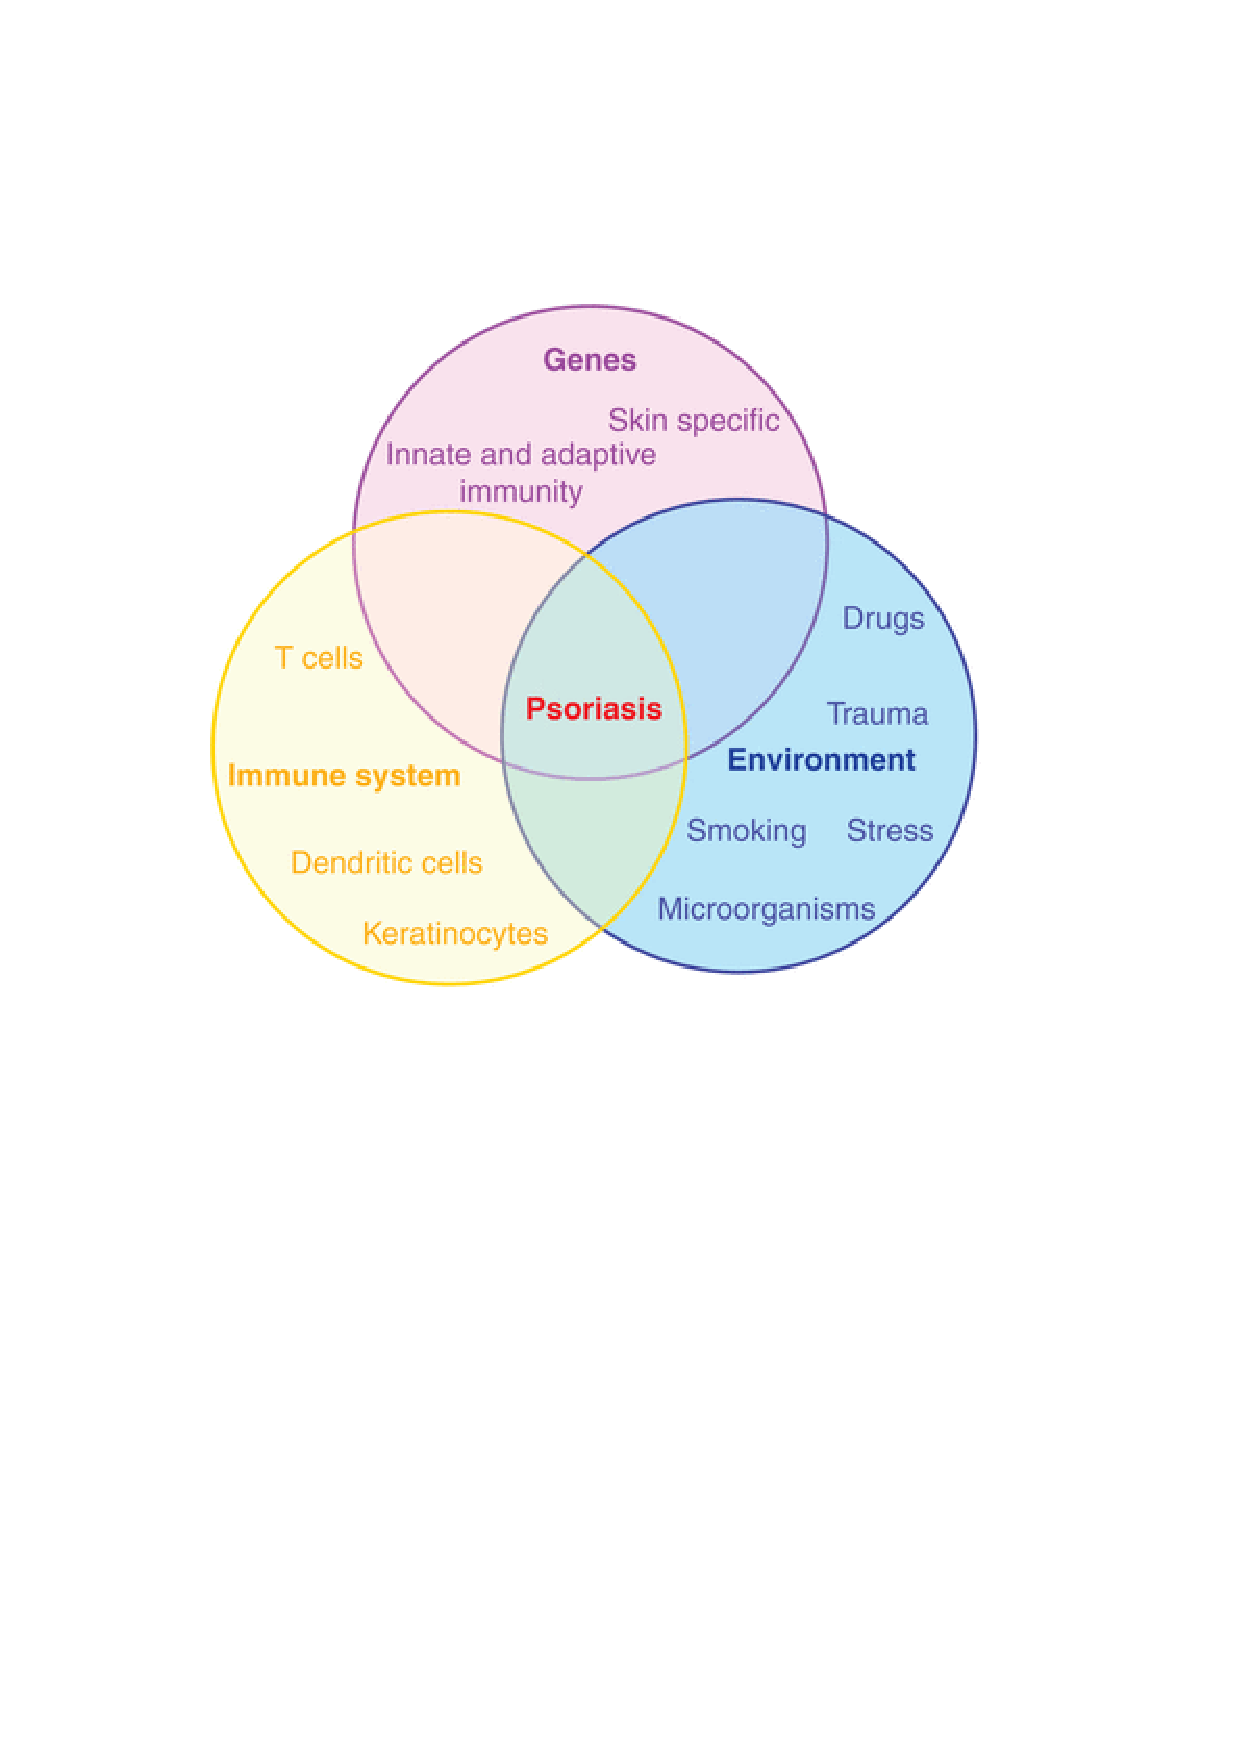
\includegraphics[width=\textwidth]{./Introduction/pdfs/PSO_aetiology_diagram_Di_Meglio_et_al_2014.pdf}
%\caption[Main factors involved in psoriasis disease aetiology]{\textbf{Figure adapted from \parencite{Meglio2014}}}
%\label{fig:PSO_aetiology_diagram}
%\end{figure}


\subsubsection{Histopathological alterations in skin and joints}

The epidermis is the most external structure of the skin and it is formed by approximately 90\% keratinocytes (KC) organised in a layer structure that self-renews in a time dependent manner from the bottom to the surface \parencite{Wikramanayake2014}. As the KC differentiate they undergo changes in morphology, replication ability and keratin composition of their intracellular matrix. In the context of psoriasis impaired epidermis cell renewal leads histological alterations and development of the psoriatic lesions. KC undergo upregulation in the proliferation rate (hyperplasia) that causes aberrant cell differentiation (parakeratosis) (ref) thickening of the epidermis and the subsequent scale formation (ref). Concomitantly, inflammation causes immune cell infiltration and hypervascularisation of the lesion driven by upregulation in the expression of angiogenic factors and activation of the endothelium \parencite{Perera2012}. 

In PsA, joint affection usually follows skin lesions and it involves a wide range of histological changes in the joints, particularly bone remodeling \parencite{Haddad2013}. One of the most common structural changes is the arthritis caused by the swelling and inflammation of the joints \parencite{Schett2011}. As result of this inflammation, alterations in bone remodeling leads to osteolysis with subsequent bone resorption and erosion at the affected joints \parencite{Mensah2017}. This phenomenon is particularly relevant in arthritis mutilans or chronic absortive arthritis, one of the most severe forms of PsA \parencite{Haddad2013}. Bone erosion is also the main histopathological process driving dactylatis, where bone lysis resolves in shortening of the digits \parencite{Gladman2005}. On the other hand, 35\% of the PsA patients undergo inflammation of the connective tissue at the insertion of tendons or ligaments, phenomenon known as enthesitis \parencite{McGonagle2011,Polachek2017}. Overtime, this causes debilitating structural changes due to formation of bony spurs along the insertion sites\parencite{Schett2011}.


\subsubsection{Dysregulation of the innate and adaptive immune response}
%link to the histological changes
The dysregulated  immune response in psoriasis and PSA is the result of the interaction between innate and adaptive immune cells (ref section) resulting in feedback loops involving a complex cytokine milieu. Among the most relevant cytokines of the innate immunity involved in disease initiation are IFN-$\alpha$ and IFN-$\gamma$ \parencite{Leanne2009}. They are mainly produced by circulating plasmacytoid DC (pDC) and myeloid DC (mDC), respectively, upon activation by KC proinflammatory cytokines \parencite{Perera2012}. Both are upregulated at the mRNA level in the lesional skin and contribute to lymphocyte recruitment and maintenance of DC activation \parencite{Schmid1994}. 

Another key cytokine in this dysregulated inflammatory response is TNF-$\alpha$ which has a prominent role in bone turnover and bone remodeling in PsA \parencite{Mensah2008}. It is produced by activated KC, mast cells but also by adaptive immune cells types, including infiltrated T helper(Th) 1 and Th17 cells infiltrated in the psoriatic lesion and PsA inflamed joints \parencite{Perera2012} and it induces activation of nuclear nactor kappa-light-chain-enhancer of activated B cells (NF-$\kapa$B) signaling pathways (ref). It also activates several kinase signaling pathways as well as cell death programs (ref). In the context of inflammation, NF-$\kapa$B represents a master transcriptional regulator of both, the innate and adaptive immune system that induces expression of proinflammatory cytokines, antiapoptotic genes and genes involved in chronic inflammation maintenance (ref). The importance of this transcription factor (TF) in psoriasis and PsA pathogenesis is reflected by the association with disease of several genetic variants in some of the negative regulators of its proinflammatory activity, including NF-$\kapa$B inhibitor alpha \textit{NFKBIA} and TNF receptor-associated factor 3 interacting protein 2 \textit{TRAF3IP2} (ref).
 
Interleukin-23 (IL23) and Th17 axis represents a key loop for the maintenance of psoriasis and PsA inflammatory response and a very important link between innate and adaptive immunity. IL-23 is an innate regulatory cytokine, mainly produced by mDC and macrophages homing the inflamed skin and it binds to the IL23 receptor (IL23R), which expression is upregulated in the DC and T cells of the lesion and in circulating Th cells (ref). In psoriasis, IL23 is the mediator for the pathogenic loop between activated KC and T cells (ref). Both IL-23 and IL-23R present protective and pathogenic genetic variants associated with psoriasis and PsA risk (ref). The activation of the IL-23 pathway leads importantly to increased IL17 production through NF-\kappaB activation by \textit{TRAF3IP2} (ref). IL17 favors maintenance of the adaptive immune mediated Th17 response through recruitment and activation of neutrophils, induction of proinflammatory cytokines including IL-1\beta and IL-6 and also perpetuation of KC activation (ref) (https://www.ncbi.nlm.nih.gov/pmc/articles/PMC3580541/). % add info
More recently, interleukin 22 (IL22) has arisen as another of the key cytokines in mediating the dysregulated cross talk between the innate and adaptive immune response. IL22 levels are increased in the psoriatic lesions and serum of patients and it is mainly produced by a subset of CD4$^+$ cells known as Th22 (ref). It mediates some of the histological changes in skin as well as AMP production by KC (ref).

% Maybe a paragraph to connect skin and joint affection Identical T cell clonality between skin and synovium https://ac.els-cdn.com/S0198885999000348/1-s2.0-S0198885999000348-main.pdf?_tid=5efa7316-fde5-11e7-8091-00000aacb360&acdnat=1516454913_dd20efb867f822d68d8b09873601e8ad

\subsubsection{Environmental factors and disease}

There are several environmental triggers known to be associated with increased risk and worsening of psoriasis and PsA development. A wide range of drugs including antidepressant, antihypertensive and anticytokine therapies have been clinically associated with initiation, exacerbation and worsening of psoriasis. As examples, therapies such as IFN-\alpha for the treatment of hepatitis C virus and anti-TNF antibodies for the treatment of several chronic inflammatory diseases, including psoriasis \parencite{Kim2010}.

Preceding streptococcal throat infection has likewise been associated with development of type I psoriasis lesions only \parencite{Gudjonsson2003}. This is partially explained by the molecular mimicry found for several streptococcal antigens, such as the M protein (highly similar to the structure of certain human keratins) and bacterial peptidoglycans \parencite{Valdimarsson2009}. Also, there is evidence of homologous T cell clones homing tonsils and psoriatic lesions \parencite{Diluvio2006}. Recent studies looking at the microbiome and disease development have also suggested perturbation in the composition of the gut and skin microbiota of psoriasis and PsA patients compared to the controls \parencite{Yan2017}. Consistently with other chronic inflammatory disease such as IBD and AS, these differences in the microbiome could lead to dysregulation of inflammatory pathways in skin and joints through immunomodulation \parencite{Eppinga2014}.

Physical trauma, including tattoos and surgical incisions, has also been associated with the appearance of psoriatic lesions in uninvolved skin as well as joint inflammation in digits \parencite {Nestle2009} due to initiation of the Koebner phenomenon \parencite{Weiss2002}. Lastly, there are several behavioral factors such as smoking, alcohol and stress with suggested with psoriasis and PsA. However, there are not consistent conclusions of their involvement in triggering disease \parencite{Meglio2014}.

\subsection{Cell types involved in psoriasis and PsA pathogenesis}
%Global report on psoriasis, 2016

There is great debate about the most relevant cell types contributing to psoriasis and PsA pathogenesis. Progressively, both are understood as dynamic and continuous processes where different cell types became predominantly important at different stages of the pathology. Regarding levels of circulating immune cells, severe psoriasis patients (PASI>12) showed significantly decreased numbers of PBMC compared to moderate (PASI<12) and healthy individuals \parencite{Langewouters2008}.
;
KC are one of the most relevant cell type at early stages of psoriasis pathogenesis. Several studies have shown the role of KC as immune sentinels through antigen presentation and production of antimicrobial peptides (AMP), cytokines and chemokines. There is evidence of complex formation between the cationic AMP cathelicidin or LL-37 and self-DNA/RNA released by the damaged KC in the psoriatic skin upon trigger by environmental factors \parencite{Lande2007}. It leads to initiation of the skin inflammation through activation of skin-resident DC \parencite{Nestle2005} and secretion of pro-inflammatory cytokines, importantly IL-1, IL-6 and TNF-$\alpha$, that reinforce activation of DC and Th lymphocytes \parencite{Feldmeyer2007, Arend2008, Nestle2009}. Moreover, expression of the MHC-II allows KC to act as APC and activate memory CD4$^+$ and CD8$^+$ T cells inducing a recall immune response \parencite{Black2007}. Studies in mouse models have shown development of psoriatic lesions in immunodeficient mice upon human xenotransplant of psoriasis skin only \parencite{Boyman2004}. The importance of KC in psoriasis development is also reinforced by the association with psoriasis risk of genes of the late cornified envelope (LCE) family \parencite{Tsoi2012}. Overall, these findings would support the hypothesis attributing the initiation of the chronic inflammatory response in psoriasis as the consequence of the epidermis dysfunction \parencyte{Proskch2008}. 

mDC and pDC have also been considered important innate immune cells in disease initiation \parencite{Mahil20016}. They are professional APC that induce T cell activation and the subsequent adaptive immune response. The relevance of antigen presentation in disease has been highlighted at the cellular \parencite{Rusell1972, Tiilikainen1980} and also at the genetic level with the psoriasis and PsA GWAS association of HLA-Cw*06:02 and ERAP1 \parencite{Strange2010}, which encodes for an aminopeptidase involved in the trimming of peptide antigens. Although pDC are circulating cells absent in healthy skin, they infiltrate into the lesional and uninvolved dermis of psoriasis lesions \parencite{Nestle2005} and get activated by the aforementionedd self-DNA and LL-37 complex through Toll-like Receptor (TLR)-9 \parencite{Lande2007}. In contrast, quiescent mDC are epidermal resident and upon secretion of IFN-$\alpha$ by pDC a 30-fold increase of mature mDC is observed in lesional skin but not in uninvolved or healthy tissue (ref). Different mDC subpopulation mediate the Th1 and Th17 response as well perpetuation of KC activation through IL-23 production (ref). Studies in immunodeficient psoriasis mice models have shown that blockage of downstream  IFN-$\alpha$ signaling or its production by pDC failed to induce T cell activation and onset of psoriasis \parencite{Nestle2005}. 

Neutrophils are also though to be closely involved in disease initiation through their ability to form neutrophil extracellular traps (NET)that contain host DNA and AMP, particularly LL-37 \parencite{Hu2016}. There is evidence of increased NET formation in peripheral blood and lesional skin of psoriasis patients and they seem to be contributing to pDC and CD4$^+$ T activation \parencite{Hu2016}. Neutrophils have also been identified in recent studies as one of the main sources of IL-17 production in the skin lesions \parencite{Lin2011} and they also release a wide range of proteases which some induce KC proliferation \parencite{Mahil2006}.

In the context of the innate immunity, the involvement of monocytes and macrophages in psoriasis and PsA has not been extensively studied. Resident macrophages in the healthy dermis undergo a 3-fold increase in lesional skin and they are involved in disease development through TNF$\alpha$ production \parencite{Perera2012, Mahil2016}. Different mice models for chronic psoriasiform skin inflammation have shown a key role of macrophage migration into the affected skin and TNF-$\alpha$ production for maintenance of the lesions \parencite{Stratis2006, Wang2006}. Some studies using psoriasis and PsA patients derived monocytes have also highlighted the systemic aspects of both pathologies. Psoriasis PBMC isolated monocytes have shown greater phagocytic and bactericidal activity compare to those from healthy individuals \parencite{Bar-Eli1979}. Later studies have also shown increased circulating intermediate monocytes (CD14$^{+}$ high CD16$^{+}$ high) and monocyte aggregation in psoriasis patients with subsequent enhanced platelet activation and angiogenesis \parencite {Golden2015}. %In PsA, synovial membranes levels of monocytes/macrophage metalloproteinases are comparable to those found in RA joints mediating bone erosion through differentiation of classical monocytes into osteoclasts \parencite{Hitchon2002}.

Historically, T lymphocytes have been considered one of the most relevant cell types in initiation and maintenance of psoriasis and PsA, and GWAS association with MHC-I also supports the role of T cells in disease. Report cases in humans have demonstrated that bone marrow transplantation can initiate or terminate psoriasis and, therefore, the role of bone marrow-derived T cells in disease pathophysiology \parencite{Eedy1990, Gardembas1990}. The percentage of circulating T cells in psoriasis has been reported to be dependent of severity. Different studies have shown reduced number of T cells in moderate-to-severe and severe psoriasis patients when compared to milder phenotypes and healthy controls. Despite this reduction, increased percentage of the memory populations CD4$^{+}$CD45RO$^{+}$ and CD8$^{+}$CD45RO$^{+}$ have been demonstrated in the same individuals\parencite{Lecewicz-Toruń2001,Langewouters2008}. There is still controversy regarding the total CD4$^+$ and CD8$^{+}$ abundance and CD4$^{+}$/CD8$^{+}$ ratios in PBMC, which may be due to the phenotype heterogeneity of psoriasis patients in the different studies \parencite{Lecewicz-Toruń2001,Cameron2003,Langewouters2008}. In PsA, no differences  abundance of circulatings T cells have been identified compared to healthy individuals \parencite{Costello1999}.

In healthy skin, CD4$^{+}$ and CD8$^{+}$ are found in the dermis and epidermis, respectively \parencite{Clark2006,Perera2012} and upon lesion development an increase in activated memory CD4$^{+}$CD45RO$^{+}$and CD8$^{+}$CD45RO$^{+}$ in the respective compartments can be detected as soon as 3 days after its appearance \parencite{Clark2006}, highlighting the importance of the memory population. \textit{In vivo} studies conducted in mice by Boyman and colleagues showed that development of psoriasis following engrafted human pre-lesional skin was dependent of local T cell proliferation and it did not required injection of additional factors \parencite{Boyle2013}. This supports the theory where recruitment of circulating T cells is restricted to the priming event and it is minimal afterward \parencite{Perera2012}. The relative importance of CD4$^{+}$versus CD8$^{+}$ in psoriasis initiation has been tested immunodeficient mice with pre-lesional skin xenografts followed with injection of purified activated T cell populations \parencite{Nickoloff1999}. These observations suggested a model where CD4$^{+}$ but not CD8$^{+}$ T cells where required for the progression of uninvolved to lesional skin in mice. Interestingly, injection of CD4$^{+}$ activated cells was followed by an increase in activated resident CD8$^{+}$ T cells expressing the acute activation marker CD69. It suggest a hypothesis where in the skin CD4$^{+}$ drive signaling for activation of resident T cells and the activated CD8$^{+}$ resident population are the main effector cells. In PsA, CD4$^{+}$ are significantly more abundant than CD8$^{+}$ cells in synovial tissues \parencite{Diani2015}. In contrast, CD8$^{+}$ expressing CD45RO are prevalent in the SF and they are also significantly increased when compared to controls \parencite{Costello1999}.

In addition to memory T cells, the contribution of regulatory T (Treg) cells have also been investigated to some extent due their role in immunosurveillance and self-tolerance in the context of autoimmune disease. Nevertheless, controversial results have been found regarding relative abundance and impaired function \parencite{Perera2012}. 

Based on the cytokine profile, psoriasis and PsA has been demonstrated to be a type 1 Th/Tc disease, where naive CD4$^{+}$ and CD8$^{+}$ cells get activated and proliferate in the presence of IL-12 and IFN-$\gamma$ \parencite{Austin1999,Perera2012}. Later studies also identified additional subsets including Th-17/Tc-17 and Th-22/Tc-22, which are mainly dependent on IL-23 and IL-6 for their activation, respectively \parencite{Mahil2016}. The importance Th17 cells and their IL-17 production has been assessed in skin, joints and blood, where increased IL-17 and also IL-23 mRNA and protein levels have been found in psoriasis and PsA patients compared to controls \parencite{Cai2012, reference for joints}. It has been shown that the predominant CD8$^{+}$ cells in the SF are  also IL-17 producers and their abundance correlates with markers of inflammation and structural changes in the joint \parencite{Menon2014}. This finding distinguishes PsA from other forms of arthritis such as RA and is in line with findings on skin that suggest a prominent role of CD8$^{+}$ IL-17 producing cells in the different stages of both pathologies. There is also evidence of the synergistic interaction between Th1 and Th17 cells which overall enhances the production of AMPs by KC \parencite{Kryczek2008}. Understanding of the importance of IL-17 has also led to the discovery of other immune cells producing this pivotal cytokine including innate immune lymphoid (ILC) cells and $\gamma$$\delta$ T cells which have also started to been investigated in the context of psoriasis and PsA pathophysiology and treatment \parencite{Meglio2014,Leijten2015}.
IL-17 producing cell have also been hypothesised to be responsible for the link between skin and joint lesions. Although the precise mechanisms for transition between psoriasis and PsA is unknown, studies using psoriasis and RA mice models have shown that skin lesions facilitate arthritis and joint inflammation % \parencite{}. 
It has been hypothesised that the presence of IL-17 producer cells in inflamed skin located nearby the enthesis of joint under physical stress could trigger the development of PsA.

\begin{figure}[H]
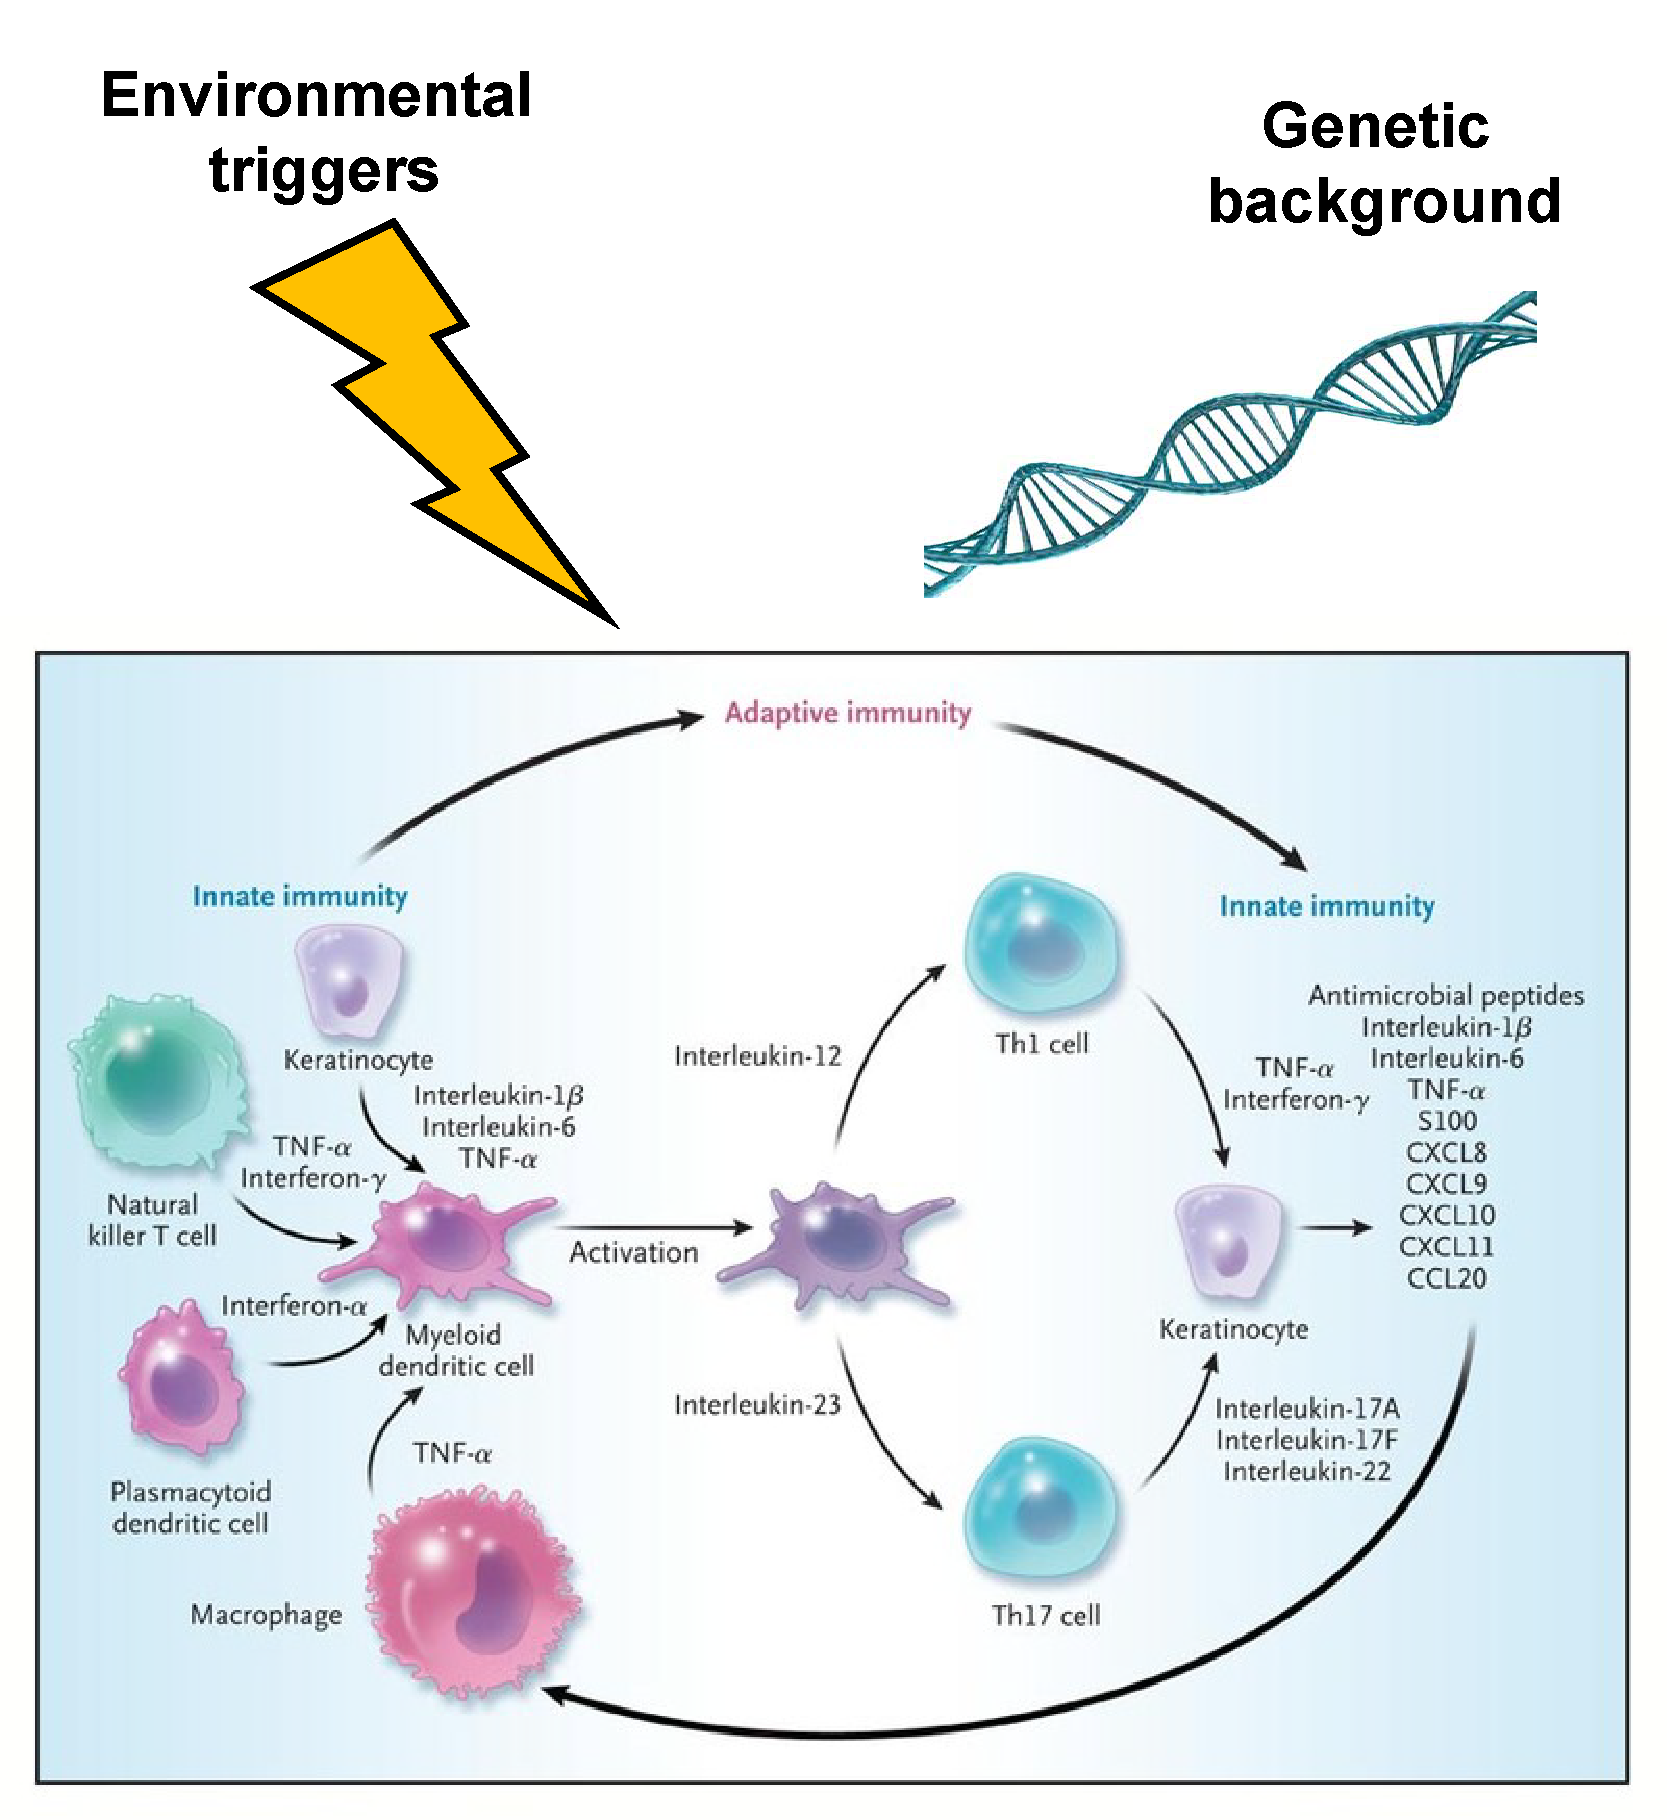
\includegraphics[width=\textwidth]{./Introduction/pdfs/PSO_adaptive_innate_immune_system_crosstalk.pdf}
\caption[Crosstalk between innate and adaptive immunity in psoriasis]{\textbf{Figure adapted from \parencite{Nestle2009}}}
\label{fig:PSO_immune_system_diagram}
\end{figure}

\subsection{Therapeutic intervention and prognosis}

Currently, there is no cure for either psoriasis or PsA and the different treatments available are focused in managing the disease manifestations and symptoms. The approach to treat them are usually dependent on the disease severity. Cases of mild-to-moderate psoriasis are usually managed with topical and systemic therapies \parencite{Menter2009}. Among the topical agents, corticosteroids and emollients are the most commonly used and affordable ones. Emollients are non-medicated agents that contribute to keep the skin soft and moist minimising the symptoms of itching and tenderness and they have been accepted as an adjunctive for the treatment of psoriasis. On the other hand, cortocosteroid in creams, shampoo and spray remain as the most widely spread medical topical treatment due to their antiinflammatory, antiproliferative, and immunosuppressive actions. Corticosteroids are classified based on the potency and they all exert their effect through binding to intracellular corticosteroid receptors and regulation of gene transcription \parencite{Tadicherla2009}. Although they are the most common way to treat mild forms of disease, some of them are approved only for short term treatments as side effects have been reported at a local and systemic level \parencite {Menter2009}. In the case of PsA presenting swelling of two or less joints intraarticular injection of glucocorticosteroids together with joint aspiration have shown to reduce pain and inflammation as a short-time measure \parencite{Coates2016}.    

For psoriasis, other topical treatments are used in combination with topical corticosteroids including ultra violet (UV) light therapy and vitamin D analogues, which inhibit KC proliferation, stimulate KC differentiation and inhibits T cell proliferation and other inflammatory mediators \parencite{Rizova2001}. Topical retinoids and calcineurin inhibitors are also used less frequently for the treatment of psoriasis and they have shown reduced systemic absorption and better suitability for long term treatments in some studies \parencite{Weinstein2003, Menter2009}.

Treatment of most forms of PsA and more moderate-to-severe psoriasis require the use of a broad range of systemic therapies. For mild cases of PsA with involvement of less than four joints and non radiological evidence of structural changes, nonsteroidal antiinflammatory drug (NSAID) are the most commonly used to help controlling the mild inflammatory symptoms and also helping to alleviate the pain and stiffness \parencite{Coates2016}. However, the use of NSAID is not recommended in patients presenting CVD comorbidities due to the increased risk associated with the use of these drugs \parencite{Bhala2013}. For those NSAID-resistant or more severe forms of PsA, disease-modifying antirheumatic drugs (DMARDs) including the an antagonist of folic acid methotrexate (MTX) and the phosphodiesterase 4 inhibitor apremilast have shown to immunosupressive effects on activated T cells and reduction of cytokine production, respectively \parencite{Schmitt2014, Gossec2016, Keating2017,Polachek2017}. However, increased risk of hepatotoxicity for the MTX \parencit{Menter2009} and gastrointestinal side effect  of apremilast \parencit{Menter2009} require requires ensuring appropriate dosing and surveillance. 


The use of biologic systemic agents tend to be the most specific but also expensive treatment for severe cases of psoriasis and PsA and they are not used as the first-line of treatment. These are molecular species generated in cell-based that modulate the immune response in a physiological based manner \parencite{Perera2012}. Among the biologic agents targeting cytokines, TNF$\alpha$ inhibitors (TNFi) have been broadly used for the past five decades to treat both, psoriasis and PsA since this is a pivotal cytokine in initiation and perpetuation of the inflammatory response. There are three TNFi approved for the treatment of psoriasis etanercept, infliximab and adalimumab \parencite{Ahil2016} and another two, certolizumab pegol and golimumab, also used in the management of PsA and other rehumatoid diseases  \parencite{Coates2016b}. All the TNFi are antibody-based agents but etanercep, that is a soluble receptor, and they also show differences in the frequency and via of administration as well as the efficacy, particularly in the specific improvement of skin or joint lesions \parencite{Mease2000}. Although TNF-$\alpha$ blockade is one of the most effective treatments some patients experience common side effects such as increased risk of infection, reactivation of latent infections, demyelinating disease and induced pustular psoriasis have been identified \parencite{Nickoloff2004}. Between 20 to 50\% of the patients fail to respond to the first TFNi and require switching to a second or third one \parencite{Abramson2016}. Lately, new biologic therapies have been developed to target other key cytokines in the pathogenesis of PsA and psoriasis, such as IL-12, IL-23 (ustekinumab) or  IL-17 (secukinumab and ixekizumab) \parencite{Mahil2016}. These new biologics represent a substantial benefit for treating patients and they are routenely administered to individuals failing to respond after a switch to a second TNFi \parencite{Coates2016b}.
 

indirect evidence mDC also produce interleukin 12 (IL12) that could contribute to IFN-$\gamma$ production in lesional skin and inflammed synovium (ref). 

%\subsection{GWAS and functional genomics of psoriasis and other complex diseases}
%\textbf{HLA-C*06:02 mediated pathogenesis}
%The association of the allele HLA-C*06:02 with PSO was first established through serological studies \parencite{Rusell1972, Tiilikainen1980} and it was later on confirmed the association of the region through genetic studies (Ellinghaus et al., 2010; Strange et al., 2010; Stuart et al., 2010; Sun et al., 2010)
%
%the  identification of the precise gene within the associated region of the genome is challenging. Although some earlier studies using microsatellites as markers excluded HLA-C, later genetic studies using dense genotyping that allows better haplotype definition have confirmed HLA-C*06:02 as the susceptibility allele and have identified a single nucleotide polymorphism (SNP) within the gene to drive the greatest association  to disease \parencite{Nair2006, Nair2009} showing 10-fold increase of PSO risk in homozygosis \parencite{Perera2012}
%
%
%number of HLA-C alleles 2375 encoding for 1677 proteins \parencite{Robinson2013}. Particularly, HLA-Cw*06 has 51 different subtypes 
%Regarding allele frequency it changes among ethnic populations. 5553 British Caucasian individuals from the OBB HLA-C allele of greater frequency was HLA-C*07:01 (High resolution HLA haplotyping by imputation for a British population bioresource Neville2017)
%
%
%
%Association of HLAC with other diseases such as Hepatitis C, PsA, primary sclerosing cholangitis and Grave´s disease \parencite{Blais2011}
%
%However, the detailed role of HLA-C*06:02 in the pathogenesis of PSO remains uncertain partly due to the homology between different MHC-In and the polymorphic nature of HLA-C. 
	%Presence of SNPs in minimal promoter and enhancer region that affects expression levels of HLA-C alleles \parencite{Clop2013, Hundhausen2012}. However HLA-Cw*0602 transcript levels do not differ significantly between normal and psoriatic showing responsiveness to proinflammatory cytokines and suggesting the association is not explained by alteration in regulation of gene expression \parencite{Hundhausen2012}. 
	%Lack of functional studies showing specific antigen or interacting proteins recognised by this allele
	%
%HLA-C is  is a heterodimer consisting of a heavy chain and a light chain and expressed in the surface of most of the cells, including antigen presenting cells (APC); however it has lower expression levels and degree of polymorphism than HLA-A and HLA-B ( Low HLA-C expression at cell surfaces correlates with increased turnover of heavy chain mRNA).
%
 %The major role of HLA-C has been assumed to be in acting as a ligand for killer immunoglobulin receptors (KIRs) expressed on natural killer (NK) cells however it is also recognised by TCR of CD8+ cells, not being clear if it exerts its pathogenic role through T cell or NK regulation 
%APC can activate immune response through presentation of processed antigens to CD8+ T cells, very abundant in the lesional epidermis due to inflitration that antigen could be T cell recognition of self-peptides hypothesis reinforced by epistasia with ERAP1 \parencite{Strange2010}, which encodes for an aminopeptidase involved in the trimming of peptide antigens. ERAP1  locus  is  only  associated  with  PSO  in  individuals carrying the HLA-C risk allele. The presentation of autoantigens(Although there are some studies regarding the self-tolerance and presence of autoantigenes as disease trigger \parencite{Lande2007}, the autoimmune aetiology of PSO is still under debate) to CD8+ T cells that clonally expand in psoriasis lesions has been reinforced by the observation of melanocytes as skin-specific target cells of an HLA-C*06:02-restricted psoriatic T cell response. We found that a CD8+ TCR, which we had reconstituted from an epidermal CD8$^+$ T cell clone of an HLA-C*06:02-positive psoriasis patient specifically recognises HLA-C*06:02-positive melanocytes. we observed numerous CD8$^+$ T cells in psoriasis lesions attacking melanocytes, the only epidermal cells expressing ADAMTSL5. Furthermore, ADAMTSL5 stimulation induced the psoriasis signature cytokine, IL-17A %reinfoce 
%, in CD8$^+$ T cells from psoriasis patients only, supporting a role as psoriatic autoantigen. % fact that CD4 are not reactive to autoantigen and that they are the first infiltrated cell type
%This unbiased analysis of a TCR obtained directly from tissue-infiltrating CD8$^+$ T cells reveals that in psoriasis HLA-C*06:02 directs an autoimmune response against melanocytes through autoantigen presentation. We propose that HLA-C*06:02 may predispose to psoriasis via this newly identified autoimmune pathway \parencite{Arakawa2015}.
%
%HLA-Cw*06:02 can be recognised by the inhibitory receptor KIR2DL1 and the activatory receptor KIR2DS1.  Some studies have shown KIR2DS1 was present in 85\% of the patients but only in 51\% of the controls
%NK cells are important regulators of immune responses \parencite{Luszczek2004}. Their function extends beyond killing of infected or transformed cells. Interactions with dendritic cells, macrophages, and fetal trophoblast cells can regulate NK cell activity by influencing cytokine production, cytotoxicity and stimulation of T helper-1 responses. 
%
%
%A similar inflammatory skin phenotype, which was also shown to be T-cell-dependent (Breban et al., 1996), was seen in rats transgenically expressing high levels of HLA-B27 and human β2-microglobulin (Tg(HLA-B*2705, B2M)33-3Trg; Table S1). However, these animals also developed multisystem inflammatory disease characterized by arthritis and colitis (Hammer et al., 1990).
%
%
%
 %
%
   %
%
%
%
%
%Nevertheless, other studies have demonstrated development of PSO in wild type mice upon bone marrow transplantation from mice with PSO-like phenotype
%
%
%
%
%
%
%\subsubsection*{Epigenetics and gene expression}
%\textbf{Understanding the chromatin landscape}
%\textbf{Chromatin accessibility}
%\textbf{Histones modifications}
%\textbf{Understanding the chromatin landscape}
%\textbf{Transcription factor occupancy}
%\textbf{Chromatin interaction}
%
%
%% For later when talking about cohort Approximately one third of patients have moderate to severe disease, which affects more than 10 % of body surface area, and usually necessitates systemic medications.	
\chapter{Material and Methods}
\label{ch:Mat}


%%%%%%%%%%%%%%%%%%%%%%%%%%%%%%%%%%%%%%%%%%%%%%%%%%

\section{Ethical approval and recruitment of study participants}
Sample recruitment for the two different phenotypes and the healthy volunteers were conducted under different ethics.

\subsection{Psoriasis patient recruitment}

Patient blood samples and normal or psoriatic skin biopsies were collected in collaboration with the Dermatology Department research nurses at the Churchill Hospital, Oxford University Hospitals NHS Trust and Professor Graham Ogg at the Weatherall Institute of Molecular Medicine, University of Oxford under approval from the Oxfordshire Research Ethics Committee (REC 09/H0606/71 and 08/H0604/129). After written informed consent, up to 60 mL of blood from eligible psoriasis patients were collected into 10 mL anticoagulant EDTA-containing blood tubes (Vacutainer System, Becton Dickson).

Psoriasis patients were eligible for recruitment when meeting the following criteria:
\begin{itemize}
  \item over 18 years old
  \item previously or newly diagnose, in a flare and going into biologic therapy for the first time % check with Graham
	\item fulfillment of the clinically accepted Psoriasis Area and Severity Index (PASI) classification for psoriasis diagnosis \parencite{Fredriksson1978}
	\item moderate to severe disease (PASI>5) % check with Graham
	\item less than 2 weeks without antibiotics unless used for prophylaxis % check with Graham or research nurses
	\item available clinical information and written consent
\end{itemize}

Detailed clinical information of the psoriasis cohort is included in %(Chapter \ref{ch:})(Table \ref{tab:}).

\subsection{PsA patient recruitment}
Sample recruitment was performed as part of the Immune Function in Inflammatory Arthritis (IFIA) study established in 2013 (REC/06/Q1606/139)in collaboration with research nurses at the Nuffield Orthopaedic Centre, Oxford University Hospitals NHS Trust and Dr Hussein Al-Mossawi at the Botnar Research Centre. Following informed written consent, blood (30 mL) and synovial fluid aspirate (variable upon disease severity) were recruited into 10 mL anticoagulant sodium heparin coated tubes (Vacutainer System, Becton Dickson).

Eligibility of the PsA patients was upon fulfillment of the following criteria:
\begin{itemize}
  \item over 18 years old
  \item previously or newly diagnose, with concomitant psoriasis, in a flare and going into biologic therapy for the first time % check with Hussein
	\item fulfillment of the clinically accepted PsA Response Criteria (PSARC) including a physician global assessment questionnaire \parencite{Philipp2011,Clegg1996}
	\item oligoarticular phenotype and na\"{i}ve for any treatment
	\item less than 2 weeks without antibiotics unless used for prophylaxis % check with Hussein
	\item available clinical information and written consent
\end{itemize}

Further details about the cohort and clinical information can be found in (Chapter \ref{ch:})(Table \ref{tab:}).

\subsection{Healthy volunteer recruitment}
Recruitment of healthy volunteers was conducted as part of the study Genetic Diversity and Gene Expression in White Blood Cells with approval from the Oxford Research Ethics Committee (REC 06/Q1605/55). Up to 80 mL of blood were collected into 10 mL anticoagulant EDTA-containing blood tubes, similarly to the psoriasis sample recruitment.

The criteria for healthy individuals to participate in the study was:
\begin{itemize}
  \item over 18 years old and preferably British or European
  \item no family history of psoriasis, PsA, RA or SpA
	\item matched sex and age with the psoriasis cohort
	\item less than 2 weeks since last infectious process
	\item available clinical information and written consent
\end{itemize}


\section{Sample processing}
\label{sample_processing}
Blood, synovial fluid and skin biopsies were processed straight after recruitment following the appropriate protocols.

\subsection{PBMC and synovial fluid cells isolation}
PBMC were isolated from blood samples through density gradient separation using Ficoll-Paque. Total synovial fluid (SF) cells (SFC) were isolated by centrifugation at 500g for 5 min. Both were washed twice in Hank’s balanced salt solution without calcium or magnesium (Thermo Fisher Scientific) and resuspended in phosphate saline buffer (PBS, Gibco) supplemented with 0.5\% fetal calf serum (FCS, Invitrogen) and 2mM ethylenediaminetetraacetic acid (EDTA, Sigma)prior to cell types separation. Cell numbers and viability were determined by manual count using a haemocytometer and trypan blue (Sigma).

\subsection{Primary cell isolation using magnetic-activated cell sorting}
For the work related to psoriasis and healthy volunteers, primary cell subpopulations were separated using magnetic-activated cell sorting (MACS, Miltenyi). Positive selection was performed for consecutive isolation of CD19$^{+}$ B cells, CD8$^{+}$ T cells, CD14$^{+}$  monocytes and CD4$^{+}$ T cells with AutoMACS Pro (Miltenyi) and cells were manually counted as previously described. MACS separation was chosen over Fluorescence-associated cell sorting (FACS) due to time and logistic constrains in the sample processing and therefore cell numbers in down stream application may not be as exact.

\subsection{Primary cell isolation using fluorescence-activated cell sorting}
Primary cell subpopulations from controls to study the effect of cryopreservation in chromatin states (Chapter 3) or PsA blood and SF samples were isolated by FACS. PBMC and SFC were resuspended in PBS 1mM EDTA (FACS buffer) at 10x10$^6$ cells/mL, stained with the appropriate antibody cocktail (Table \ref{tab:FACS_antibodies}) for 30 min at 4{$^\circ$}C, washed with FACS buffer and centrifuged at 500g for 5 min at 4{$^\circ$}C. For the samples used in Chapter 3, a modified FACS buffer supplemented with 3 mM EDTA , 2\% FCS and 25mM 4-(2-hydroxyethyl)-1-piperazineethanesulfonic acid (HEPES, Invitrogen) was used to avoid cell clumping after cryopreservation and short recovery.After removing the supernatant, cells were resuspended in FACS buffer prior to separation. 

In the controls samples of Chapter 3 only CD14$^{+}$ monocytes and CD3$^+$ CD14$^{-}$ CD4$^{+}$ T cells were isolated in the SONY SH800 cell sorter. For the PsA samples, separation of  CD19$^{+}$ B cells, memory T cells (CD3$^{+}$ CD14$^{-}$ CD4$^{+}$ CD45RA$^{-}$ and CD3$^{+}$ CD14$^{-}$ CD8$^{+}$ CD45RA$^{-}$) ,CD14$^{-}$ monocytes and CD56$^{-}$ NK was performed using FACS Aria (BD) cell sorter from both PBMC and SFC. Bulk sorted cells were collected in 1.5mL tubes in PBS 1\% FCS, whilst single cell and small bulk sorting was performed in 96-well plates in the appropriate buffer (See RNA-seq section). Different nozzle sizes were chosen for bulk and single-cell sorting and OneComp eBeads (eBioscience) were used for compensation of fluorescence spill over.


\begin{table}[htbp]
%\setlength{\tabcolsep}{20pt} only to stretch the columns if you want
%\renewcommand{\arraystretch}{1.5}
\begin{tabular}{@{} c c c c c}
\toprule
\textbf{Surface} & \textbf{Fluorochrome} & \textbf{Manufacturer} & \textbf{Clone} & \textbf{Dilution} \\
\textbf{marker} & \textbf{PsA/CTL} & \textbf{PsA/CTL} & \textbf{PsA/CTL} & \textbf{PsA/CTL} \\
\midrule
\midrule
Viability & eFluor780 & - & eBioscience & 1:250\\
CD3 & FITC/AF700 & SK7/UCHT1 & BioLegend & xxx/1:50\\
CD4 & APC & RPA-T4/RPA-T4 & BioLegend & 1:50/1:50\\
CD8a & PE & RPA-T8 & BioLegend & xxx\\
CD45RA & BV421 & HI100 & BioLegend & xxx\\
CD19 & PerCP-Cy5.5 & SJ25C1 & BioLegend & xxx\\
CD14 & Pe-Cy7/FITC & M5E2/TUK4 & BioLegend/Miltenyi & xxx/1:100\\
CD56 & BV510 & NCAM16.2 & BD & xxx\\
\bottomrule
\end{tabular}
\medskip %gap
\caption[Antibody panel used for FACS separation of primary cell populations in controls and PsA samples]{\textbf{Details regarding target molecule, fluorochrome, clone, supplier and dilution used for PBMC and SFC staining are provided for each of the antibodies in the panel. In controls only CD3, CD4 and CD4 markers were used.}}
\label{tab:FACS_antibodies}
\end{table}
\bigskip %bigger space



%Long table example
%\begin{longtable}{ p{.15\textwidth} p{.25\textwidth} p{.2\textwidth} p{.15\textwidth} p{.15\textwidth}}
%\caption[Antibody panel used for FACS separation of primary cell populations in controls and PsA samples]{\textbf{Details regarding target molecule, fluorochrome, clone, supplier and dilution used for PBMC and SFC staining are provided for each of the antibodies in the panel. In controls only CD3, CD4 and CD4 markers were used.}}
%\label{tab:FACS_antibodies} \\
%
%\toprule
%\textbf{Surface marker} & \textbf{Fluorochrome PsA/controls} & \textbf{Manufacturer PsA/controls} & \textbf{Clone PsA/controls} & \textbf{Dilution PsA/controls} \\
%\midrule
%\midrule
%Viability & eFluor780 & - & eBioscience & 1:250\\
%CD3 & FITC//AF700 & SK7/UCHT1 & BioLegend & xxx/1:50\\
%CD4 & APC & RPA-T4(RPA-T4) & BioLegend & 1:50/1:50\\
%CD8a & PE & RPA-T8 & BioLegend & xxx\\
%CD45RA & BV421 & HI100 & BioLegend & xxx\\
%CD19 & PerCP-Cy5.5 & SJ25C1 & BioLegend & xxx\\
%CD14 & Pe-Cy7/FITC & M5E2/TUK4 & BioLegend/ Miltenyi & xxx/1:100\\
%CD56 & BV510 & NCAM16.2 & BD & xxx\\
%\bottomrule
%\medskip %gap
%
%\end{longtable}
%\bigskip %bigger space
%









\subsection{Skin biopsies processing and adherent assay}
KC enrichment from skin biopsies was performed as described in Gutowska-Owsiak and colleagues \parencite{Gutowska‐Owsiak2012}. Skin biopsies (approximately 4mm) were washed with PBS, cut in 1mm width strips and incubated in 2U/mL of dispase II (Sigma) overnight at 4{$^\circ$}C. The epidermis was separated from the dermis and either snap-frozen in liquid nitrogen (for RNA extraction) or further digested in trypsin (Invitrogen) at 37{$^\circ$}C for 5 min, when used for chromatin accessibility assay. After digestion the resulting cell suspension was filtered through a 70$\micro$m nylon strainer (BD) and washed with PBS. In some instances cells were manually counted and aliquoted for ATAC-seq processing. In others, cell from each of the biopsies were resuspended in KGM-2 BulletKit (Lonza) supplemented with 0.06mM Ca$^2{+}$ and cultured in a collagen IV coated 96-well plate at 4{$^\circ$}C for 10 min or 3 hours, upon experimental requirements (see Chapter X). After culturing, cells were washed twice with 200$\micro$L of PBS and kept at 37{$^\circ$}C for downstream processing.



\section{Experimental protocols}
\subsection{Cryopreservation and cell culture}
For the controls samples in Chapter 3, 40-50x10$^6$ of PBMC were freeze-thawing using a modified version of the \parencite{Kent2009} protocol, where cells were pre-conditioned in RPMI 1640 (brand) complete medium supplemented with2 mM L-glutamine, 100U penicillin and strep 100$\micro$g/mL and 50\% FCS for 30 minutes and afterwards diluted 1 in 2 in complete RPMI 1640 (supplemented as previously described) with 20\% dimethyl sulfoxide (DMSO, Sigma). PBMC underwent slow cryopreservation at -80{$^\circ$}CC in isopropanol at -1{$^\circ$}C per minute and stored for a minimum of two weeks in liquid nitrogen. PBMC were thaw, resuspended in supplemented complete RPMI 1640 with 10\% FCS at a density of 10$^6$ cells/mL and rested for 30 min at 37°C, 5\% CO2 in 25mL non-adherent polypropylene cell culture flasks followed by filtering through a 40$\micro$m to obtain an homogenous cell suspension undergoing FACS separation.
%
Frozen Normal human epidermal keratinocytes (NHEK) in passage 3 were recovered and cultured at a cell density of 5x10$^6$ cells/mL in a 75 mL adherent cell culture flask (brand) in EpiLife basal medium (Gibco) following manufacturer's instructions. After recovery NHEK were trypsinised at room temperature for 8 minutes followed by trypsin inactivation with EpiLife 10\% FCS, centrifugation at 180g for 10 min at room temperature and manual counting with trypan blue. NHEK were seeded in a 96-well plate in 100uL of medium at a cell density of 160 cells/$\micro$L. NHEK were cultured for 2 days to a 90-100\% confluence before being used downstream.

\subsection{ATAC-seq, Fast-ATAC and Omni-ATAC}
Improved versions of the ATAC-seq protocol were progressively used in the thesis for assessment of chromatin accessibility in different primary cells, including CD14$^{+}$ monocytes, CD4$^+$ and CD8$^+$ T cells, CD19$^+$ B cells and CD56$^+$ NK cells. The subsequent version aimed to reduce the amount of mitochondrial DNA and improve the ratio of signal to noise for this technique.

After MACS separation, primary cells were manually counted as above specified and they were resuspended in PBS with 1\% FCS. As previously stated, due to reduced accuracy of manual cell counting compared to FACS sorting, in my experiments ATAC-seq was performed using an estimated number of cells between 50,000 to 100,000. ATAC-seq was performed as described in Buenrostro \textit{et al.}, 2013 with minor modifications. Cells were centrifuged at 500g for 5 min at 4{$^\circ$}C. After removing the supernatant cells were lysed for 10 min, the nuclei were transposed using the Nextera Tn5 transposase (Illumina) for 40 min at 37{$^\circ$}C and DNA was purified using the PCR MinElute kit (Qigen). Additional modifications and performance in 96-well plates were implemented for KC and they will be described in %(Chapter \ref{ch:}). 

After appropriate determination of the amount of DNA amplification using qPCR, samples were amplified and singled indexed for 11 PCR cycles using modified Nextera primers from Buenrostro \textit{et al.},2013 (Table\ref{tab:Indexing_primers}). The resulting DNA libraries were purified using the MinElute PCR purification kit  (Qiagen) and additional Agencourt AMPure XP Magentic Beads (Beckman Coulter), according to the manual specifications, to remove the remaining adaptors and primer dimers.

\begin{landscape}
\begin{table}[htbp]
\setlength{\tabcolsep}{20pt}
%\renewcommand{\arraystretch}{1.5} makes it longer
\begin{center}
\begin{tabular}{@{} c c}
\toprule
\textbf{Primer name} & \textbf{Full sequence} \\
\midrule
\midrule
Ad1.noMX & AATGATACGGCGACCACCGAGATCTACACTCGTCGGCAGCGTCAGATGTG \\
Ad2.1 & CAAGCAGAAGACGGCATACGAGAT\textcolor{blue}{TCGCCTTA}GTCTCGTGGGCTCGGAGATGT \\
Ad2.2 & CAAGCAGAAGACGGCATACGAGAT\textcolor{blue}{CTAGTACG}GTCTCGTGGGCTCGGAGATGT \\
Ad2.3 & CAAGCAGAAGACGGCATACGAGAT\textcolor{blue}{TTCTGCCT}GTCTCGTGGGCTCGGAGATGT \\
Ad2.4 & CAAGCAGAAGACGGCATACGAGAT\textcolor{blue}{GCTCAGGA}GTCTCGTGGGCTCGGAGATGT \\
Ad2.5 & CAAGCAGAAGACGGCATACGAGAT\textcolor{blue}{AGGAGTCC}GTCTCGTGGGCTCGGAGATGT \\
Ad2.6 & CAAGCAGAAGACGGCATACGAGAT\textcolor{blue}{CATGCCTA}GTCTCGTGGGCTCGGAGATGT \\
Ad2.7 & CAAGCAGAAGACGGCATACGAGAT\textcolor{blue}{GTAGAGAG}GTCTCGTGGGCTCGGAGATGT \\
Ad2.8 & CAAGCAGAAGACGGCATACGAGAT\textcolor{blue}{CCTCTCTG}GTCTCGTGGGCTCGGAGATGT\\ 
Ad2.9 & CAAGCAGAAGACGGCATACGAGAT\textcolor{blue}{AGCGTAGC}GTCTCGTGGGCTCGGAGATGT \\
Ad2.10 & CAAGCAGAAGACGGCATACGAGAT\textcolor{blue}{CAGCCTCG}GTCTCGTGGGCTCGGAGATGT \\
Ad2.11 & CAAGCAGAAGACGGCATACGAGAT\textcolor{blue}{TGCCTCTT}GTCTCGTGGGCTCGGAGATGT \\
Ad2.12 & CAAGCAGAAGACGGCATACGAGAT\textcolor{blue}{TCCTCTAC}GTCTCGTGGGCTCGGAGATGT \\
Ad2.13 & CAAGCAGAAGACGGCATACGAGAT\textcolor{blue}{ATCACGAC}GTCTCGTGGGCTCGGAGATGT \\
Ad2.14 & CAAGCAGAAGACGGCATACGAGAT\textcolor{blue}{ACAGTGGT}GTCTCGTGGGCTCGGAGATGT \\ 
Ad2.15 & CAAGCAGAAGACGGCATACGAGAT\textcolor{blue}{CAGATCCA}GTCTCGTGGGCTCGGAGATGT \\
Ad2.16 & CAAGCAGAAGACGGCATACGAGAT\textcolor{blue}{ACAAACGG}GTCTCGTGGGCTCGGAGATGT \\
Ad2.22 & CAAGCAGAAGACGGCATACGAGAT\textcolor{blue}{TGTGACCA}GTCTCGTGGGCTCGGAGATGT \\
Ad2.23 & CAAGCAGAAGACGGCATACGAGAT\textcolor{blue}{AGGGTCAA}GTCTCGTGGGCTCGGAGATGT \\
\bottomrule
\end{tabular}
\medskip %gap
\caption[Modified Illumina Nextera indexing primers]{\textbf{Name and full sequence of the PCR primers used for amplification, indexing and pooling of the ATAC-seq and ChIPm samples in this thesis. These primers were designed by Buenrostro \textit{et al.}, 2013 and they are an modified version of the Nextera Illumina primers optimised for larger molecular weight DNA fragments from low input samples. All samples were indexed with the universal primer Ad1.noMx and one of the additional 18 primers. The indexing sequence of each of the primers is in blue text.}}
\label{tab:Indexing_primers}
\end{center}
\end{table}
\end{landscape}
\bigskip %bigger space

Following the Nature Methods publication of Corces et al., 2016, the  initial ATAC-seq protocol was replaced by a modified version named Fast-ATAC. It was specifically optimised for hematopoietic cells and combined cell lysis and transposition in a single step. Fast-ATAC was performed as described by Corces et al., 2016 with minor modifications. Since 5,000 cells was considered the lower limit to generate good quality data in Fast-ATAC, in my experiments I used 20,000 MACS or FACS sorted cells, to account for inaccurate manual cell counting as well as possible cell loss over centrifugation steps. The Fast-ATAC reaction was performed for 30 min at 37{$^\circ$}C and agitation at 400rpm. DNA was purified as in ATAC-seq and libraries were generated following 13 cycles of PCR amplification, following appropriate cell cycle determination. Purification following PCR were performed using Agencourt AMPure XP Magentic Beads only.

Omni-ATAC, a third generation of ATAC-seq was published by Corces et al., 2017. It consisted in an universal protocol with individual cell lysis and transposition reactions intercalated with a washing step, to remove mitochondrial DNA and other cell debri %check. 
Omni-ATAC was performed as described by Corces and colleagues \parencite{Corces2017} using 50,000 cells.

Following either of the three protocols, DNA tagmentation profiles were assessed with the D1000 high sensitivity DNA tape (Agilent) as part of the quality control and quantified using the Kapa kit (Roche), following the manufacturer's instructions. Pools of 12 to 16 libraries were sequenced in one to 3 lanes of the HiSeq4000 Illumina platform by the Oxford Genomics Centre at the Wellcome Trust Centre for Human Genetics to achieve approximately 50 million paired-end reads.


\subsection{Chromatin Immunoprecipitation with sequencing library preparation by Tn5 transposase}
Assessment of histone marks modification in the chromatin of psoriasis patients from Cohort 1B and four age matched healthy volunteers was performed using a low cell input Chromatin Immunoprecipitation (ChIP) method know as ChIPmentation (ChIPm). For each individual and cell type three histone marks, including H3K27ac, H3K4me1 and X were tested in chromatin isolated from 100,000 cells and compared to an input chromatin sample processed in parallel. Samples were processed following the protocol published by Schmidl and colleagues \parencite{Schmidl2015} with some modifications. Aliquots of 600,000 cells of MACS sorted cell types, as described in \ref{sample_processing}, were fixed with 1\% formaldehyde (Sigma) and snap frozen in dry ice and ethanol prior to storage at -80{$^\circ$}C. Chromatin sonications of the different individuals and cell types were performed in one batch using Covaris M220(Covaris). Each of the aliquots was resuspended in 130$\micro$L of SDS lysis buffer (Table\ref{tab:ChIPm_buffers}), sonicated for 8 min using a duty factor of 5\% and aliquoted for single ChIPm reactions prior to long term storage at -80{$^\circ$}C.

Sonicated chromatin aliquots were thawed and 1.5 volumes of ChIP equilibration buffer (Table\ref{tab:ChIPm_buffers}) was added in order to  reduce the SDS concentration to 0.1\% and to achieve the appropriate concentration of NaCl and Triton-X100. For the immunoprecipitation step, samples were incubated with the appropriate amount of antibody (Table \ref{tab:ChIPm_antibodies}) overnight in rotation  at 4{$^\circ$}C . Protein-A Dynabeads (Invitrogen) were also washed in beads wash buffer (Table\ref{tab:ChIPm_buffers}), blocked with yeast tRNA (Ambion) and BSA (NEB) overnight in rotation at 4{$^\circ$}C and added to the sample-antibody mix for incubation. After appropriate washes, tagmentation was performed on the bead-antibody bound crosslinked complexes, which prevents overtagmentation of the DNA. This was followed by protein K digest, reverse crosslinking, elution of the DNA and from the beads and purification using PCR MinElute kit. The chromatin input control samples were quantified with Qbit after reverse crosslinking and 1ng of chromatin was used for tagmentation.

Amplification by qPCR was done in each of the samples and control inputs to identify the number of full cycles required to reach one-third of the final fluorescence. Libraries were amplified for the number of cycles minus one determined with this strategy to minimise the total number of PCR replicates. The primers used for amplification and indexing were the ones optimised by Buenrostro and colleagues (Table\ref{tab:Indexing_primers}). The number of amplification cycles for each of the samples is recorded in %\ref{Table:}.

\begin{table}[htbp]
\begin{tabular}{@{} c c}
\toprule
\textbf{Reagent} & \textbf{Final concentration}\\
 & & \\
\bottomrule
 & \textbf{SDS lysis buffer} & \\
\midrule
\midrule
SDS & 0.25\% & Sigma \\	
EDTA	& 1mM & X \\
Tris-HCl pH 8 & 10mM & Sigma \\
PI & 1X & Roche \\
Water & - \\
\bottomrule
 & \textbf{ChIP equilibration buffer}  & \\
\midrule
\midrule
Triton-X100 & 1.66\% \\
EDTA	& 1mM \\
NaCl	& 233mM \\
Tris-HCl pH 8 & 10mM \\
PI & 1X \\
Water & - \\
\bottomrule
 & \textbf{Beads washing buffer} & \\
\midrule
\midrule
SDS & 0.1\% \\
EDTA	& 50mM \\
NaCl & 150mM \\
NP-40 & 1\% \\
Tris-HCl pH 8 & 10mM \\
PI & 1X \\
Water & - \\
\bottomrule

 & \textbf{ChIP buffer} & \\
\midrule
\midrule
SDS & 0.1\% \\
Triton-X100 & 1\% \\
EDTA	& 1mM \\
NaCl & 140mM \\
Tris-HCl pH 8 & 10mM \\
PI & 1X \\
Water & - \\
\bottomrule
\end{tabular}
\medskip %gap
\caption[ChIPm buffers modified from Schmidl \textit{et. al}, 2015]{\textbf{Composition of the three modified buffers in house for the ChIPm protocol: SDS lysis buffer, ChIP equilibration buffer, beads washing buffer and ChIP buffer. For each of the buffers the reagents, composition and supplier are indicated.The final volume prepared for each buffer was adjusted depending on the number of samples processed at the time. Sodium dodecyl sulfate (SDS), PI (proteinase inhibitor). Supplier for each of the reagents as follows: SDS (Sigma), EDTA(xxx), Tris-HCl pH8 (xx), Triton-X100 (xxx), NP-40 (Sigma) NaCl(xx), PI (Roche) and water (Ambion) }}
\label{tab:ChIPm_buffers}
\end{table}
\bigskip %bigger space

\begin{table}[htbp]
\setlength{\tabcolsep}{20pt}
\renewcommand{\arraystretch}{1.5}
\begin{tabular}{@{} c c c c}
\toprule
\textbf{Histone mark} & \textbf{Feature} &\textbf{$\micro$g per sample} & \textbf{Manufacturer}\\
\midrule
H3K27ac & Active enhancer, promoter & 2 & Diagenode (C15410196)\\
H3K4me1 & Enhancer & 1 & Diagenode (C15410194)\\
H3K4me3 & Active promoter, enhancer & 1 & Diagenode (C15410003) \\
\bottomrule
\end{tabular}
\medskip %gap
\caption[Antibody panel used for immunoprecipitation of histone marks in ChIPm]{\textbf{Details regarding the histone marks, the the most likely chromatin state delineated, the amount of antibody required per reaction and the supplier and catalog num of the antibodies.}}
\label{tab:ChIPm_antibodies}
\end{table}
\bigskip %bigger space


\subsection{RNA extraction and RNA-seq}

\subsubsection{Bulk RNA-seq}
Following MACS isolation of the different cell types from the psoriasis and matched healthy controls, between 2-3x10^6 cells were resuspended in 350$\micro$L of RNAProtect (Qiagen) or RLT buffer (Qiagen) supplemented with 0.1\% of beta-mercaptoethanol (BM, Sigma) and snap frozen in dry ice before storage at -80{$^\circ$}C. Cells isolated from psoriasis and control Cohort 1A (Chapter \ref{ch:}) were preserved in RNAProtect, which stops any biochemical reaction and transcriptional activity maintaining cell integrity. At early stages of the project, when I was uncertain of time frames to process the different material from the acquires samples, I decided to use RNAProtect to preserve cells for future RNA extraction to guarantee high quality in case storage exceeded 6 months. In the psoriasis and control samples from Cohort 1B %(Chapter \ref{ch:}) 
, cells were resuspended in 0.1\% BM supplemented RLT buffer, which lysates cells and prevents RNA degradation. Cell lysates were homogonised using the QIAshredder (Qiagen) prior to RNA extraction. When starting from RNAProtect preserved material, cells were centrifuged at 300g for 10 min at room temperature, the supernatant were removed and the pellets were resuspended in 350$\micro$L of RLT 0.1\% BM buffer, prior to homogenisation with QIAshredder.

Total RNA were extracted using the AllPrep DNA/mRNA/microRNA Universal kit (Qiagen) following the manufacturer's instructions. RNA extractions were performed in batches of 12 samples, including all cell types from each individual and a balanced numbers of psoriasis and control samples, to minimise batch effect correlation with phenotype groups. Basic quantification was performed with NanoDrop (Thermo Scientific) before storage at -80{$^\circ$}C.

RNA-seq quality control (QC), quantification, library preparation and sequencing were carried out by Oxford Genomics Centre at the Wellcome Trust Centre for Human Genetics in two independent batches of samples, each including Cohort 1A or Cohort 1B, respectively. Processing of samples in two batches was due to logistics of patients recruitment in the project. Quality control and quantification were assessed with the Bioanalyzer (Agilent). Preparation of RNA-seq libraries was performed using Ribo-Zero rRNA Removal kit (Illumina), based on ribosomal RNA depletion. Unlike strategies using polyadenylated transcripts selection, this method allowed to preserve non-polyadenylated transcripts including nascent pre-mRNA (unspliced) and functionally relevant lncRNAs. For each of the cohorts, all libraries were pooled together and  sequenced over several lanes of HiSeq4000 to a depth of 50 million total reads per sample in order to maintain an appropriate level of sensitivity for subsequent expression analysis given the greater complexity of these libraries.

 

\subsubsection{PsA memory CD4$^{+}$ and CD8$^{+}$ single-cell RNA-seq} 
\label{scRNA_processing}

Single CD4$^{+}$ or CD8$^{+}$ memory T cells were sorted in 2$\micro$L of cell lysis buffer into 96-well plates. Four and three plates were prepared for CD4$^{+}$ and CD8$^{+}$, respectively, including wells containing 50 cells in each of the plates for control purposes. Libraries were prepared,indexed and sequenced at the Sanger Institute (Cambridge) using the Smart-seq2 methodology as described by Picelli and colleagues \parencite{Picelli2014}. Samples were sequenced using 50-bp single-end Illumina HiSeq2500 at a depth of approximately 4 million reads per cell. %look in notebook for details about scRNA in Cambridge

scRNA-seq was also generated in FACS sorted 1:1 ratio CD4$^{+}$ or CD8$^{+}$ memory T cells and in bulk PBMC using 10X Genomics technology Chromium single cell 3' and 5' expression library prep kits (PN-120267 and PN-1000014, respectively) by the Oxford Genomics Centre at the Wellcome Trust Centre for Human Genetics. Libraries were sequenced with Illumina HiSeq4000 xxxbp single-end at a depth of 50,000 reads per cell.

\subsubsection{Small-bulk RNA-seq } 
Between 100 to 500 cells of the five populations isolated from PsA patients were FACS sorted into 2$\micro$L of cell lysis buffer and processed for library prep as in Picelli \textit{et al.}, 2014 by the Oxford Genomics Centre at the Wellcome Trust Centre for Human Genetics. Libraries were sequenced with Illumina HiSeq4000 xxxx bp single-end at a depth of XXX reads per cell.


\subsection{Single-cell analysis of the V(D)J T cell receptor repertoire}
Single-cell sequencing of the V(D)J segments from TCR transcripts was performed simultaneously with the 10X Genomics technology Chromium 5' expression library kit (PN-1000014) by the Oxford Genomics Centre at the Wellcome Trust Centre for Human Genetics. In short, full-length cDNA was amplified by PCR with primers against the 5’ and 3’ ends of the barcode sequences inherent to the 10X Genomics bead technology. The amplified material was divided for use in 5' total scRNA-seq (as specified previously in \ref{scRNA_processing}) and also for enrichment of the TCR by PCR amplification with specific primers. TCR enriched cDNA was followed by enzymatic fragmentation and size selection in order to obtain variable length fragments spanning the V(D)J segments. Library prep and indexing was followed by Illumina HiSeq4000 xxxx bp single-end sequencing at a depth of XXX reads per cell.

\subsection{DNA extraction and SNP genotyping}
DNA isolation was performed using the AllPrep DNA/mRNA/microRNA Universal kit (Qiagen) following the manufacturer's instructions. Basic quantification was performed using NanoDrop (Thermo Scientific) and kept at -80{$^\circ$}C for long term storage. For each of the patients and controls, the extracted DNA was amplify by PCR using forward (5'-CACTGTGGAGGGAGGAACAA-3') and reverse (5'-CGTGTTGGCCAGGATAGTCT-3')primers annealing up and down stream the SNP rs4672505, respectively. The 390 bp PCR product was purified using MinElute PCR purification kit, quantified by dsDNA Qbit kit (Invitrogen) according to the manufacturer's instructions and prepared for Sanger sequencing using the Mix2Seq service (Eurofins). The forward and reverse sequences were analysed with BioEdit software.



\subsection{Mass cytometry analysis}

Mass cytometry analysis was performed by Dr Nicole Yager in collaboration with UCB following their in-house protocol. Briefly, PBMCs and SFMCs
were split in three ways for 5 min fixation with 1.4\% paraformaldehyde, fixation and 6h treatment with monensin (MN) and brefeldin A (BFA) or fixation and 4h treatment with ionomycin and phorbol-12-myristate-13-acetate (PMA). All samples were treated with cisplatin before fixation to facilitate discrimination of dead cells in the staining. MN and BFA are both inhibitors of protein transport
that prevent the release of cytokines from the cells and allow measuring the intrinsic cytokine production in basal conditions whereas treatment with ionomycin and PMA induces unspecific activation of immune cells. After appropriate treatment, cell suspensions were washed with PBS and stained with a phenotyping panel of forty four cell surface markers (including viability) or permeabilised and stained with the intra-cellular staining (ICS) panel formed by fourty three markers including surface and intracellular targets Table xxxx. Data analysis was conducted using xxxxxx.  

\begin{table}[htbp]
\setlength{\tabcolsep}{20pt}
\renewcommand{\arraystretch}{1.5}
\begin{tabular}{@{} c c }
\toprule
\textbf{Phenotyping panel} & \textbf{ICS panel} \\
\midrule
CD248, CD19, GP38, FAP, CD4, CD8a, IL8, CD16, CD25, IL4, CD123, IL-21,& CD248, CD19, GP38, CD15, CD4, CD8a, CD34, CD16,\\
FceR, IL-17F, IL-2, TNF$\alpha$, IL-17A, IL-10, CD11c, CD14, &CD25, CD154, CD123-CD64, CRTH2, pSTAT5, CD206, CCR6,CD203c,\\  
CD161, IL6, IFN-$\gamma$, GM-CSF, FCeR, CD44, IL-17FF, IL-17AF, CD3, & CYP2D7,CD68, CD14, CD161, CD127, TCR,NKp44, CD27, \\
CD45RO, CD-11b, CD56, HLA-DR, IL-13, CD117, CD45 &  ST2, CD45RA, CD3, CD45RO, CD38-CD90, CD56, HLADR, KIT \\
\bottomrule
\end{tabular}
\medskip %gap
\caption[Molecules targeted by the phenotyping and cytokine production antibody staining panel in PBMCs and SFMCs.]{\textbf{Molecules targeted by the phenotyping and cytokine production antibody staining panel in PBMCs and SFMCs.}}
\label{tab:CyTOF}
\end{table}
\bigskip %bigger space


\section{Computational and statistical analysis}

\subsection{ATAC-seq data analysis}
\label{ATAC_analysis}
ATAC-seq, Fast-ATAC and Omni-ATAC data were analysed using an in house pipeline towards which development I made an important contribution. The pipeline performs single sample data processing and it also builds a combined master list for each of the comparisons of interest to later perform differential analysis. 

\subsubsection{Next generation sequencing data analysis}
NGS data for each of the samples was trimmed for low quality base pairs and Nextera adapter sequences using cutadapt \parencite{} before general QC assessment using fastqc \parencite{}. Trimmed data was alignment to the reference genome built hg19 using bowtie2 \parencite{Langmead2006} and the following parameters -k 4 -X 2000 -I 38 --mm -1, consistently with other publications \parencite{Buenrostro2013, Corces2016}. Samtools \parencite{} was used to remove PCR duplicates reads previously marked with Picard Tools \parencite{} as well as low MAPQ (${<}$30) non-uniquely and non-properly paired reads. The resulting bam file was additional filtered to remove mitochondrial DNA and reads were adjusted by +4 bp in the plus strand and by -5 bp in the minus strand to represent the center of the transposition binding event. Pileup tracks (bigWig files) for visualisation were generated using bedtools genomeCoverageBed where each value represents number of reads per position \parencite{} and the UCSC genome browser bedGraphToBigWig tool \parencite{}.  

\subsubsection{Peak calling and filtering}
Peak calling was performed using MACS2  callpeak \parencite{} and the parametres --nomodel --shift -100 --extsize 200 --p 0.1 --keep-dup all --call-summits and filtered for those overlapping with the blacklisted features from ENCODE project \parencite{}. The --shift and --extsize parameters were set according to the recommendations of MACS2 for DHS and following other ATAC-seq publications \parencite{Buenrostro2015, Corces2016}. The pval cut off for peak filtering was determine for each of the cell types separately. 
For a particular cell type, the bam file of each sample (patients and controls) was partitioned in two (pseudorreplicates) and peak calling was performed in each of them followed by Irreproducibility Discovery Rate (IDR) analysis to assess the percentage of peaks sharing IDR at each corresponding pval. Median of the pval showing the greater percentage across all the samples was used to filter each peak list. Peak summits were replaced by the median of the summits for those with multiple called summits and extended +/- 250bp to create a non-overlapping homogenous 500bp peak list \parencite{Buenrostro2015, Corces2016}. 

Sample quality was determined by the fol-change enrichment of ATAC-seq signal across all the TSS identified by Ensembl, since chromatin is expected to be more accessible at the sites of transcriptional initiation compared to the flanking regions.  

\subsubsection{Combined peak master list and differential analysis}
To perform differential open chromatin analysis a non-overlapping 500bp peak master list was built for each cell type separately by union of all the peaks that were present in at least 30\% of the samples, regardless patient and control group. Reads overlapping each of those peaks were retrieved for each sample using HTSeq-count algorithm \parencite{} to build a combined count matrix. An empirical 95\% confidence cut-off for the number of counts in absent peaks was calculated on the raw count matrix and used to filter out some peaks in the master list before proceeding to differential analysis (\parencite{Xinmin2005,Jonker2014}). Differential analysis was performed using DESeq2 R packaged taking into account paired samples for the PsA analysis or correcting for covariates for the case-control psoriasis analysis (which covariates???)\parencite{Love2014}.
A combined master list for all cell types and tissues (when applicable) was also built following the same strategy, normalised and used for principal component analysis (PCA). 





\subsection{ChIPm data analysis}

\subsubsection{Next generation sequencing data analysis}
ChIPm NGS data from samples and inputs were processed similarly to ATAC-seq (\ref(ATAC_analysis)) for trimming, mapping and filtering with minor modifications. Particularly, MAPQ30 threshold filtering score was lowered to 10 instead of 30. For visualisation of each sample, biWig files with subtracted noise from the input were generated using MACS2 bdgcmp -m subtract and bedGraphToBigWig tools .

\subsubsection{Peak calling and filtering}
Peak calling for each sample was performed accounting for the background in the input samples using MACS2 callpeak --bw 200 --p 0.1 --keep-dup all --call-summits. In this case the average library fragment size(--bw) was used by MACS2 to first empirically find the model that better represent the precise protein-DNA interaction and then calling peaks with statistical confidence (pval) using the input sample
to calculate the local background. Filtering and down stream peak homogenisation was performed similarly to ATAC-seq analysis (\ref(ATAC_analysis)).

Sample quality for H3K27ac and H3K4me3 ChIPm samples was determined by the fold-change enrichment of the histone mark across all the TSS identified by Ensembl, since both marks are enriched at promoters.  

\subsubsection{Combined peak master list and differential analysis}
To perform differential histone modification analysis a peak master list was built and counts at each of the locations were performed as described for ATAC-seq (\ref(ATAC_analysis)). PCA analysis was performed for samples from all cell types and individuals in a combined master list.

Differential analysis



\subsection{RNA-seq data analysis}

\subsubsection{Bulk RNA-seq analysis}
The ribo-depleted RNA-seq data generated was mapped using the aligner STAR \parencite{Dobin2013} against the Gencode hg19 annotation file containing reference chromosomes, scaffolds and assembly patches. The annotation file comprised 2,840,283 gene entities, including lnc-RNAs. Mapping allowed multiple alignments and only retained those with the best score and a miss-match percentage lower than 0.04\%. Duplicates were marked and removed using Picard Tools. The filtered de-duplicated and sorted bam files were used to retrieve counts at each of the genes location of the annotation file using HTSeq-count. Differential gene expression analysis was performed with DESeq2 R package filtering parameters ...........

 




	\subsubsection{Single-cell RNA-seq analysis}

\subsection{Genomic region annotation, pathway enrichment analysis and visualisation}
Annotation of genomic regions and signalling-pathways visualisation were performed with two functionalities of the R package and web-app Atlas and Analysis of systems-biology-led pathways, developed by Dr. Hai Fang and towards which I have made some contribution (manuscript in preparation). ATAC-seq and ChIPm peaks were annotated with gene entities based on publicly available promoter-HiC data in 17 immune cell types \parencite\parencite{Javierre2016}. The interactions were weighted based on the number of cell types for which the same bait-target interaction was reported as well as on the confidence of each of those interaction measured by the CHiCAGO score. This approach integrates the knowledge in the field about regulatory regions affecting the expression of distal genes and was not biased by the physical vicinity to a gene when annotating genomic intervals located at intergenic regions or gene desserts.For visualisation, manually curated KEGG pathways including all the genes for each gene family were colored based on the fold-change from the corresponding differential analysis and highlighted in bold when passing the FDR threshold for significance.

 \subsection{Enrichment analysis for genomic annotation features}
-Includes the ATAC all peaks enrichment for eQTLs 
-ATAC all peaks enrichment for GWAS
-ATAC for TFBS, chromatin annotation segments
GWAS with eQTL and DOCs using xLDenricher with co-localisation and permutation analysis 20,000

\subsection{Statistical fine-mapping}

											% ch:Intro
\chapter{Establishing laboratory methods and analytical tools to assess genome-wide chromatin accessibility in clinical samples}
\chaptermark{Establishment of methods to assess genome-wide chromatin accessibility}
\label{ch:Results1}


%%%%%%%%%%%%%%%%%%%%%%%%%%%%%%%%%%%%%%%%%%%%%%%%%%
\section{Introduction}
\subsection{Principle of ATAC-seq and compatibility with clinical samples}
Several techniques including DNase-seq, FAIRE-seq and MNase-seq have been used during the last few decades to map the accessible genome in different cell lines and some abundant sources of primary cells (reviewed in Chapter \ref{ch:Intro}). All these techniques require a large number of cells as input material, making them unsuitable for use in a clinical setting. The publication of ATAC-seq represented a revolution in the field to interrogate chromatin accessibility. ATAC-seq uses a hyperactive modification of the bacterial transposase Tn5 to perform simultaneous fragmentation and insertion of synthetic oligonucleotides (adapters) into native chromatin from 50,000 cells and also at single-cell resolution \parencite{Buenrostro2013, Buenrostro2015}. The Tn5 reaction incorporates, in a non-strand specific manner, adapters containing the complementary sequences to the i5-R1 and i7-R2 elements required for Illumina NGS. ATAC-seq provided a fast two-step protocol, not requiring cross-linking, enzyme titration or sonication, that was able to profile nucleosome-free DNA (fragments $\leq$150bp) and DNA spanning nucleosomes (fragments $>$150bp). ATAC-seq data can also be used to identify TF foot-printing as well as nucleosome positioning in the genome. This technique opened a new avenue to interrogate the chromatin landscape in clinical samples with limited input material as well as in rare cell populations, with a shorter preparation and results turn-over time.


\subsection{ATAC-seq limitations and advances in optimisation}  
Despite these advantages, early data from ATAC-seq revealed two major limitations, namely, a high percentage of mitochrondrial DNA tagged by the Tn5 enzyme, and insufficient sensitivity to detect all the accessible regions, partly due to high background noise \parencite{Corces2016, Sos2016}. An optimised version of the protocol specifically for haematopoietic cells, named Fast-ATAC, replaced the NP-40 detergent used in ATAC-seq with digitonin. This prevents solubilisation of the mitochondrial membrane, and performs lysis and transposition in a single step. This modification efficiently reduced the percentage of mitochondrial reads to approximately 10\% and increased the signal at annotated TSS, using only 5,000 cells as input material \parencite{Corces2016}. Optimisation of the ATAC-seq protocol for keratinocytes was also published by Bao and colleagues, where they performed the two ATAC-seq steps directly on the 96-well plate containing adherent NHEKs using an increased concentration of Tn5 in the transposition reaction \parencite{Bao2015}.

%Concomitantly, a more profound modification of the ATAC-seq protocol, known as transposome hypersensitive sites sequencing (THS-seq), was developed, incorporating newly designed adapters and genetic engineered Tn5, optimised transposition buffer and modified PCR amplification system \parencite{Sos2016}. The THS-seq protocol showed improved sensitivity and specificity for lower number of cells and small accessible regions compared to ATAC-seq at the cost of increased complexity and duration of the protocol.

The third generation of ATAC (in this thesis  ATAC will be used to refer to the technique regardless of the specific protocol), known as Omni-ATAC, was released in 2017 and offered a generic version of the protocol optimised to yield high quality data in any cell type and fresh or frozen tissue \parencite{Corces2017}. The Omni-ATAC protocol consisted of lysis, wash and transposition steps. In addition to the NP-40 and digitonin, used by the previous ATAC protocols, Omni-ATAC also included Tween-20 in the lysis buffer to improve cell permeabilisation. Comparison of Omni-ATAC with ATAC-seq and Fast-ATAC data demonstrated a higher variability in sample quality and sensitivity in the latter two protocols \parencite{Corces2017}. Moreover, Omni-ATAC achieved greater signal-to-noise ratios by modifying the transposition buffer. Notably, this versatile protocol represented a particular improvement in keratinocytes with data demonstrating the inability of ATAC-seq and Fast-ATAC to yield good quality data in this cell type \parencite{Corces2017}.  



\subsection{Challenges of ATAC data analysis}  
Although some guidelines for DHS data analysis were available, the release of the new ATAC methods also led to a need to adapt and develop additional tools and strategies for chromatin accessibility data analysis. In contrast to DNase-seq or FAIRE-seq data starting from high number of cells (minimum of 10x10$^6$ cells), ATAC-seq and Fast-ATAC showed lower signal-to-noise ratios and higher variability across samples. This required appropriate implementation of quality control measurements in order to confidently identify good quality samples prior to downstream analysis. Regarding peak calling in ATAC, different algorithms have been applied, with MACS2 being preferred by the majority of studies, including ENCODE (\url{https://www.encodeproject.org/atac-seq/})(Table \ref{tab:ATAC_comparative_methods}). The criteria for filtering out poor quality peaks in ATAC is another critical aspect, particularly for the libraries at the lower end of the quality spectrum. False discovery rate (FDR) has been the most widely applied criterion except for ENCODE data, where technical replicates are generated and irreproducible discovery rate (IDR) analysis is used to identify robust peaks (\url{https://www.encodeproject.org/atac-seq/}) (Table \ref{tab:ATAC_comparative_methods}). 


\begin{landscape}
\begin{center}
\renewcommand{\arraystretch}{0.7}	
\begin{longtable}[ht]{p{.20\textheight} p{.40\textheight} p{.40\textheight} p{.40\textheight}}
\caption[Summary table of ATAC analysis methodology for peak calling, filtering and differential analysis.]{\textbf{Summary table of ATAC methodology analysis for peak calling, filtering and differential analysis.} NA indicates the study did not perform or detail that aspect of the analysis. Alasoo \textit{et al.} 2018 was published in bioRxiv in 2017 and access to Thurner \textit{et al.} 2018 work was also available earlier through collaboration in the WHG. Thus both publications were considered at the time of establishing the pipeline. $^{\ast}$ Access to ENCODE ATAC pipeline at \url{https://www.encodeproject.org/atac-seq/}.}
\label{tab:ATAC_comparative_methods} \\
\toprule
\textbf{Publication} & \textbf{Peak calling and filtering} & \textbf{Consensus peak list} & \textbf{Differential analysis} \\
\midrule
\midrule
Corces \textit{et al.} 2016 & MACS2 (-nomodel,-shift -75, --extsize 150), peak summit extension $+/-$250bp, rank summits by p-value & Maximally significant non-overlapping peaks. & Quantile normalisation and unsupervised hierarchical clustering. \\
ENCODE$^{\ast}$  & MACS2 -nomodel, pairwise IDR analysis, filtering IDR$<$10\% & IDR peaks: those consistent based on rank procedure across replicates or pseudoreplicates & NA \\   
 &&&\\        
Thurner \textit{et al.} 2018 	& MACS2 (-nomodel --q 0.01) & Merging all filtered called peaks from the different cell types. & \textit{De novo}: DiffReps with fragment size 50bp. \\             																																						
 &&&\\  
Alasoo \textit{et al.} 2018 & MACS2 (-nomodel -shift -25 -extsize 50 --q 0.01 &	Union of peaks from all conditions present in at least three samples of the same condition. & Peak based: TMM normalisation and lima voom (FDR$<$0.1).\\ 
 &&&\\  
Qu \textit{et al.} 2015 & ZINBA PP$>$0.99 (Bayesian approach) & Merging of filtered peaks from each individual sample. & Quantile normalisation and peak based in house Pearson correlation method. \\	
 &&&\\  						
Rendeiro \textit{et al.} 2016 & MACS2 (-nomodel -extsize 147 -shift 73.5)	& Merge of peaks from all samples in an iterative process including permutations & Peak based: quantile normalisation and Fisher exact text (FDR$<$0.05). \\
 &&&\\  
Scharer \textit{et al.} 2016 & HOMER (-style dnase) & Merge of all overlapping peaks between all samples using HOMER mergePeaks & Peak based: TMM normalisation and edgeR package (FDR$<$0.05). \\														   
\bottomrule
%\medskip
\end{longtable}
\end{center}
\end{landscape}


The feasibility of generating ATAC data from low numbers of cells and clinical samples presents an opportunity to perform differential chromatin accessibility analysis between conditions, cell types or groups of patients and healthy control samples. The most common approach is a peak based strategy, which requires building a non-redundant and non-overlapping list of high quality peaks, counting the reads mapping to those locations and performing normalisation across samples before conducting differential analysis with microarray or RNA-seq based-methods. An alternative is known as the \textit{de novo} approach, which has previously been implemented for ChIP data, and consists of using a sliding window to scan the genome and identify those regions showing read count differences between two groups of samples, avoiding peak calling bias \parencite{Shen2013}.     


\subsection{The challenge of working with clinical samples}

The opportunity to apply epigenetic assays to clinical samples has also highlighted a logistical problem. Often patient recruitment takes place at distant geographical locations or out of normal working hours. This requires the application of preservation methods that provide a snap shot of the \textit{in vivo} cellular characteristics and avoid introducing confounders. The main methods to preserve cell structure and DNA integrity involve cryopreservation or DNA-protein fixative compounds such as formaldehyde. Regarding preservation of pure cell populations, a study in motor neurons demonstrated that slow-cooling using DMSO but not snap-freezing maintained intact cell nuclei and chromatin organisation and overall yielded comparable ATAC-seq data to those generated in fresh neurons \parencite{Milani2016}. When working with mixed cell populations such as PBMCs, slow temperature cryopreservation with DMSO allows long term storage and also offers the flexibility of retrospective separation of distinct cell populations by FACS following thawing and recovery. However, in a mixed population such as PBMCs some cell types are more sensitive to cryopreservation and that may lead to distinct alterations in the chromatin accessibility landscape and gene expression profile. In terms of fixatives, the Oxford Genomic Centre at the WHG had incorporated the use of dithio-bis(succinimidyl propionate) (DSP) to stabilise cell samples for single-cell transcriptomic applications demonstrating only moderate differences from fresh samples profiles \parencite{Attar2018}. DSP is a reversible cross-linker of free amine groups that fixes proteins without damaging RNA and is compatible with microfluidics-based scRNA-seq systems, unlike formaldehyde fixation. DSP preservation does not require sample freezing after fixation and samples can undergo successful immuno-staining as well as FACS cell separation \parencite{Espina2013}. %Therefore DSP appeared as a very attractive candidate for short term preservation of clinical samples' PBMCs compatible with their use in single-cell transcriptomics and ATAC-seq assay.


%https://www.ncbi.nlm.nih.gov/pmc/articles/PMC545482/
%These two aspects make ATAC-seq a very versatile technique to interrogate the chromatin landscape in a clinical set-up, where sample availability and time-efficiency are key factors \parencite{Scharer2016,Qu2015,Qu2017}. Regardless of the strengths of this new technique, ATAC-seq sensitivity is not comparable to DNase-seq for some cell types and tissues, and further optimisations of the first released protocol by Buenrostro and colleagues have been implemented \parencite{Corces2016,Sos2016,Corces2017}. 

\subsection{Aims}

The aim of this chapter is to establish the ATAC protocols in the laboratory, perform a thorough optimisation of the methodological and analytical tools required to study chromatin accessibility in clinical samples of interest, and to determine the suitability of relevant methods for sample preservation to overcome the inherent logistical constraints of working with clinical samples.
 
The specific aims of this chapter are:
 
\begin{enumerate}
\item To establish an in-house pipeline to analyse ATAC data including quality control measurements, peak filtering and a method for differential analysis in order to maximise the use of available samples.
 
\item To investigate the effect of transposition time on sample quality in the ATAC-seq protocol.
 
\item To validate the reduction of mitochondrial DNA and improvement of signal in Fast-ATAC protocol compared to ATAC-seq.
 
\item To test and optimise ATAC-seq protocols in order to adapt them to the mapping of the chromatin accessibility landscape in psoriasis skin biopsies and in cultured primary keratinocytes.

\item To determine the effect of cryopreservation and DSP fixation on ATAC-seq data quality and on the overall chromatin accessibility landscape of CD14$^+$ monocytes and total CD4$^+$ (CD4$^+$) cells.
\end{enumerate}



%%%%%%%%%%%%%%%%%%%%%%%%%%%%%%%%%%%%%%%%%%%%%%%%%%
\section{Results}
%

\subsection{Establishment of an ATAC-seq data analysis pipeline}
A robust ATAC-seq data analysis pipeline was required as this was a new methodology \parencite{Buenrostro2013} for which established pipelines were not available in the group at the time this work was undertaken. Such a pipeline requires appropriate quality control, peak calling and filtering, and a method for identification of differential chromatin accessibility between groups of samples. 

The most appropriate criteria and parameters to implement were investigated using ATAC-seq data generated for paired CD14$^+$ monocytes and CD4$^+$ T cells from three healthy individuals (referred as CTL1-3). This data corresponds to the fresh samples generated to test the effect of cryopreservation and fixation in the chromatin landscape, further detailed in section \ref{Core} (Table \ref{tab:Summary_all_cohorts}) and was appropriate to establish quality control measurements and the differential analysis approach later implemented for the study of psoriasis and PsA chromatin accessibility landscape (Chapters \ref{ch:Results2} and \ref{ch:Results3}). 


%At the time of the first ATAC-seq publication \parencite{Buenrostro2013}, well established protocols for complete processing and data analysis were lacking. Since then, several publications have implemented ATAC-seq and modifications of this protocol together with a wide range of data analysis strategies to answer different biological questions (Table \ref{tab:ATAC_comparative_methods}).In the process of analysing ATAC-seq data, several limiting aspects are encountered, including quality control assessment, peak calling and filtering, and identification of differential chromatin accessibility between groups of samples. Using the current knowledge in the field as well as custom analysis, the most appropriate criteria and parameters to implement in the in-house pipeline were established. For this purpose different types of analysis were performed using ATAC-seq data generated with the \parencite{Buenrostro2013} protocol in paired CD14$^+$ monocytes and total CD4$^+$ T cells (tCD4$^+$) from three healthy individuals (ATAC-seq fresh samples generated for \label{Core}). 


\subsubsection{Sample quality control}
%all of them downsamples to 30 million of reads, in order to facilitate the comparison across all of them.
The variability in performance of ATAC experiments and protocols requires appropriate quality control of the samples before proceeding with downstream differential analysis. ATAC-seq fragment size distribution was analysed in each library containing between 25 and 30 million reads. The observed fragment size distribution demonstrated nucleosome periodicity protecting the DNA during the transposition event (Figure \ref{figure:QC_ATAC}A) and indicated chromatin integrity, one of the requirements for good quality ATAC libraries. All six libraries showed appropriate nucleosome periodicity (every $\sim$200bp) up to 600bp, clearly distinguishing chromatin organisation into mono-, di- and tri-nucleosomes. Some variation in the relative intensity of nucleosome-free fragments (NFF) ($\leq$147bp, approximately) compared to nucleosome-bound DNA was seen across samples. However, NFF were clearly distinguished in all of the samples, which is considered a compulsory feature for ATAC-seq libraries to pass quality control, according to ENCODE recommendations (\url{https://www.encodeproject.org/atac-seq/})(Table \ref{tab:ATAC_comparative_methods}).

Another quality control measurement investigated and also implemented in the pipeline was the enrichment of ATAC-seq signal over a random background of reads across all the TSSs identified for Ensembl genes (Figure \ref{figure:QC_ATAC}B). This is a useful measure as nucleosome repositioning and an increase in chromatin accessibility occur at the TSS to allow TF binding and initiation of gene transcription. Fold-enrichment signals over the TSS ranged from 5 to 7 for the CD4$^+$ samples, and were much higher (17 to 20) in the CD14$^+$ samples. The lower sample quality of the CD4$^+$ compared to CD14$^+$ samples indicated by the TSS enrichment values were further evidenced by visualising the ATAC-seq read pile up at the promoters of the glyceraldehyde-3-phosphate dehydrogenase (\textit{GAPDH}) and the NOP2 Nucleolar Protein (\textit{NOP2}) genes, showing more background reads and lower signal for the CD4$^+$ samples (Figure \ref{figure:QC_ATAC}C).
	
As part of the quality control assessment, the percentage of mitochondrial reads and the fraction of reads in peaks (FRiP) were also investigated (Table \ref{tab:ATAC_MT_fraction_reads_in_peaks}). FRiP score is an alternative to TSS enrichment for assessing the background signal in different types of assays that are based on peak calling, including ChIP-seq.

\begin{figure}[htbp]
\centering
\begin{subfigure}[b]{0.45\textwidth}
\centering
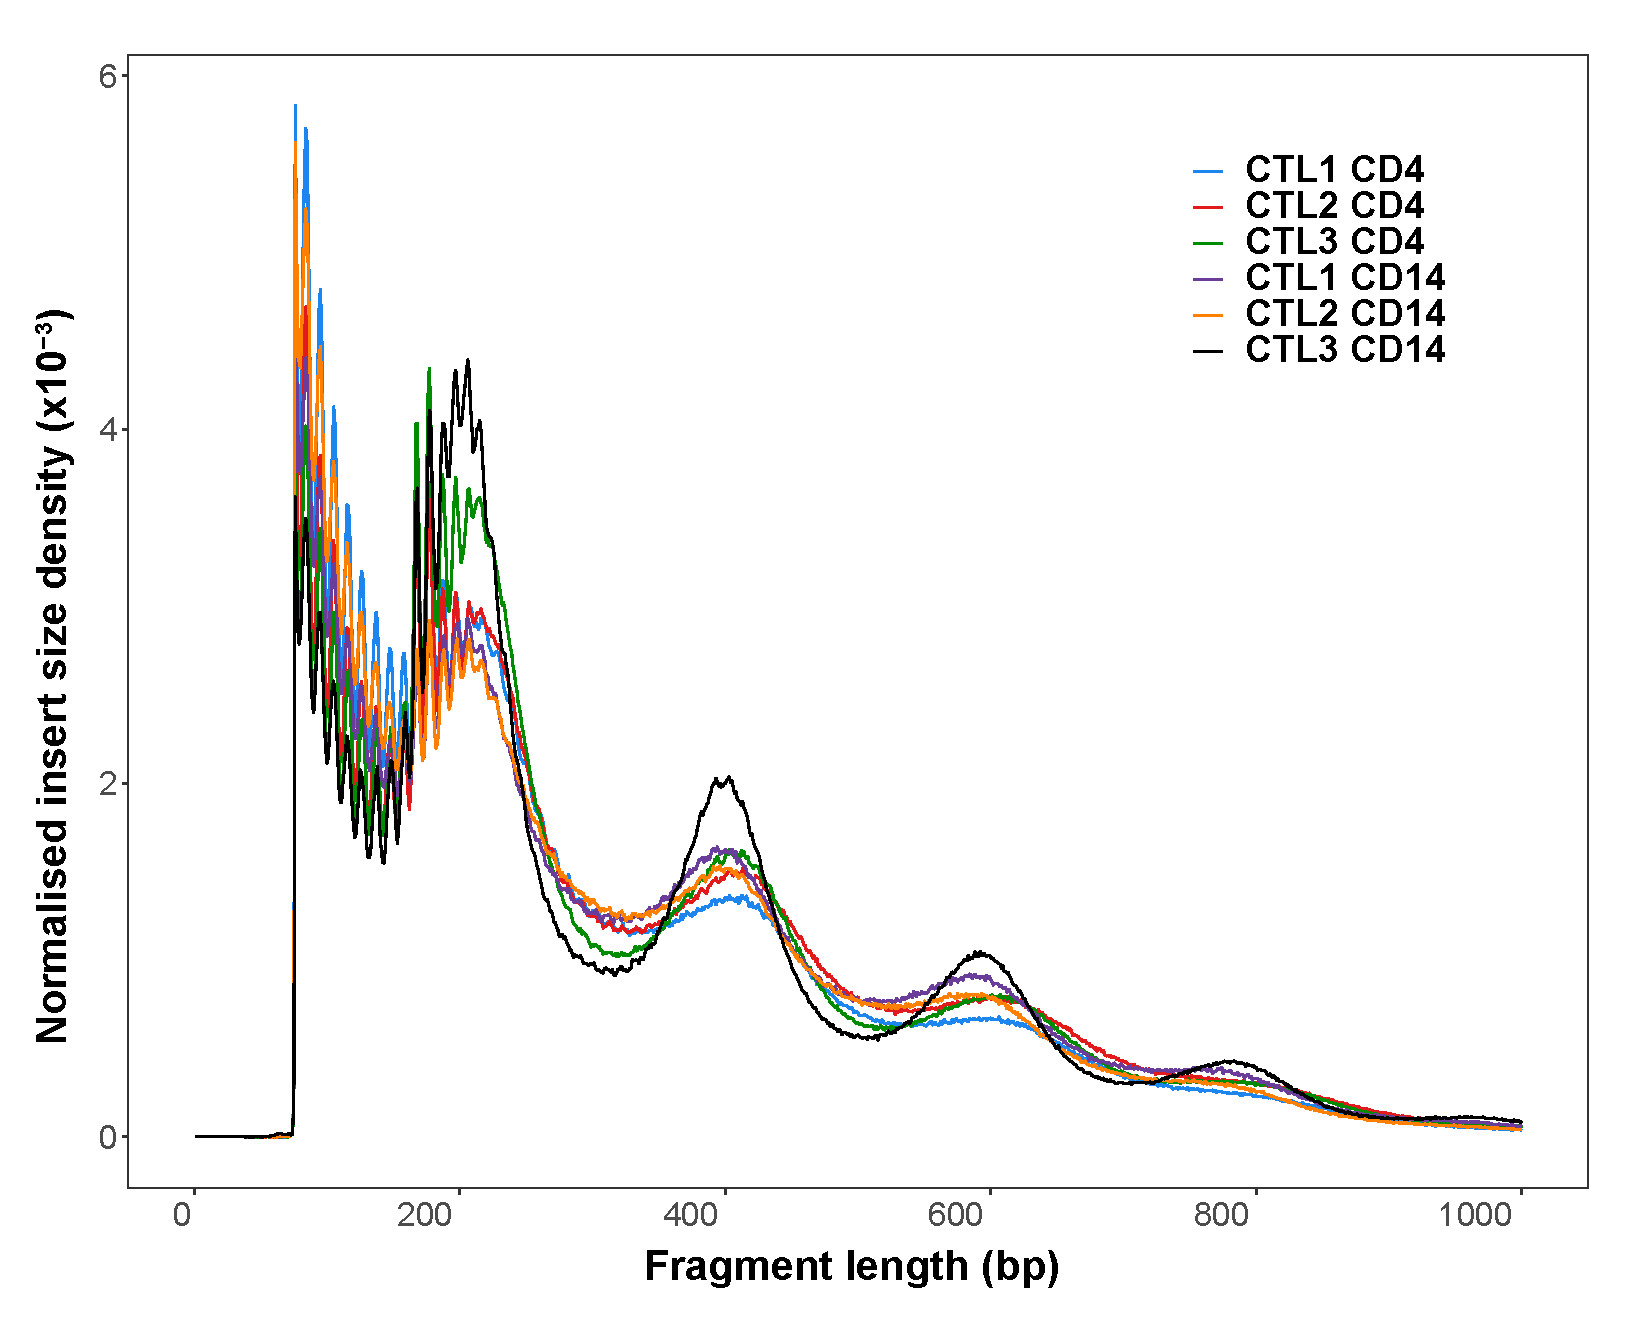
\includegraphics[width=\textwidth]{./Results1/pdfs/ATAC_Core_fresh_CD4_CD14_frag_size_distribution}
\caption{\textbf{}}
\end{subfigure}%
\begin{subfigure}[b]{0.45\textwidth}
\centering
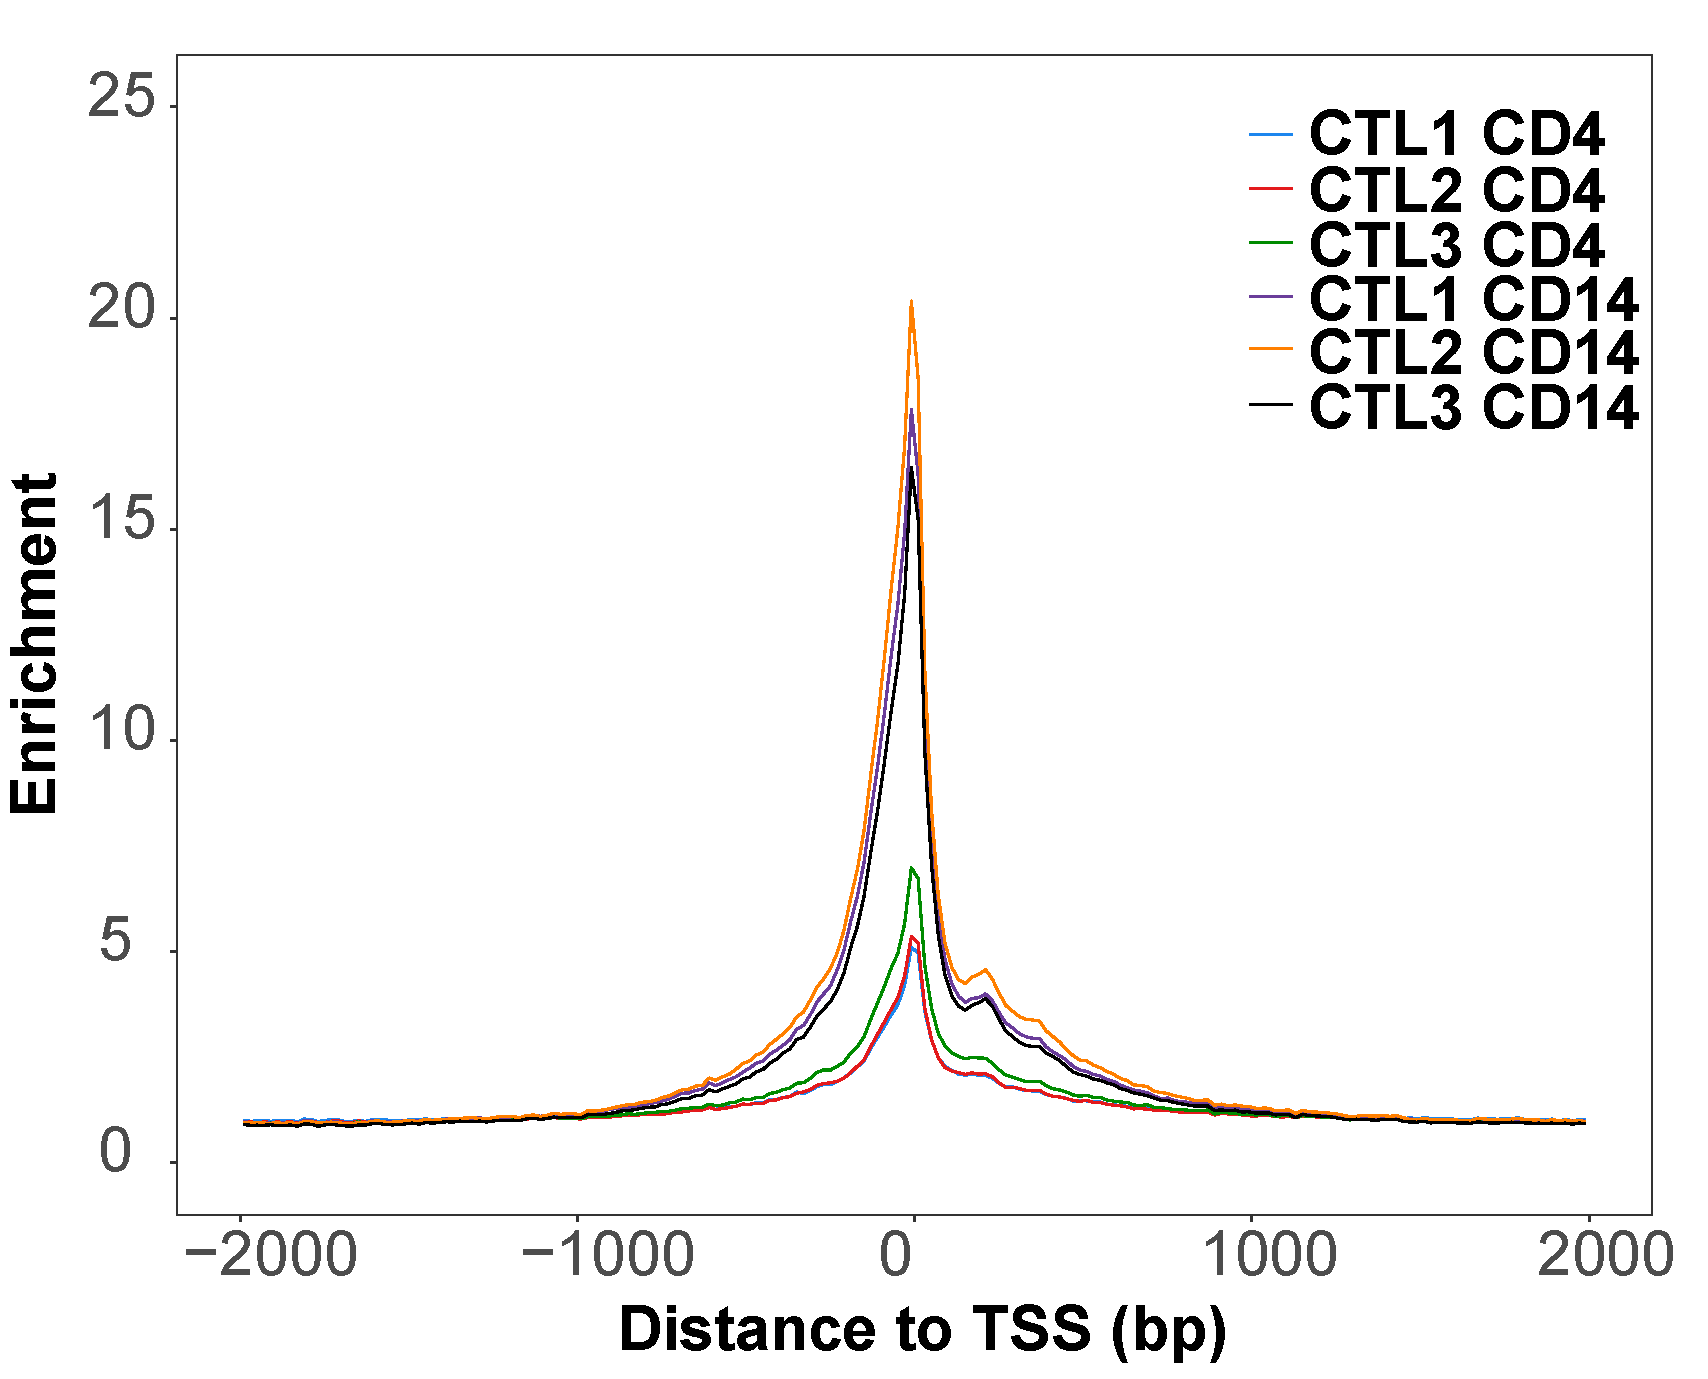
\includegraphics[width=\textwidth]{./Results1/pdfs/TSS_enrichment_Core_fresh_CD4_CD14}
\caption{\textbf{}}
\end{subfigure}
\begin{subfigure}[b]{0.6\textwidth}
\centering
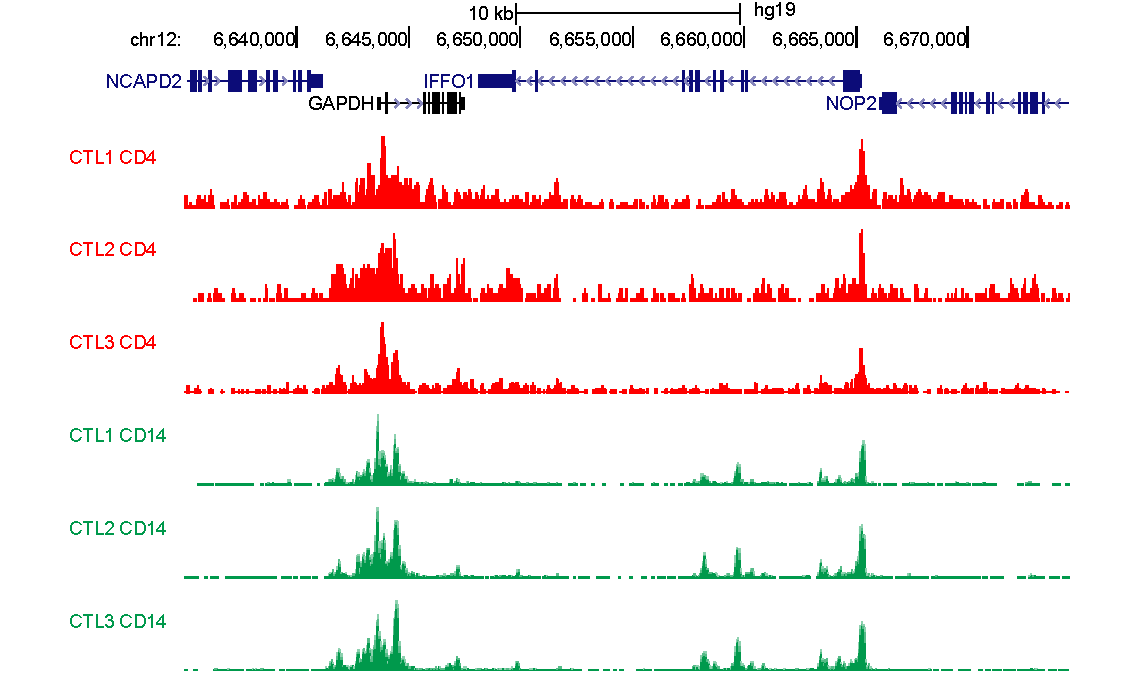
\includegraphics[width=\textwidth]{./Results1/pdfs/ATAC_Core_CD4_CD14_fresh_GAPDH}
\caption{\textbf{}} % to add text to the figure name
\end{subfigure}
\caption[Measurements for quality control assessment in ATAC-seq samples]{\textbf{Measurements for quality control assessment in ATAC-seq samples.} For each of the CD14$^+$ monocytes and CD4$^+$ samples used to establish the ATAC analysis pipeline quality control measures (A) density distribution of ATAC-seq fragment sizes, (B) enrichment of ATAC-seq fragments across the TSS of all Ensembl genes and (C) UCSC Genome Browser view illustrating the ATAC-seq normalised read density (y-axis) at the promoters of \textit{GAPDH} and \textit{NOP2} genes are shown. CD14$^+$ monocytes and CD4$^+$ tracks are colour-coded in green and red, respectively.}
\label{figure:QC_ATAC}
\end{figure} 

Positive correlation between the TSS fold-change enrichment and FRiP was observed and suggested that both are appropriate inter-dependent quality control measures to evaluate sample noise. For the six samples analysed here, mitochondrial content varied between (14.9-43.3\%), was higher in CD14$^+$ than in CD4$^+$ cells and was not directly related to any of the other quality control measurements (Table \ref{tab:ATAC_MT_fraction_reads_in_peaks}). Therefore, mitochondrial reads in this range did not appear to reflect sample quality and the main issue related to the need for deeper sequencing to achieve the desired number of non-mitochondrial reads for downstream analysis.

 

\begin{table}[htbp]
%\setlength{\tabcolsep}{20pt} only to stretch the columns if you want
%\renewcommand{\arraystretch}{1.5}
\centering
\begin{tabular}{@{} c c c}
\toprule
\textbf{Sample} & \textbf{\% mitochondrial reads} & \textbf{Fraction of reads in peaks} \\
\midrule
\midrule
CTL1 CD4 & 14.9 & 9.8 \\
CTL2 CD4 & 30.5 & 11.2 \\
CTL3 CD4 & 28.8 & 11.6 \\
CTL1 CD14 & 43.3 & 32.2 \\
CTL2 CD14 & 36.8 & 57.0 \\
CTL3 CD14 & 37.6 & 49.9 \\
\bottomrule
\end{tabular}
\medskip %gap
\caption[ATAC-seq percentage of mitochondrial reads and fraction of reads in called peaks (FRiP).]{\textbf{ATAC-seq percentage of mitochondrial reads and fraction of reads in called peaks (FRiP).} The percentage of mitochondrial reads was calculated over the total number of sequencing reads (before filtering). FRiP was calculated as the proportion of ATAC-seq fragments overlapping significant peaks with standard filtering for all the samples (FDR$<$0.01).}
\label{tab:ATAC_MT_fraction_reads_in_peaks}
\end{table}



Both TSS and FRiP are appropriate signal-to-noise measures, being the recommended threshold values by ENCODE and Alasoo \textit{et al.} 2018 (previously published in bioRxiv in 2017) 10-20\% for FRiP and 6-10 for TSS enrichment. Importantly, ENCODE has recently prioritised the use of TSS over FRiP as a more stable measure to determine noise and therefore this was the chosen measure for this thesis. In summary from this analysis, all six samples showed appropriate ATAC-seq patterns of fragment size distribution, FRiP and TSS, with the exception of CD4$^+$ CTL1 and CTL2, being borderline for the 6 fold-enrichment ENCODE TSS recommended threshold.
%Importantly, this differences in the enrichment around the TSS successfully recapitulated the differences observed in the ATAC-seq density signal of the UCSC Genome Browser tracks between the CD14$^+$ and CD4$^+$ samples. These differences in ATAC-seq quality observed in these samples reflected the variability in performance of ATAC-seq and were useful in determining the influence of borderline sample quality in downstream analysis in order to choose the most robust strategy maximising the use of precious clinical samples. 



\subsubsection{Peak calling and filtering}
\label{peak_filtering}
Next, criteria for peak calling and filtering were investigated. Although different peak callers have been used to analyse ATAC-seq data, MACS2 has been the preferred algorithm by ENCODE and most publications at the time of this thesis (Table \ref{tab:ATAC_comparative_methods}). MACS2 was initially developed for ChIP data, but has also been used for DHS and ATAC-seq disabling the model option and manually setting the shift (--shift) and extension size (--extsize) parameters, which refer to the number of bp and direction for the reads to be shifted and the number of bp for them to be extended, respectively. Since the --extsize should correspond to the average fragment size, this was set to 200bp, the average fragment size calculated for the ATAC-seq libraries in this project. The --shift was set to -100, as it is recommended to be -1/2 of the fragment size when analysing chromatin accessibility data so that the summit of the peak is located at the Tn5 insertion site. 

A systematic analysis of the effect of sequencing depth and the sample quality on peak calling was conducted to better understand the effect of both variables on the downstream analysis. For each of the six samples, random sub-sampling of reads was performed in every 5 million increment, ranging from 5 to 30 total million reads, followed by peak calling with arbitrary filtering for false discovery rate (FDR)$<$0.01. The number of called peaks passing filtering showed a steady increase with read depth  (Figure \ref{figure:Peak_calling_versus_depth_ATAC}A), beginning to plateau at approximately 25 million reads (Figure \ref{figure:Peak_calling_versus_depth_ATAC}B). Moreover, lower number of peaks were detected in CD4$^+$ samples compared to CD14$^+$ monocytes when using standard  FDR$<$0.01 filtering, highlighting the influence of sample quality on the total number of called peaks. Interestingly, sample quality as measured by FRiP (which relies on peak calling) showed very small changes with read depth and was stable from 15 million reads onwards for all six samples (Figure \ref{figure:Peak_calling_versus_depth_ATAC}C), similarly to TSS (Figure \ref{figure:Peak_calling_versus_depth_ATAC}D). This confirmed that measurement of sample quality using FRiP or TSS was not affected by the sequencing depth.

\begin{figure}[H]
\centering
\begin{subfigure}{0.48\textwidth}
\centering
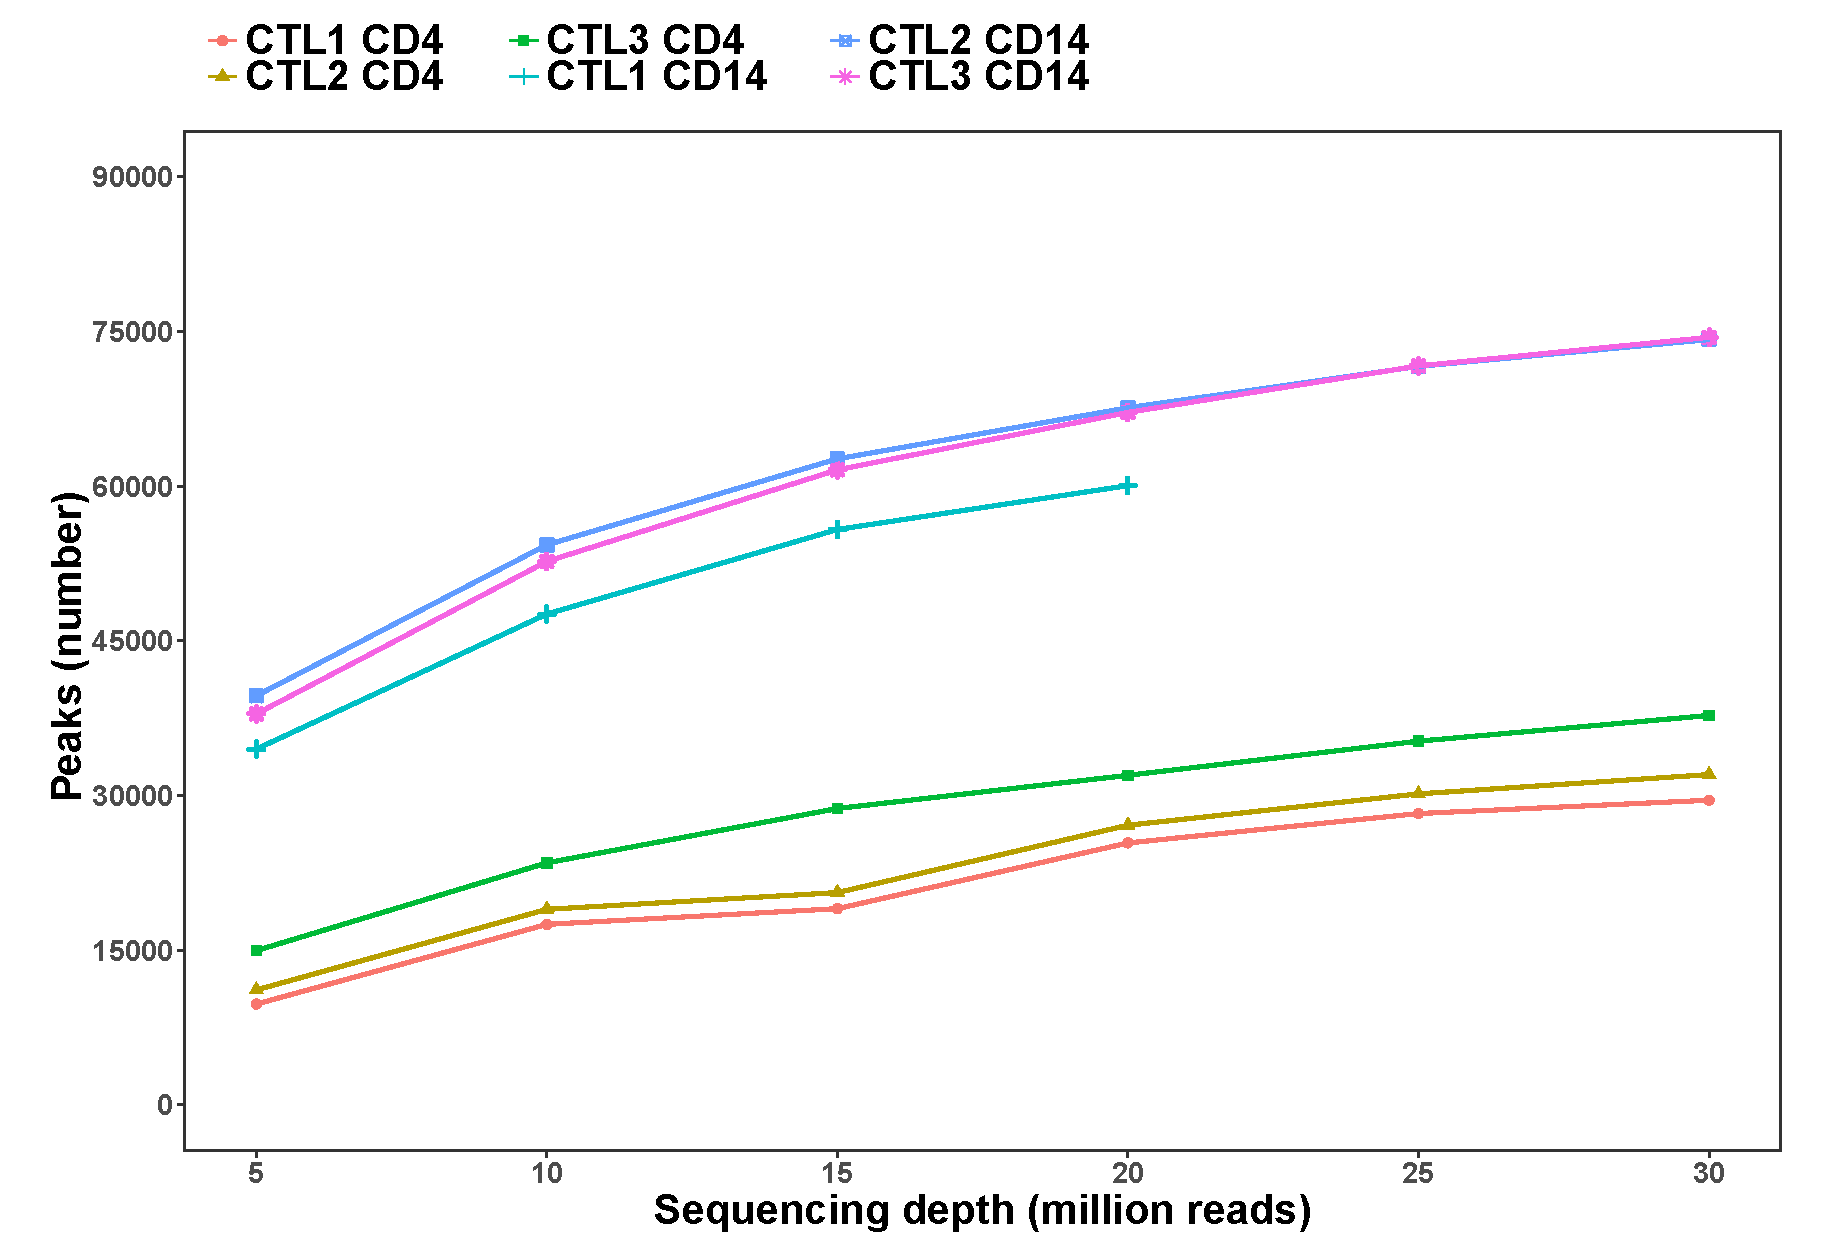
\includegraphics[width=\textwidth]{./Results1/pdfs/ATAC_Core_fresh_CD4_CD14_num_peaks_vs_depth}
\caption{\textbf{}}
% The percentage sign indicated that the other subfig goes side by side
\end{subfigure} %
\begin{subfigure}{0.48\textwidth}
\centering
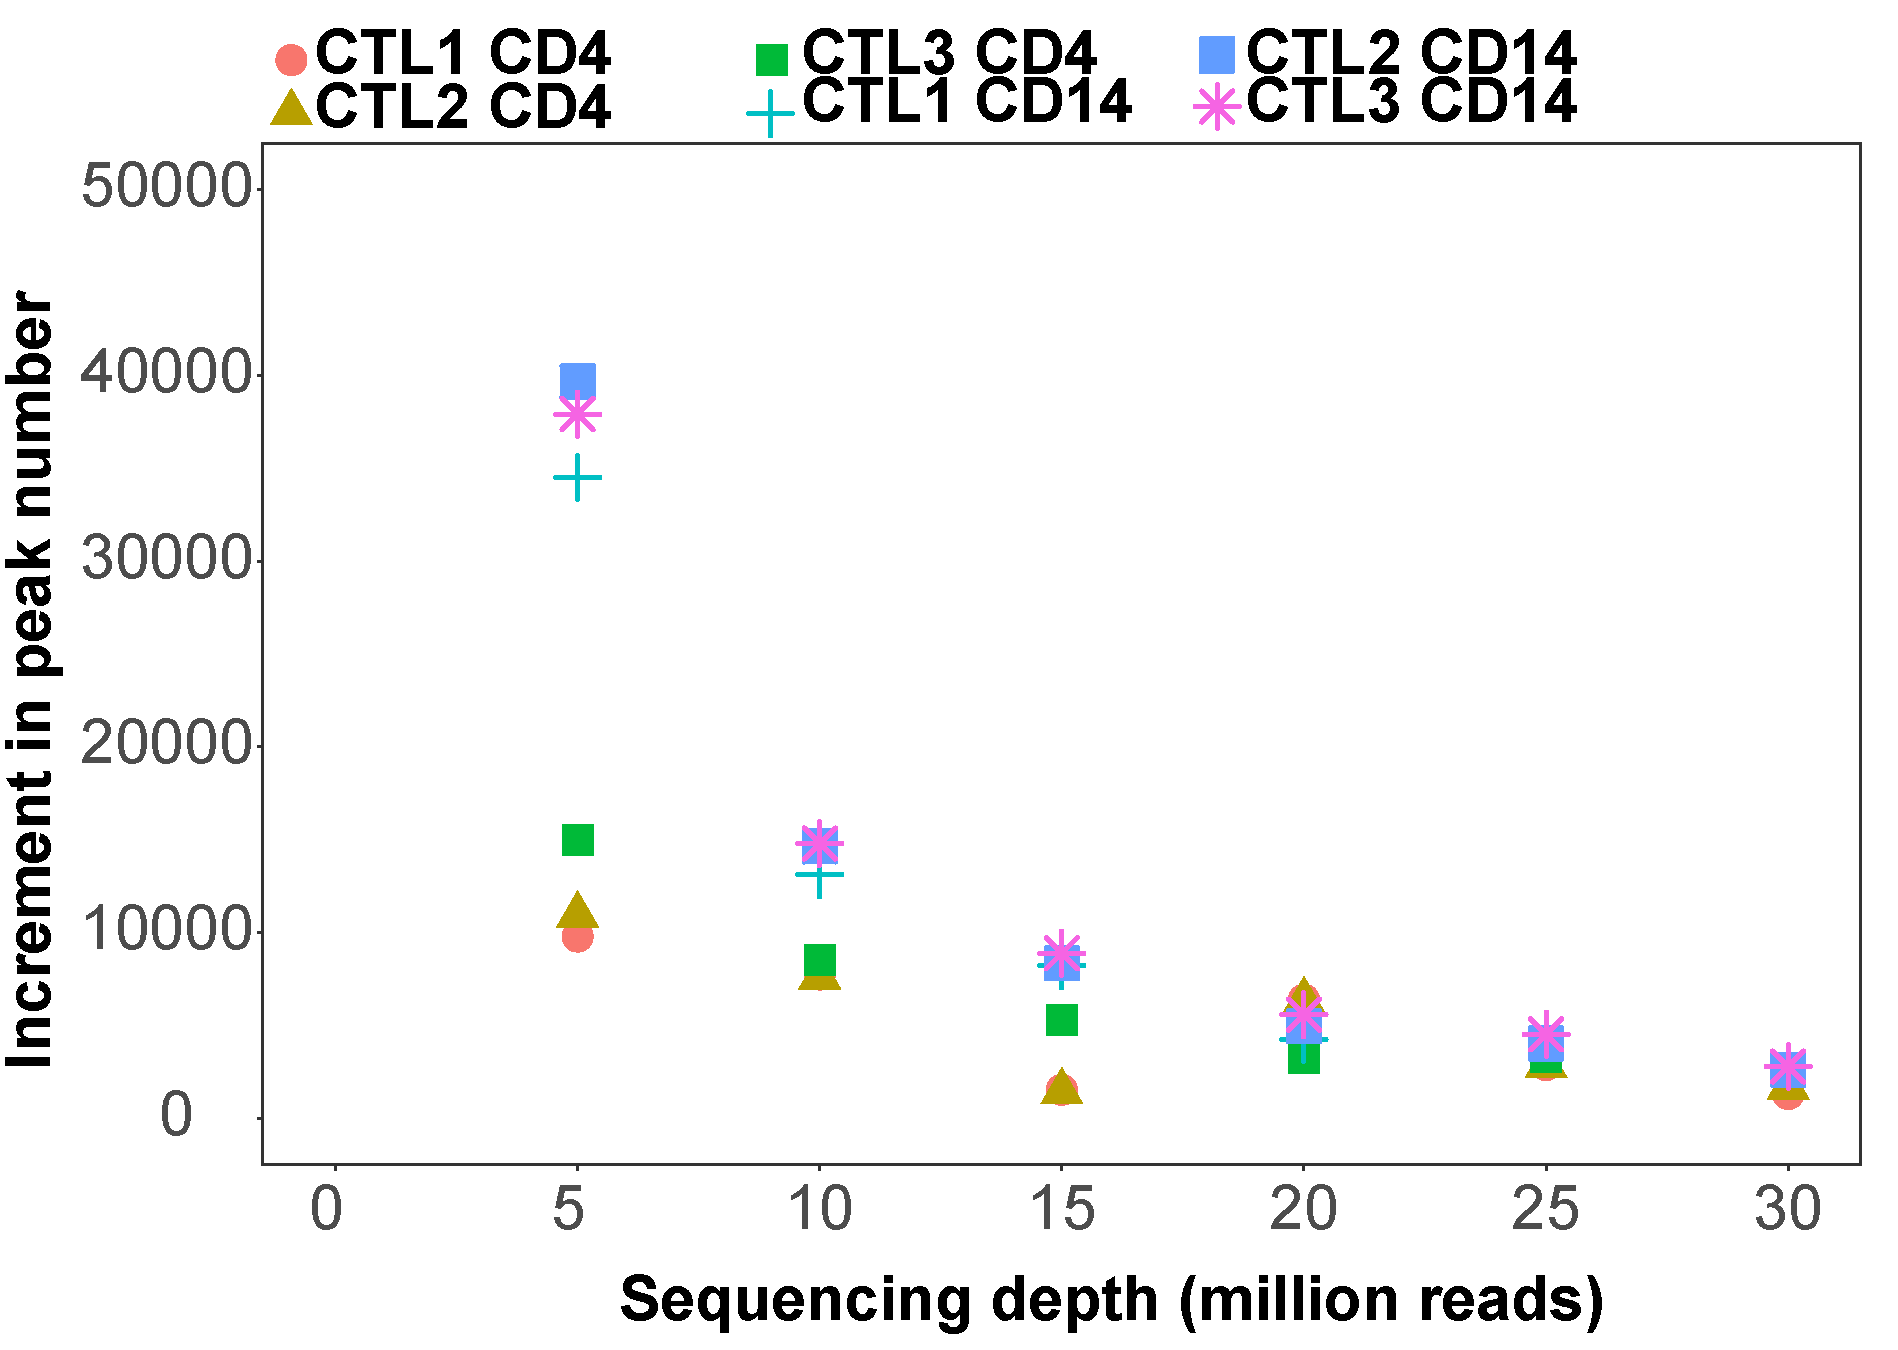
\includegraphics[width=\textwidth]{./Results1/pdfs/ATAC_Core_fresh_CD4_CD14_increment_num_peaks_vs_depth}
\caption{\textbf{}}
\end{subfigure} 
\begin{subfigure}{0.48\textwidth}
\centering
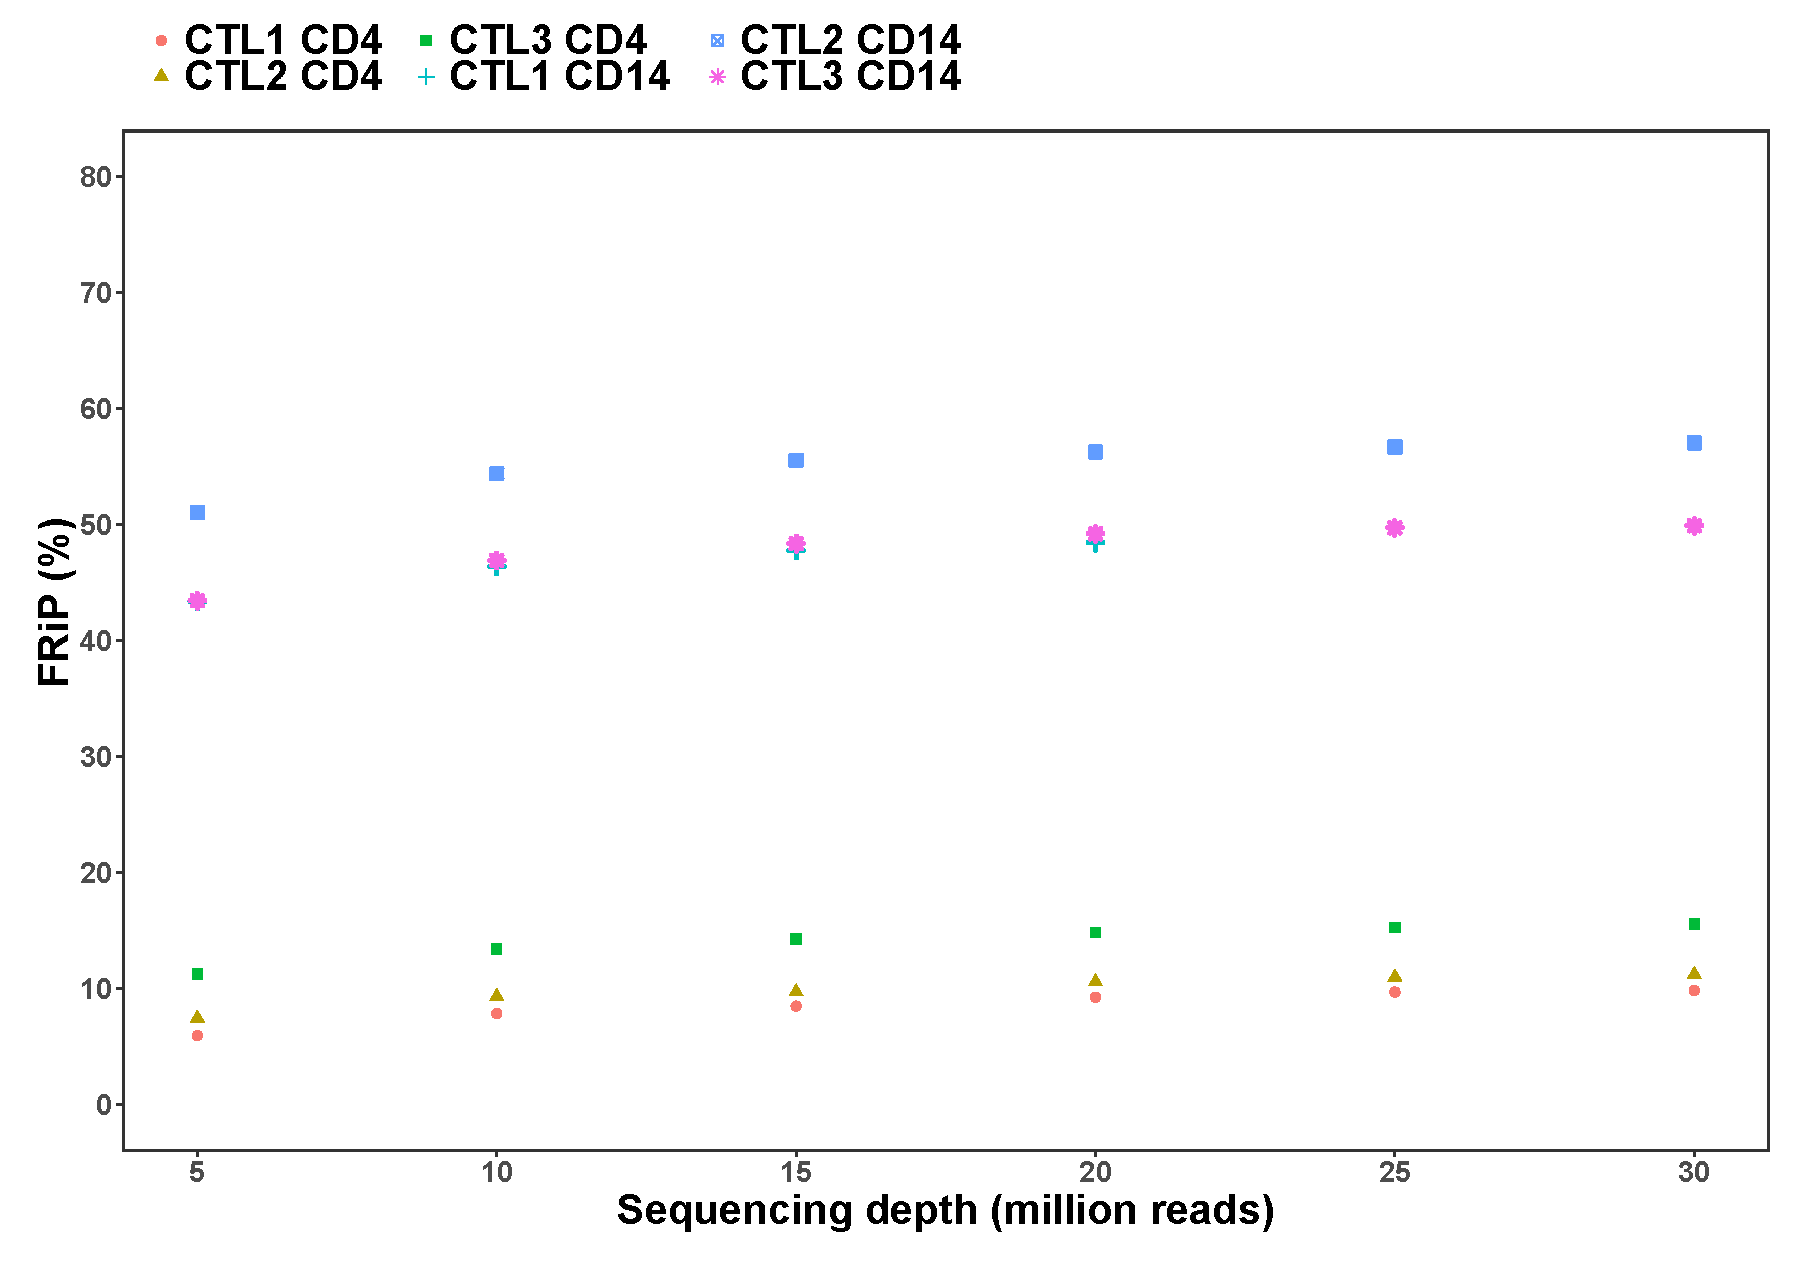
\includegraphics[width=\textwidth]{./Results1/pdfs/ATAC_Core_fresh_CD4_CD14_frac_reads_in_peaks_vs_depth}
\caption{\textbf{}}
\end{subfigure}%
\begin{subfigure}{0.48\textwidth}
	\centering
	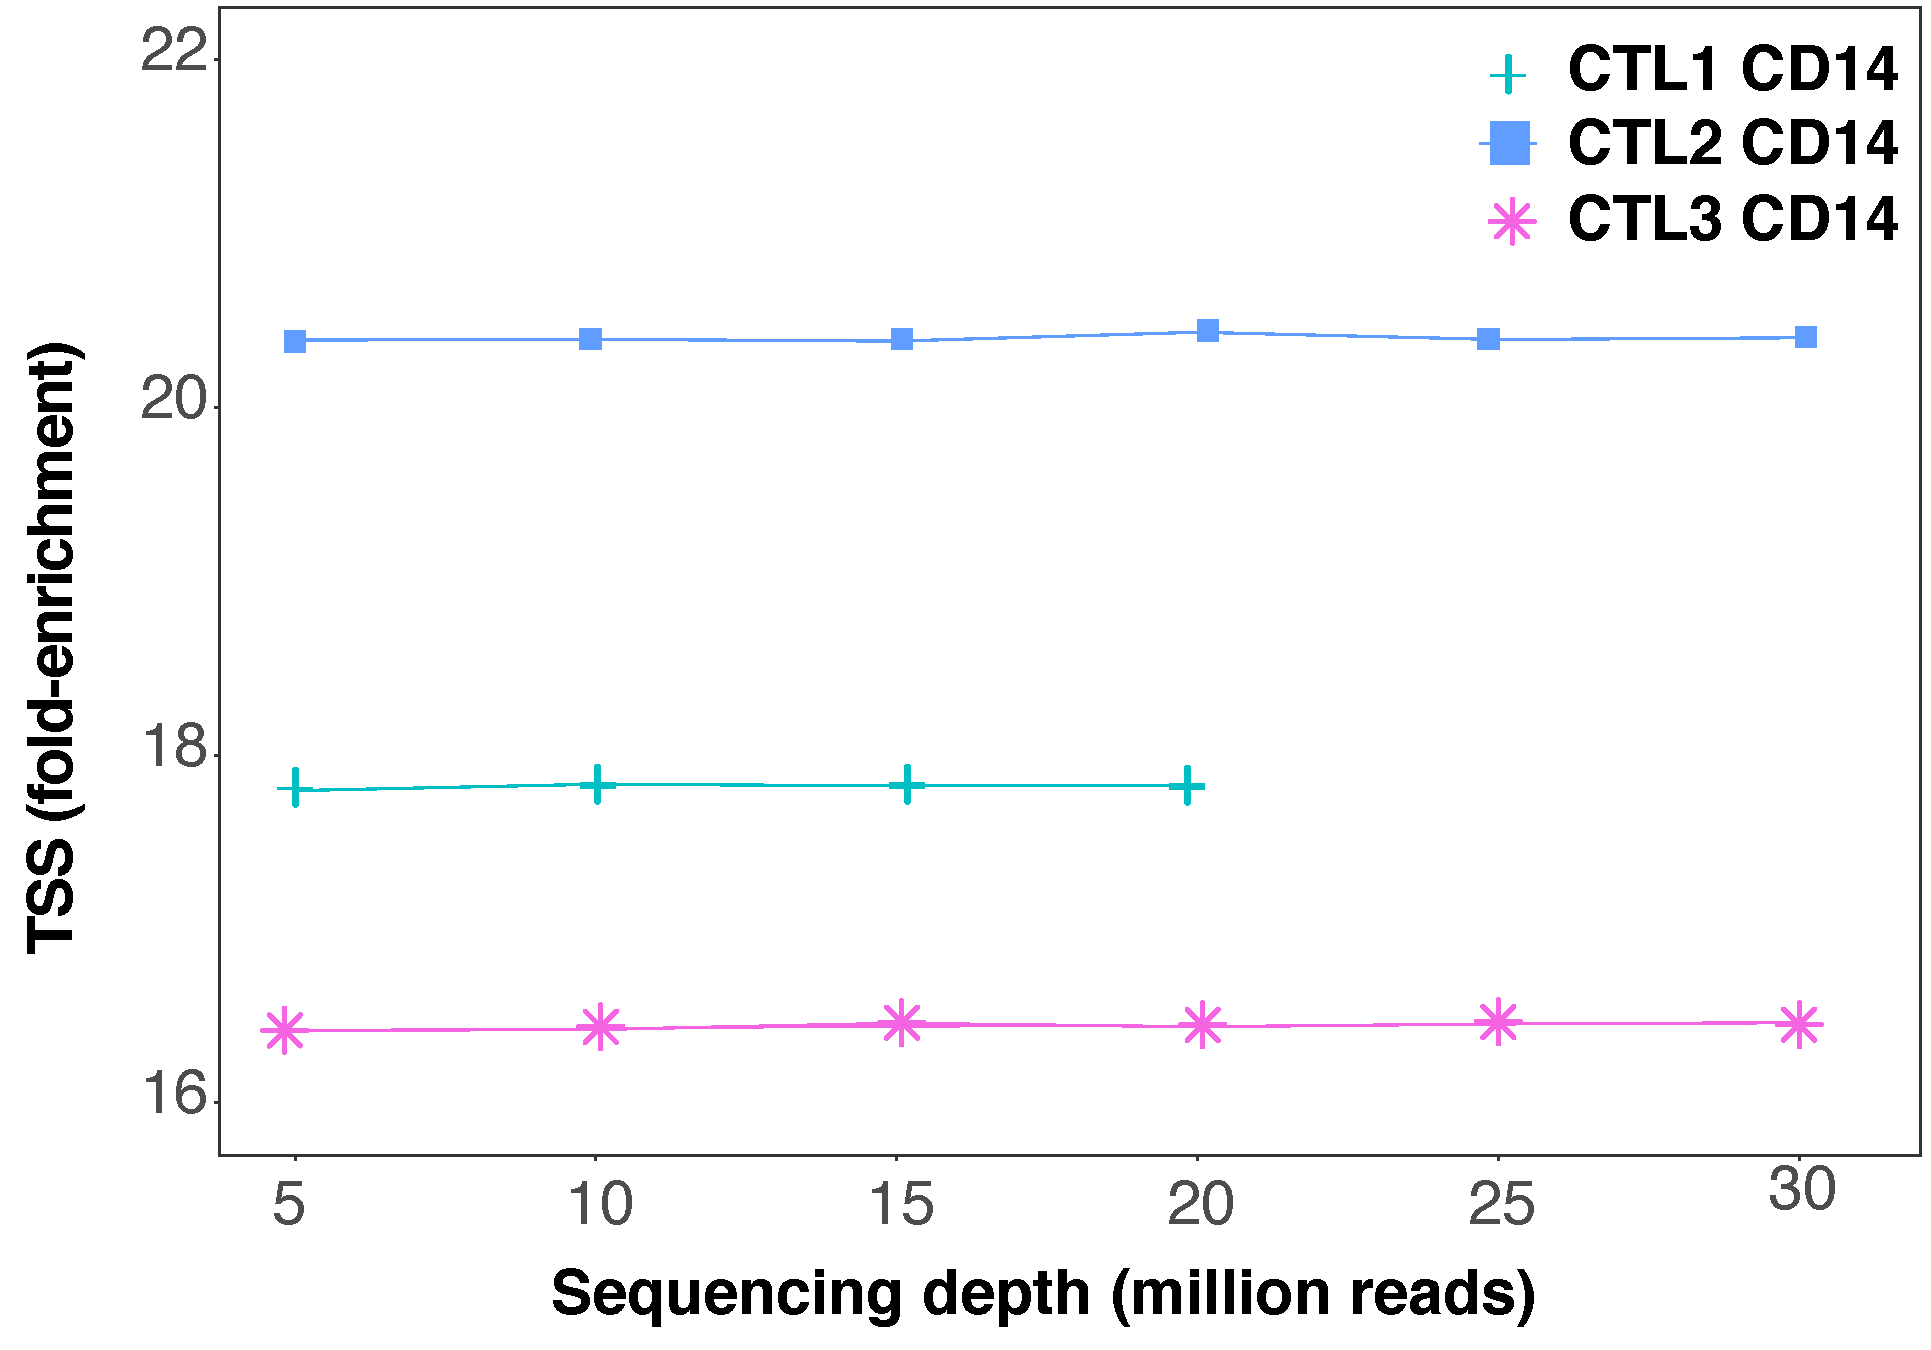
\includegraphics[width=\textwidth]{./Results1/pdfs/Core_TSS_vs_sequencing_depth_CD14}
	\caption{\textbf{}}
\end{subfigure}
\caption[FRiP and peak calling at different sequencing depths in ATAC-seq libraries.]{\textbf{FRiP and peak calling at different sequencing depths in ATAC-seq libraries.} For a series of sequencing depths (from 5 to 30 million reads after filtering) representation of (A) number of called peaks (standard filtering using FDR$<$0.01, (B) the increment on the number of called peaks and (C) FRiP and (D) TSS as a function of the sequencing coverage in CD4$^+$ and/or CD14$^+$ samples.}
\label{figure:Peak_calling_versus_depth_ATAC}
\end{figure} 


For peak filtering, an arbitrary FDR$<$0.01 in MACS2 is typically used (Table \ref{tab:ATAC_comparative_methods}) but may not remove low quality peaks equally successfully in lower quality samples and does not take into account the reproducibility of the called peaks. Thus IDR was used to experimentally identify the most appropriate p-value threshold to filter the called peaks in each individual sample. Filtered reads from each sample were partitioned in half to create two pseudoreplicates, peaks were called in each pseudoreplicate and the percentage of peaks sharing IDR rank position when filtered at decreasing p-values was calculated (Figure \ref{figure:Peak_calling_IDR_filtering_and_chrom_stated_ATAC}A and B). This strategy was tested across a range of total read counts (as above) to determine the effect of sequencing depth on the suitability of this peak calling filtering approach. The optimal p-value giving the largest percentage of IDR shared peaks between the two pseudoreplicates varied more erratically when the sequencing depth was lower than 10 million reads (Figure \ref{figure:Peak_calling_IDR_filtering_and_chrom_stated_ATAC}A and B), suggesting this analysis was not appropriate for lower read depths. This variation was more pronounced and extended in CD4$^+$ T cells, which had lower TSS values compared to CD14$^+$ monocytes (Figure \ref{figure:Peak_calling_IDR_filtering_and_chrom_stated_ATAC}A and B). The shape of the curves were also influenced by the sample quality. For appropriate sequencing depth (minimum of 15-20 million reads), the CD14$^+$ monocytes (TSS enrichment $\geq$10) samples presented a profile reaching a single maximum of shared IDR peaks for a particular filtering p-value (Figure \ref{figure:Peak_calling_IDR_filtering_and_chrom_stated_ATAC}B), which was -log10 p-value 8 in all three samples (data not shown). In contrast, the same analysis in CD4$^+$ samples reached two local maxima (Figure \ref{figure:Peak_calling_IDR_filtering_and_chrom_stated_ATAC}A). 



\begin{figure}[htbp]
\centering
\begin{subfigure}{0.50\textwidth}
\centering
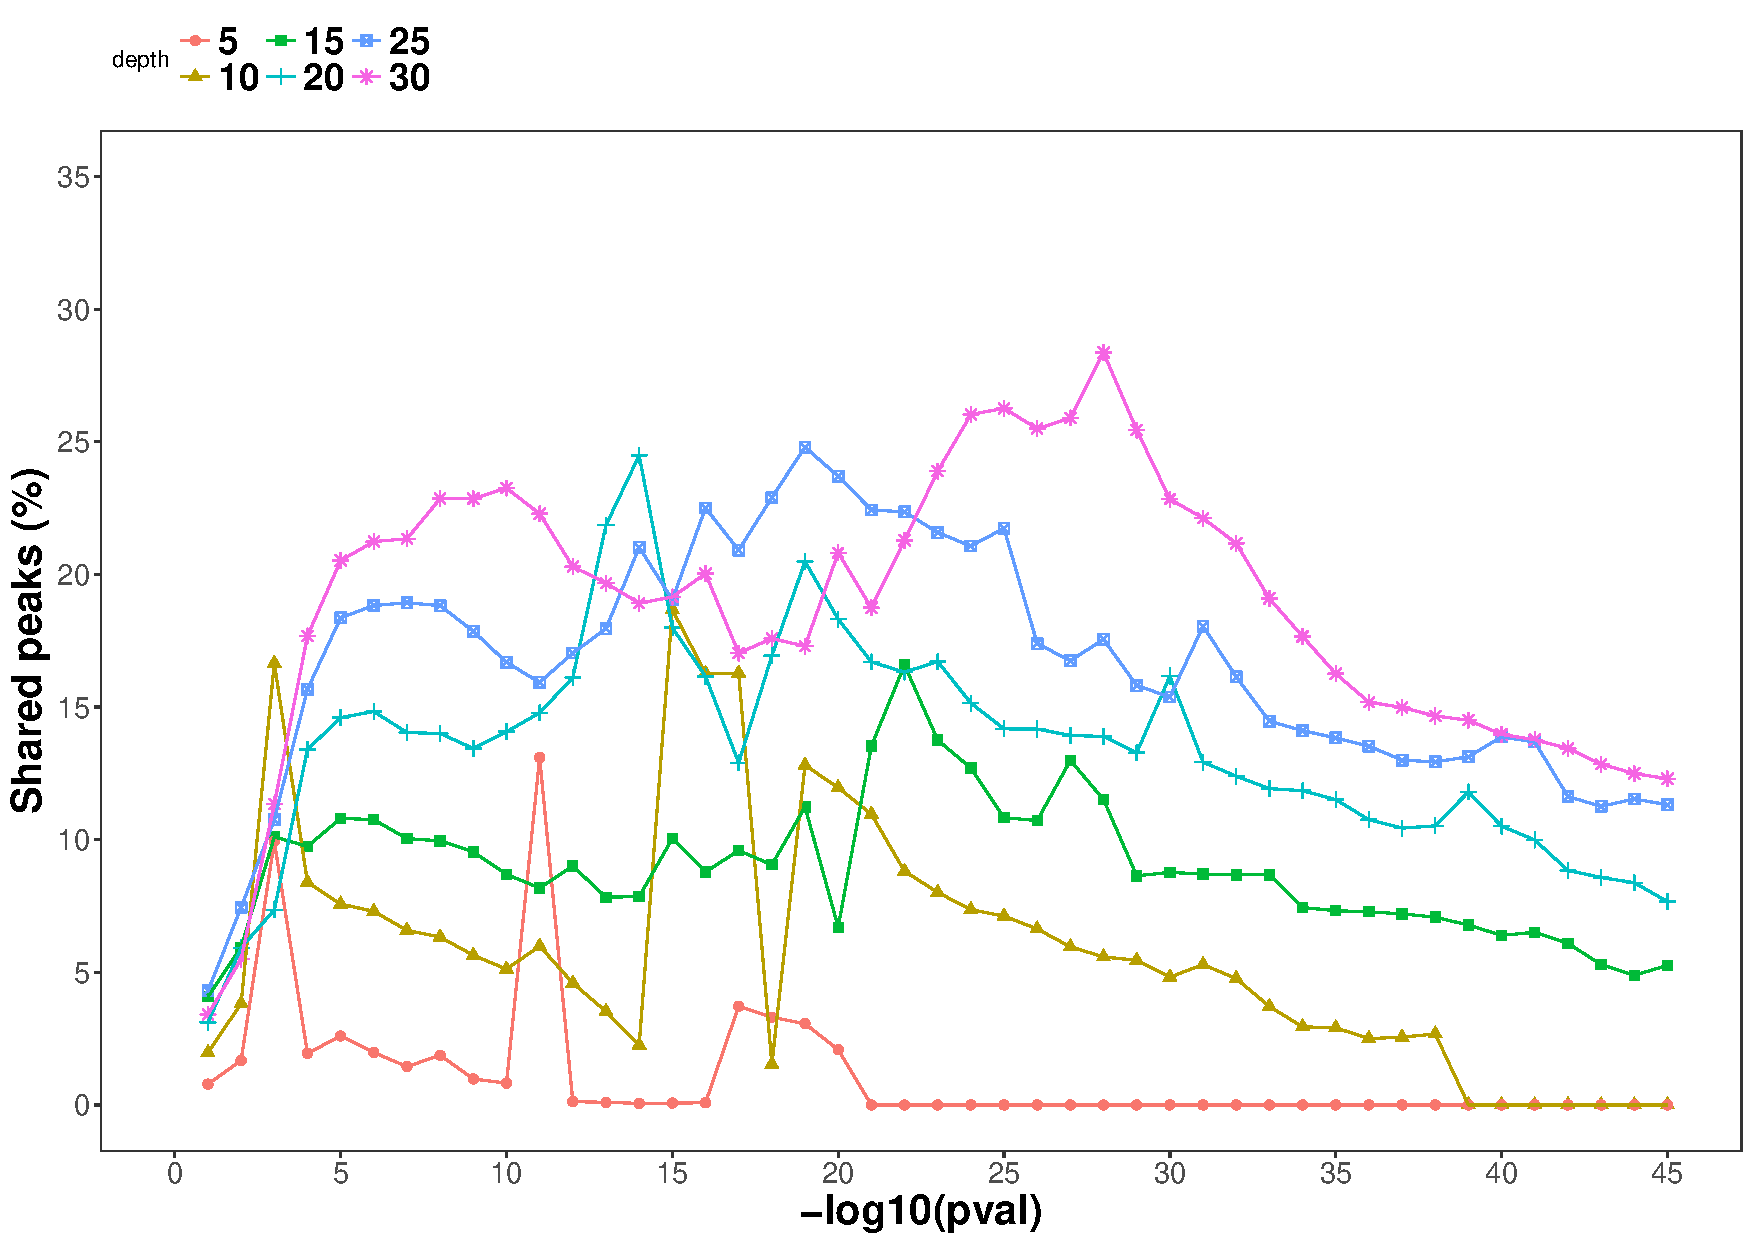
\includegraphics[width=\textwidth]{./Results1/pdfs/ATAC_Core_fresh_CTL2_CD4_shared_peaks_IDR_vs_pval}
\caption{\textbf{}}
% The percentage sign indicated that the other subfig goes side by side
\end{subfigure}%
\begin{subfigure}{0.50\textwidth}
\centering
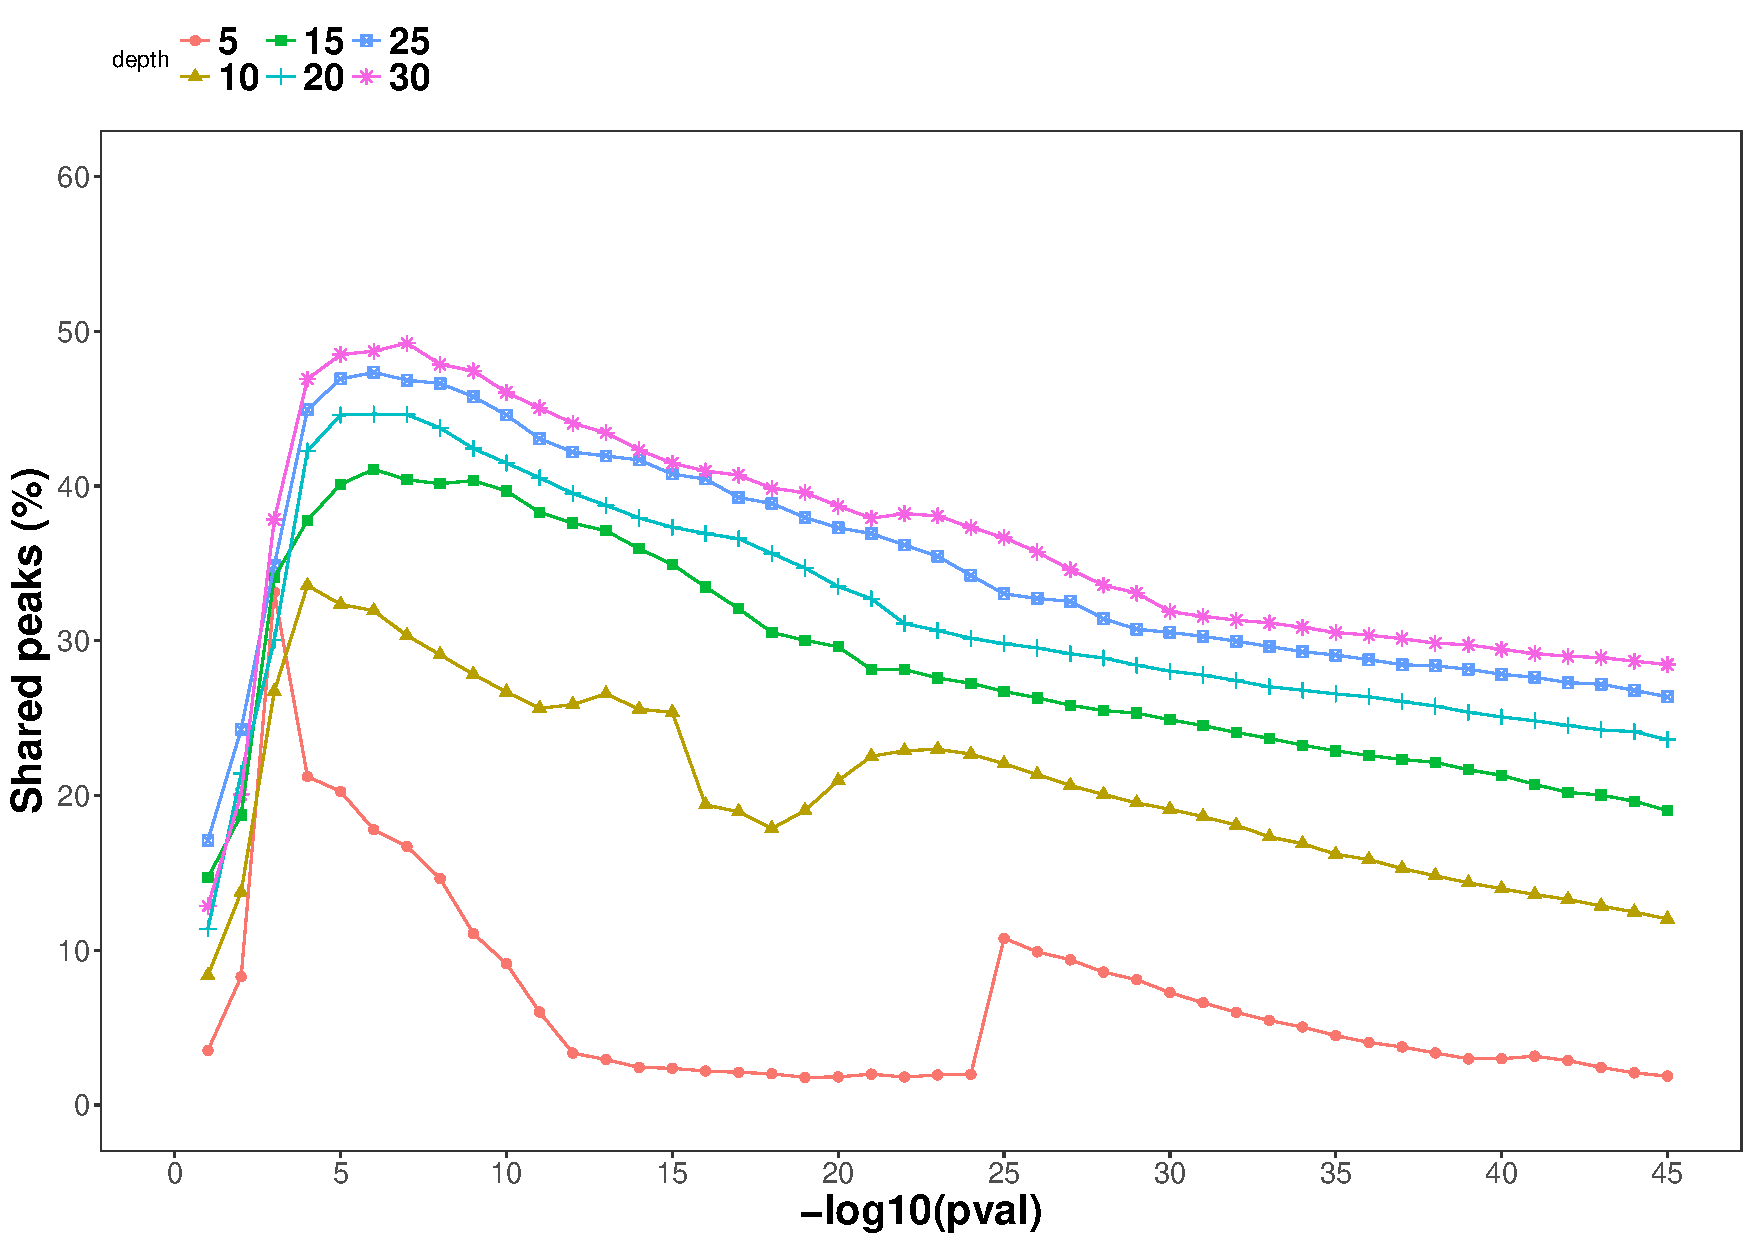
\includegraphics[width=\textwidth]{./Results1/pdfs/ATAC_Core_fresh_CTL2_CD14_shared_peaks_IDR_vs_pval}
\caption{\textbf{}}
\end{subfigure} \\
\begin{subfigure}{0.65\textwidth}
\centering
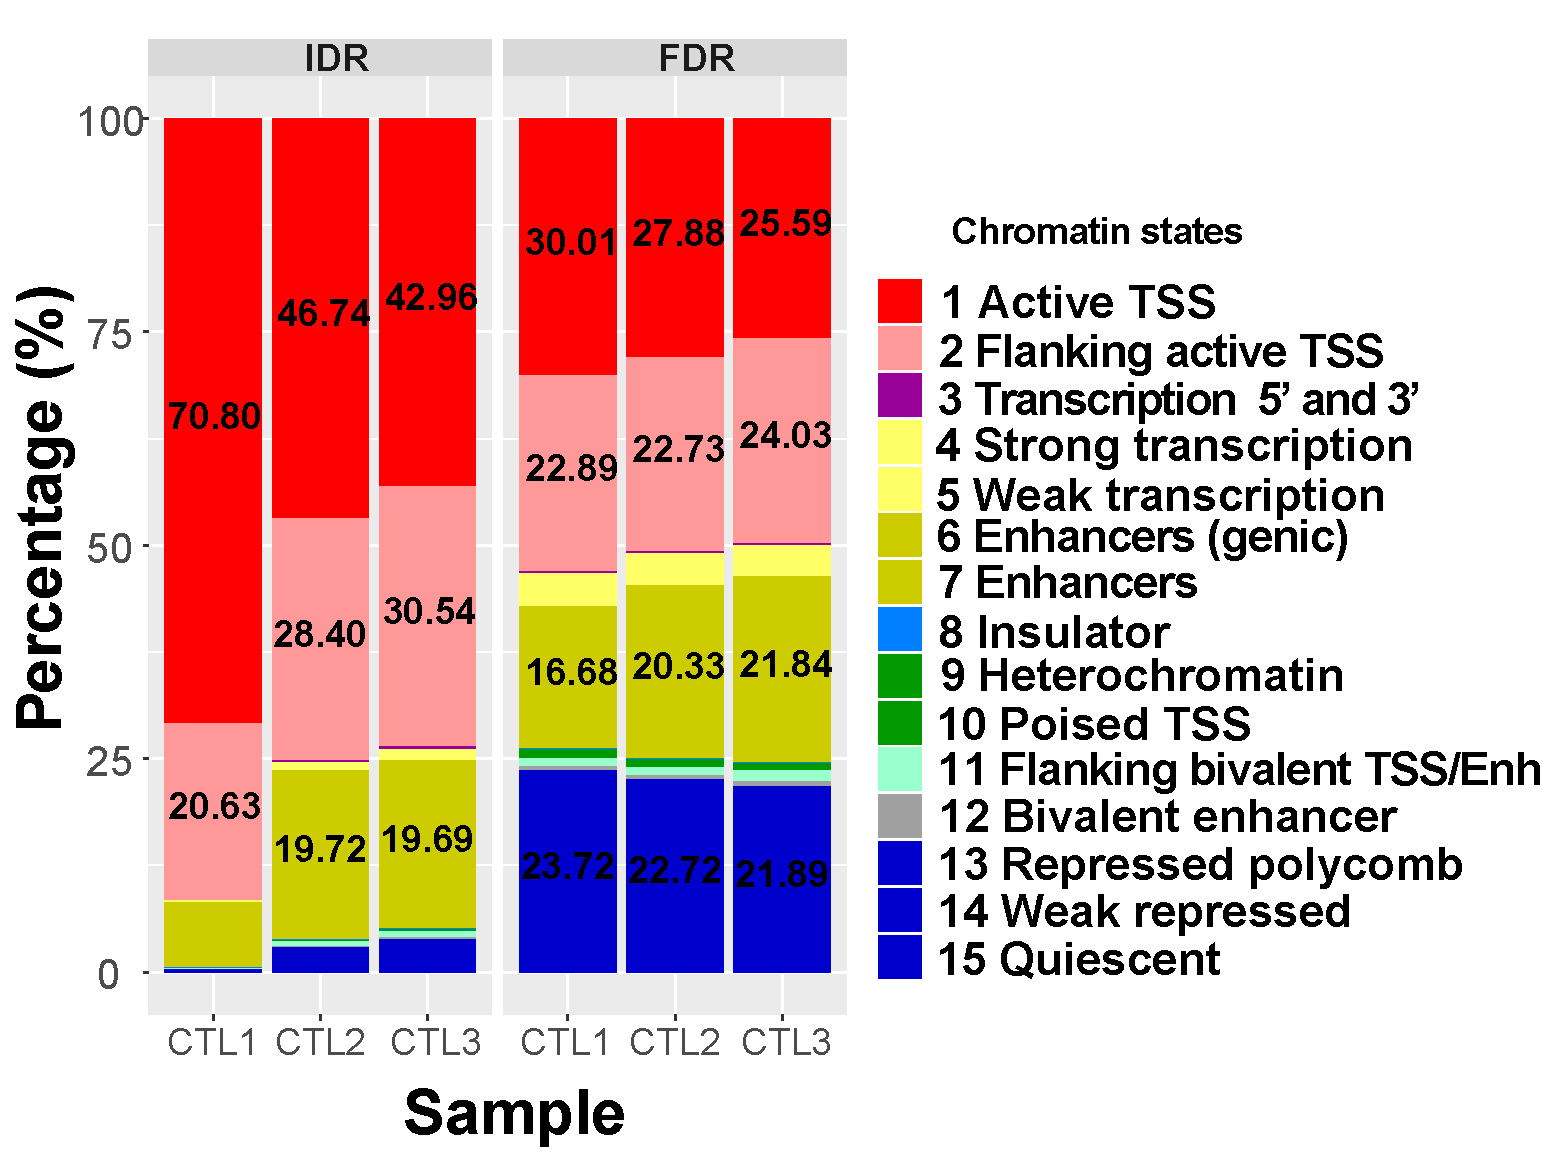
\includegraphics[width=\textwidth]{./Results1/pdfs/stacked_barplot_chromatin_states_percent_CD4_qval_vs_PVAL_IDR_filtered}
\caption{\textbf{}} % to add text to the figure name
\end{subfigure}%
\caption[Peak calling filtering using IDR analysis in ATAC-seq samples.]{\textbf{Peak calling filtering using IDR analysis in ATAC-seq samples.} \ToDo{For each of the sequencing depths tested (from 5 to 30 million reads after filtering), an illustration of the percentage of peaks sharing IDR rank between the two pseudoreplicates is shown when using different p-value filtering thresholds in CTL2 (A) CD4$^+$  T cells and (B) CD14$^+$ monocytes, two representative samples differing in quality for this analysis.}(C) Annotation (as percentage of total) of the CTL1, CTL2 and CTL3 CD4$^+$ ATAC-seq peaks filtered for FDR$<$0.01 or optimal p-value from the IDR analysis (p-value=10$^{-11}$) with the corresponding cell-type specific Roadmap Epigenomics Project chromatin segmentation map.}
\label{figure:Peak_calling_IDR_filtering_and_chrom_stated_ATAC}
\end{figure} 


Filtering the CD4$^+$ peaks at the p-value of the first local maximum (10$^{-11}$) reduced the percentage of peaks overlapping regions suggestive of noise (e.g repressed and quiescent), and increased the proportion of accessible regions located at active TSS when compared to using the list of significant peaks filtered based on FDR$<$0.01 (Figure \ref{figure:Peak_calling_IDR_filtering_and_chrom_stated_ATAC}C). In summary, this IDR analysis provided a systematic method to identify an optimum p-value with which to perform sample-specific filtering of technically reproducible peaks when the sequencing depth was over 10 million reads. These resulting filtered peaks will be used downstream to build the consensus list of ATAC peaks across all the samples and perform differential chromatin accessibility analysis. 

%Should mention that the median of all this first max are used to perform filtering for all the samples because following other pipelines they always use same filtering value for all samples so we need to be consistent across samples


\subsubsection{Differential chromatin accessibility analysis}

A peak-based approach using the number of reads overlapping the peaks included in the consensus list of ATAC peaks (CP\_all) was implemented to perform differential analysis. One of the main limitations of the ATAC-seq and Fast-ATAC protocols (discussed in Sections \ref{ATACseq} and \ref{Fast_ATAC}) is the background signal. Therefore, an empirical cut-off was identified to minimise the impact of background read counts on the peaks included for the differential analysis \parencite{Xinmin2005,Jonker2014}. Moreover, due to lack of consensus in terms of normalisation and differential analysis methods in ATAC-seq (as reviewed in Table \ref{tab:ATAC_comparative_methods}), two strategies were tested (Figure \ref{figure:ML_workflow}). The first involved quantile normalisation of the read count matrix and differential chromatin accessibility analysis using limma voom lineal model. The second strategy consisted of DESeq2, which performs internal normalisation calculating size factors using median of ratios and differential analysis based on negative binomial distribution.

The CP\_all matrix includes all peaks called significant (present) in at least 30\% of the six samples used in this section (Figure \ref{figure:ML_workflow} Step 1). This consensus list of ATAC peaks can include what may be considered background counts, i.e. reads overlapping regions not considered significant in a particular sample (absent) but called as significant (and therefore present) in other samples. The number of reads overlapping peaks in samples where that peak was not called significant (absent) were used to generate a density distribution plot of the background reads (Figures \ref{figure:ML_workflow} Step 2). From this plot, a sequence of twenty cut-offs was defined, with each value representing the number of counts shown by an increasing percentage of the total absent peaks (Figure \ref{figure:ATAC_absent_peaks_distribution}) and each cut-off (corresponding to a minimum number of mapping reads) was applied to filter out peaks from the CP\_all raw count matrix (not normalised) with values lower than the cut-off in more than three samples (Figure \ref{figure:ML_workflow} Step 3). A filter of three samples was chosen as it corresponds to the smallest number of biological replicates in this particular experimental design and ensures that peaks absent in one condition but not in the other are retained. The resulting reduced matrix of low-noise peaks for each cut-off value was then normalised using quantile or DESeq2 (normalisation using size factors as detailed in Love \textit{et al.} 2014) and used to conduct differential analysis with limma voom or DESeq2, respectively. The results from this were used to determine an appropriate threshold for filtering background reads, as well as to compare the two analytical methods. 


\begin{landscape}
\begin{figure}[htbp]
\centering
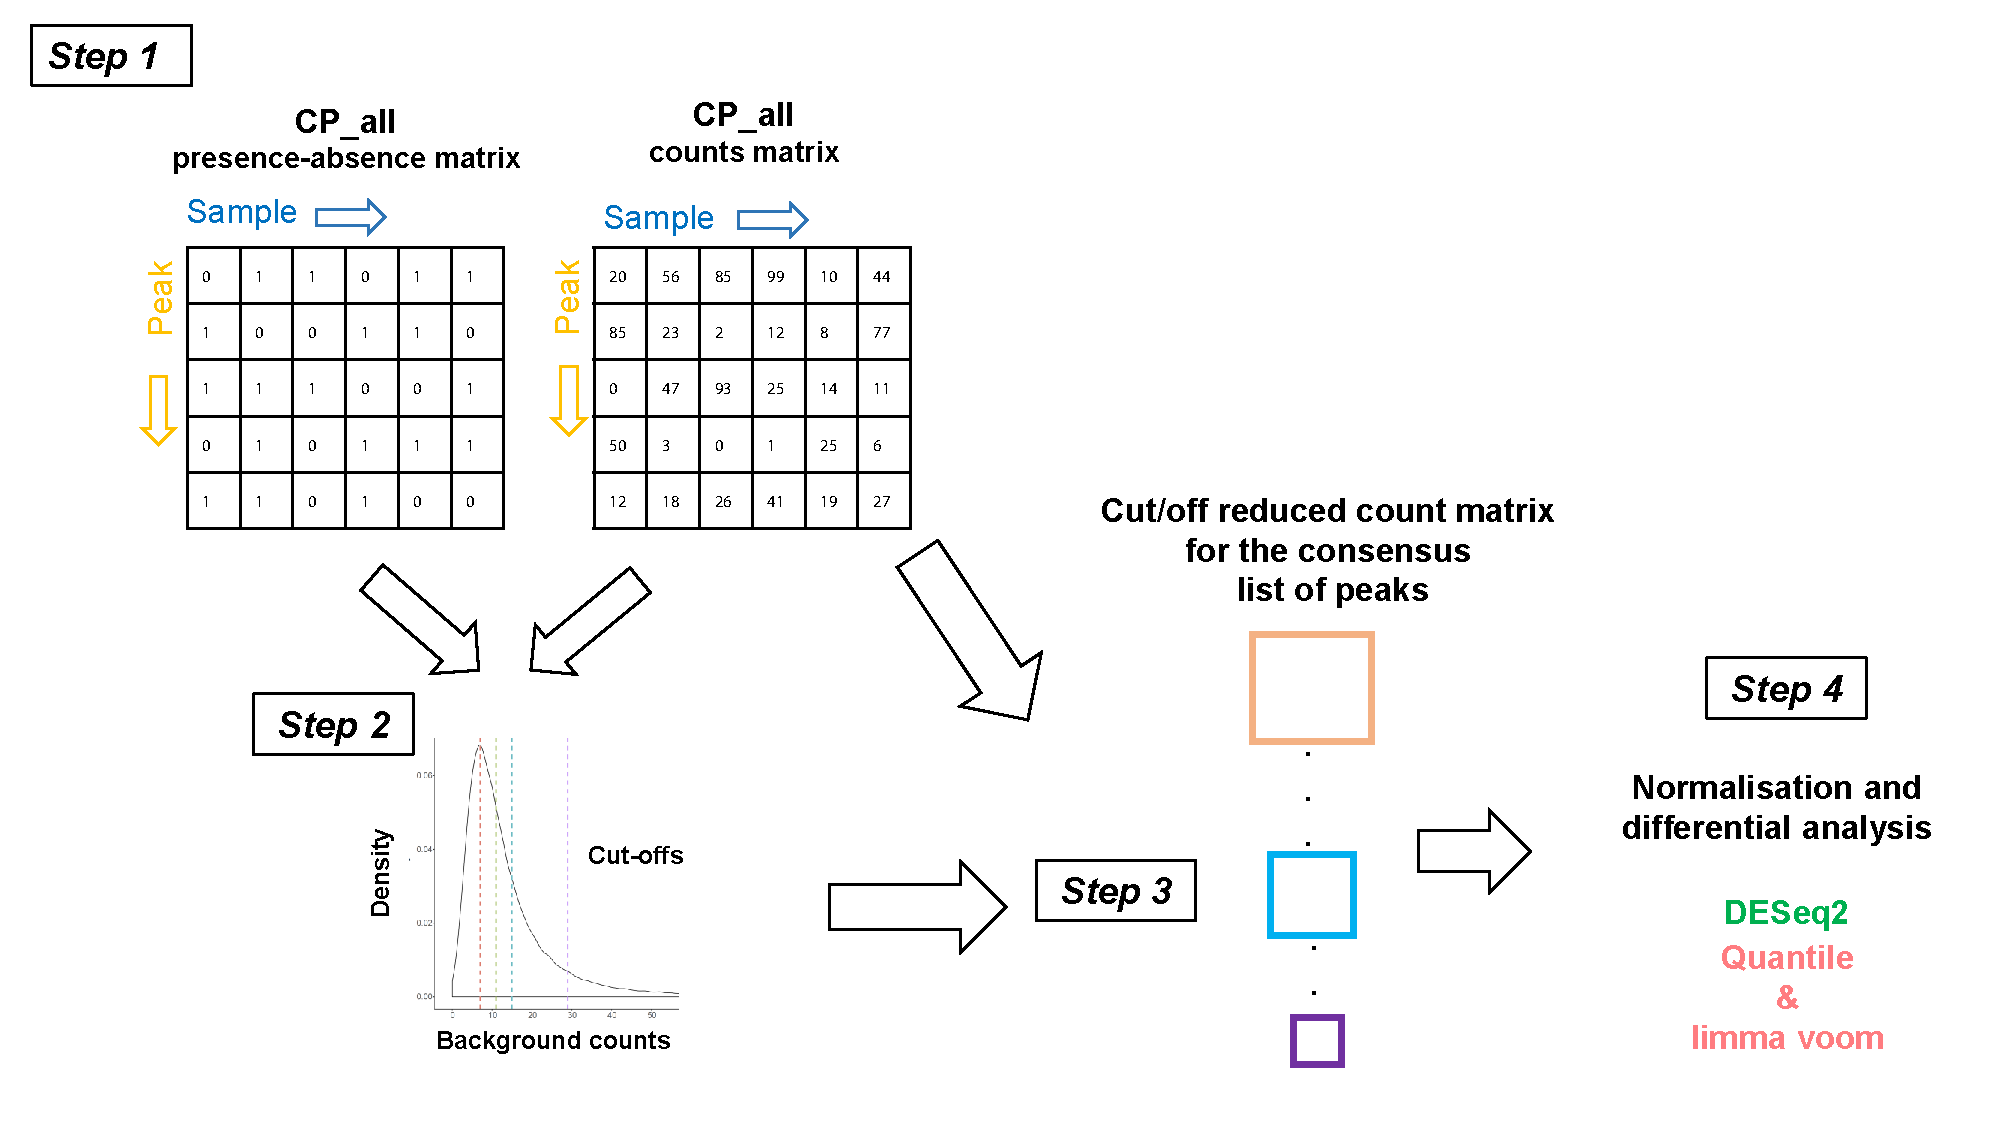
\includegraphics[width=1.2\textwidth]{./Results1/pdfs/ATAC_master_list_filtering_flow_chart}
\caption[Work flow illustrating the strategy to account for ATAC background noise prior to differential analysis.]{\textbf{Work flow illustrating the strategy to account for ATAC background noise prior to differential analysis.} A combined consensus list of ATAC peaks (CP\_all) was built as explained in Chapter \ref{ch:Mat}, including all the significant peaks that were shared by at least 30\% of the samples included in the analysis. The peaks were further transformed to obtain non-overlapping 500bp homogenous entities. The data was then represented by two matrices (Step 1). The first is the significance matrix with each cell indicating the significance of a peak (in rows) in each sample (in columns) as presence (1, significant) or absence (0, non-significant). The second matrix is the count matrix storing the number of reads mapped to the peak (in rows) for each sample (in columns). A density distribution plot of the read counts from the peaks absent (0) in each sample was used to define a sequence of twenty cut-offs. These cut-offs correspond to the number of counts showed by a particular percentage of the absent peaks and can be considered background counts (Step 2). The defined cut-offs were used to filter out peaks from the CP\_all and generate a series of reduced matrices (Step 3) that were tested for normalisation and differential chromatin accessibility analysis by two methods (quantile \& limma voom or DESeq2) (Step 4).}
\label{figure:ML_workflow}
\end{figure}
\end{landscape}



%\ToDo{From the count matrix for the six samples defined above, the read counts from those peaks that were absent in each sample (since the  CP\_all includes peaks present in at least 30\% of the total samples)(Figure \ref{figure:ML_workflow} Step 1) were used to generate a density distribution plot (Figure \ref{figure:ML_workflow} Step 2). From this plot, a sequence of twenty cut-offs were defined, with each representing the number of counts showed by a particular percentage of the total absent peaks (Figure \ref{figure:ATAC_absent_peaks_distribution}). Each cut-off was used to filter out peaks from the CP\_all raw count matrix (without normalisation) whose values in more than three samples were lower than the background counts (Figure \ref{figure:ATAC_absent_peaks_distribution} Step 3). A filter of three samples were chosen, as it corresponds to the smallest group of replicates in this particular experimental design and ensures peaks absent in one condition were retained. As a result, each cut-off generates a reduced matrix of low-noise peaks that was normalised using quantile or DESeq2 (library size and variance stabilisation \parencite{Love2014}) and used to conduct differential analysis with limma voom or DESeq2, respectively. Both normalisation methods performed appropriately for all the reduced consensus list of ATAC peaks across the six samples, with slightly greater consistency for the quantile normalisation across the two groups (Figure \ref{figure:ATAC_normalisation_and_DARs_limma_DESeq2}A and B). Differential chromatin accessibility analysis using quantile normalisation counts \& limma voom showed a greater number of significant (FDR$<$0.01 and fold change$>$1.5) differentially accessible regions (DARs) compared to DESeq2, across all filtering cut-offs (Figure \ref{figure:DOC_quantile_DESeq2}C). The two approaches presented a progressive decrease in the number of DARs from the 75\% cut-off onward, suggesting a reduction in the number of false positive hits reported for peaks with read counts close to the background noise cut-off. Further increases in the cut-off value however are expected to also remove true positives, so an intermediate value is chosen here. Depending on the noise inherent to an experiment this threshold may vary.} 


Both normalisation methods performed appropriately across all filter values and samples, with the quantile normalisation showing slightly better consistency across the two groups (Figure \ref{figure:ATAC_normalisation_and_DARs_limma_DESeq2}A and B). Differential chromatin accessibility analysis using limma voom showed a greater number of significant (FDR$<$0.01 and fold change$>$1.5) differentially accessible regions (DARs) compared to DESeq2 across all filtering cut-offs. For both approaches, the number of DARs progressively decreased as the filtering cut-off increased from 75\% onwards (Figure \ref{figure:ATAC_normalisation_and_DARs_limma_DESeq2}C).




\begin{figure}[ht]
\centering
\begin{subfigure}{0.45\textwidth}
\centering
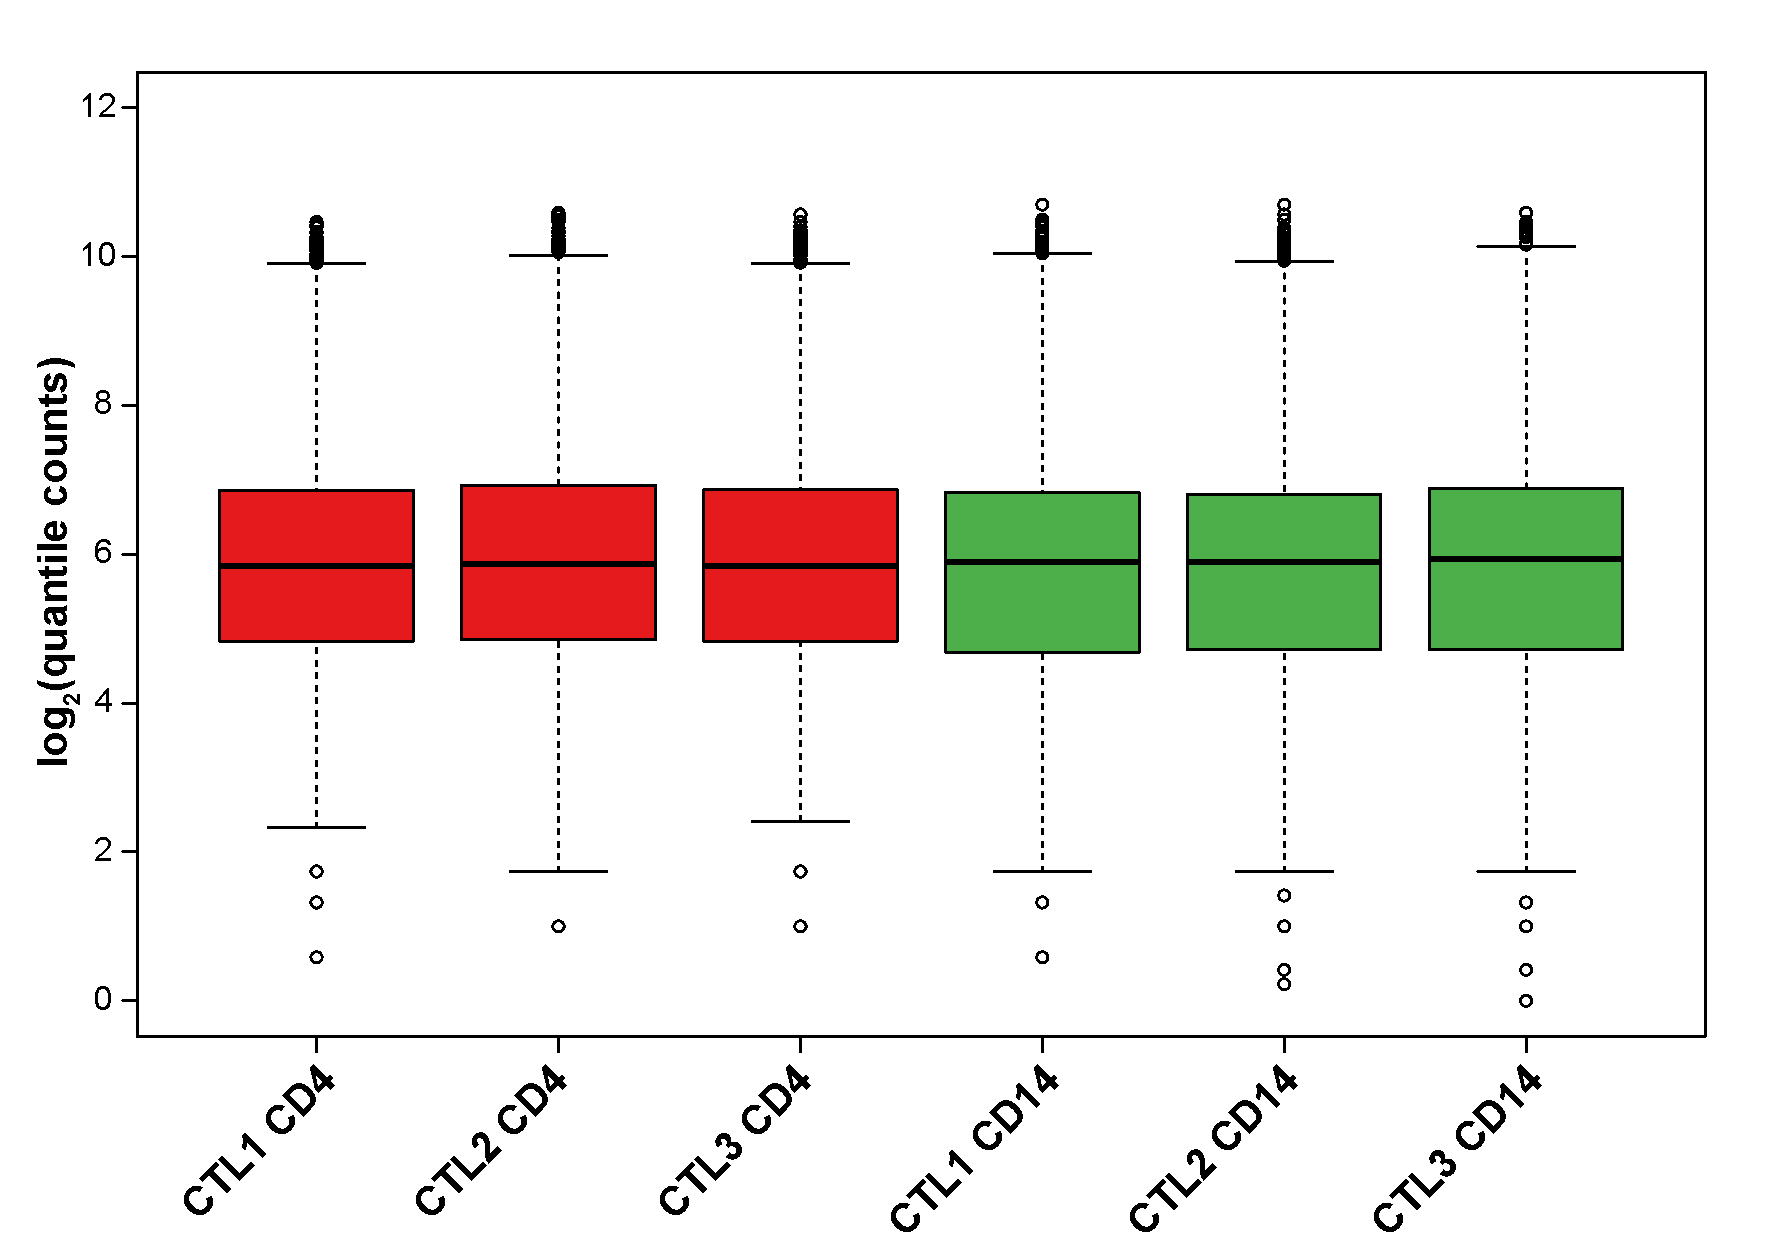
\includegraphics[width=\textwidth]{./Results1/pdfs/ATAC_Core_CD4_CD14_boxplot_80pcnt_cut_off_filtered_quantile_counts}
\caption{\textbf{}}
\end{subfigure}%
\begin{subfigure}{0.45\textwidth}
\centering
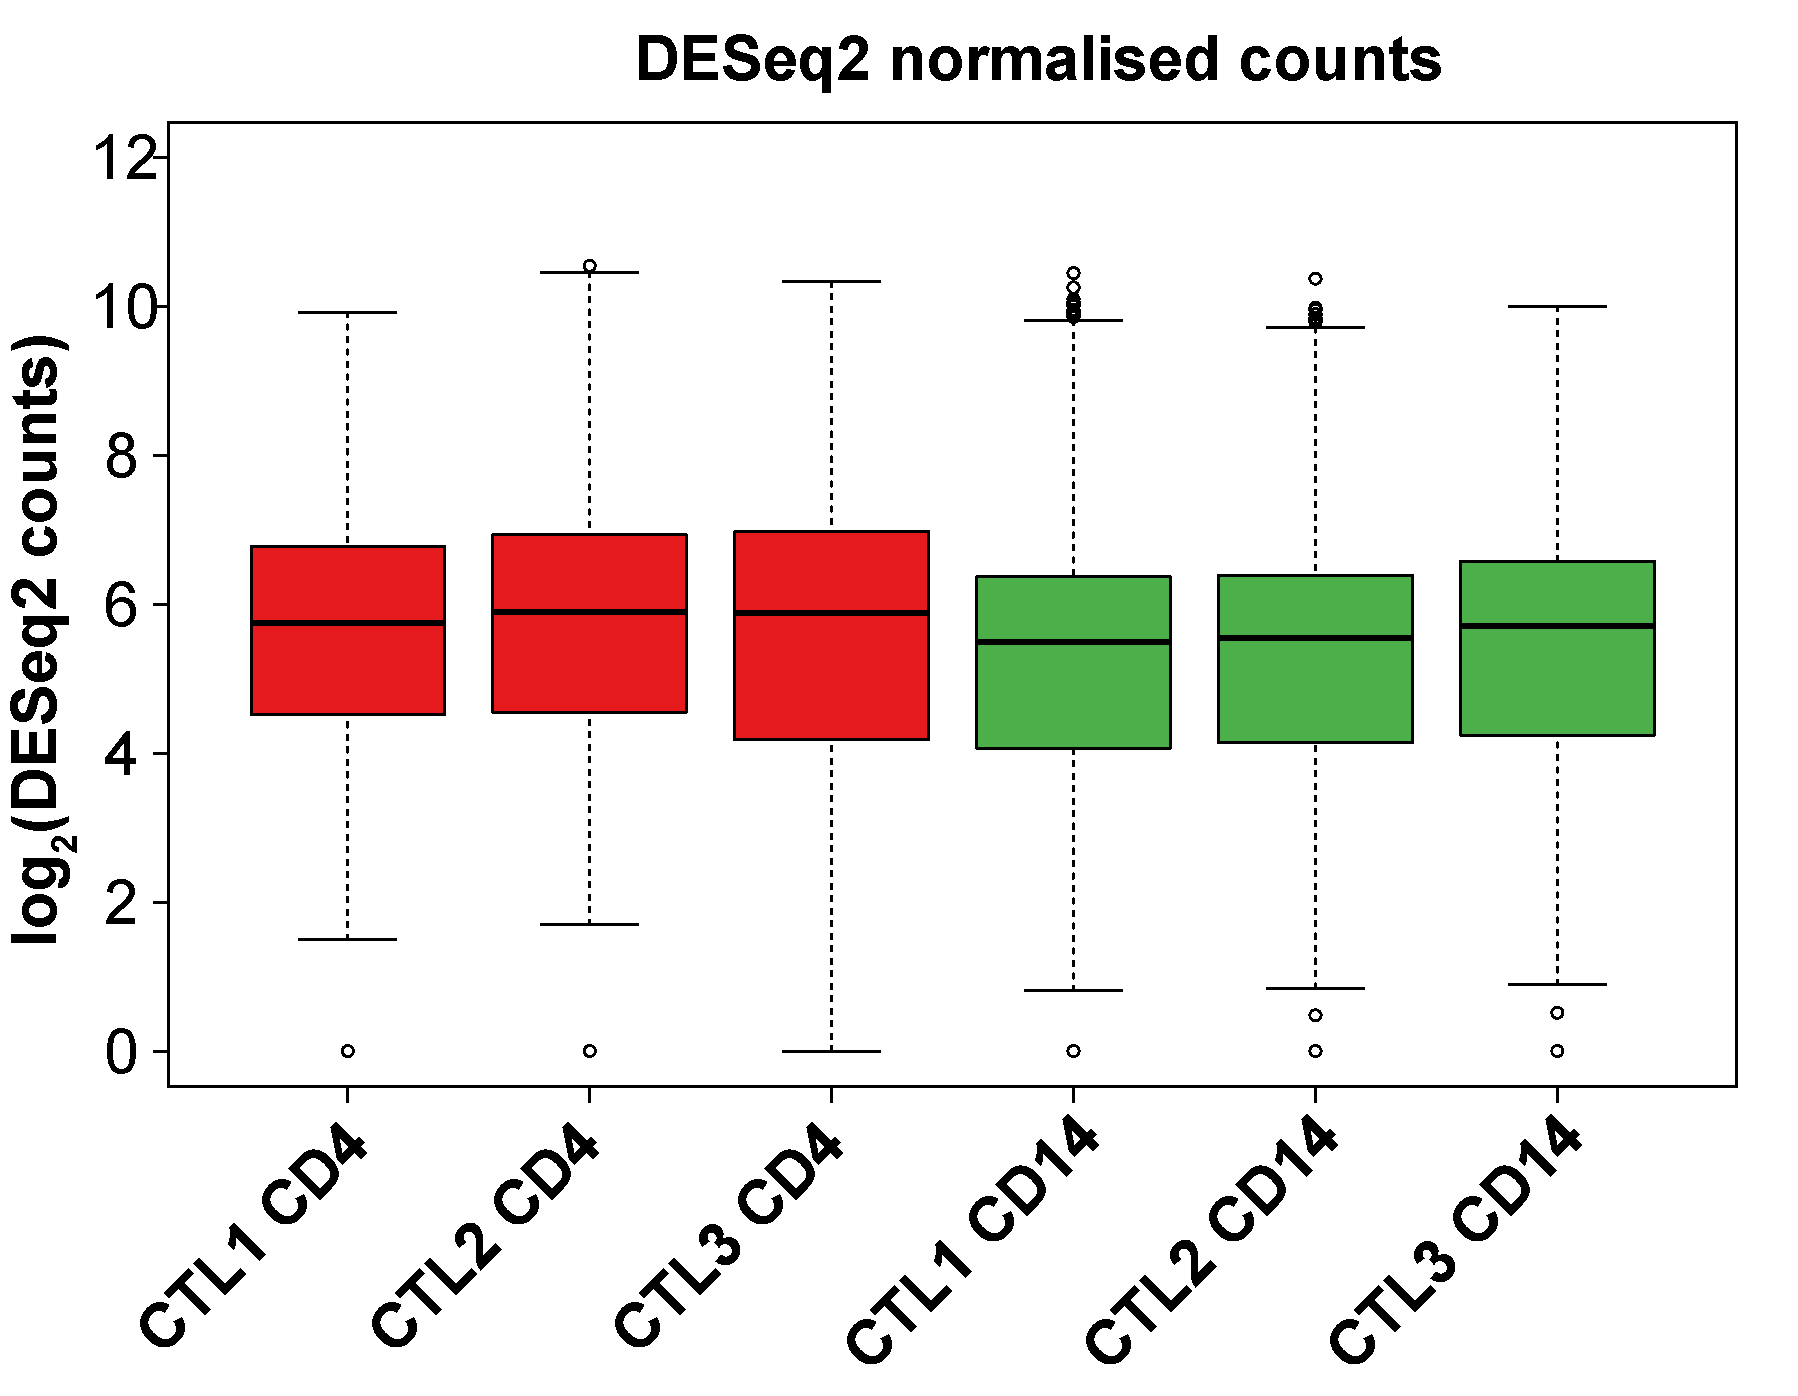
\includegraphics[width=\textwidth]{./Results1/pdfs/ATAC_Core_fastq_CD4_CD14_DESeq2_mean_vs_log2sd}
\caption{\textbf{}}
\end{subfigure}
\begin{subfigure}{0.5\textwidth}
\centering
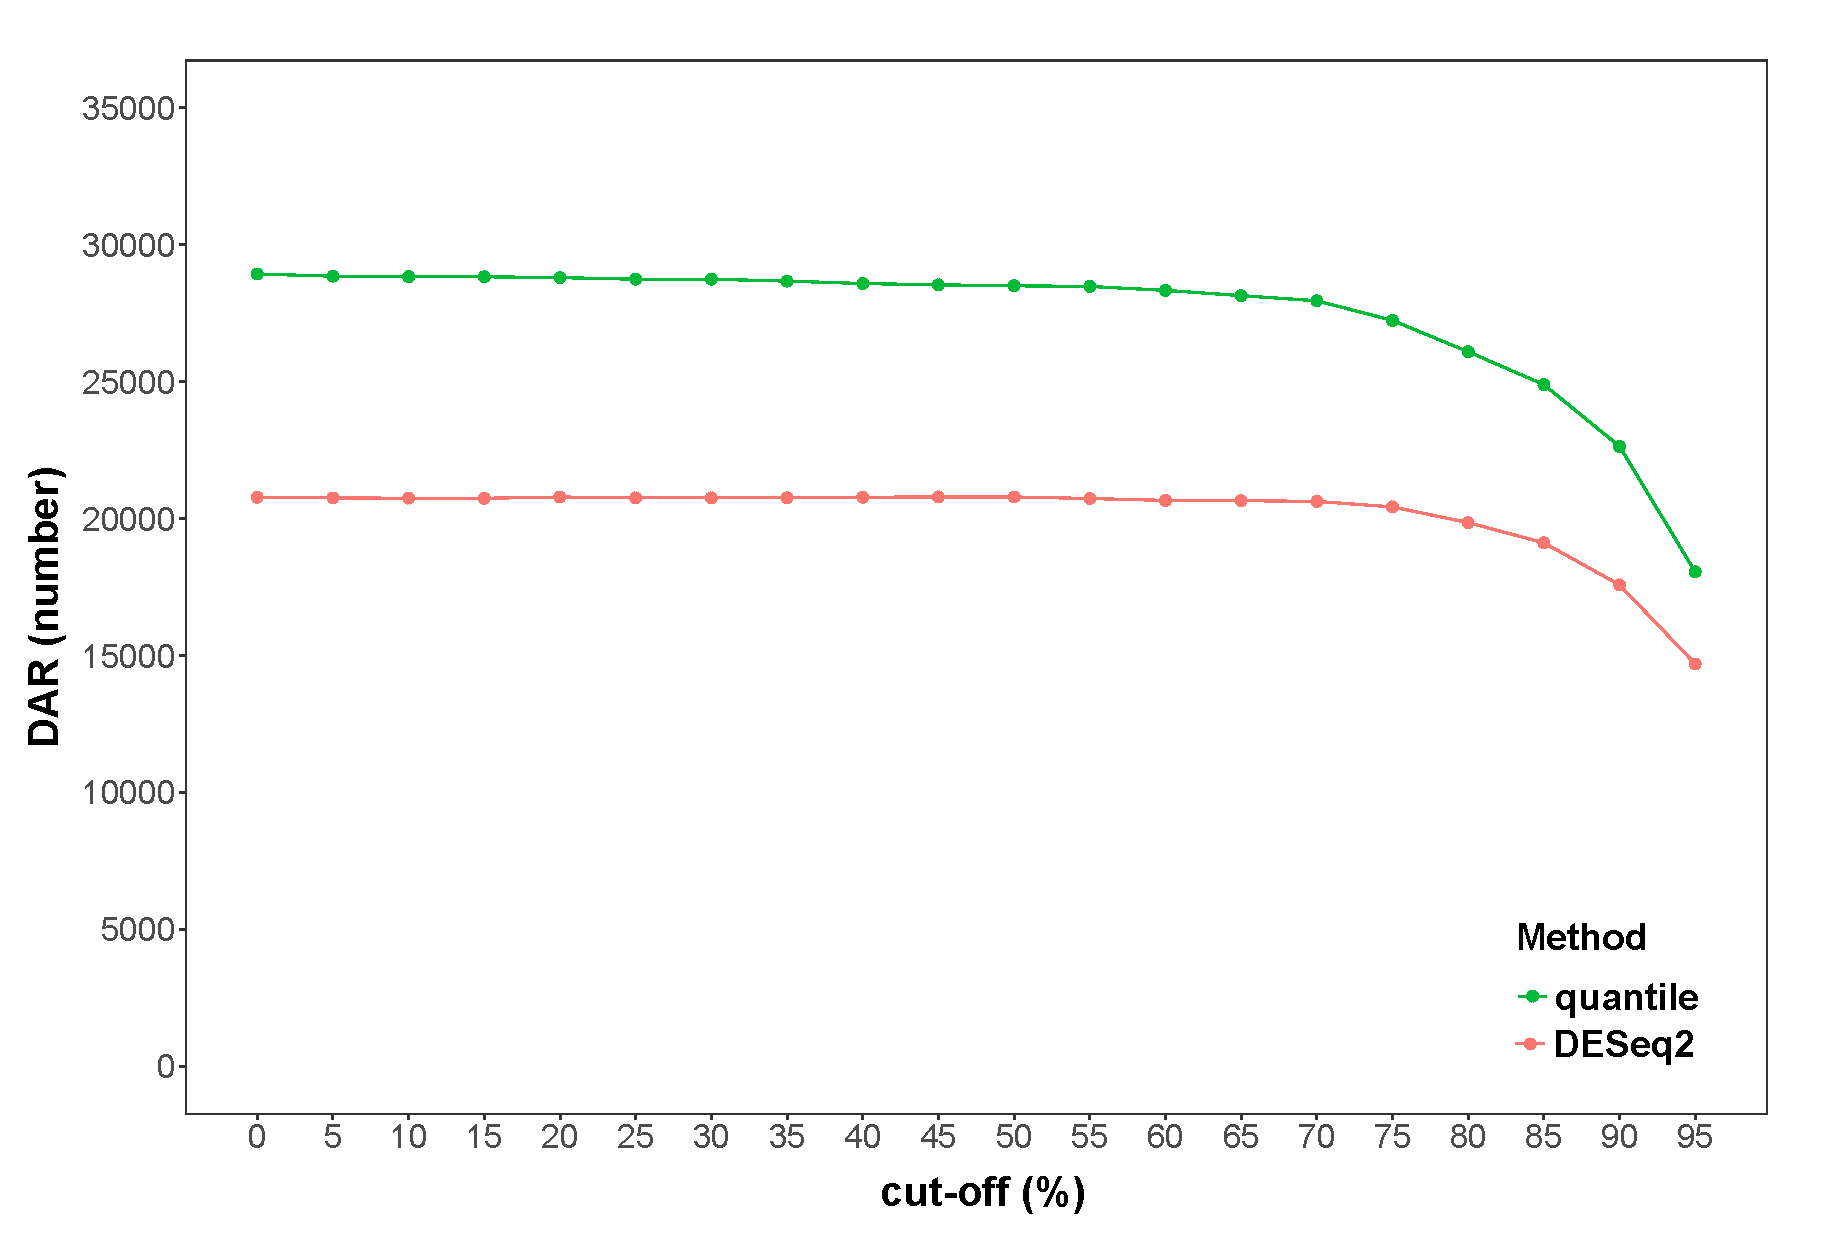
\includegraphics[width=\textwidth]{./Results1/pdfs/ATAC_Core_CD4vsCD14_DOC_FDR_01_vs_cutoffs_quantile_DESeq2_only}
\caption{\textbf{}}
\end{subfigure}

\caption[Normalisation and differential chromatin accessibility analysis for different cut-offs using quantile normalisation limma voom and DESeq2.]{\textbf{Normalisation and differential chromatin accessibility analysis for different cut-offs using quantile normalisation\& limma voom and DESeq2.} Boxplots representing the log$_2$  read counts for each of the peaks from the unfiltered consensus list of peaks normalised by (A) quantile or (B) DESeq2 in the three CD14$^+$ monocytes and total CD4$^+$  healthy control paired samples. (C) Representation of the number of significant DARs (FDR$<$0.01 and FC$>$1.5) detected in the differential analysis by limma voom (using quantile normalisation) or DESeq2 when using a sequence of empirical background noise cut-offs to filter the consensus list of peaks.}
\label{figure:ATAC_normalisation_and_DARs_limma_DESeq2}
\end{figure} 

This suggested a reduction in the number of false positive hits resulting from peaks with high background reads. However, increasingly stringent filtering would also remove true positives so an intermediate value of 80\% was chosen here. In future analyses this value may vary depending on the noise inherent to the experiment.



\begin{figure}[htbp]
\centering
\begin{subfigure}{0.5\textwidth}
\centering
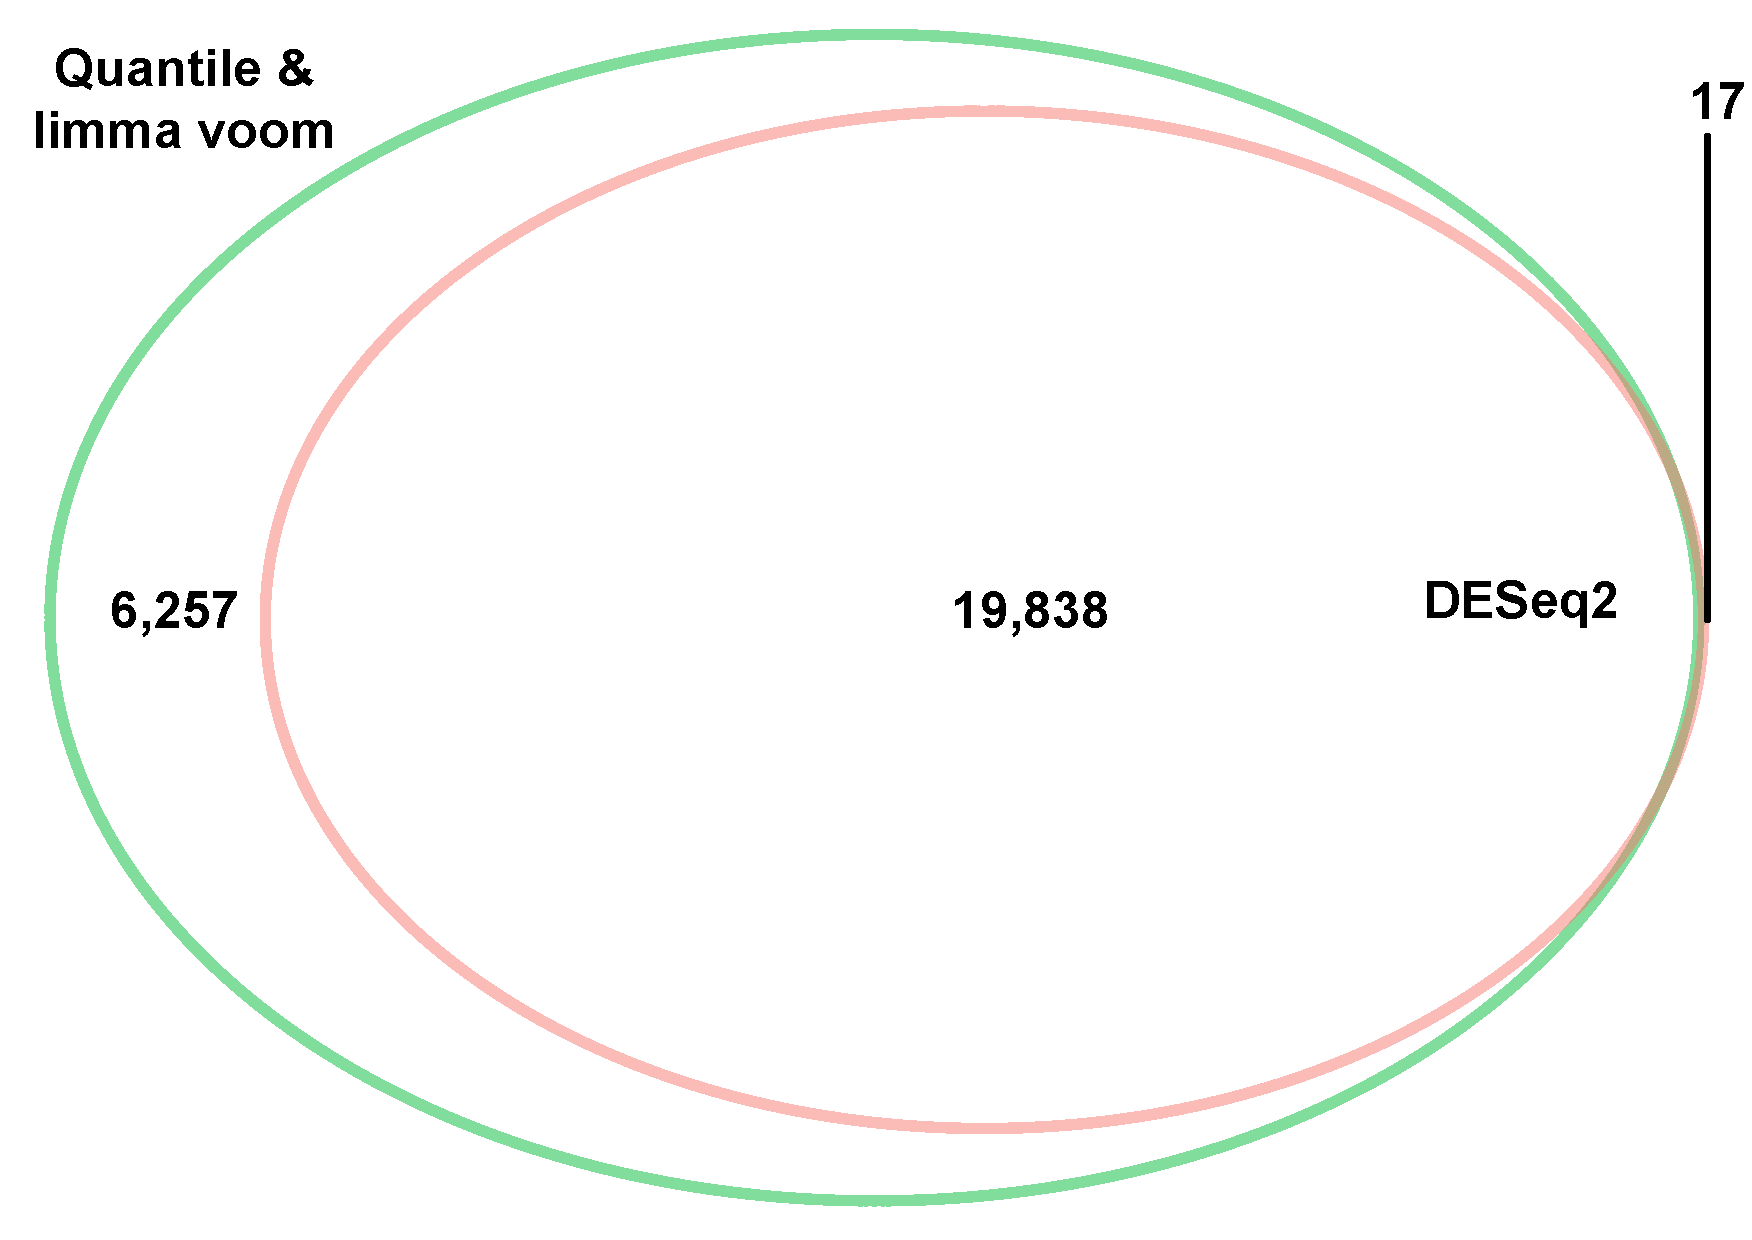
\includegraphics[width=\textwidth]{./Results1/pdfs/ATAC_Core_fresh_CD4vsCD14_venn_diagram_differential_analysis_FDR_01_quantile_DESeq2_only}
\caption{\textbf{}}
\end{subfigure}
\begin{subfigure}{0.5\textwidth}
\centering
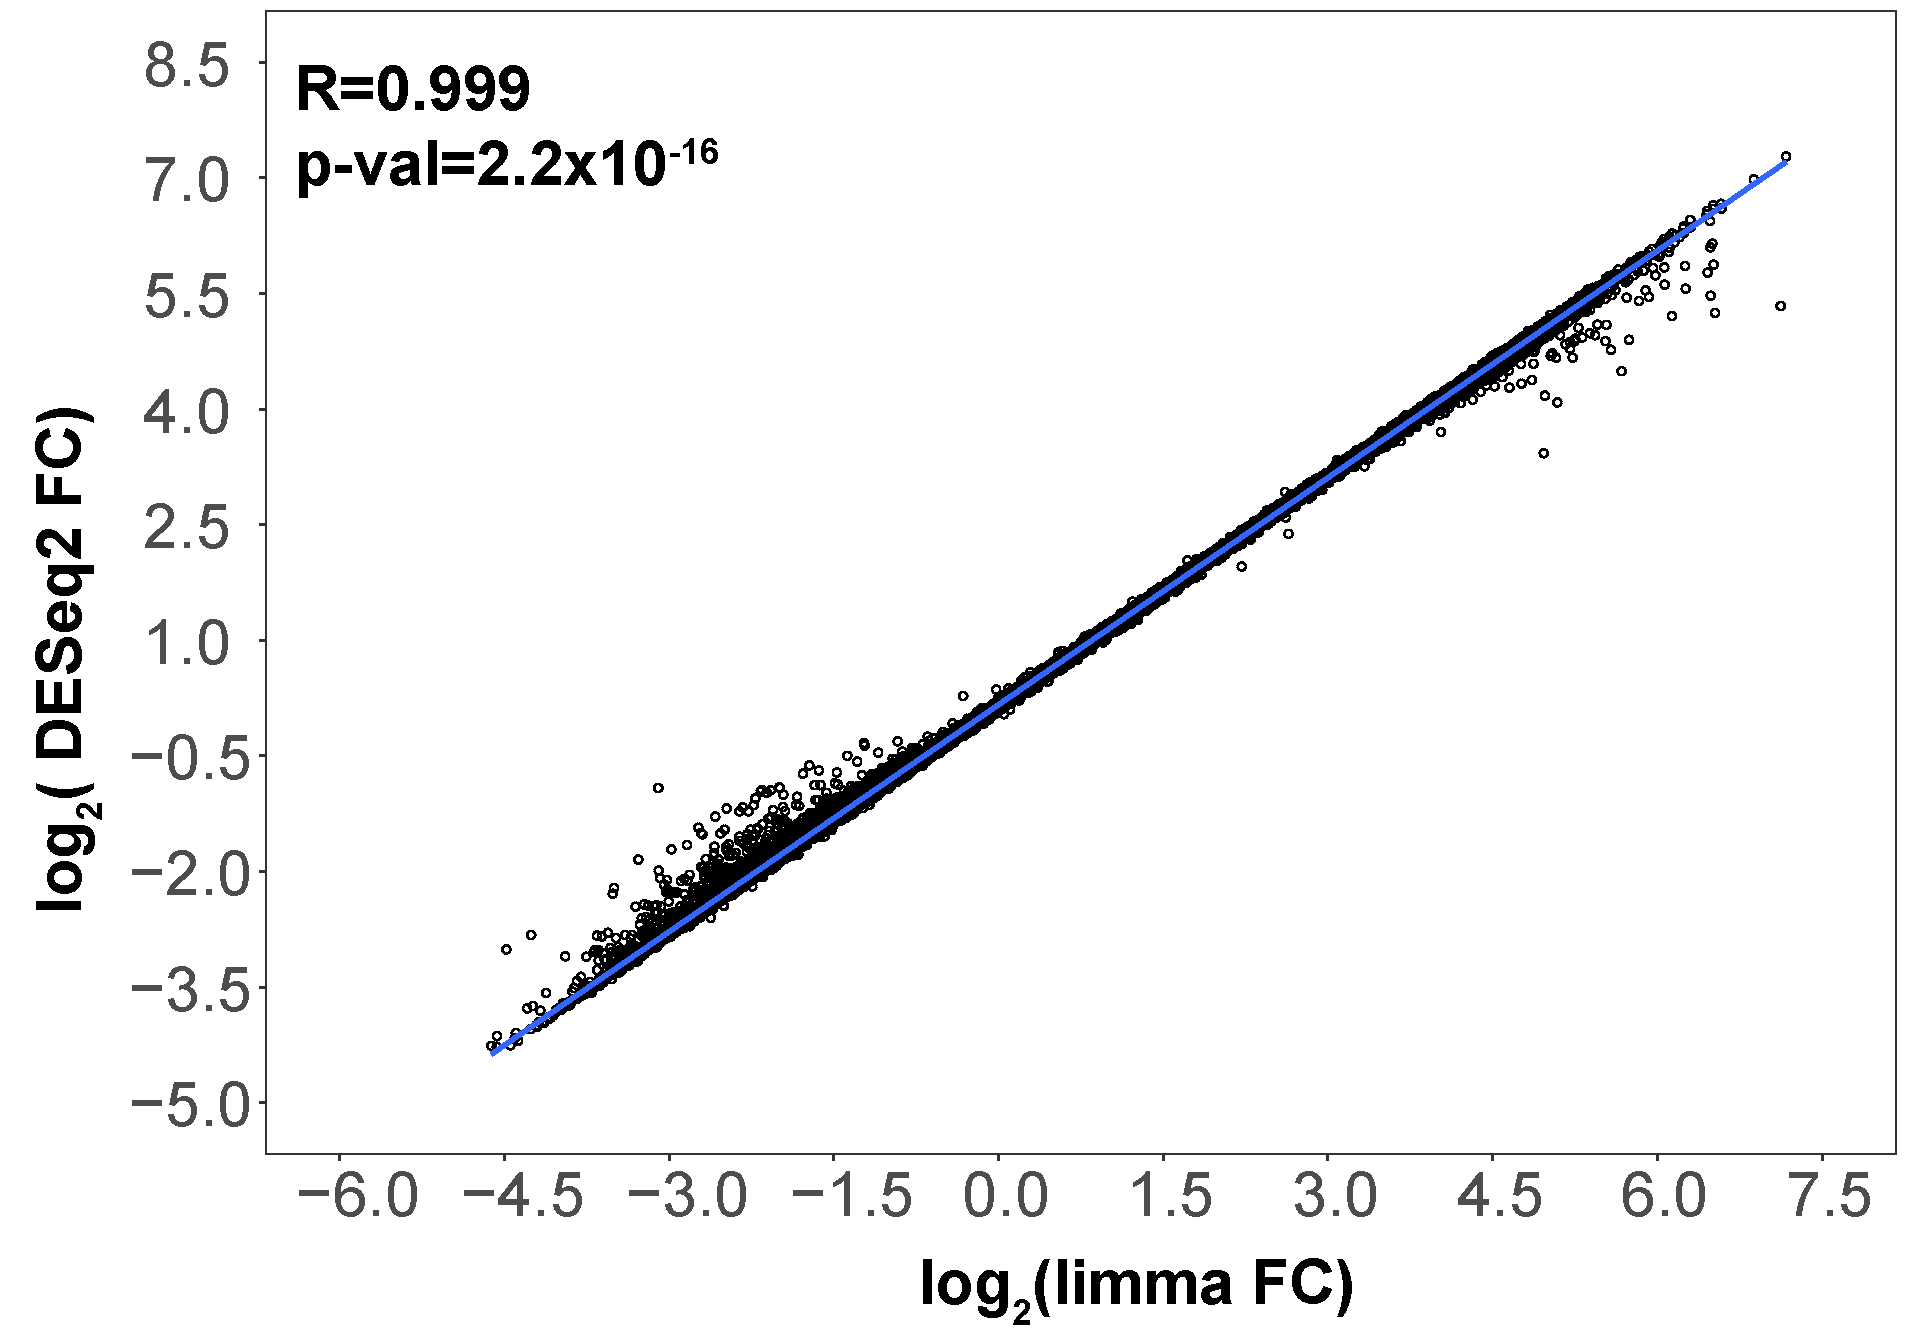
\includegraphics[width=\textwidth]{./Results1/pdfs/ATAC_Core_fastq_CD4_CD14_80pcnt_cut_off_correlation_log2FC_quantile_vs_deseq2}
\caption{\textbf{}} % to add text to the figure name
\end{subfigure}
\caption[Comparison of the DARs identified by differential analysis using limma voom or DESeq for the consensus peak list filtered at the optimal 80\% cut-off.]{\textbf{Comparison of the DARs identified by differential analysis using limma voom or DESeq for the consensus peak list filtered at the optimal 80\% cut-off.} (A) Venn diagram illustrating the common and distinct significant (FDR$<$0.01 and fold change$>$1.5) DARs identified by differential analysis in the filtered consenus list of ATAC peaksfor the 80\% optimal cut-off using limma voom or DESeq2. (B) Representation of the correlation between limma voom and DESeq2 log$_2$ fold changes (no FDR filtered) in each the peaks from the fconsensus list of peaks filtered at the 80\% optimal cut-off. Pearson correlation coefficient (R) and significance (p-value) are indicated. Limma voom was applied to quantile normalised count data.}
\label{figure:QC_quantile_DAR_and_DESeq2_comparison}
\end{figure} 


The vast majority of the 19,855  DARs called as significant using the more conservative method (DESeq2) were recapitulated by limma voom at the same significance threshold (FDR$<$0.01 and fold change$>$1.5) (Figure \ref{figure:QC_quantile_DAR_and_DESeq2_comparison}A). FDR rank revealed that out of the first 19,855 limma voom DARs 18,768 matched the rank of those retrieved by DESeq2. Moreover, very significant positive correlation was found between fold changes for all the regions included in the 80\% cut-off reduced matrix reported by the two methods (R=0.999, p-value=2.2$^{-16}$) (Figure \ref{figure:QC_quantile_DAR_and_DESeq2_comparison}B). Overall, this suggested that the differences in the number of significant DARs reported by limma voom and DESeq2 could partly be driven by differences in the models used by the two methods to estimate dispersion of counts. 

Lastly, the significant  DARs identified by DESeq2 and filtered for FDR$<$0.01 and fold change$>$1.5 were divided in those more accessible in CD14$^+$ monocytes  (open in monocytes) or CD4$^+$ (open in CD4$^+$). Enrichment analysis for cell type-specific epigenetic features, including FANTOM5 eRNAs, histone marks and DHSs, was conducted in each of the two groups of DARs. The CD4$^+$ open DARs were enriched for T cell eRNAs, CD4$^+$ H3Kme1 and H3K27ac and CD14$^+$ DHSs (Figure \ref{figure:Enrichment_analysis_of_DARs_by_DESeq2}). Conversely, the top enriched features for CD14$^+$ monocytes open DARs included eRNAs, H3K27ac and DHSs in monocytes. Overall, this enrichment analysis confirmed the ability of this differential analysis method to identify significant and robust DARs that highlight cell-type specific regulatory regions for CD14$^+$ monocytes and CD4$^+$ cells.

\begin{figure}[h]
\centering
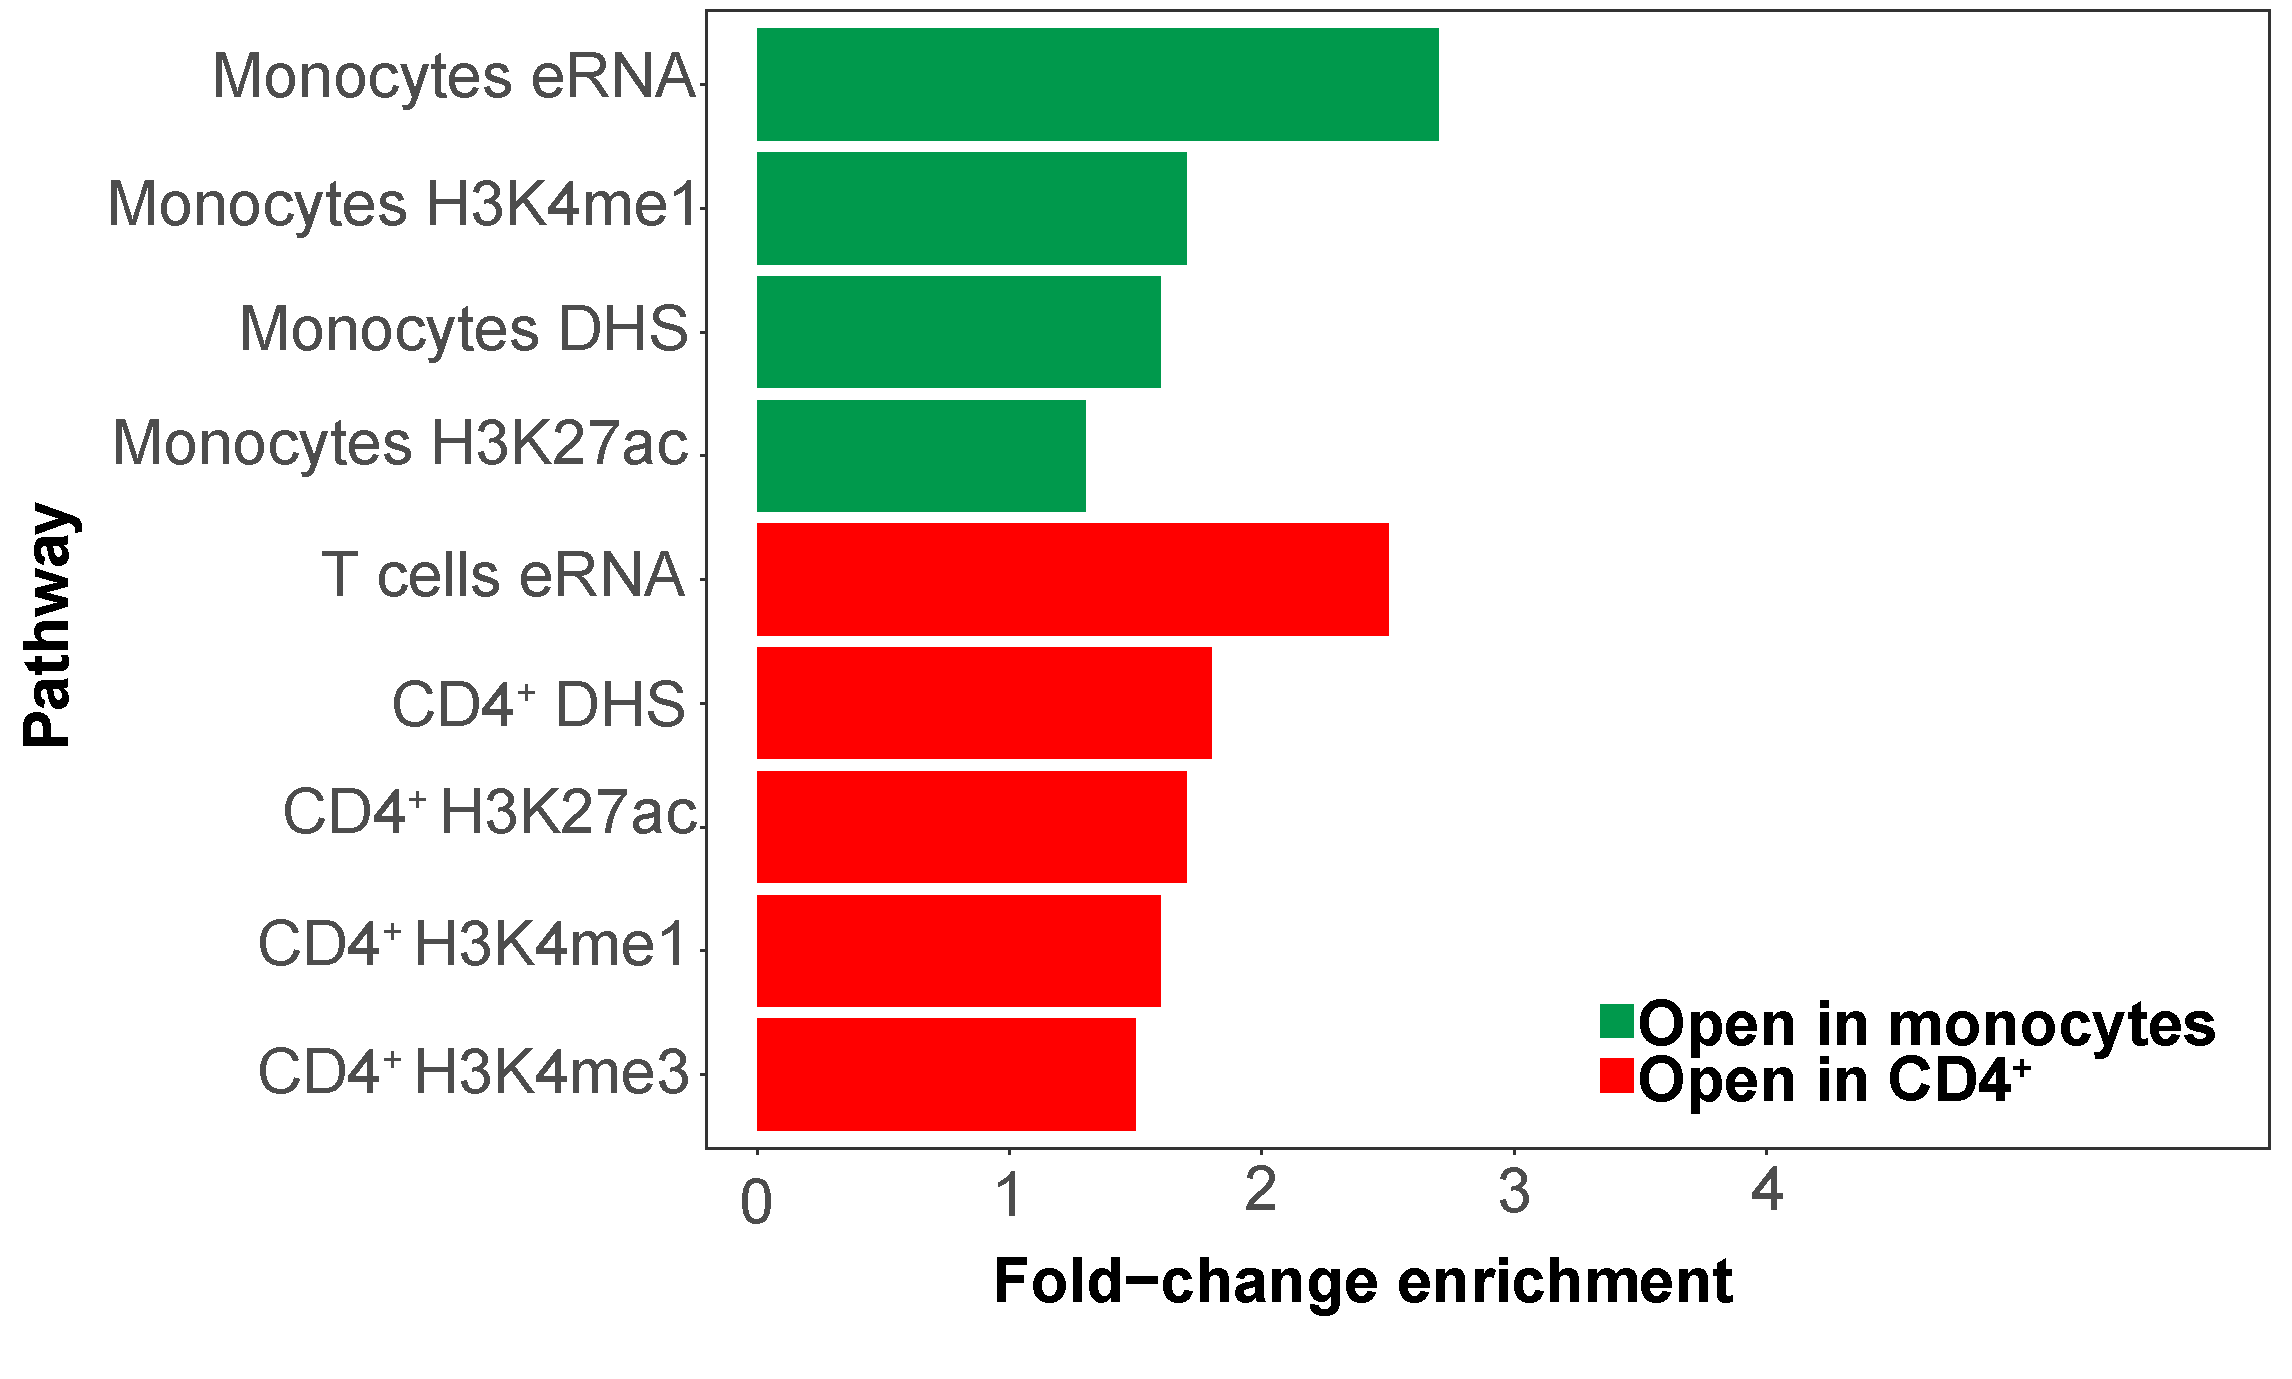
\includegraphics[width=0.6\textwidth]{./Results1/pdfs/ATAC_CD4vsCD14_deseq_features_enrichment_barplot}
\caption[Enrichment analysis for the significant DARs identified by DESeq2 between CD14$^+$ monocytes and CD4$^+$ cells.]{\textbf{Enrichment analysis for the significant DARs identified by DESeq2 between CD14$^+$ monocytes and CD4$^+$ cells.} Barplot representing the fold change for the top significantly enriched (FDR$<$0.01) FANTOM5 eRNAs, histone marks and DHSs from Blueprint. Enrichment analysis was performed separately for the significant (FDR$<$0.01 and fold change$>$1.5) DARs more accessible in CD14$^+$ monocytes (open in monocytes) or CD4$^+$ (open in CD4$^+$).}
\label{figure:Enrichment_analysis_of_DARs_by_DESeq2}
\end{figure} 



%\begin{figure}[htbp]
%\centering
%\begin{subfigure}{0.65\textwidth}
%\centering
%\includegraphics[width=\textwidth]{./Results1/pdfs/ATAC_Core_CD4vsCD14_clusters_and_heatmap_DESeq2_only}
%\caption{\textbf{}}
%\end{subfigure}
%\begin{subfigure}{0.5\textwidth}
%\centering
%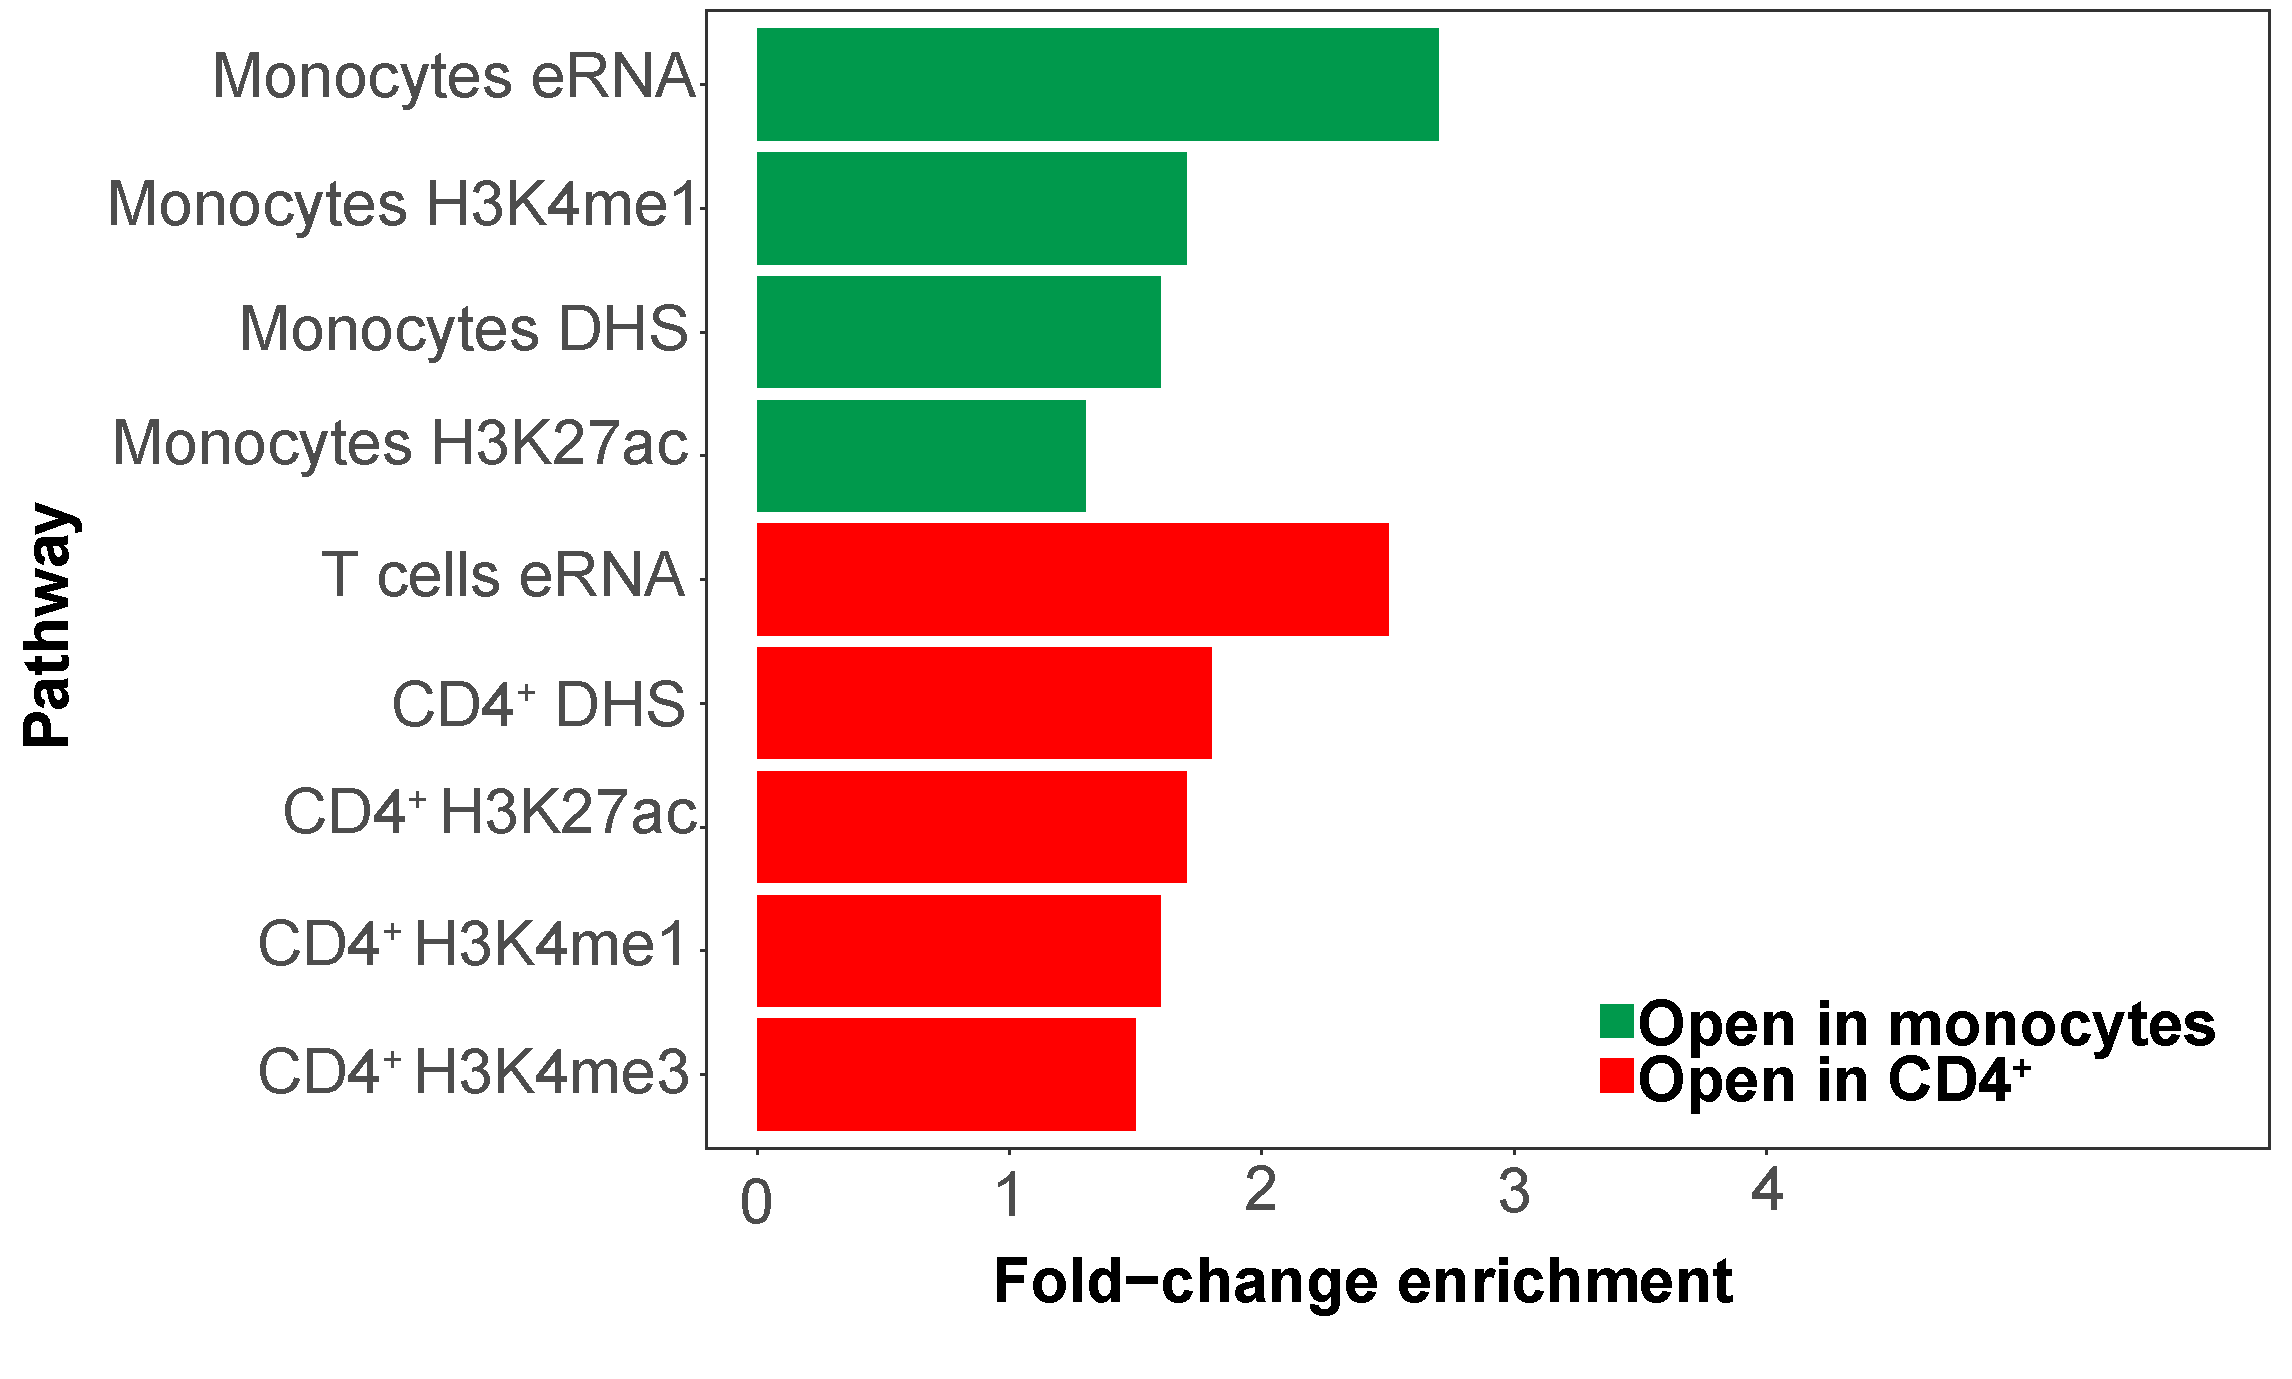
\includegraphics[width=\textwidth]{./Results1/pdfs/ATAC_CD4vsCD14_deseq_features_enrichment_barplot}
%\caption{\textbf{}} % to add text to the figure name
%\end{subfigure}
%\caption[Clustering heatmap and enrichment analysis for the significant DARs identified by DESeq2 between CD14$^+$ monocytes and CD4$^+$ cells.]{\textbf{Clustering heatmap and enrichment analysis for the identified DARs by DESeq2 between CD14$^+$ monocytes and CD4$^+$ cells.} (A)Heatmap showing for each of the ATAC-seq samples included in this analysis, the log$_2$ normalised counts at each of the 19,838 significant (FDR$<$0.01 and abs(fold change)$>$1.5) DARs identified by DESeq2. Each row represents a DAR and are clustered based on DARs presenting similar patterns of accessibility in each of the three replicates for the two cell types compared. (B) Barplot representing the fold change for the top significantly enriched (FDR$<$0.01) FANTOM5 eRNAs and Blueprint histone marks and DHSs.}
%\label{figure:Heatmap_and_enrichment_analysis_of_DARs_by_DESeq2}
%\end{figure} 
%

\bigskip %bigger space



\subsection{Assessment of ATAC-seq transposition times in relevant cell types}
\label{ATACseq}

The duration of the transposition reaction was further investigated for the main immune cell types of interest for this thesis. ATAC-seq was performed for three different transposition times (20, 30 and 40 min) in CD14$^+$ monocytes, CD4$^+$, total CD8$^+$ (CD8$^+$) and CD19$^+$ cells in one healthy control sample included in cohort 1A from Chapter \ref{ch:Results2} (Tables \ref{tab:Summary_all_cohorts} and \ref{tab:Control_cohort_metadata}). The impact of transposition times in a number of ATAC related readouts was explored. The duration of the transposition, the concentration of Tn5 and the number of cells can have an effect on the relative proportion of nucleosome-free vs nucleosome-bound (mono-nucleosomes and beyond) regions tagged by the adapters. Ideally, the transposition reaction should yield NFF ($\leq$150bp), where TF and other proteins bind, without losing mono- and di-nucleosome fragments characteristic of the ATAC libraries. In this case, all three transposition times produced appropriate fragment size distributions which recapitulated the ATAC characteristic nucleosome periodicity pattern (Figure \ref{figure:Transposition_times_ATAC}A). This was reflected by the ratio of NFF vs mono-nucleosome bound fragments (mNBF) (151-250bp, the most abundant of the nucleosome-bound fraction) being around 1, which indicates at least similar abundance of both types of fragments. The variation of this ratio with the transposition times showed very moderate changes and was heterogenous across cell types (Figure \ref{figure:Transposition_times_ATAC}B). For example, CD8$^+$ presented the greatest NFF/mNBF ratio for 20 min of transposition whereas the NFF/mNBF ratio reached a maximum at 40 min for the CD14$^+$ monocytes. Overall, the tested transposition times in this experiment showed neglectable impact on the NFF/mNBF ratio, which was lower than 7 (cut-off to designate ATAC libraries lacking appropriate fragment size distribution according to Alasoo and colleagues \parencite{Alasoo2018}) in all instances. 

\begin{figure}[ht]
\centering
\begin{subfigure}{0.5\textwidth}
\centering
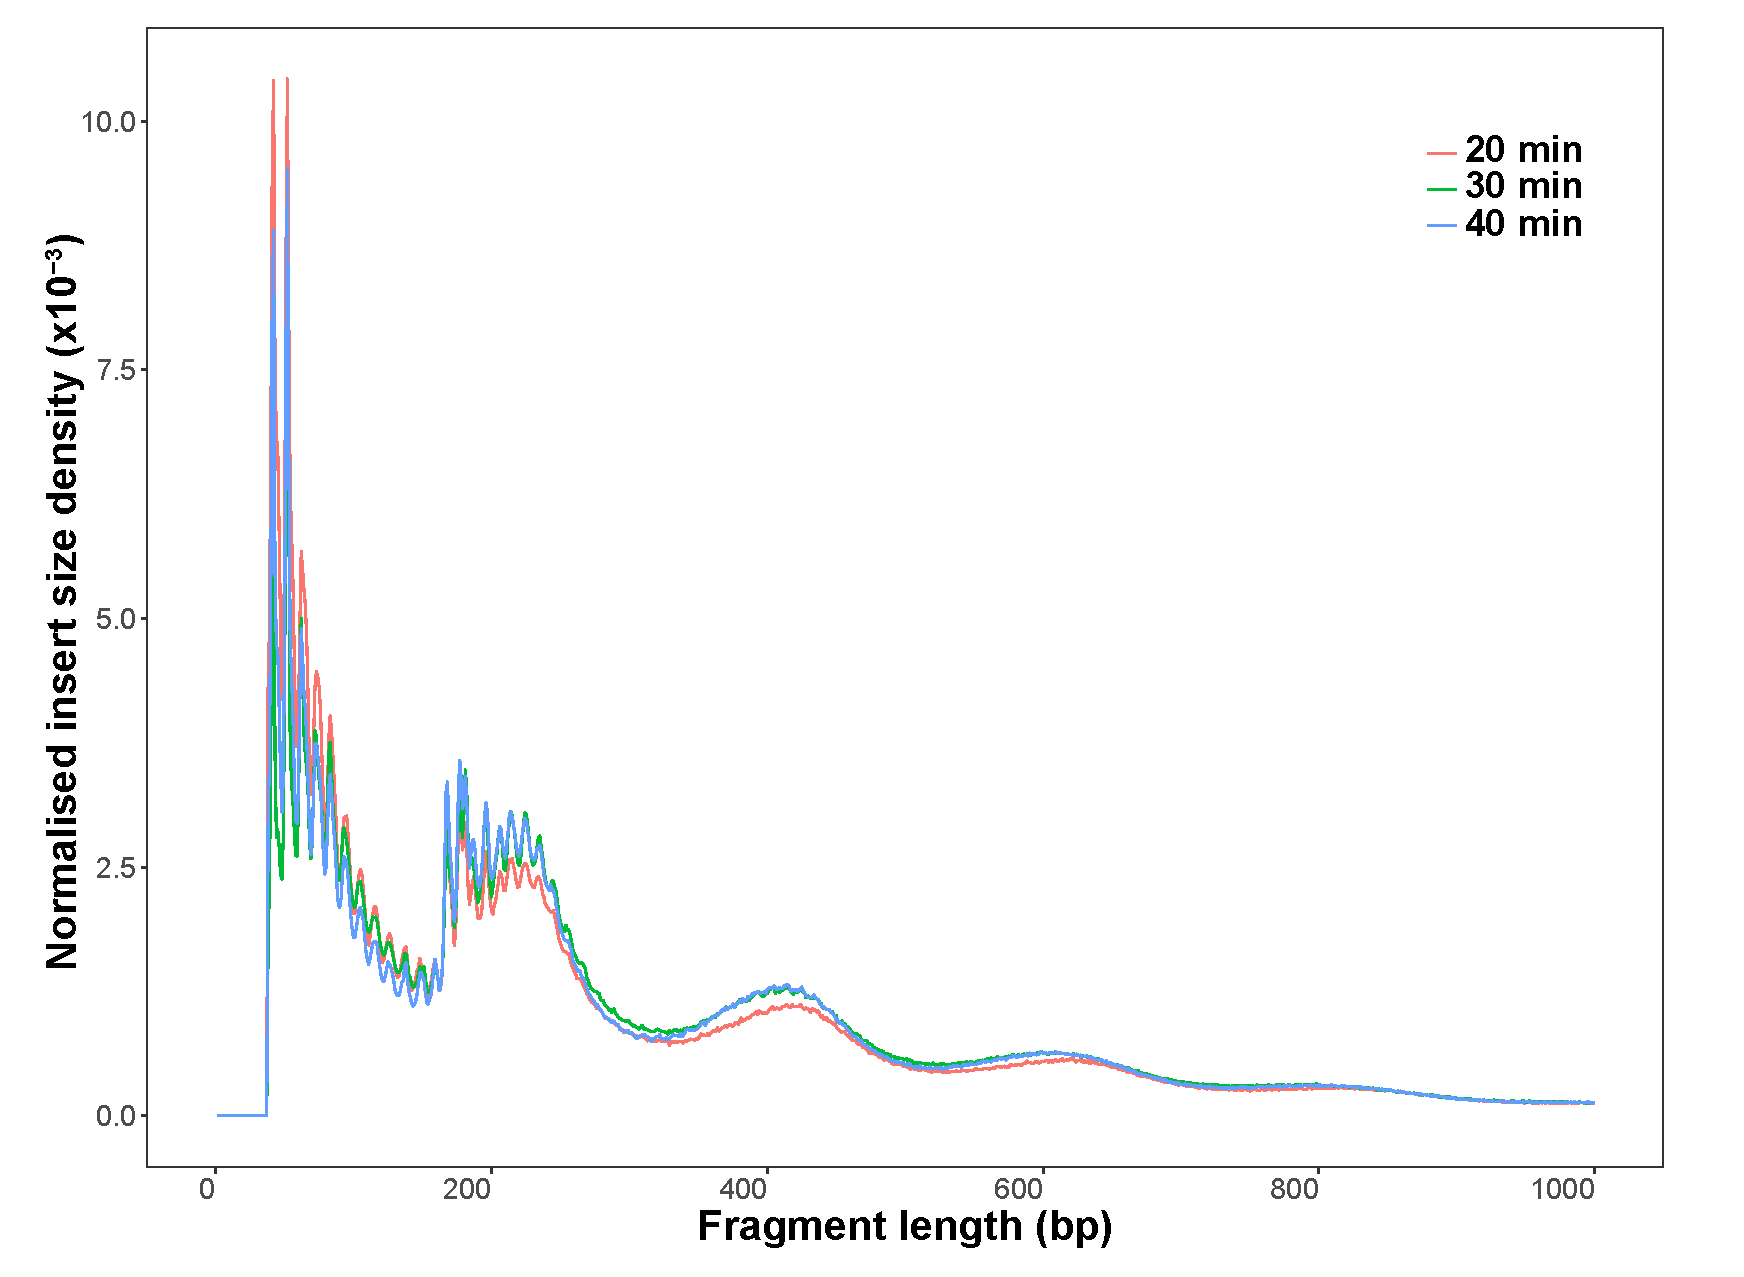
\includegraphics[width=\textwidth]{./Results1/pdfs/ATAC_CD8_fragment_size_distribution_20_30_40min}
\caption{\textbf{}}
% The percentage sign indicated that the other subfig goes side by side
\end{subfigure}%
\begin{subfigure}{0.5\textwidth}
\centering
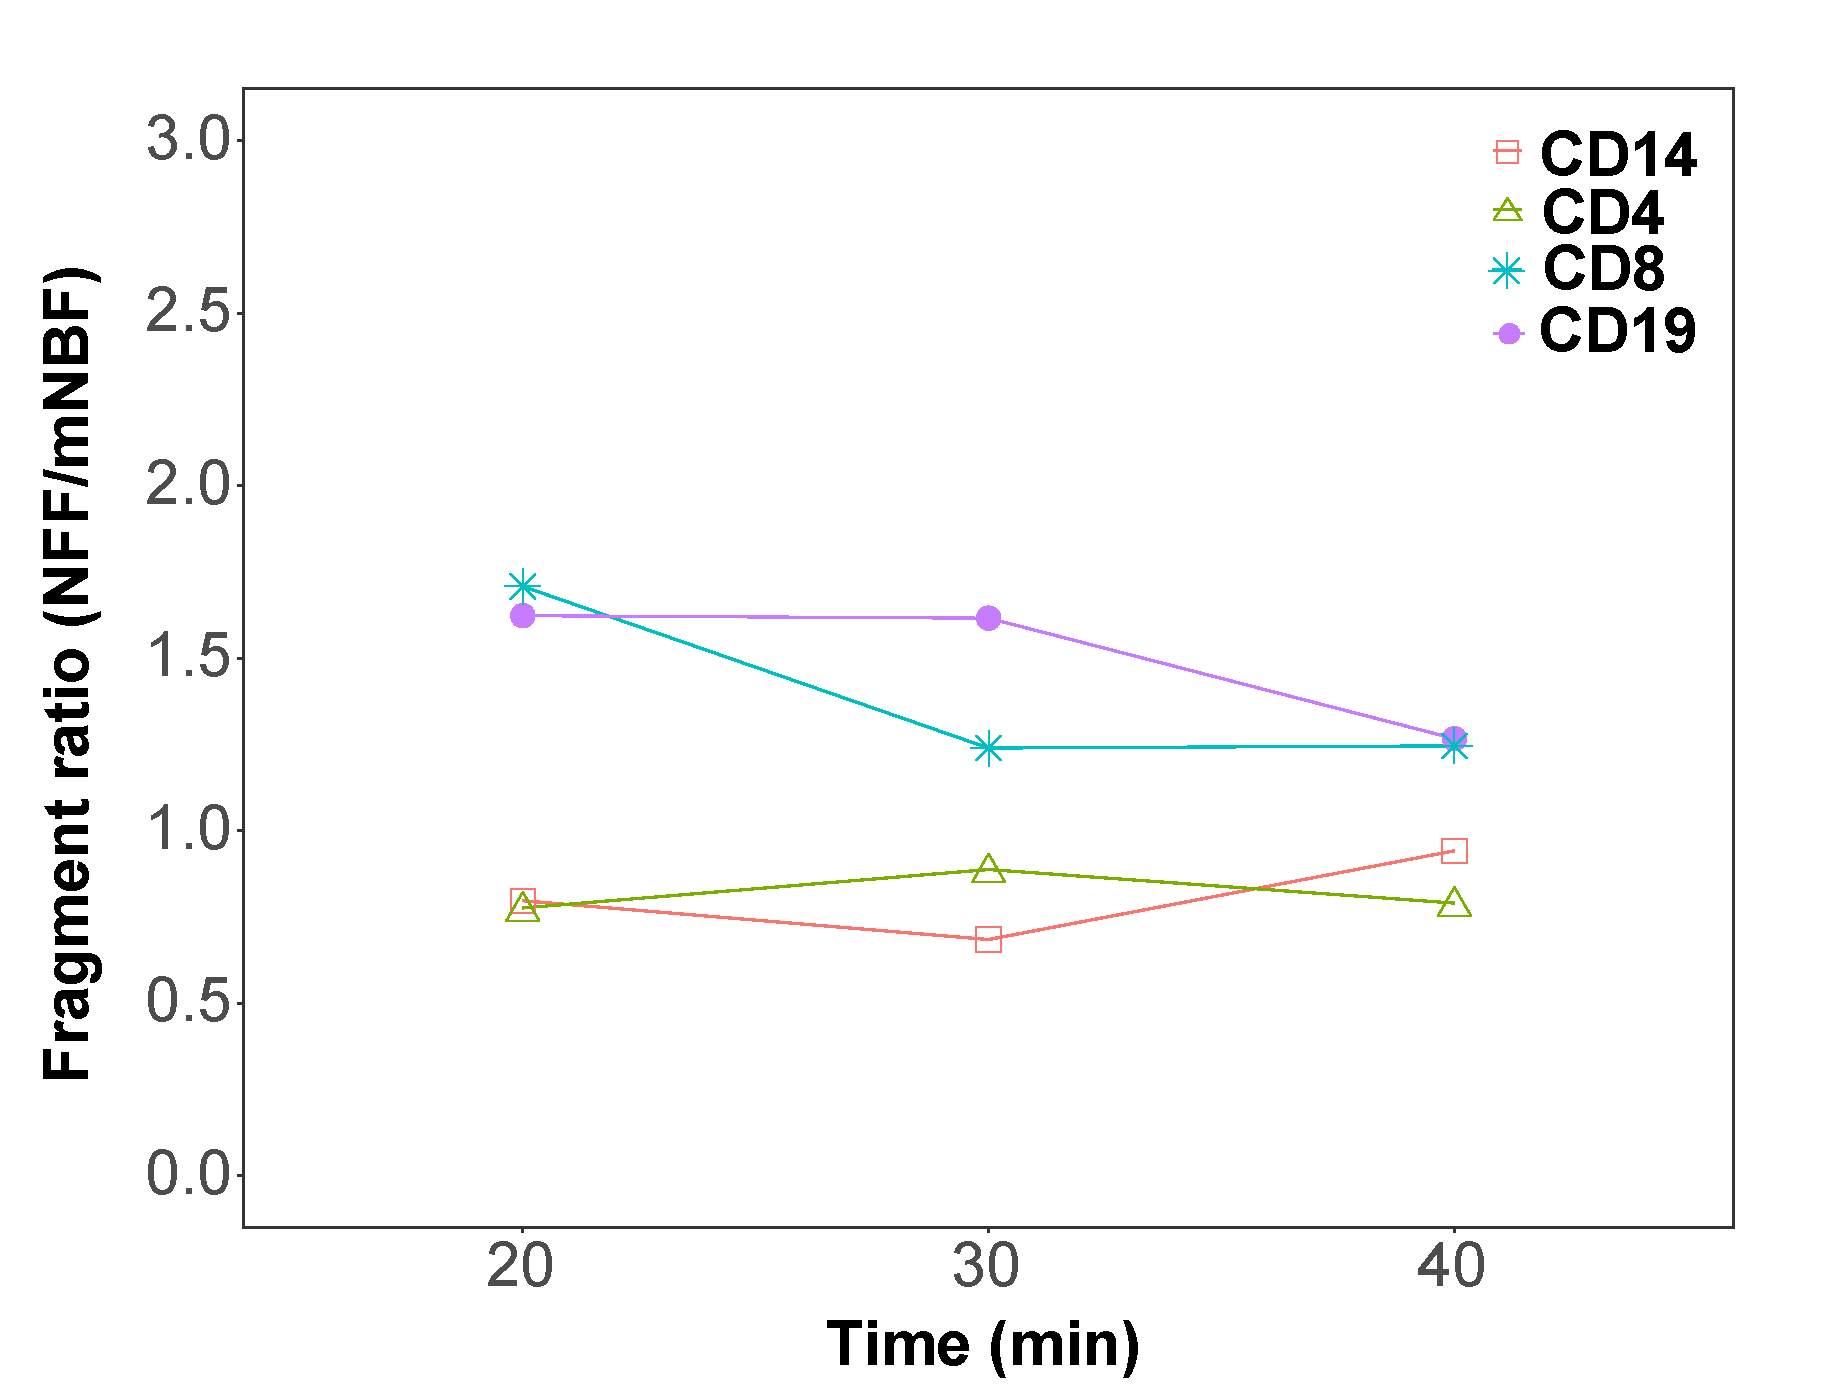
\includegraphics[width=\textwidth]{./Results1/pdfs/ATAC_ratio_short_long_fragments_mononucleosomes_20_30_40_min}
\caption{\textbf{}}
\end{subfigure} \\
\begin{subfigure}{0.5\textwidth}
\centering
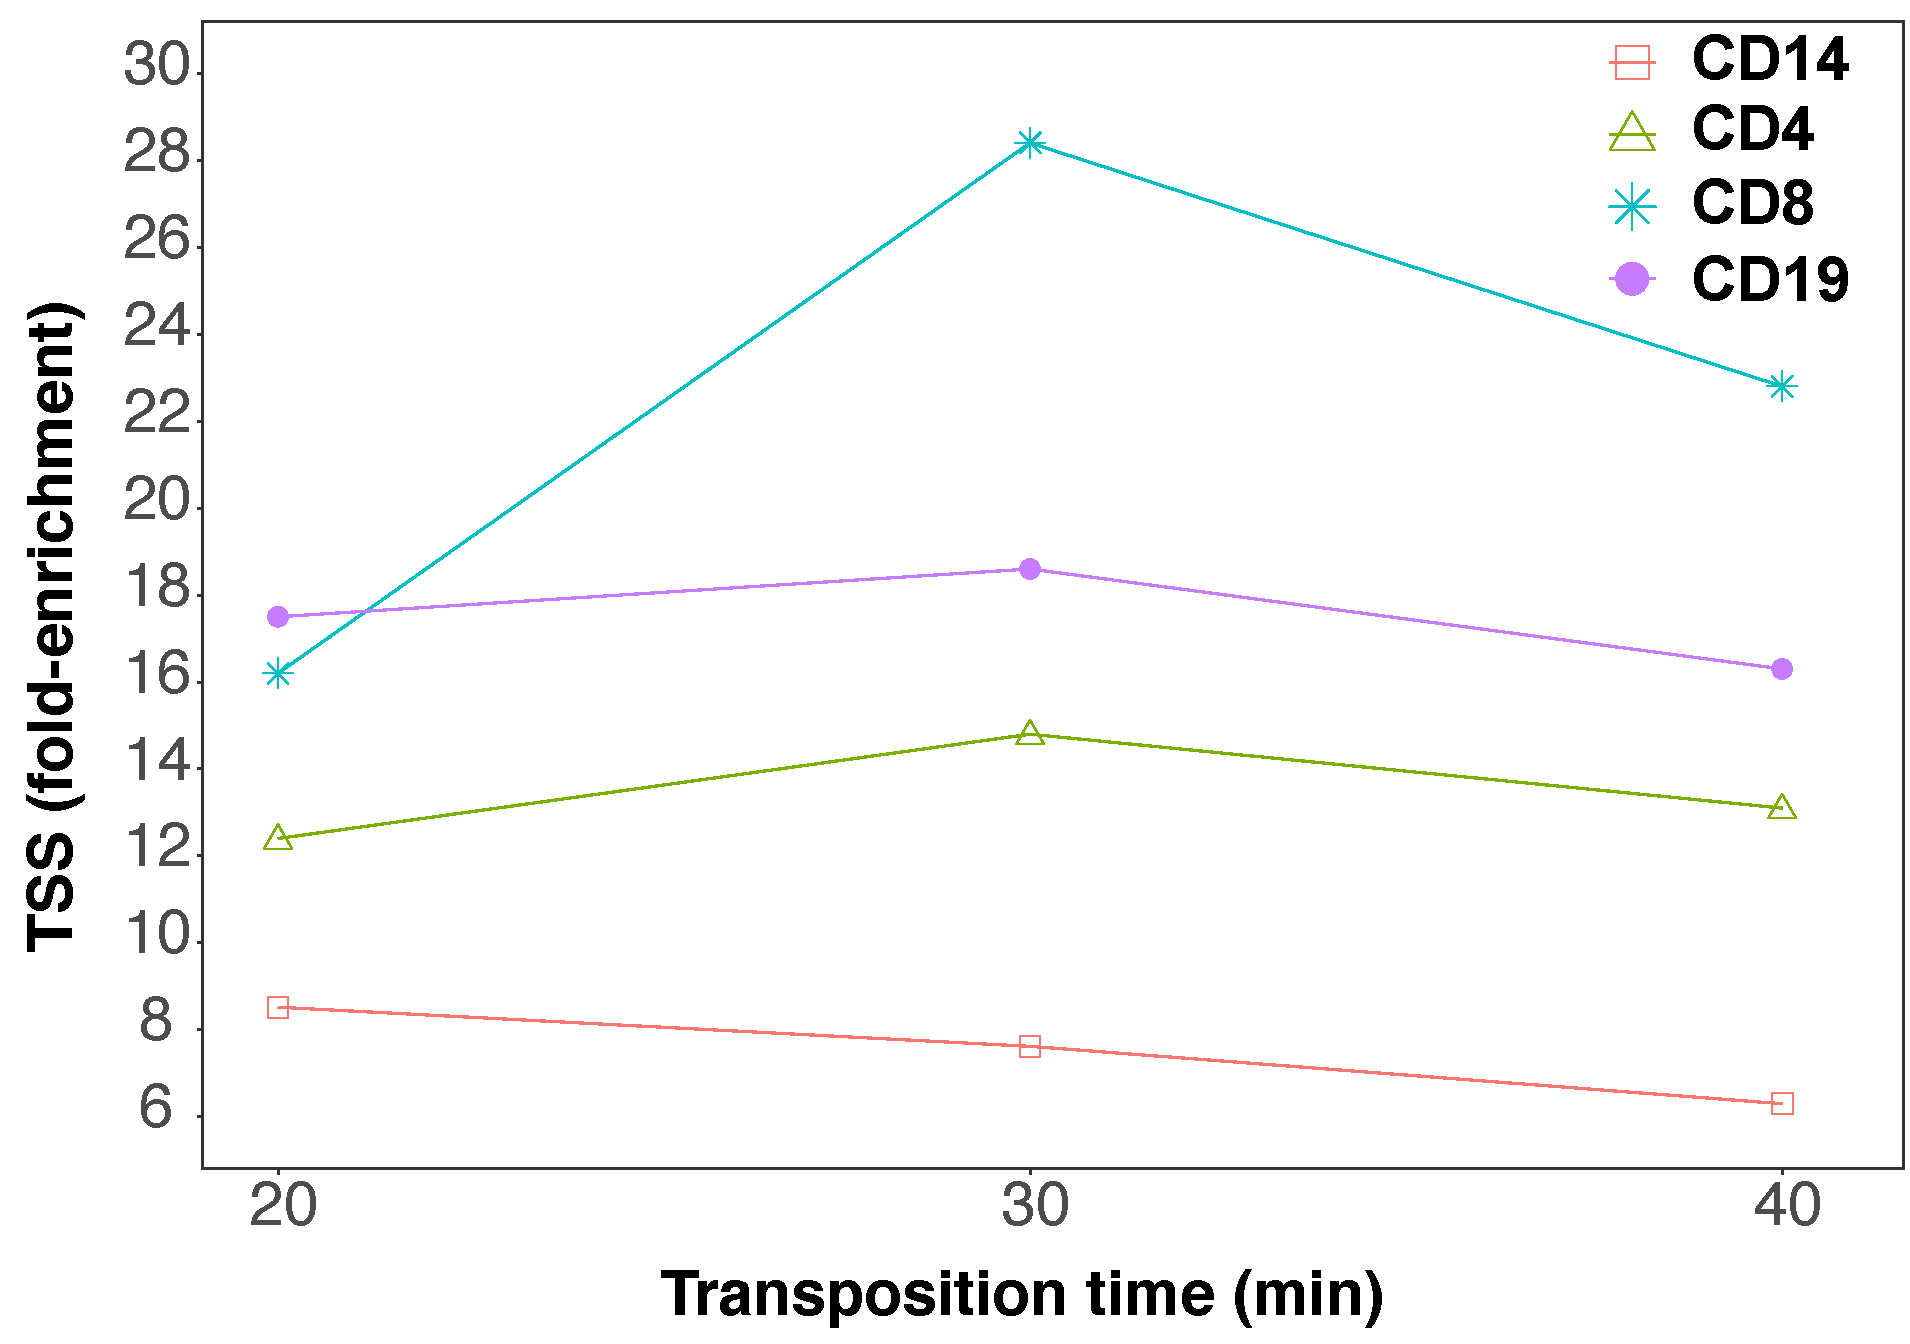
\includegraphics[width=\textwidth]{./Results1/pdfs/ATAC_TSS_vs_transposition_times}
\caption{\textbf{}} % to add text to the figure name
\end{subfigure}%
\begin{subfigure}{0.5\textwidth}
	\centering
	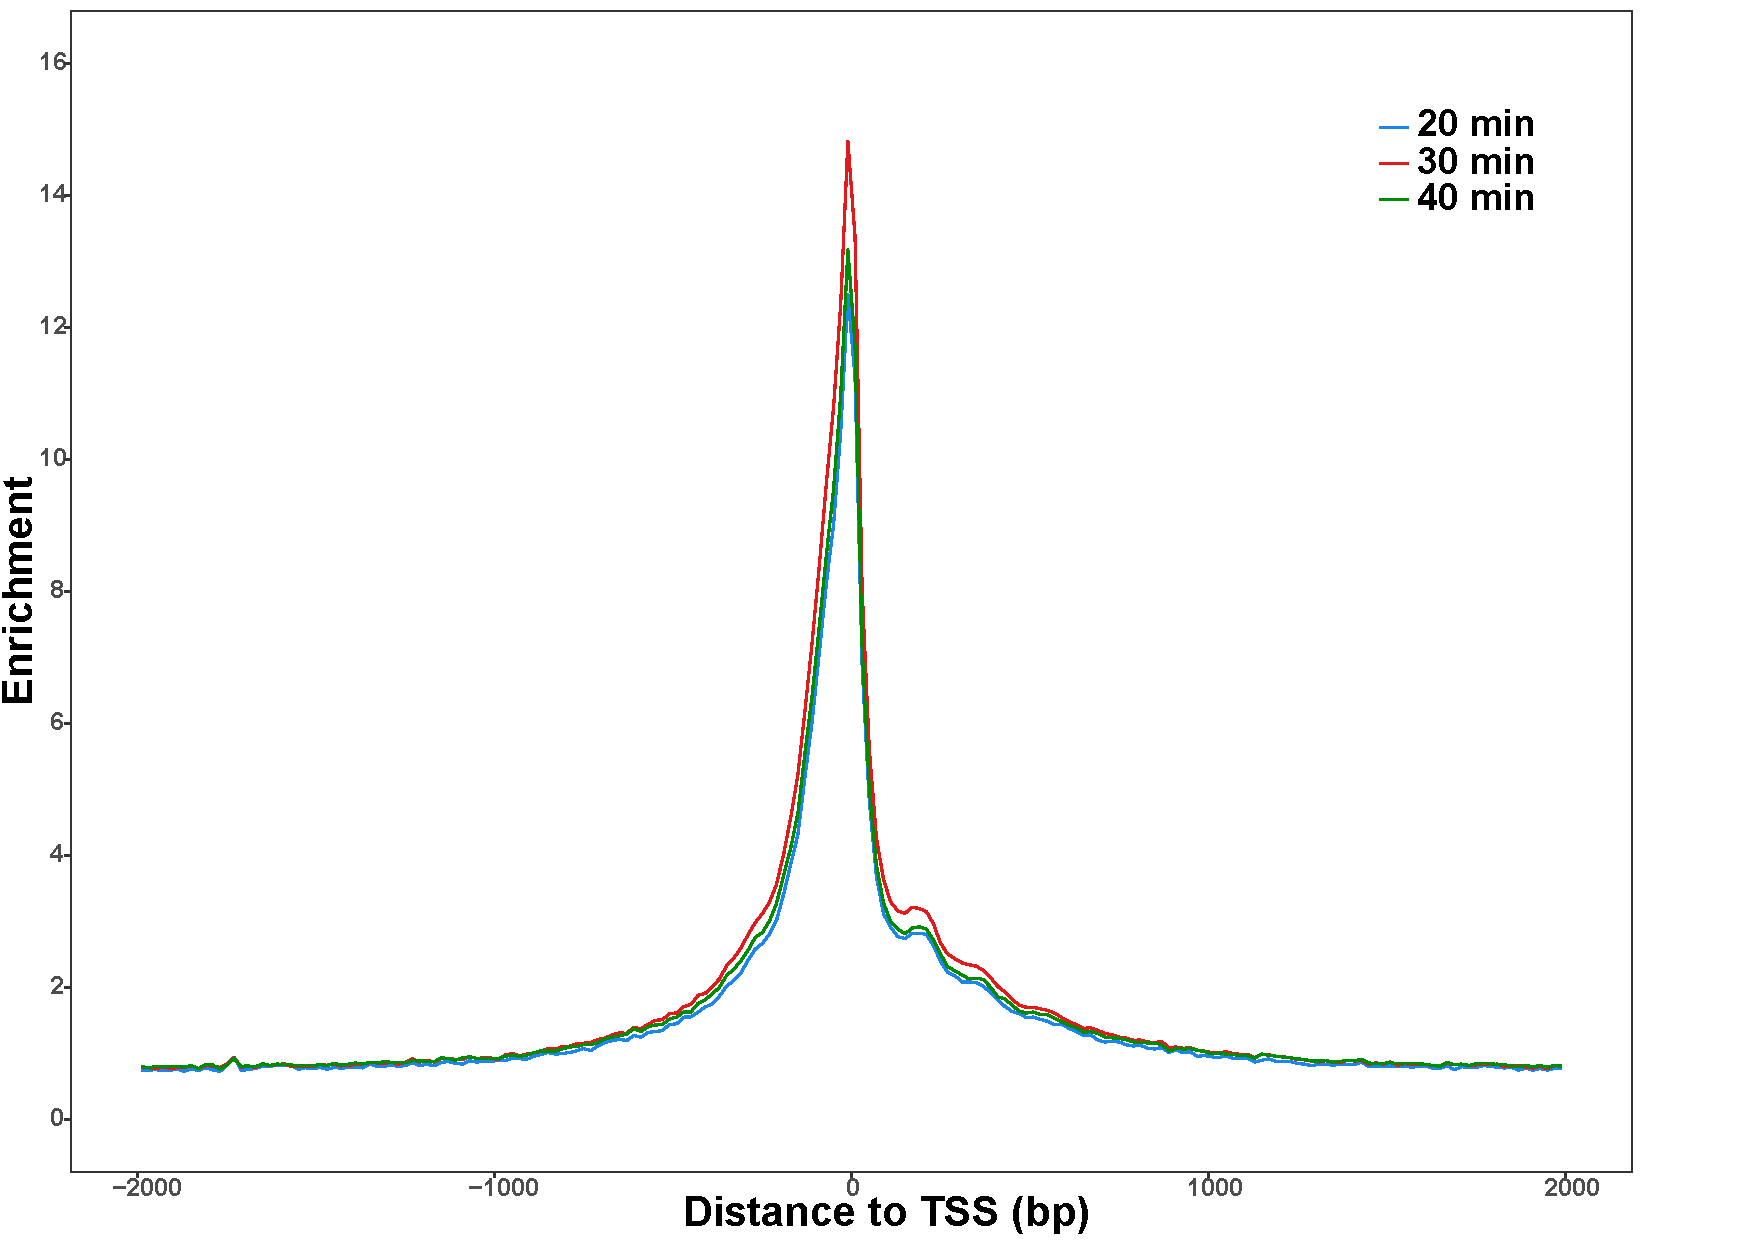
\includegraphics[width=\textwidth]{./Results1/pdfs/ATAC_optimisation_CD4_20_30_40_min_tss_enrichment}
	\caption{\textbf{}} % to add text to the figure name
\end{subfigure}
\caption[Assessment of the effect of transposition times on the ATAC-seq measurements]{\textbf{Assessment of the effect of transposition times on the ATAC-seq measurements}. (A) Representative plot of the ATAC-seq fragment sizes density distribution following 20, 30 and 40 min of transposition in CD8$^+$ cells. Changes across different transposition times in CD14$^+$ monocytes, CD4$^+$, CD8$^+$ and CD19$^+$ cells of (B) the ratio between ATAC-seq nucleosome-free fragments (NFF) (fragments $\leq$150bp) and mono-nucleosome bound fragments (mNBF) ($>$151bp) and (C) TSS fold-enrichment. (D) CD4$^+$ cells enrichment of ATAC-seq fragments for different transposition times across the TSS of all Ensembl genes.}
\label{figure:Transposition_times_ATAC}
\end{figure} 

This variation in NFF/mNBF did not significantly impact the signal-to-noise ratio, with the largest TSS enrichment values corresponding to 30 min in three cell types (Figure \ref{figure:Transposition_times_ATAC}C and D) and the major differences found across cell types. Differences between TSS fold-enrichments at 30 and 40 min were very modest and did not differ in more than four units in CD8$^+$ cells, where the largest variation was found. Before performing this formal comparison of transposition times, some sample recruitment had already been conducted using ATAC-seq with transposition for 40 min, as it was found to be the most appropriate condition based on the relative abundance of DNA fragment sizes profiles from the pre-sequencing library quality control. Although this analysis suggested 30 min as the best condition for the majority of the cell types tested in this single repetition, the differences between 30 min and 40 min were minor and therefore for consistency across the cohort 40 min was used for all other patient samples using ATAC-seq. 




\subsection{Comparison of ATAC-seq with Fast-ATAC protocol}
\label{Fast_ATAC}

An improved Fast-ATAC protocol from Corces and colleagues \parencite{Corces2016} was reported whilst the work in this thesis was being undertaken and was compared with the ATAC-seq protocol from Buenrostro and colleagues \parencite{Buenrostro2013}. The aim was to confirm the two main reported advantages of Fast-ATAC, namely reduction of mitochondrial reads and signal enhancement, before implementing it as the replacement for the current ATAC-seq protocol in use to process patient and control samples (Chapter \ref{ch:Results2} cohort 1A in Tables \ref{tab:Summary_all_cohorts}, \ref{tab:Psoriasis_cohort_metadata} and \ref{tab:Control_cohort_metadata}). Fast-ATAC was conducted in one healthy volunteer sample included in cohort 1B from Chapter \ref{ch:Results2} (Tables \ref{tab:Summary_all_cohorts} and \ref{tab:Control_cohort_metadata}). Fast-ATAC was specifically optimised for haematopoietic cells and used 30 min of transposition. Thus, for consistency, Fast-ATAC samples were here compared to the ATAC-seq library from Section \ref{ATACseq} transposed for 30 min in the same four cell types.


\begin{figure}[htbp]
\centering
\begin{subfigure}{0.5\textwidth}
\centering
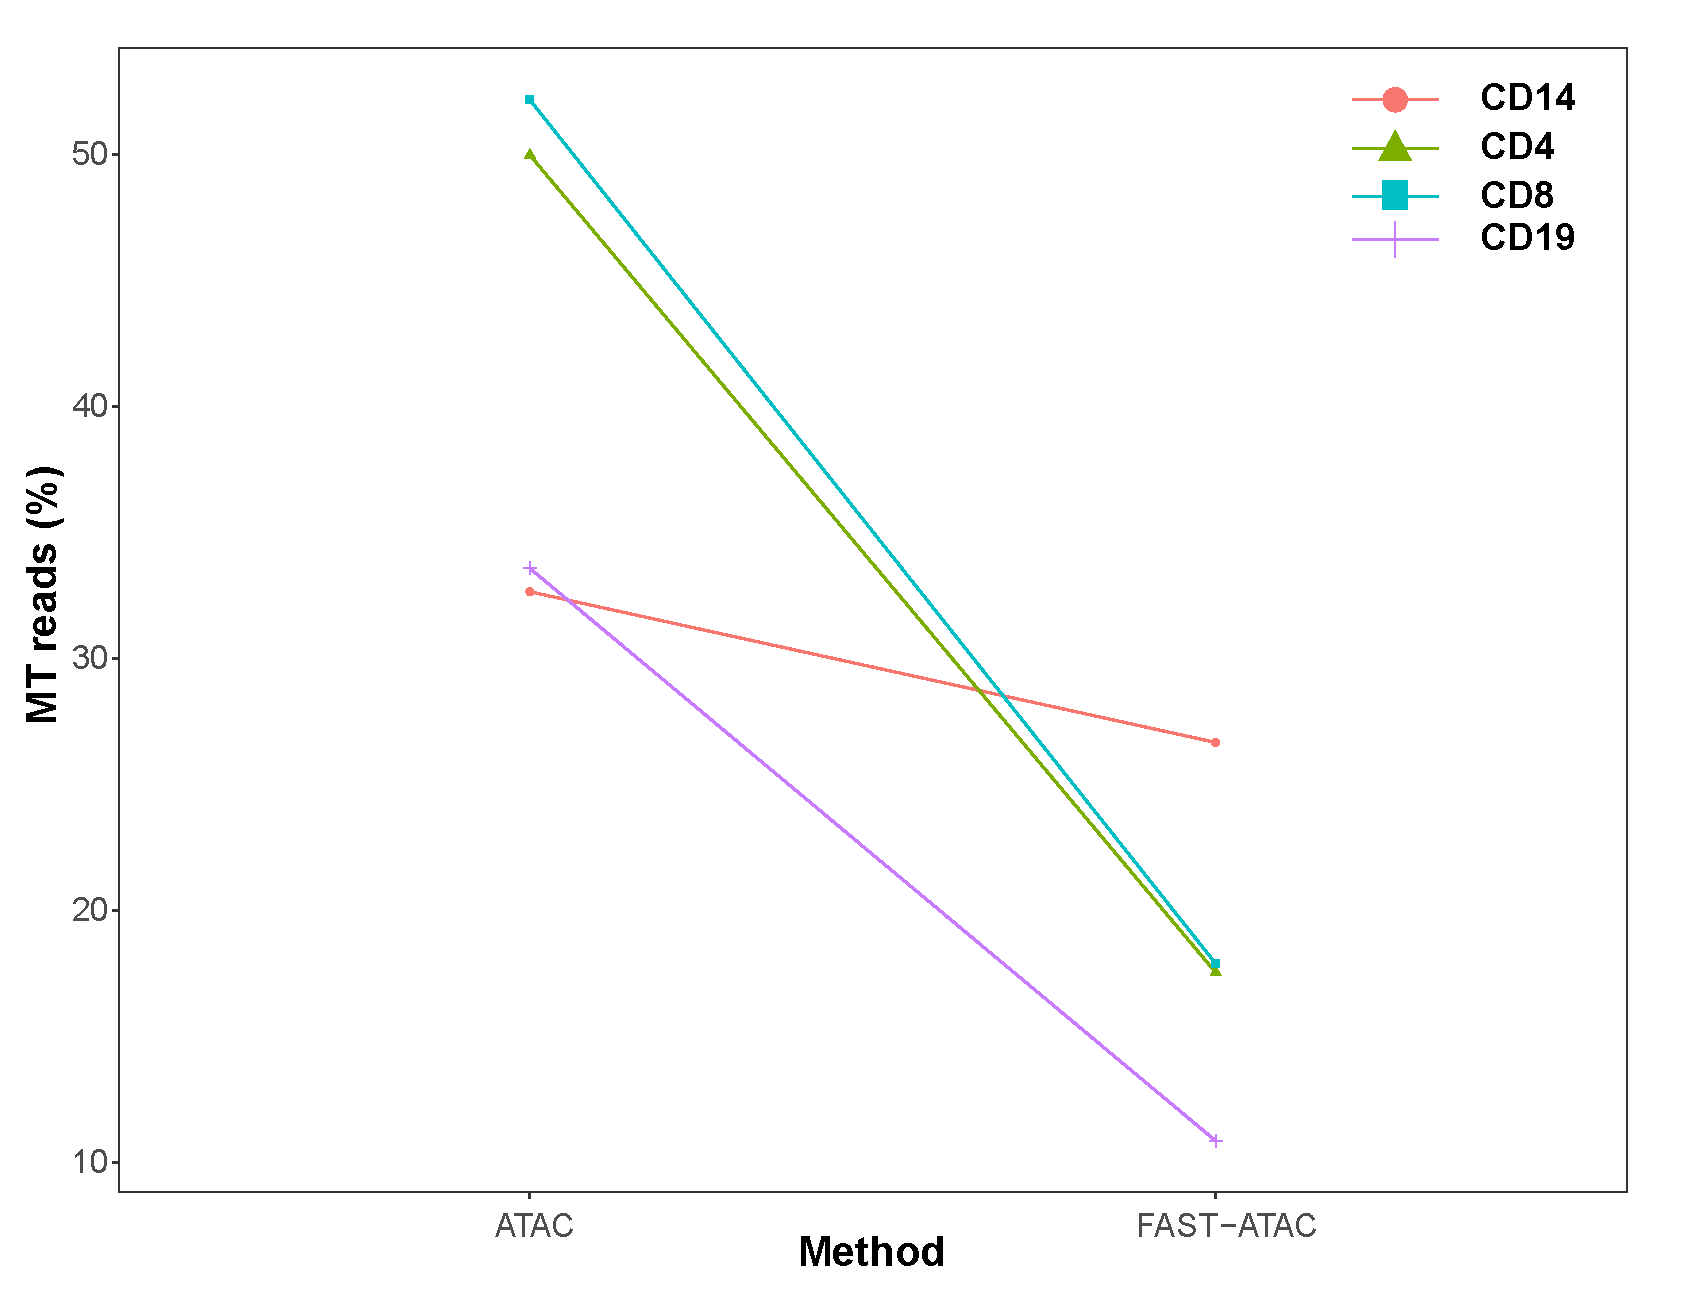
\includegraphics[width=\textwidth]{./Results1/pdfs/ATAC_vs_FAST_ATAC_percnt_MT_reads_dotplot}
\caption{\textbf{}}
% The percentage sign indicated that the other subfig goes side by side
\end{subfigure}%
\begin{subfigure}{0.5\textwidth}
\centering
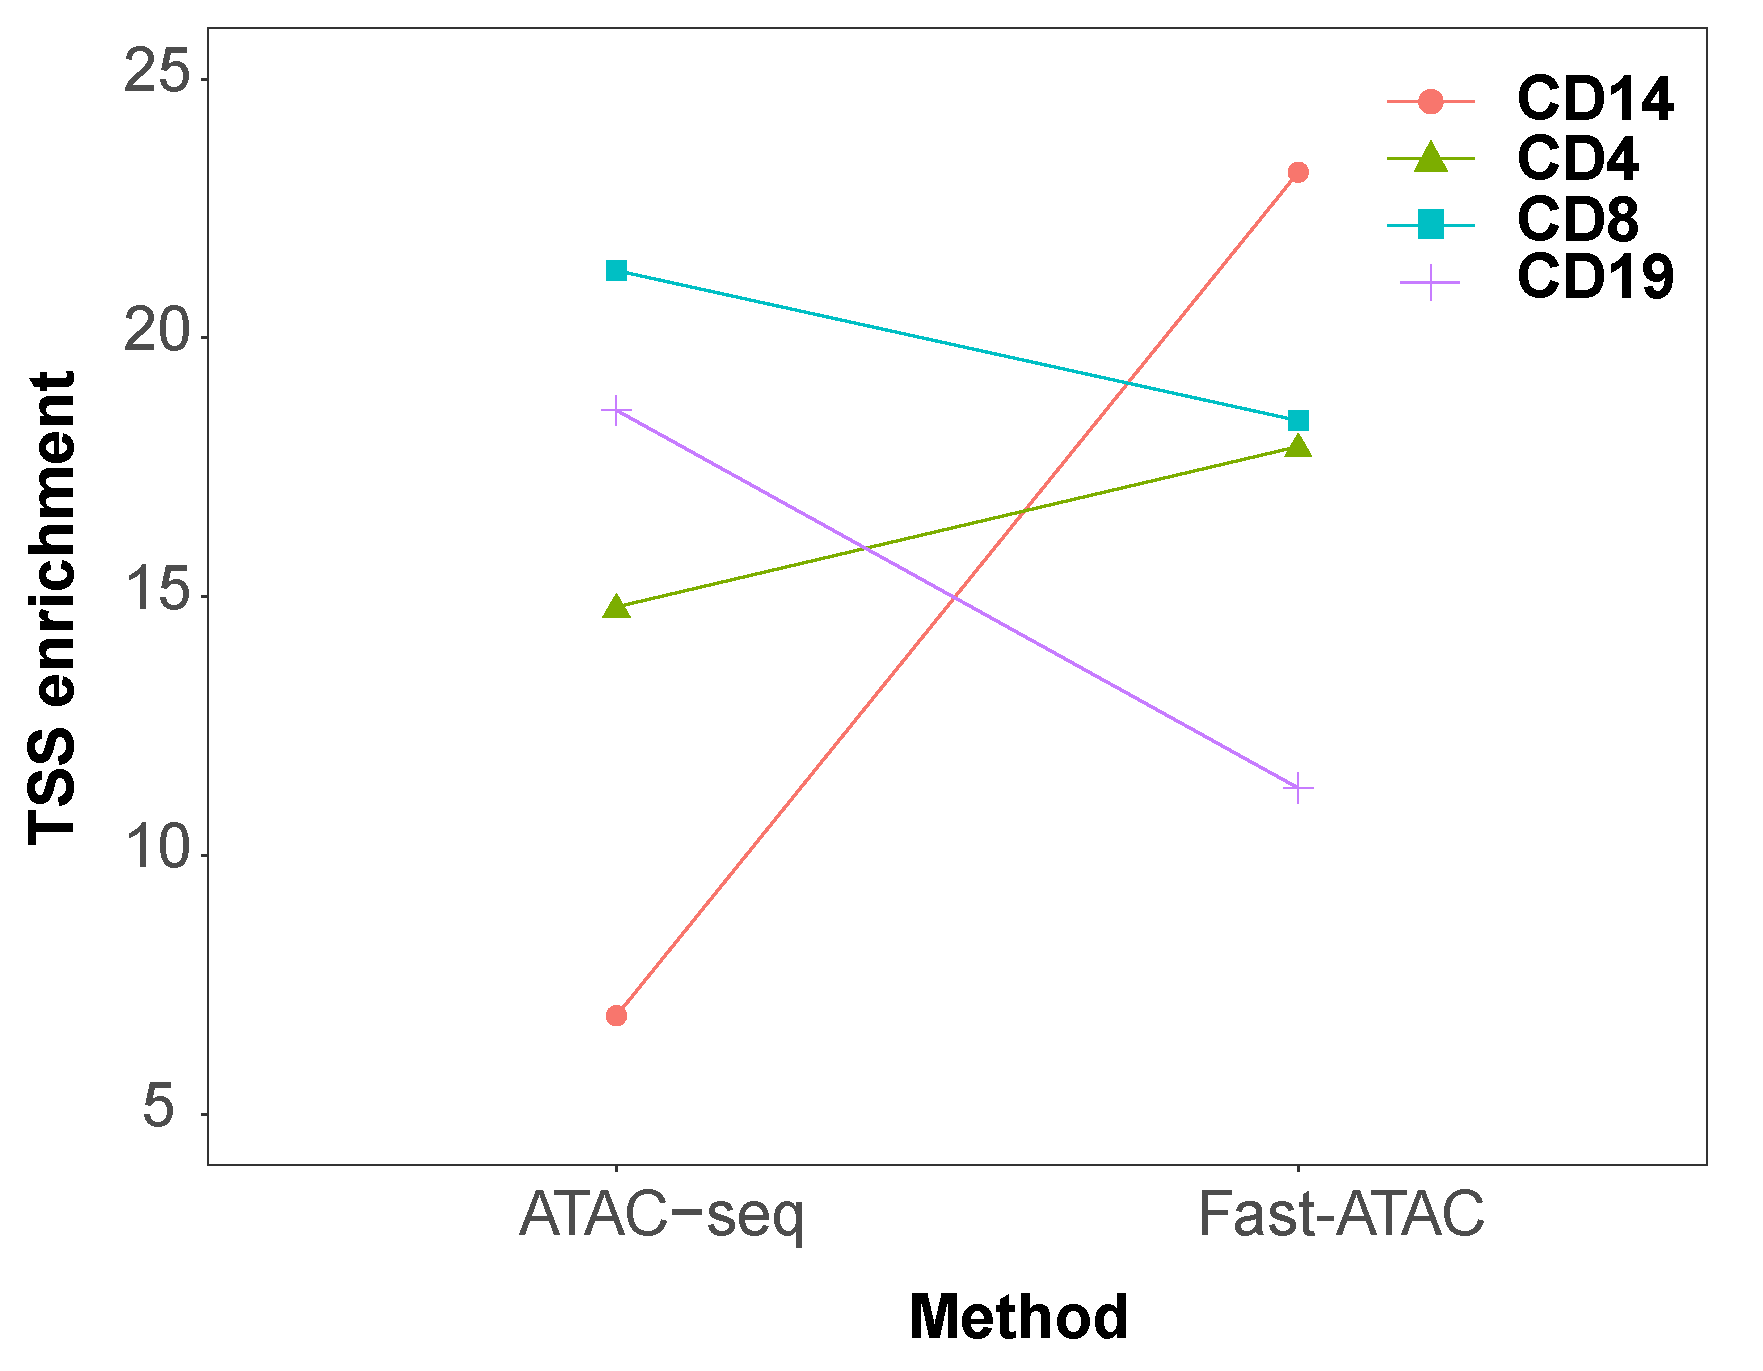
\includegraphics[width=\textwidth]{./Results1/pdfs/ATAC_vs_FAST_ATAC_tss_dotplot}
\caption{\textbf{}}
\end{subfigure}
\caption[Differences in mitochondrial DNA abundance and TSS enrichment between ATAC-seq and Fast-ATAC protocols.]{\textbf{Differences in mitochondrial DNA abundance and TSS enrichment between ATAC-seq and Fast-ATAC protocols.} Representation of changes in (A) percentage of mitochondrial reads and (B) TSS fold-enrichment between ATAC-seq and Fast-ATAC libraries for CD14$^+$ monocytes, CD4$^+$, CD8$^+$ and CD19$^+$ cells. Fast-ATAC protocol was specifically optimised by Corces and colleagues for hematopoietic cells and recommends 30 min of transposition (\ref{ch:Mat} and Corces \textit{et al.} 2016). Therefore, for consistency, Fast-ATAC samples were compared to the ATAC-seq libraries from Section \ref{ATACseq} transposed for 30 min.}
\label{figure:ATAC_vs_FAST_ATAC}
\end{figure} 

%\ToDo{Prospective analysis comparing all the ATAC-seq vs the Fast-ATAC libraries generated by the end of this thesis (samples presented in Chapters \ref{ch:Results2} and \ref{ch:Results3}) only showed a significant increase in TSS fold-enrichment for the Fast-ATAC protocol in CD4${^+}$ T cells (unpaired Wilcoxon signed-ranked test p-value=0.024) (Figure  \ref{figure:Comparison_ATACseq_vs_fastATAC_all_thesis_samples}A). Conversely, Fast-ATAC significantly reduced the percentage of mitochondrial reads in the four studied cell types (unpaired Wilcoxon signed-ranked test p-values$<$4.1x10$^{-05}$) (Figure  \ref{figure:Comparison_ATACseq_vs_fastATAC_all_thesis_samples}B).}


The percentage of mitochondrial reads in the Fast-ATAC libraries was lower for all cell types analysed compared to ATAC-seq (Figure \ref{figure:ATAC_vs_FAST_ATAC}A). CD4$^+$ and CD8$^+$ cells showed the largest reduction from 50\% to less than 20\% when using ATAC-seq and Fast-ATAC, respectively. With regard to the background signal, differing trends were observed across cell types (Figure \ref{figure:ATAC_vs_FAST_ATAC}B). Improvement in TSS enrichment was observed for CD14$^+$ monocytes and CD4$^+$ T cells whereas CD8$^+$ and CD19$^+$ cells showed a reduction when using Fast-ATAC compared to ATAC-seq in this single repetition. Overall, the large decrease in mitochondrial reads together with the reduced duration of the experimental protocol supported the replacement of ATAC-seq by Fast-ATAC for future patients recruitment (see Chapter \ref{ch:Results2}). 




\subsection{Limitations of ATAC-seq and Fast-ATAC to assess chromatin accessibility in keratinocytes}
A particular aim of this thesis was to characterise the regulatory landscape in psoriatic keratinocytes, one of the most relevant cell types in this pathophysiology. In order to assess the feasibility of using the ATAC-seq protocol from Buenrostro and colleagues \parencite{Buenrostro2013} (referred to as ATAC 1 in this subsection), epidermis from a psoriatic lesional skin biopsy was isolated, digested with trypsin and filtered through a cell strainer to ensure a single-cell suspension, as detailed in Chapter \ref{ch:Mat}. Cell suspensions obtained from skin biopsies using trypsinisation of the epidermal layer are enriched in keratinocytes, constituting approximately 90\% of the cells \parencite{Haftek1986}.  Approximately 50,000 cells from the suspension were counted and ATAC 1 was performed for two different transposition times (30 and 40 min). %Given the challenge of handling skin biopsies and isolating the epidermis from psoriatic lesional skin, testing the performance of ATAC1 in the clinical sample of interest was considered the best approach.

 Pre-sequencing library quality control to assess the relative abundance of different DNA fragment sizes recapitulated the characteristic ATAC nucleosome pattern every $\sim$200bp resulting from transposition of nucleosome-free and nucleosome-bound DNA in both samples (Figures \ref{figure:PS02_skin_ATAC_QC_assessment}A and \ref{figure:PS2_40min_tapestation}). Following sequencing, calculation of TSS fold enrichment values for the two ibraries demonstrated to be below the acceptable cut-off threshold of 6, with slightly better signal (3.5 fold-enrichment) for the 30 min transposition time (Figure \ref{figure:PS02_skin_ATAC_QC_assessment}B). Fragment size distribution using NGS data from the same libraries was consistent with the pre-sequencing assessment, showing approximately equal abundance of the NFF and mono-nucleosome fragments for both transposition times (Figure \ref{figure:PS02_skin_ATAC_QC_assessment}C). Approximately similar abundance of NFF and NBF can also be found in good quality libraries with TSS fold-enrichment above 6 (as seen previously). However, in this case, the extremely low TSS enrichments could suggest that a significant proportion of the NFF in these libraries are free-DNA released by apoptotic cells as a result of the trypsinisation step. Moreover, poor lysis of the keratinocytes may also result in inefficient access of the transposase into the nuclei compartment. This would cause under-transposition and greater NBF abundance when compared to NFF, which in this case may not be revealed as a result of large amounts of NFF being generated from tagmented free-DNA.



\begin{figure}[htbp]
\centering
\begin{subfigure}{0.7\textwidth}
\centering
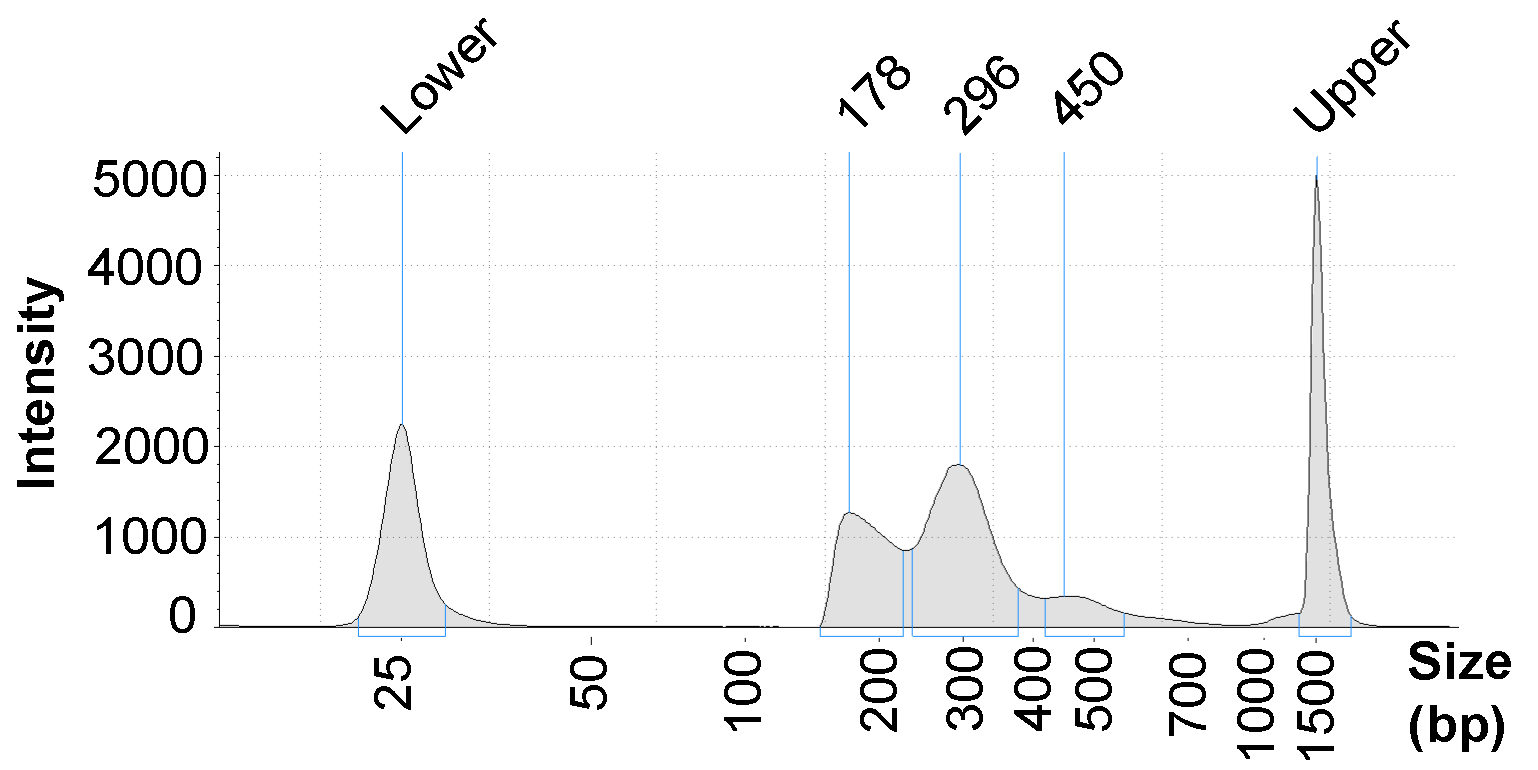
\includegraphics[width=\textwidth]{./Results1/pdfs/ATAC_PS02_tapestation_30min}
\caption{\textbf{}}
\end{subfigure}
\begin{subfigure}{0.45\textwidth}
\centering
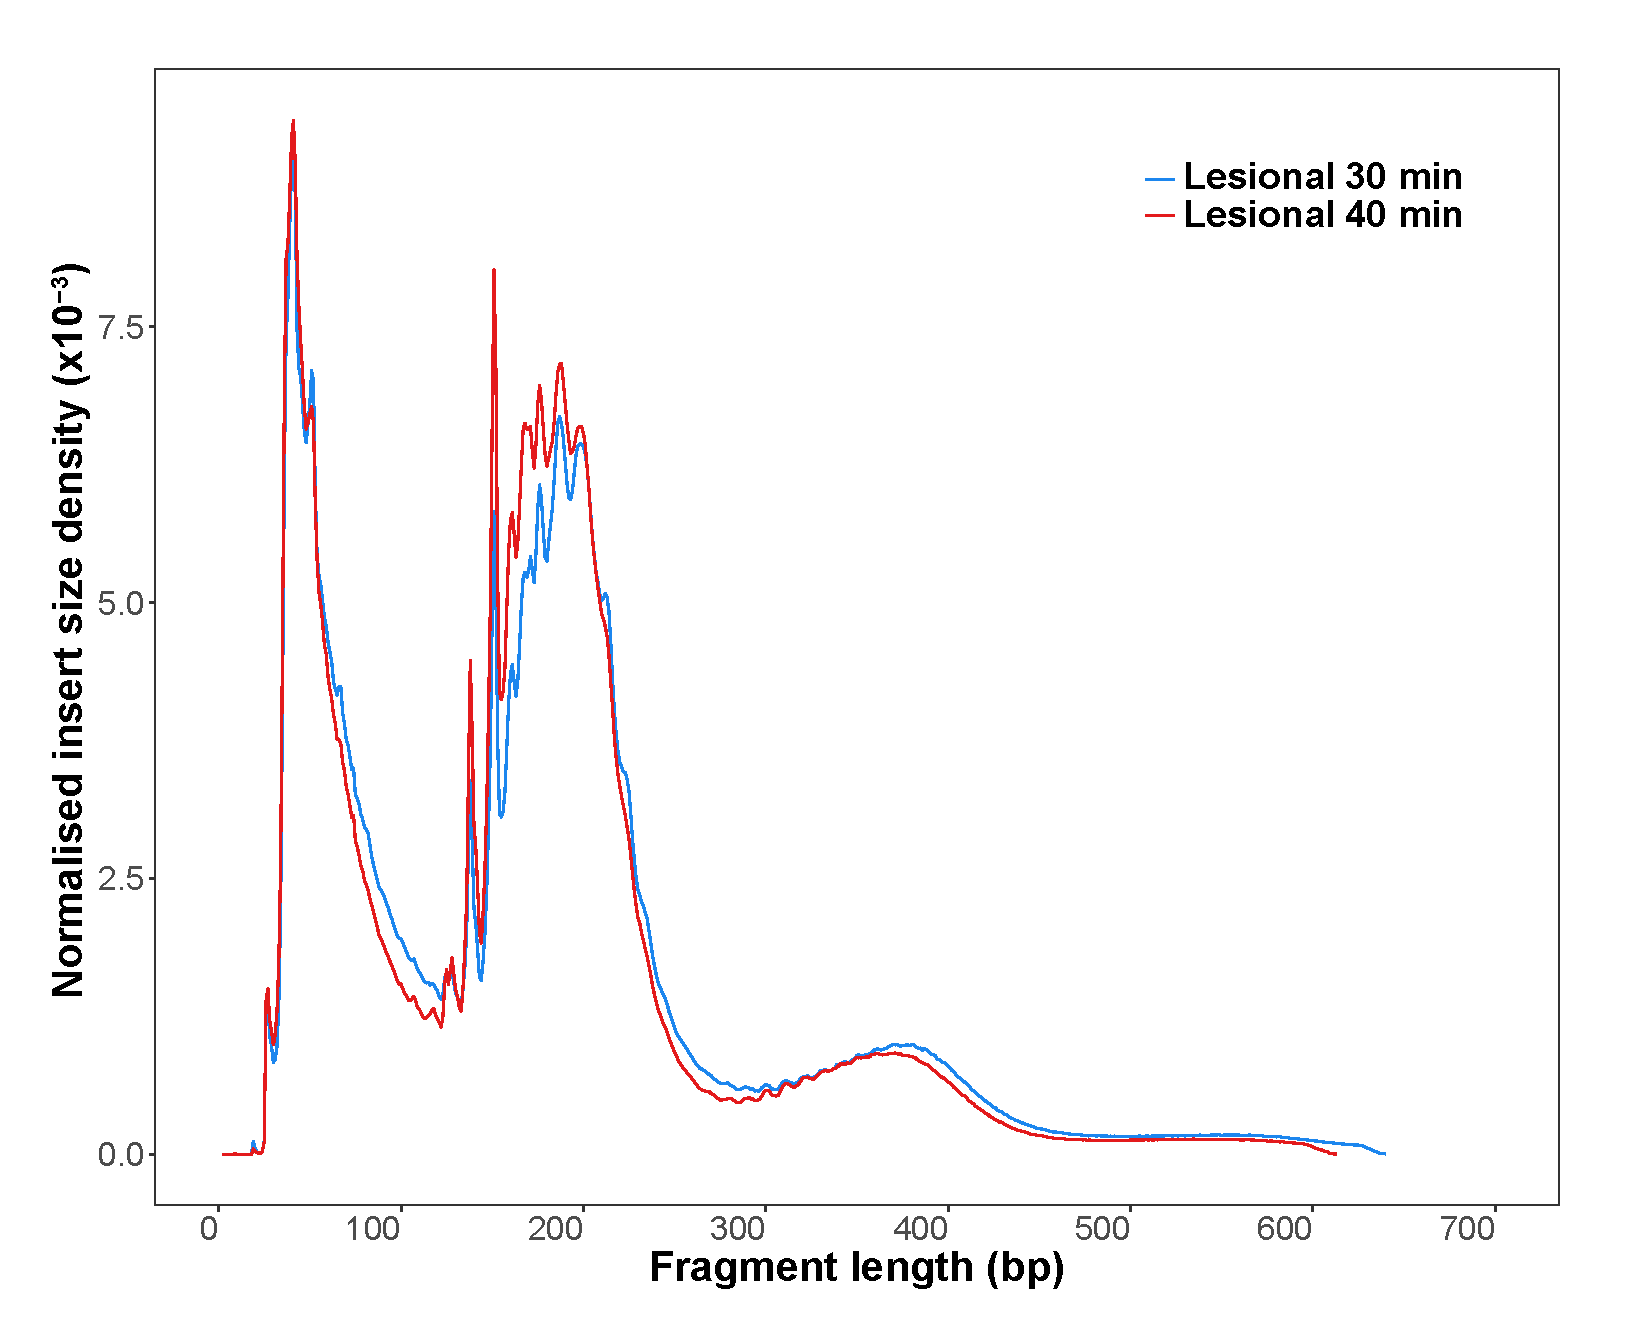
\includegraphics[width=\textwidth]{./Results1/pdfs/ATAC_PS-2_30_40_min_fragment_size_distribution}
\caption{\textbf{}}
\end{subfigure}%
\begin{subfigure}{0.45\textwidth}
\centering
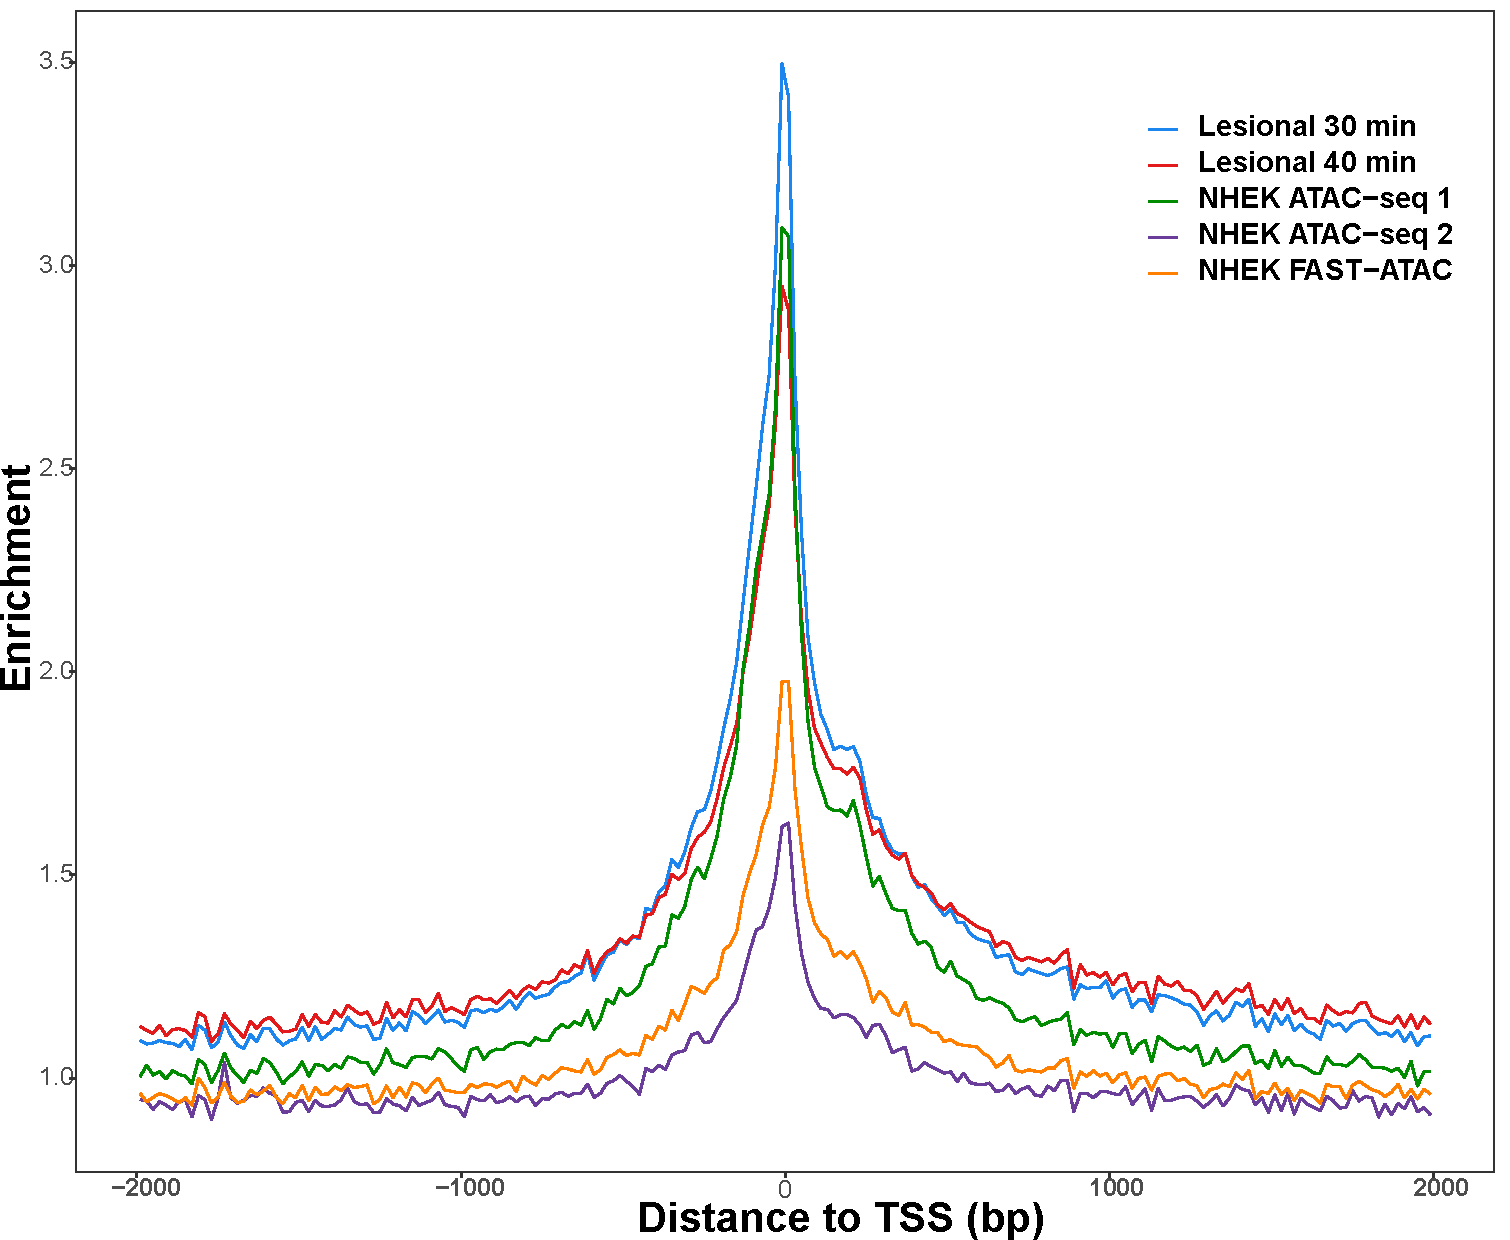
\includegraphics[width=\textwidth]{./Results1/pdfs/ATAC_skin_TSS_enrichment_PS02_30_40min_NHEK_ATAC1_ATAC_2_FAST_ATAC}
\caption{\textbf{}} % to add text to the figure name
\end{subfigure}
\caption[Quality control assessment of different ATAC protocols in keratinocytes from a psoriatic lesion and NHEKs.]{\textbf{Quality control assessment of different ATAC protocols in keratinocytes from a psoriatic lesion and NHEKs.} (A) Pre-sequencing quality control showing relative abundance of different DNA fragment sizes in the ATAC libraries generated in 50,000 cells from a suspension of keratinocytes isolated from lesional skin of one psoriasis patient. Cells from the same suspension were used to test two transposition times (30 and 40 min) and the profile for the 30 min library is shown here. The corresponding pre-sequencing profile for the sample transposed for 40 min is included in Figure \ref{figure:PS2_40min_tapestation}. (B) Fold-enrichment of ATAC fragments across the Ensembl annotated TSS from the ATAC 1 psoriasis lesional keratinocytes libraries, previously mentioned in (A), and NHEK libraries generated by performing ATAC 1, ATAC 2 and Fast-ATAC protocols directly on adherent cells cultured in 96-well plates. (C) Density distribution of sequenced fragments for ATAC 1 libraries in (A) and Figure \ref{figure:PS2_40min_tapestation}.}
\label{figure:PS02_skin_ATAC_QC_assessment}
\end{figure} 


Following the ATAC-seq protocol, a modified ATAC-seq version for keratinocytes by Bao and colleagues (named ATAC 2 in this subsection) and the Fast-ATAC protocols were published \parencite{Bao2015, Corces2016}. Interestingly, Bao's protocol was performed directly on NHEKs adhered to the cell culture plate, avoiding the trypsinisation step that could compromise cell viability. This protocol reduced the percentage of NP-40 (weaker lysis) but increased the amount of Tn5 enzyme per cell, which may address potential under-transposition due to insufficient Tn5 availability. In line with Bao and colleagues approach (avoiding trypsinisation), the three ATAC protocols (ATAC 1 30 min, ATAC 2 and Fast-ATAC using C1 conditions, Table \ref{tab:ATAC_skin_optimisation_protocols}) were tested directly on keratinocytes isolated from skin biopsies and/or NHEKs cultured on 96-well plates to avoid the trypsinisation step and the subsequent impact of dead cells in data quality. For this purpose, the cell suspension of epidermal keratinocytes obtained from skin biopsies were cultured for 3h in a 96-well plate following a washing step to remove remaining non-viable cells. This procedure is known as adherence assay and allows the isolation of viable undifferentiated keratinocytes. Similarly, 50,000 NHEKs were cultured per well and used as control to test the performance of the different protocols in keratinocyte cells. 


\begin{table}[htbp]
%\setlength{\tabcolsep}{20pt}
%\renewcommand{\arraystretch}{1.5}
\begin{tabular}{@{} c c c}
\toprule
\textbf{Protocol}   & \textbf{Lysis and} & \textbf{Key parameters} \\
                    & \textbf{transposition} &  \\
\midrule
\midrule
ATAC 1          & Two steps & 0.1\% NP-40 and 2.5$\micro$L Tn5  \\
\parencite{Buenrostro2013} && \\
&&\\
ATAC 2          &Two steps   & 0.05\% NP-40 and 5$\micro$L Tn5  \\
\parencite{Bao2015} &&\\
&&\\
                                 &             & C1$^\ast$: 0.01\% digitonin, 2.5$\micro$L Tn5 \\
 Fast-ATAC                       &             & C2: 0.01\% digitonin, 0.5$\micro$L Tn5 \\
\parencite{Corces2016}           & One step    & C3: 0.025\% digitonin, 0.5$\micro$L Tn5 \\
													       &             & C4: 0.025\% digitonin, 2.5 $\micro$L Tn5 \\
\bottomrule
\end{tabular}
\medskip %gap
\caption[Description of the most relevant parameter from the ATAC-seq and FAST-ATAC protocols assayed in NHEK and skin biopsies.]{\textbf{Description of the most relevant parameter from the ATAC-seq and FAST-ATAC protocols assayed in NHEK and skin biopsies.}Transposition times for all protocols was 30 min. $^\ast$ corresponds to the original Fast-ATAC conditions from Corces \textit{et al.} 2016.}
\label{tab:ATAC_skin_optimisation_protocols}
\end{table}
\bigskip %bigger space

For the three tested protocols, the NHEKs library size distribution of sequenced fragments showed presence of NFF but almost absent nucleosome pattern, particularly for the ATAC 2 protocol (Figure \ref{figure:Skin_ATAC1__ATAC2_Fast_ATAC_Omni_ATAC_QC_assessment}A). Moreover, the TSS enrichment was under the recommended cut-off of 6 in skin biopsy keratinocytes and NHEKs libraries from the three protocols (Figures \ref{figure:PS02_skin_ATAC_QC_assessment}C and \ref{figure:TSS_skin_biopsies}). Potential poor lysis was further addressed through additional modifications of the Fast-ATAC protocol by increasing the concentration of the detergent digitonin (from 0.01\% in the published Fast-ATAC protocol to 0.025\%) in combination with standard or lower Tn5 amounts (2.5 and 0.5 $\micro$L, respectively)(Table \ref{tab:ATAC_skin_optimisation_protocols} C2 to 4). Library quality control prior to sequencing to assess the relative abundance of different DNA fragment sizes failed to show the characteristic nucleosome pattern profile expected in ATAC for any of the three tested conditions, and therefore NGS was not performed (Figure \ref{figure:NHEK_tapestation}A, B and C).

 

\begin{figure}[htbp]
\centering
\begin{subfigure}{0.48\textwidth}
\centering
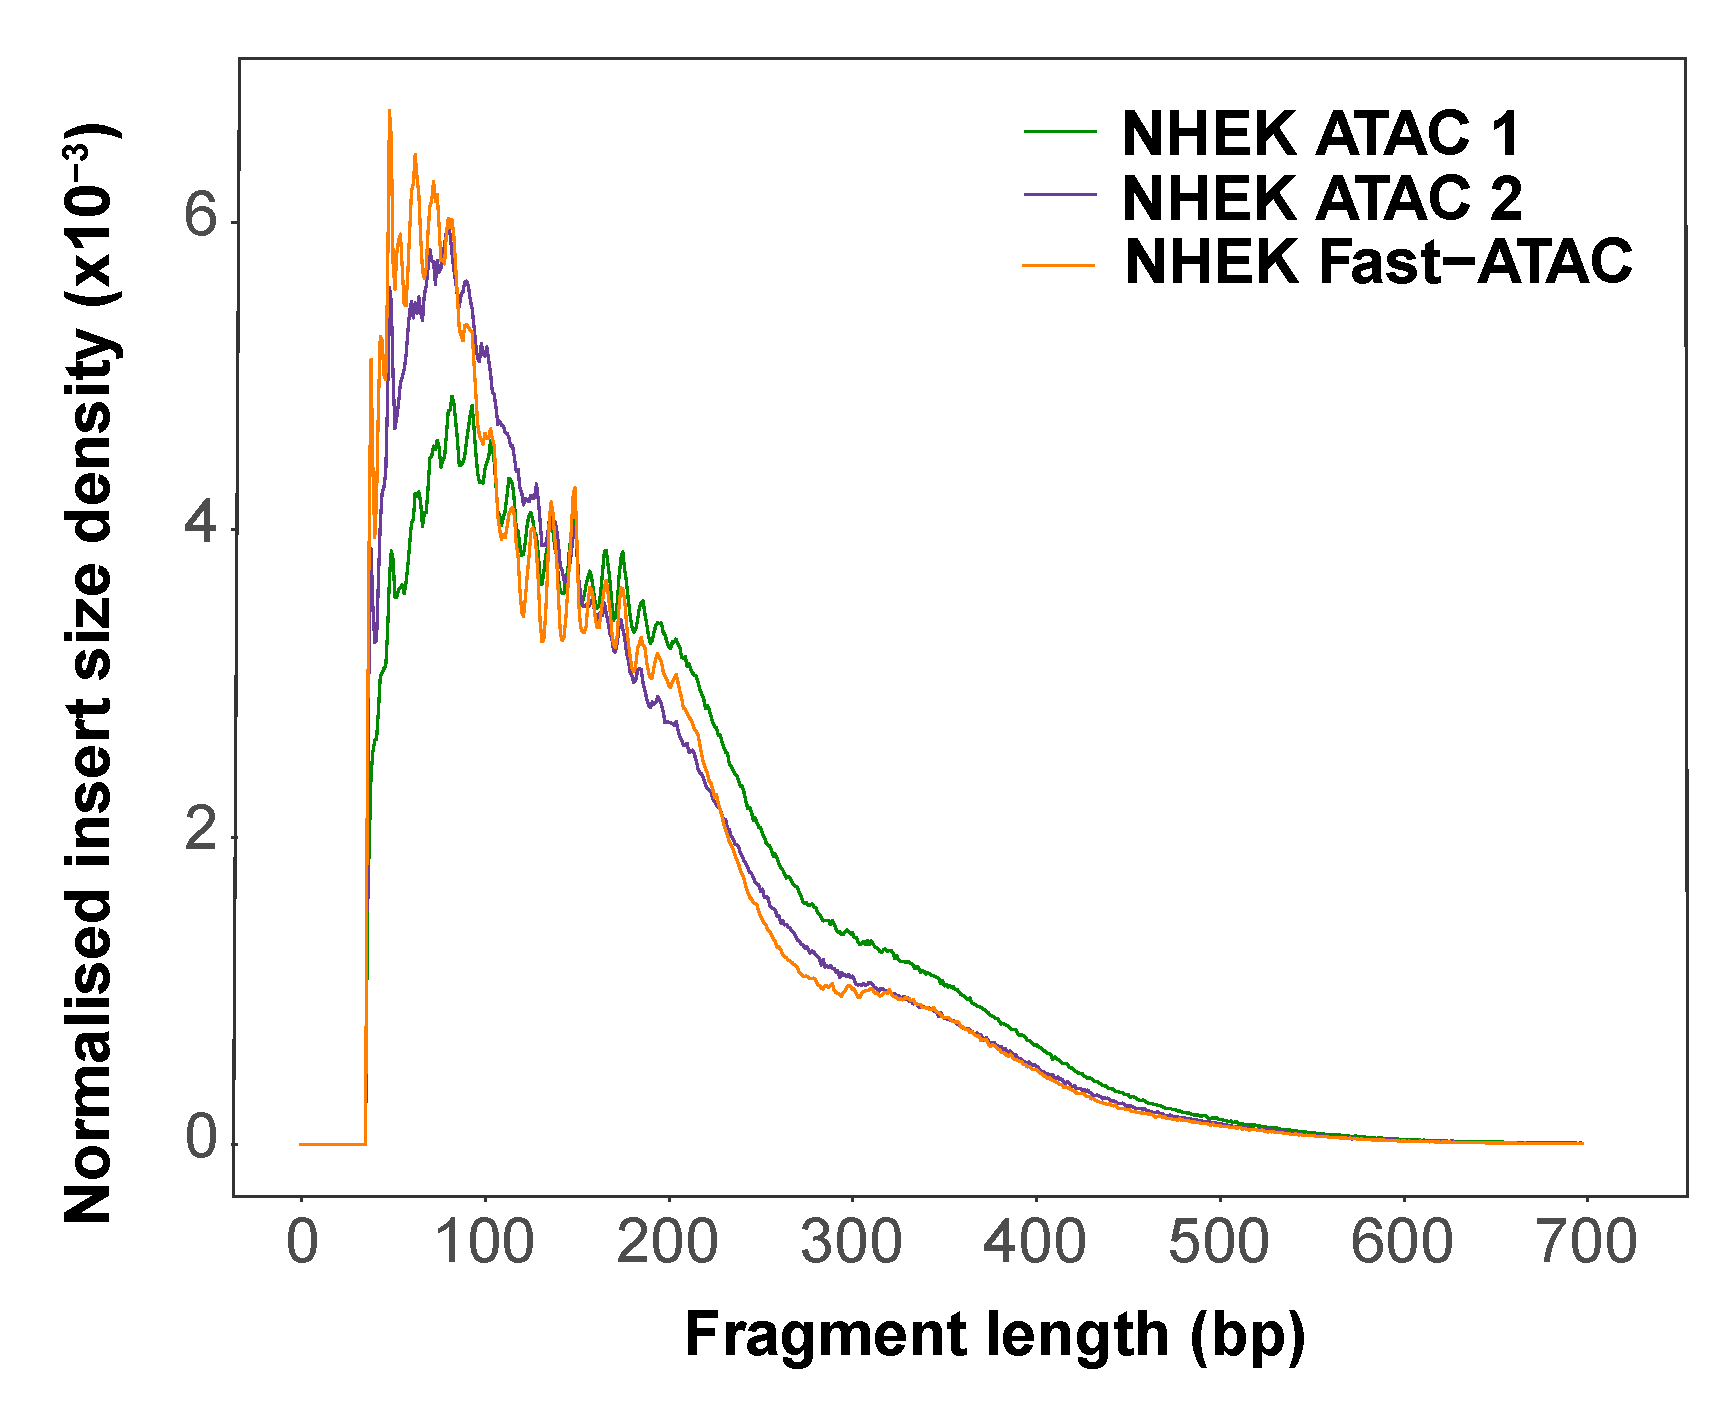
\includegraphics[width=\textwidth]{./Results1/pdfs/ATAC_NHEK_ATAC1_ATAC2_FAST_ATAC_fragment_size_distribution}
\caption{\textbf{}}
\end{subfigure}%
\begin{subfigure}{0.48\textwidth}
\centering
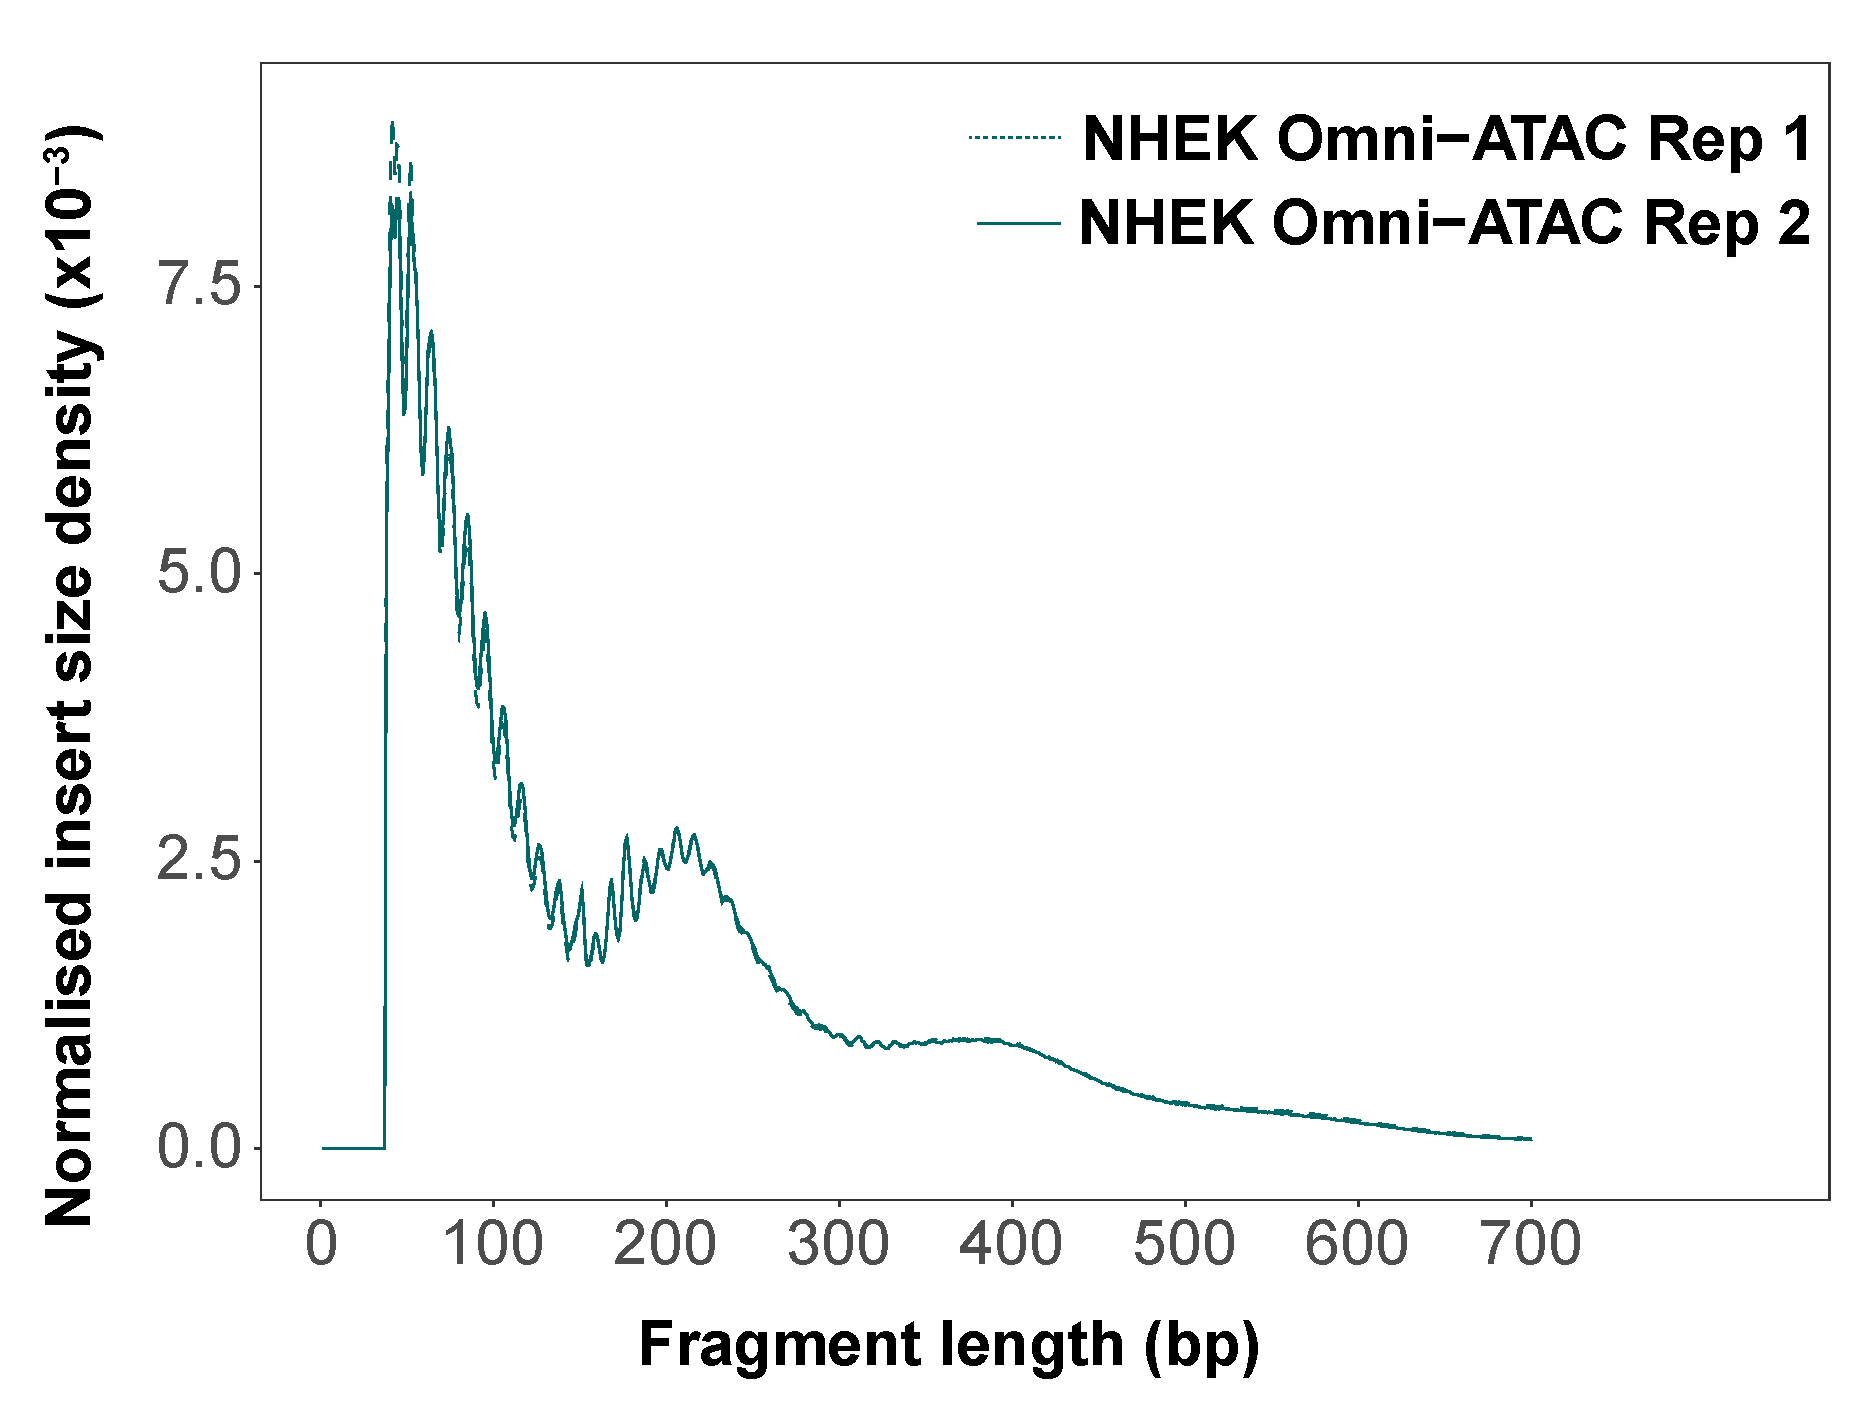
\includegraphics[width=\textwidth]{./Results1/pdfs/ATAC_NHEK_Omni_ATAC_fragment_size_distribution}
\caption{\textbf{}}
\end{subfigure}
\begin{subfigure}{0.5\textwidth}
\centering
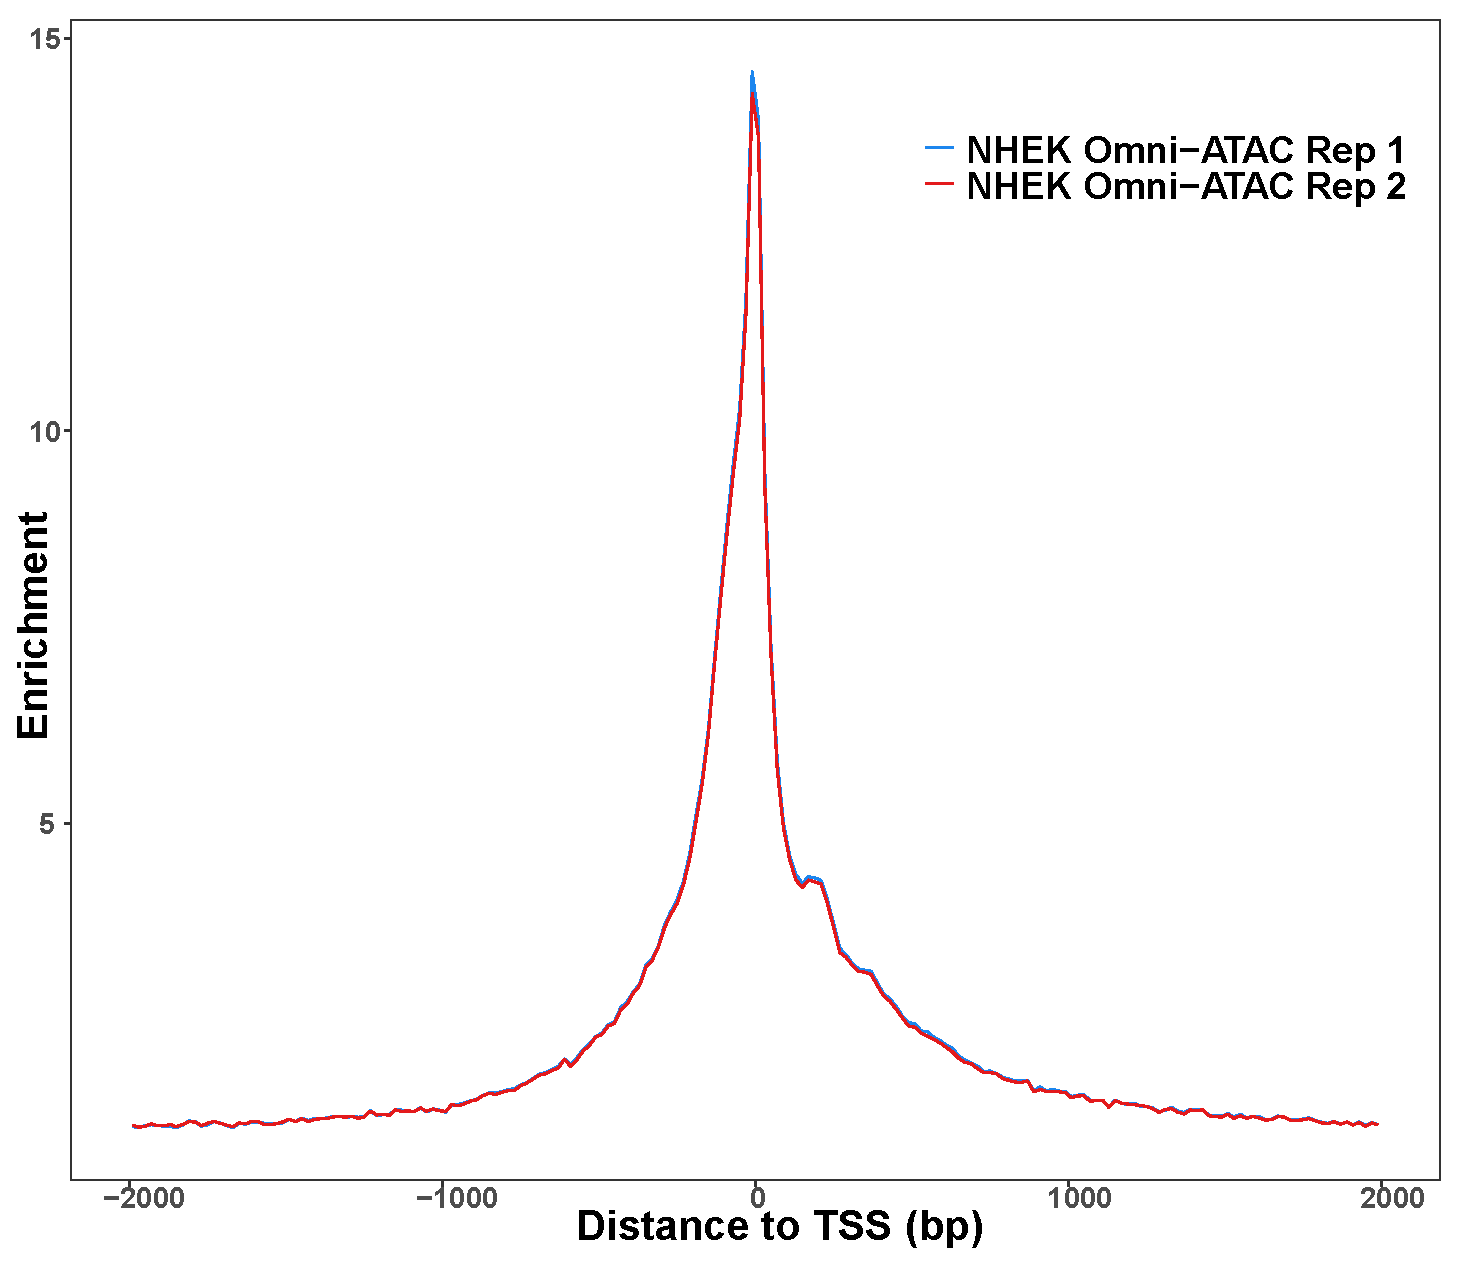
\includegraphics[width=\textwidth]{./Results1/pdfs/ATAC_skin_TSS_enrichment_NHEK_omni_ATAC}
\caption{\textbf{}} % to add text to the figure name
\end{subfigure}%
\caption[Quality control assessment of Fast-ATAC and Omni-ATAC in cultured NHEK]{\textbf{Quality control assessment of Fast-ATAC and Omni-ATAC in cultured NHEK.} Representation of the fragment sizes density distribution in NHEKs libraries generated using (A) ATAC 1, ATAC 2, Fast-ATAC or (B) Omni-ATAC protocols. (C) Fold-enrichment of ATAC fragments across the Ensembl annotated TSS from two Omni-ATAC technical replicates. In (A) the results for one of the two replicates is shown.}
\label{figure:Skin_ATAC1__ATAC2_Fast_ATAC_Omni_ATAC_QC_assessment}
\end{figure} 


At the end of the experimental work of this thesis, a new protocol called Omni-ATAC was published \parencite{Corces2017}. Omni-ATAC was a protocol suitable for every cell type, in contrast to ATAC 1 and Fast-ATAC, which were optimised for hematopoietic cells \parencite{Buenrostro2013,Corces2016}. Performance of this protocol in 50,000 viable NHEKs in suspension yielded the expected fragment size distribution for sequenced fragments, with the greatest abundance for NFF followed by mono and di-nucleosome fragments (Figure \ref{figure:PS02_skin_ATAC_QC_assessment}B). Moreover, high TSS enrichment values (approximately 15 fold change) were observed for the two replicates (Figure \ref{figure:PS02_skin_ATAC_QC_assessment}C). When performing overlap between the Omni-ATAC sample peaks filtered based on low stringency p-value (p-value=0.01) and the ENCODE DHSs from 125 cell types, the highest percentage of overlap (approximately 55\%) was observed for NHEKs (Figure \ref{figure:ATAC_skin_ENCODE_overlap_and_tracks}A). In contrast, the same analysis using peaks from the NHEKs libraries generated with ATAC 1, ATAC 2 and Fast-ATAC protocols only showed 20\% or less overlap of each sample called peaks with the ENCODE DHS data of the same cell type, supporting the higher quality and specificity of Omni-ATAC accessible regions in keratinocytes, even at a very low p-value filtering. The differences in the quality of ATAC signal between Omni-ATAC and the prior ATAC protocols was clearly observed at the keratin (\textit{KRT}) genes (main components of keratinocyte cytoskeleton) in chr17, where Omni-ATAC showed the lowest background noise, the highest signal intensity and the greatest number of high quality peaks (Figure \ref{figure:ATAC_skin_ENCODE_overlap_and_tracks}B). 

\begin{figure}[H]
\centering
\begin{subfigure}{0.40\textwidth}
\centering
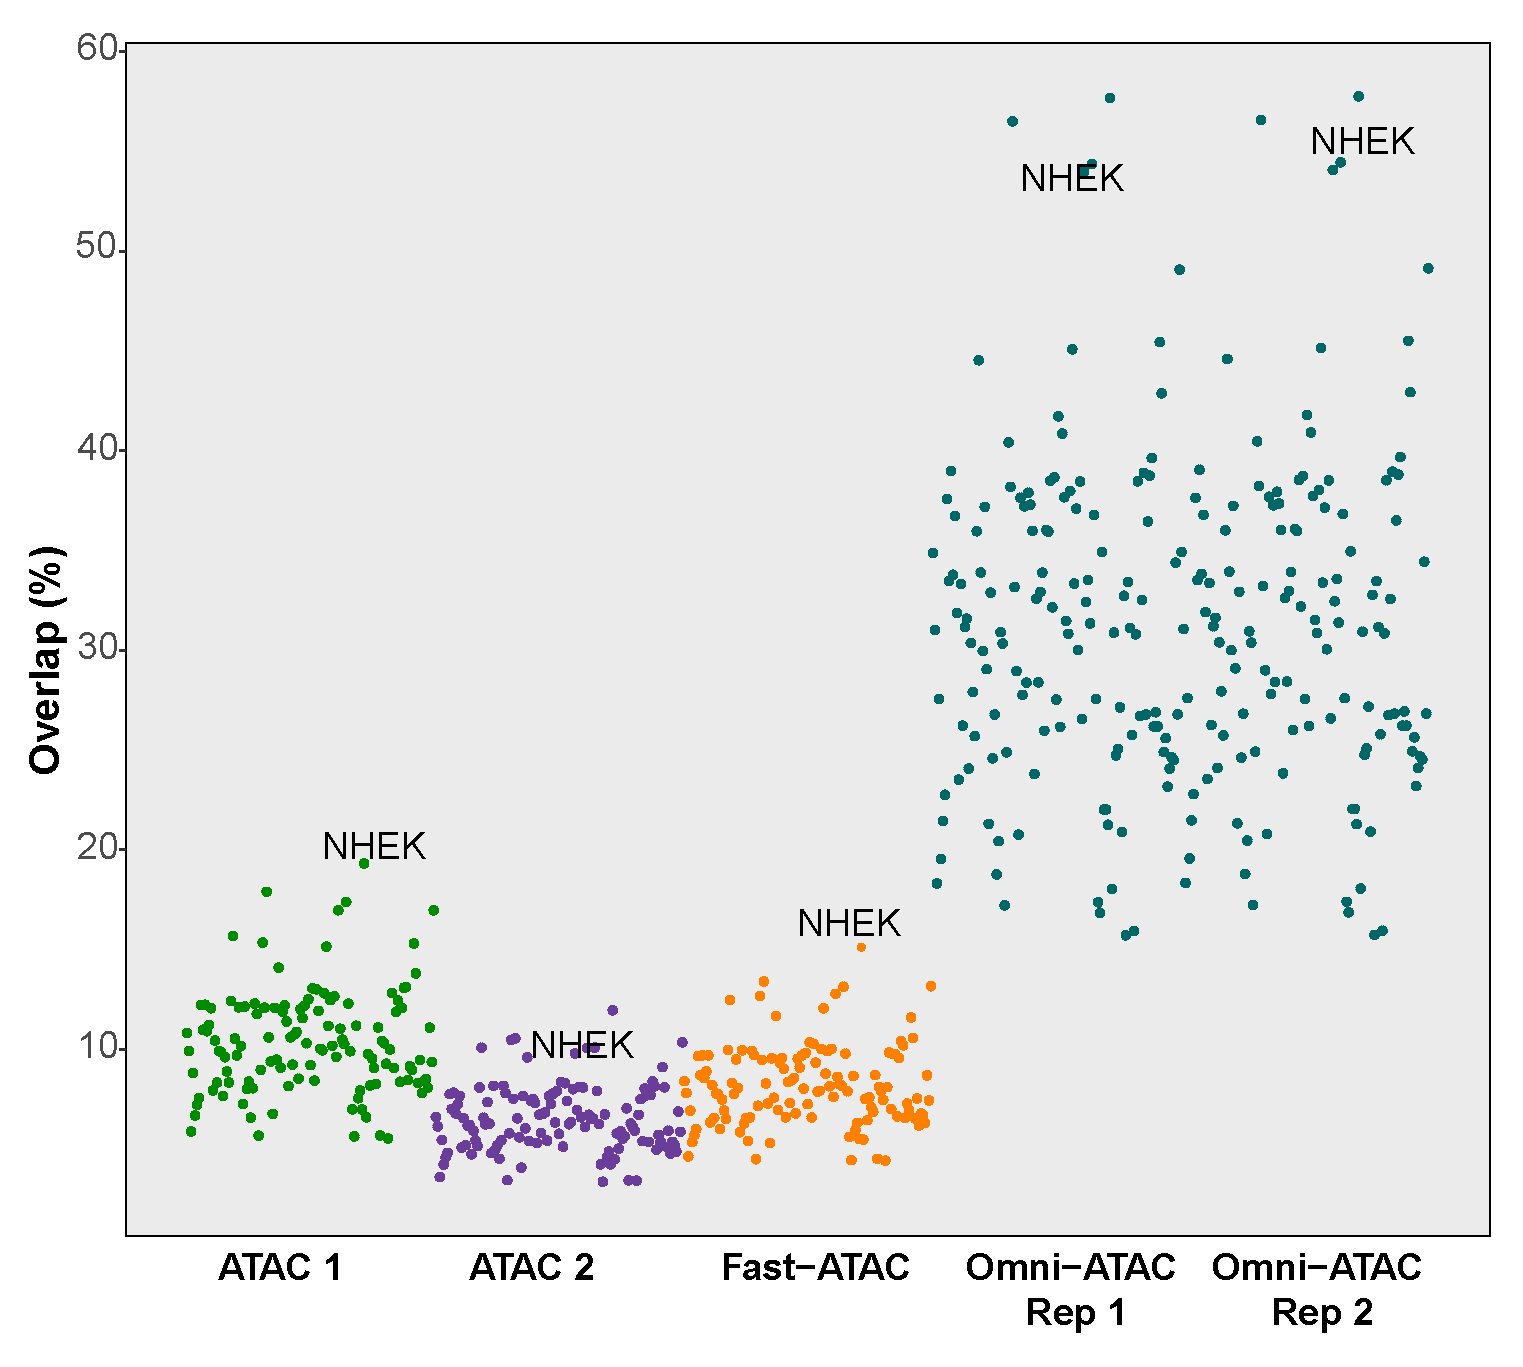
\includegraphics[width=\textwidth]{./Results1/pdfs/ENCODE_125_cell_types_overlap_FAST_ATAC_Omni_ATAC_pval_2}
\caption{\textbf{}}
% The percentage sign indicated that the other subfig goes side by side
\end{subfigure}
\begin{subfigure}{0.65\textwidth}
\centering
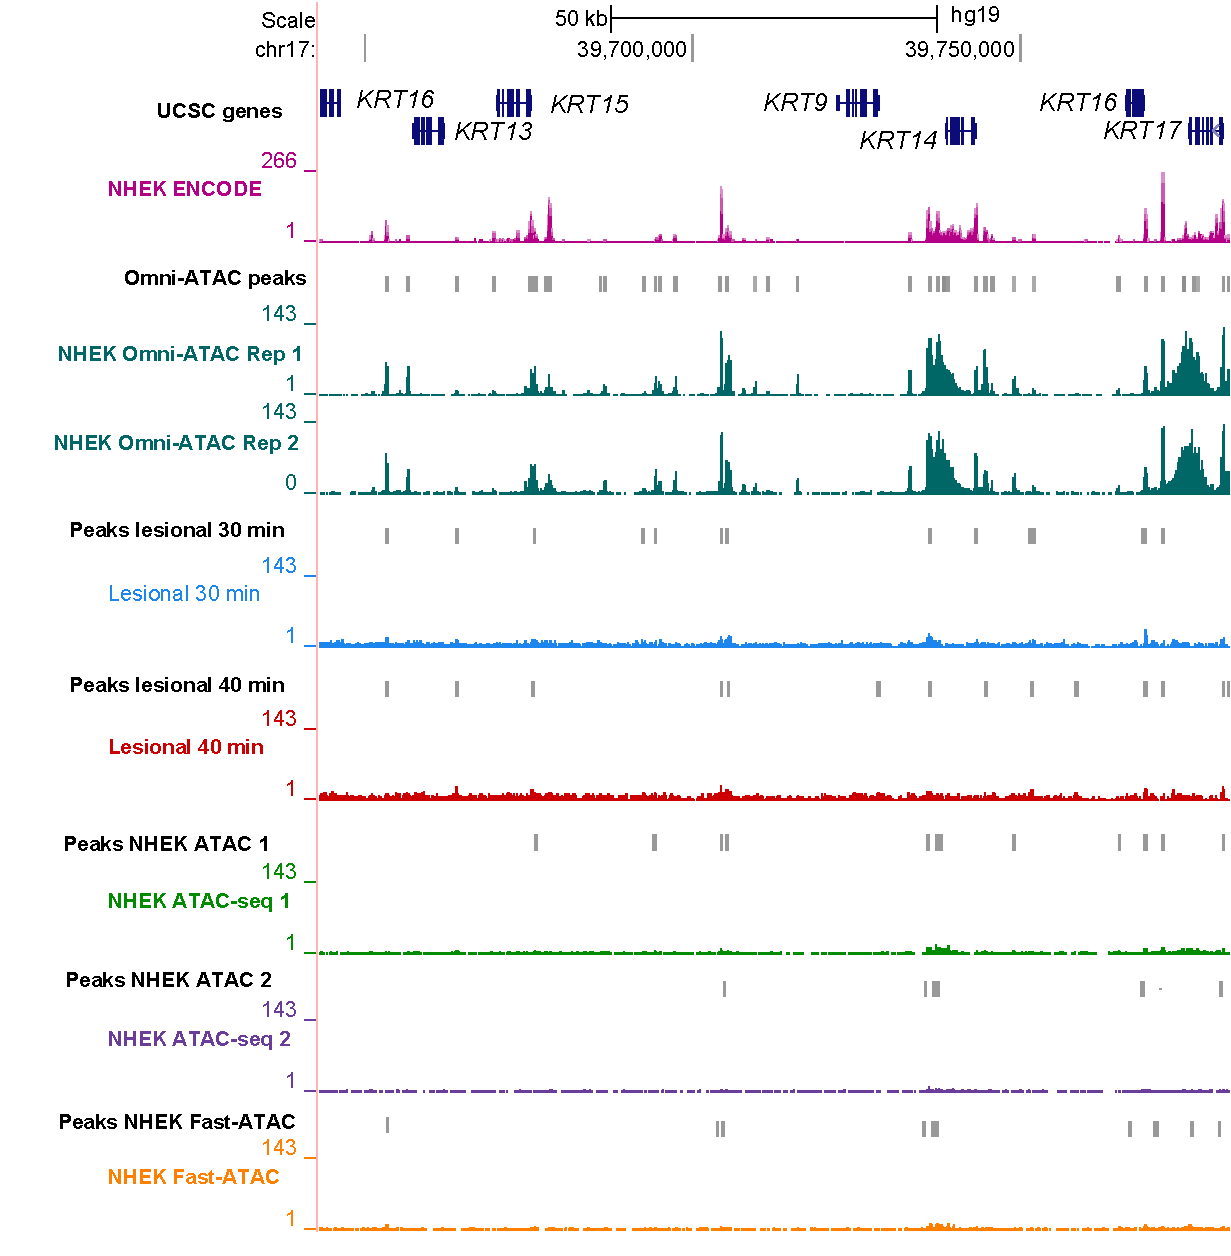
\includegraphics[width=\textwidth]{./Results1/pdfs/ATAC_skin_all_tracks_KRT}
\caption{\textbf{}}
\end{subfigure}
\caption[Comparison of 4 different ATAC protocols applied to psoriasis and/or healthy keratinocytes and NHEKs cells with published ENCODE DNase-seq data.]{\textbf{Comparison of four different ATAC protocols applied to psoriasis and/or healthy keratinocytes and NHEKs cells with published ENCODE DNase-seq data.} (A) Enrichment (\% of overlap) of observed peaks called in each ATAC sample (using low stringent p-value) with open DHS chromatin regions in 125 ENCODE cell types. (B) UCSC Genome Browser track showing ATAC read density (y-axis) at the chr17 keratin (KRT) family gene locus (x-axis) for different ATAC protocols (all subsampled to 30 million total reads).}
\label{figure:ATAC_skin_ENCODE_overlap_and_tracks}
\end{figure} 
\smallskip

 %Overall, this data was consistent with Corces \textit{et al.}, 2017, where consistent successful results in NHEKs were shown, and it encourages future testing of Omni-ATAC in keratinocytes from psoriasis patients biopsies processed through adherent assay to minimise the presence of dead cells.
	
\subsection{Effect of cryopreservation and fixation in the chromatin landscape of immune primary cells}
\label{Core}
\subsubsection{Experimental design and sample description}
As previously introduced, research using clinical samples represents a logistical challenge as immediate processing of freshly acquired cells may not be feasible. In the context of this thesis, two different possible approaches involving cryopreservation and fixation were of interest to test the preservation of chromatin accessibility and a collaborative project was established with High-Throughput Genomics core at the WHG. The first approach was the cryopreservation of PBMCs in liquid nitrogen using DMSO followed by thawing, recovery and FACS isolation of the cell population of interest (Figure \ref{figure:Core_experimental_design}). Secondly, the performance of an optimised protocol developed by High-Throughput Genomics using DSP in scRNA-seq \parencite{Attar2018} was investigated as a short term preservation method for FACS-isolated relevant cell types.

In order to investigate the performance of these two strategies, blood from three healthy volunteers (Chapter \ref{ch:Mat} in Table \ref{tab:Summary_all_cohorts}) matched for sex and age (three females, mean age 25.6 years old) was processed on different days to simulate the experimental design when using patient samples (experimental design summarised in Figure \ref{figure:Core_experimental_design}). PBMCs were prepared from 90mL blood using a Ficoll gradient and CD14$^+$ monocytes and CD4$^+$ T cells were isolated by FACS, as detailed in Chapter \ref{ch:Mat}. ATAC-seq was performed on 50,000 CD14$^+$ monocytes and CD4$^+$ T cells, either freshly isolated or after fixation with DPS, stored at 4{$^\circ$}C for 24h and then processed for ATAC-seq (Figure \ref{figure:Core_experimental_design} Day 1, ATAC-seq fresh and ATAC-seq fixed, respectively). 

\begin{landscape}
\begin{figure}[H]
\centering
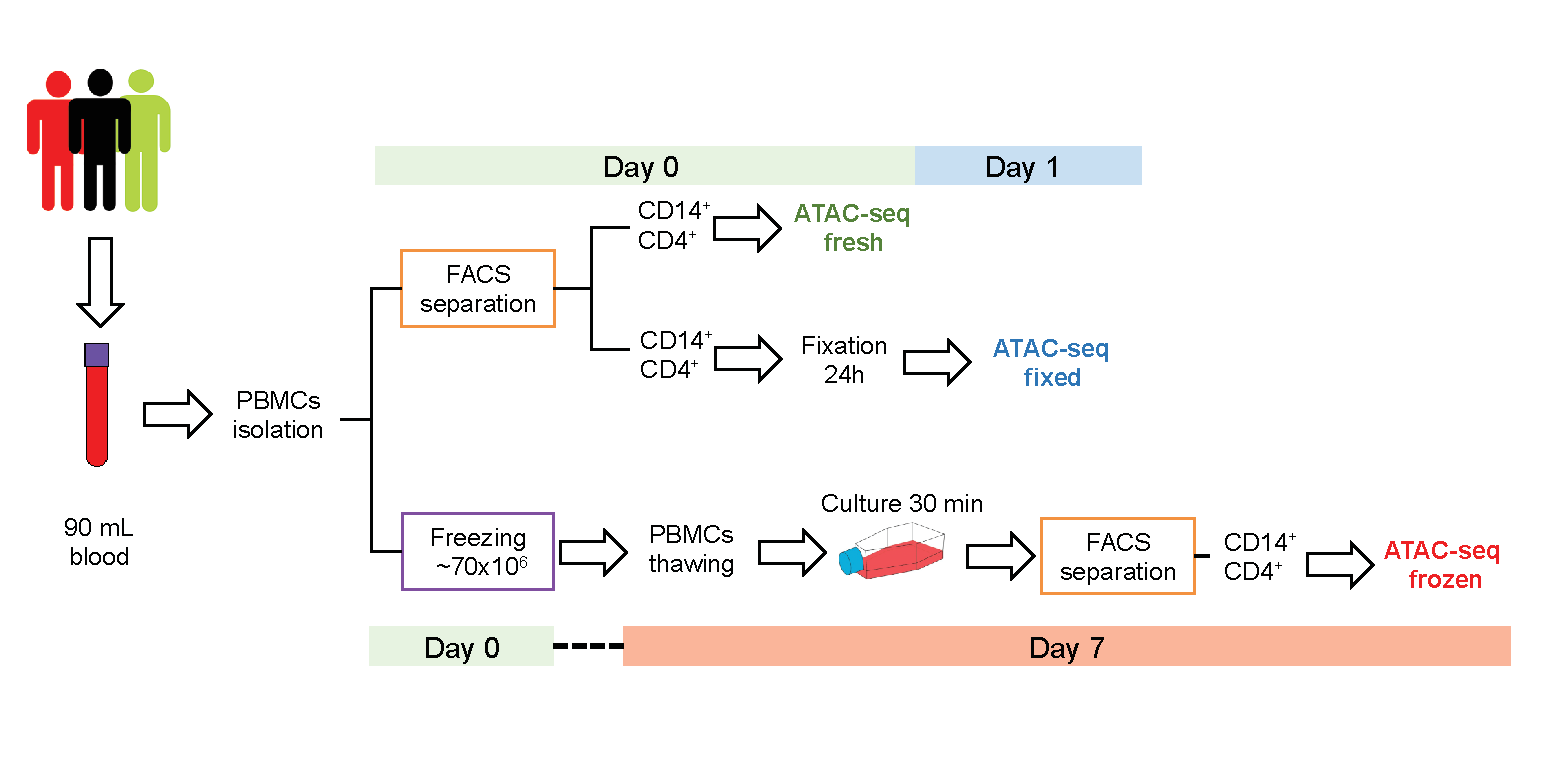
\includegraphics[width=1.2\textwidth]{./Results1/pdfs/Chapter3_core_experimental_design}
\caption[Experimental design to assess the impact of cryopreservation and fixation in the chromatin accessibility of immune primary cells.]{\textbf{Experimental design to assess the impact of cryopreservation and fixation in the chromatin accessibility of immune primary cells.} Three healthy control individuals were recruited on different days, PBMCs were isolated and freshly isolated CD14$^+$ monocytes or CD4$^+$ T cells processed for ATAC-seq immediately (ATAC-seq fresh), after fixation with DPS (ATAC-seq fixed) or after cryopreservation of PBMCs (ATAC-seq frozen).}%Three healthy control individuals were recruited on different days and PBMCs were isolated from 90mL of blood (Day 0). on Day 0, a fraction of PBMCs were used for FACS staining and isolation of 50,000 CD14$^+$ and CD4$^+$, which were directly processed for ATAC-seq (ATAC-seq fresh). Also on Day 0, a 50,000 FACS-sorted CD14$^+$ and CD4$^+$ cells were fixed with DPS, stored at 4{$^\circ$}C for 24h and processed for ATAC-seq in Day 1 (ATAC-seq fixed). Lastly, on Day 0 a fraction of the PBMCs (70x10$^6$ million cells) were cryopreserved in DMSO and slow-cooling. On Day 7 of storage in liquid nitrogen, PBMCs were thawed, recovered in culture for 30 min and stained with FACS Abs to isolate 50,000 CD14$^+$ and CD4$^+$cell to perform ATAC-seq (ATAC-seq frozen).}
\label{figure:Core_experimental_design}
\end{figure}
\end{landscape}

To investigate the effect of cryopreservation and cell recovery in the chromatin landscape of primary immune cells, 70x10$^6$ million PBMCs were cryopreserved with DMSO on the day of collection and stored in liquid nitrogen followed by thawing and recovery in culture for approximately 30 min (as detailed in Chapter \ref{ch:Mat}). After recovery, CD14$^+$ monocytes and CD4$^+$ T cells were isolated from the PBMCs by FACS and then ATAC-seq was performed (Figure \ref{figure:Core_experimental_design} Day 7, ATAC-seq frozen). Altogether, for each volunteer, three matched ATAC-seq libraries were generated in two different cell populations: ATAC-seq fresh, ATAC-seq fixed and ATAC-seq frozen.

\subsubsection{Assessment of the chromatin structure preservation in the different conditions}

All samples from each of the two cell types had more than 15 million reads, which has previously been shown as the minimum for successful ATAC-seq analysis and peak calling (Figure \ref{figure:Core_ATAC_all_conditions_total_reads}). The median number of reads across the fresh, frozen and fixed were more similar for CD14$^+$ monocytes (58.6, 64.2 and 39.6 million reads, respectively) than in the CD4$^+$ samples, where the frozen and fixed presented lower median total reads compared to the controls (43.8, 32.9 and 28.8 million reads respectively) (Figure \ref{figure:Core_ATAC_all_conditions_total_reads}A and B).

\begin{figure}[htbp]
\centering
\begin{subfigure}{0.5\textwidth}
\centering
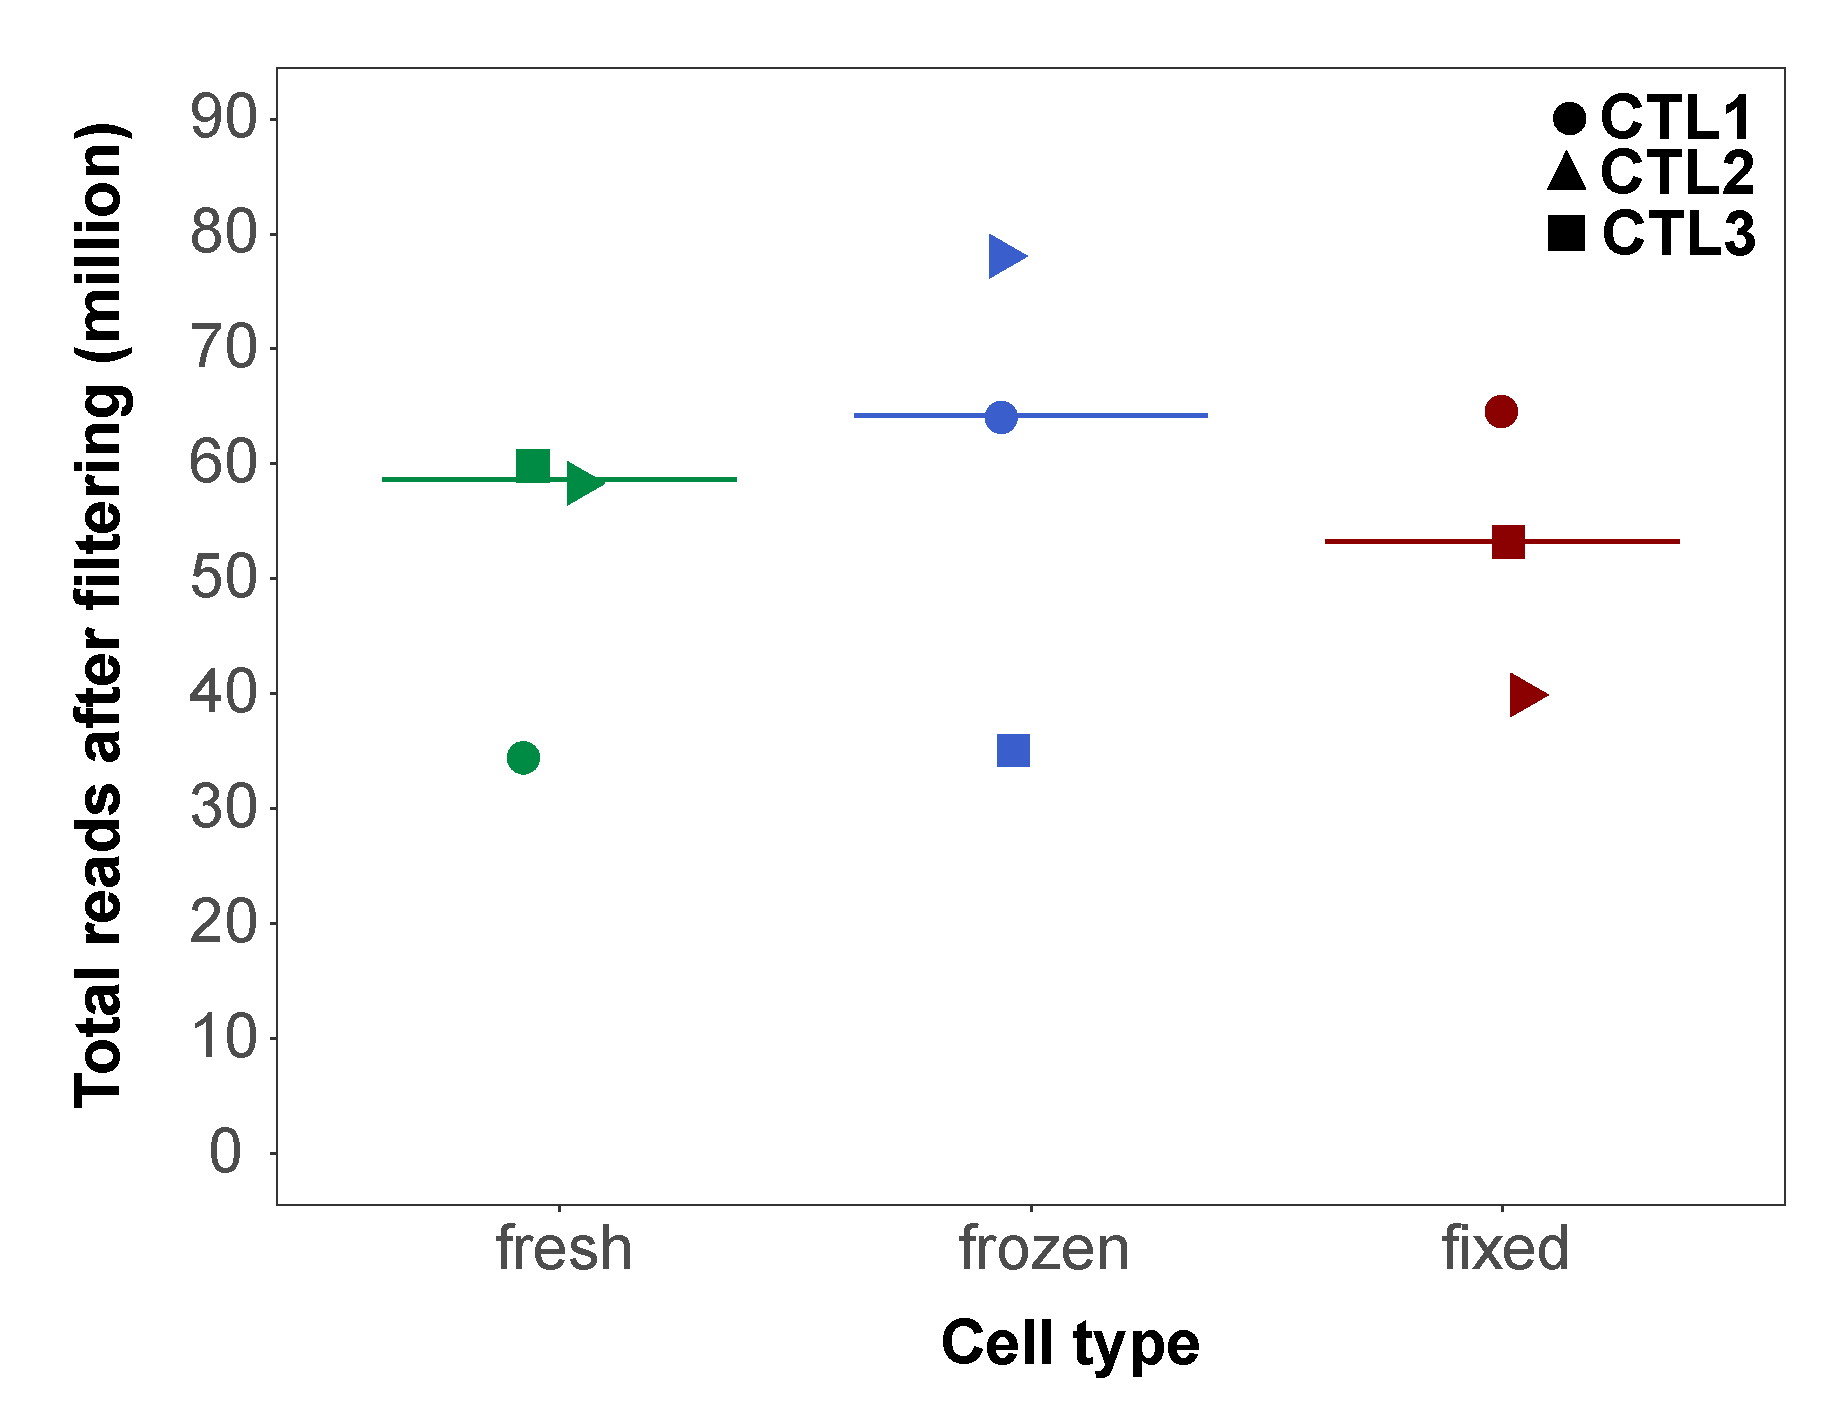
\includegraphics[width=\textwidth]{./Results1/pdfs/Core_ATAC_CD14_fresh_frozen_fixed_filtered_total_reads}
\caption{\textbf{}}
% The percentage sign indicated that the other subfig goes side by side
\end{subfigure}%
\begin{subfigure}{0.5\textwidth}
\centering
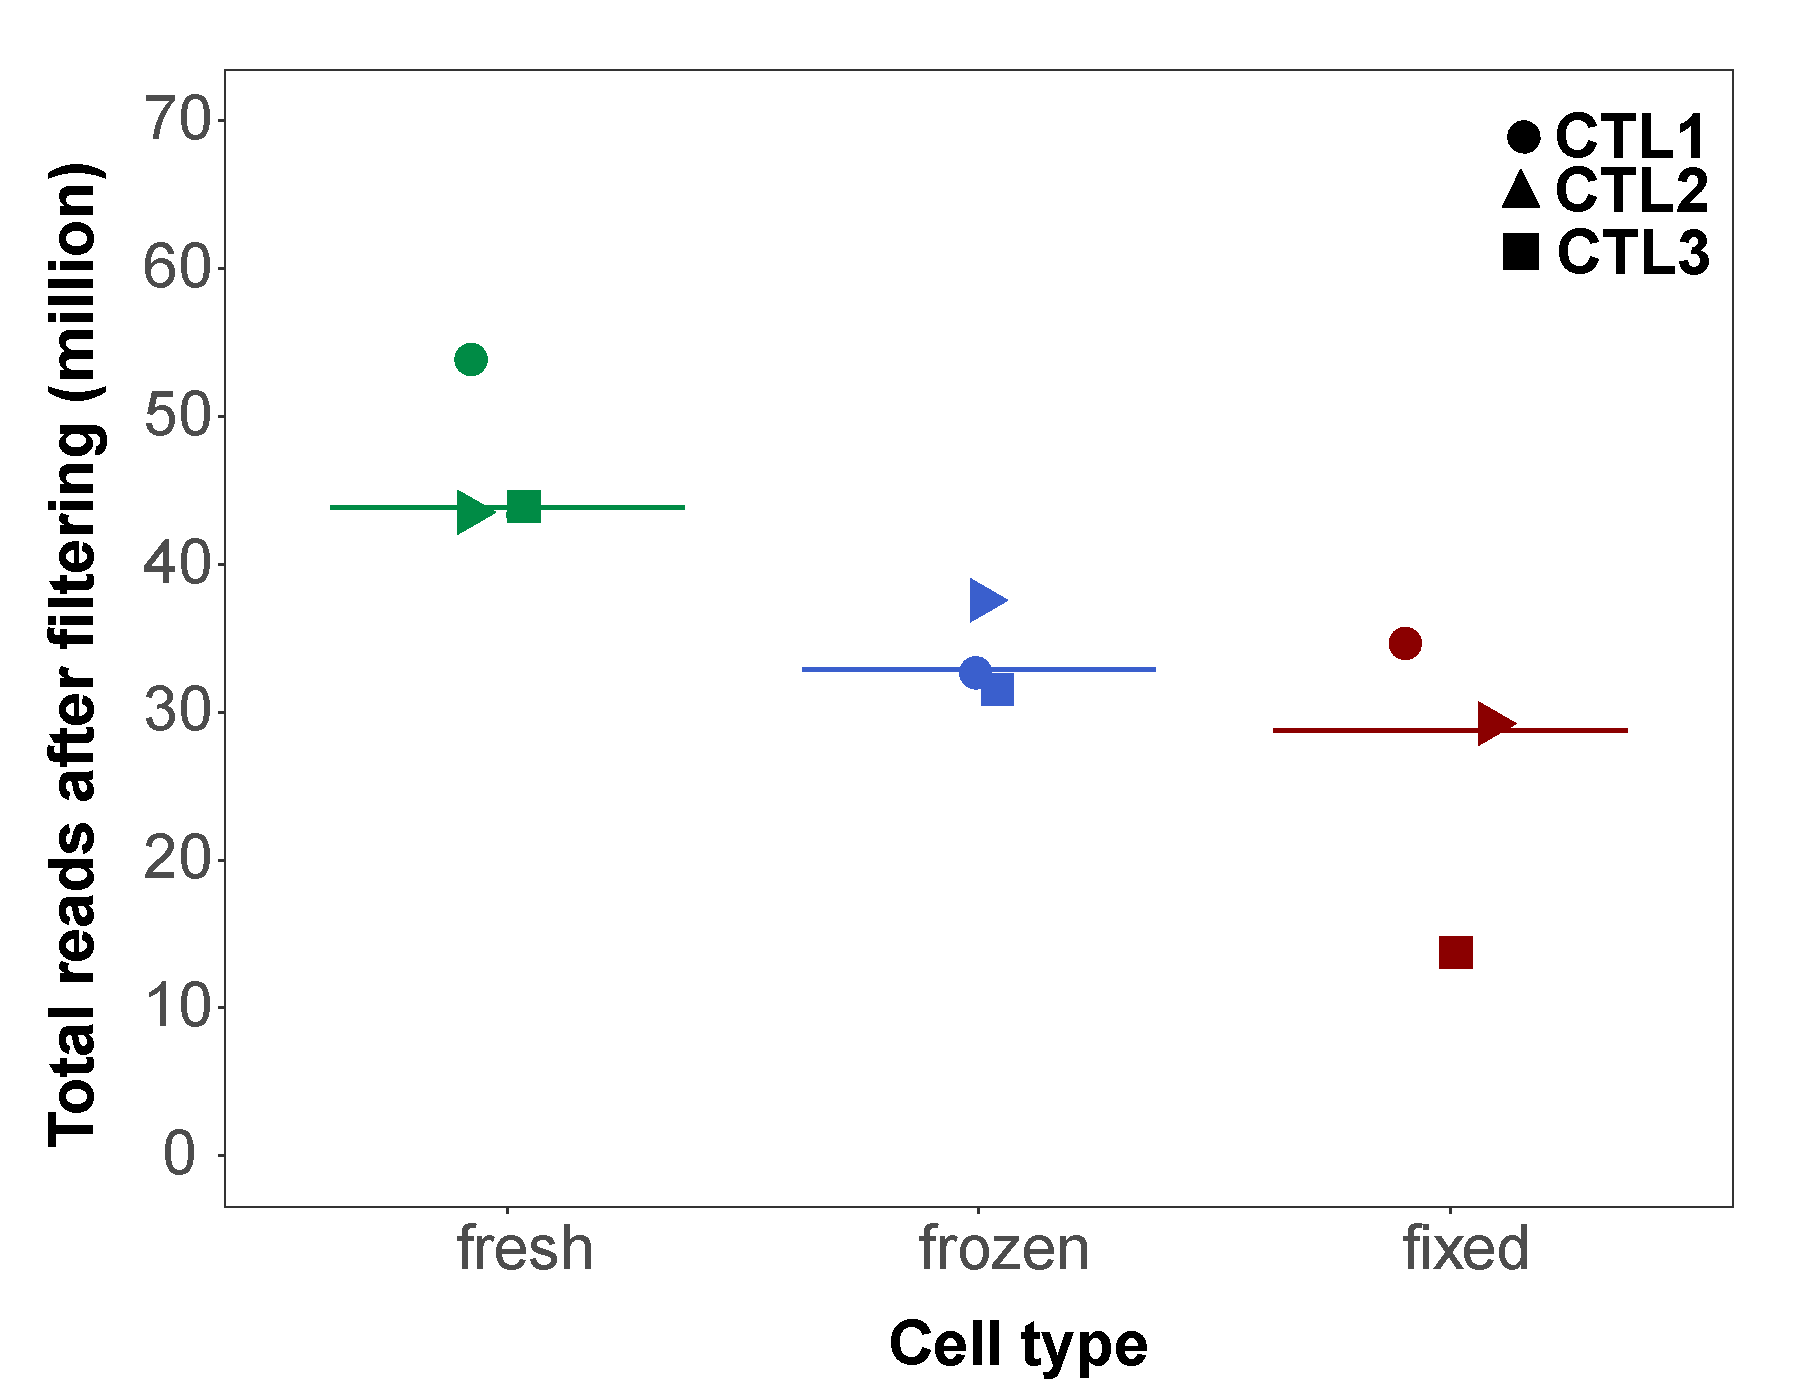
\includegraphics[width=\textwidth]{./Results1/pdfs/Core_ATAC_CD4_fresh_frozen_fixed_filtered_total_reads}
\caption{\textbf{}}
\end{subfigure}
\caption[Total number of ATAC-seq reads for the fresh, frozen and fixed CD14$^+$ monocytes and CD4$^+$ samples for three volunteers (CTL1-3).]{\textbf{Total number of ATAC-seq reads for the fresh, frozen and fixed CD14$^+$ monocytes and CD4$^+$ samples for three volunteers (CTL1-3).} Representation of million reads after filtering for the fresh, fixed and frozen ATAC-seq libraries in (A) CD14$^+$ monocytes and (B) CD4$^+$ cells.}
\label{figure:Core_ATAC_all_conditions_total_reads}
\end{figure} 

The ATAC-seq signal-to-noise ratios across the TSS showed a similar median for the fresh and fixed CD14$^+$ monocytes libraries (17.4 and 16.5 fold-enrichment, respectively) and was higher for the frozen samples (26.3 fold-enrichment)(Table \ref{tab:Core_ATAC_TSS_summary_table}). The median TSS enrichments in the frozen and fixed CD4$^+$ samples were considerably higher (16.1 and 14.3 fold-enrichment, respectively) than the fresh samples (5.6), which were borderline for the ENCODE recommended threshold. For one volunteer (CTL1) the fixed samples of both cell types showed considerably lower TSS enrichment (2.5 and 7.9, respectively) compared to the other fixed samples (Table \ref{tab:Core_ATAC_TSS_summary_table}). As expected, the fragment size distribution profiles of the fresh and frozen samples for both cell types were very similar, showing appropriate relative abundance of NFF and NBF corresponding to mono-, di-, tri- and tetra-nucleosomes (Figure \ref{figure:Core_ATAC_all_fragment_size_distribution}A and B green and blue lines). Conversely, fixed samples showed differences in the fragment size distribution profiles, where for both cell types a fraction of NFF was absent in CTL1 and lower than NBF in CTL2 and CTL3 (Figure \ref{figure:Core_ATAC_all_fragment_size_distribution} red lines). 


Chromatin structure across and within the TSS was then investigated following Scharer and colleagues approach \parencite{Scharer2016}. The nucleosome-free fragments ($<$150bp) from all the samples showed a single peak of enrichment at the nucleosome-depleted TSS position, with CD4$^+$ fresh samples presenting the lowest relative enrichment (Figure \ref{figure:Core_ATAC_intra_dinucleosome_tss_enrichment}A and C).

\begin{figure}[htbp]
\centering
\begin{subfigure}{0.5\textwidth}
\centering
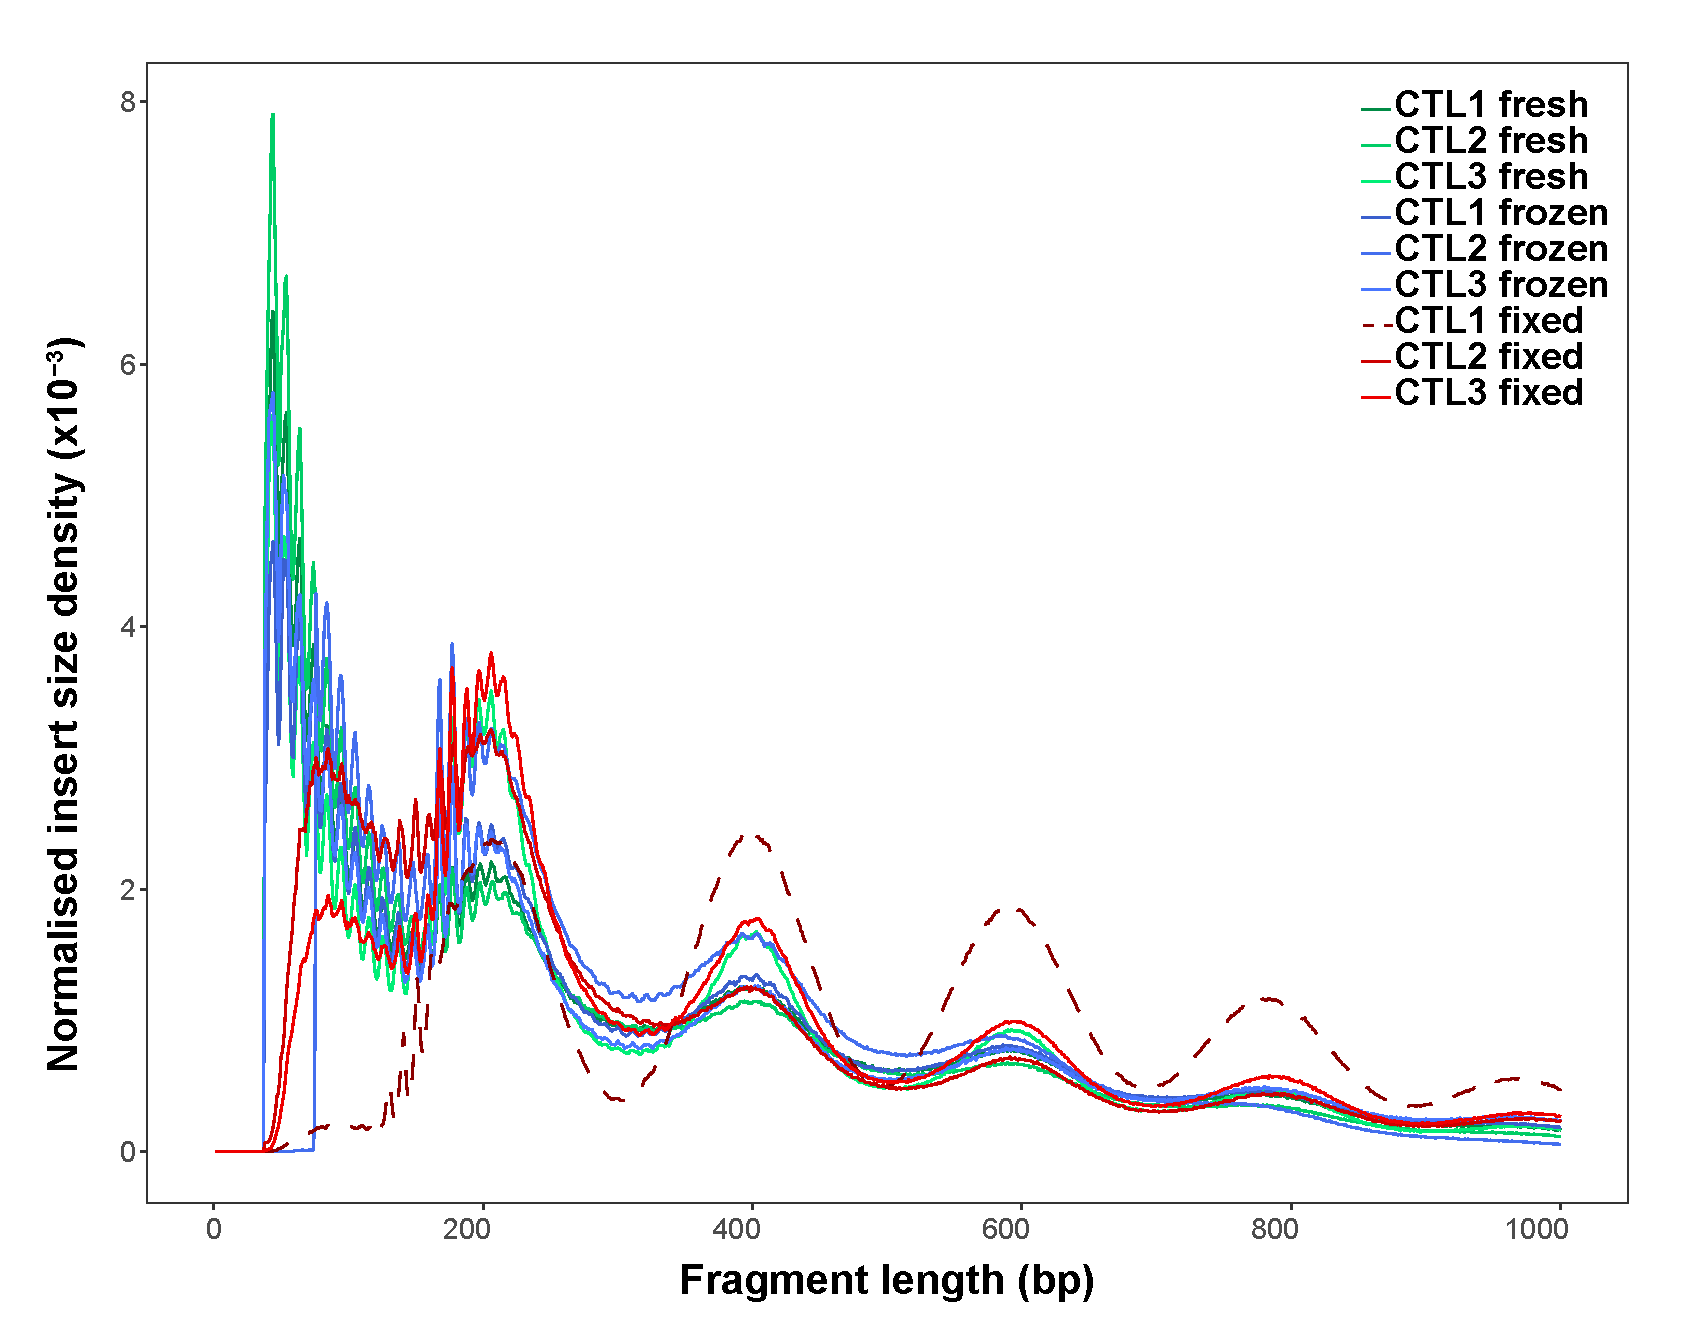
\includegraphics[width=\textwidth]{./Results1/pdfs/Core_ATAC_CD14_fresh_frozen_fixed_frag_size_distribution}
\caption{\textbf{}}
% The percentage sign indicated that the other subfig goes side by side
\end{subfigure}%
\begin{subfigure}{0.5\textwidth}
\centering
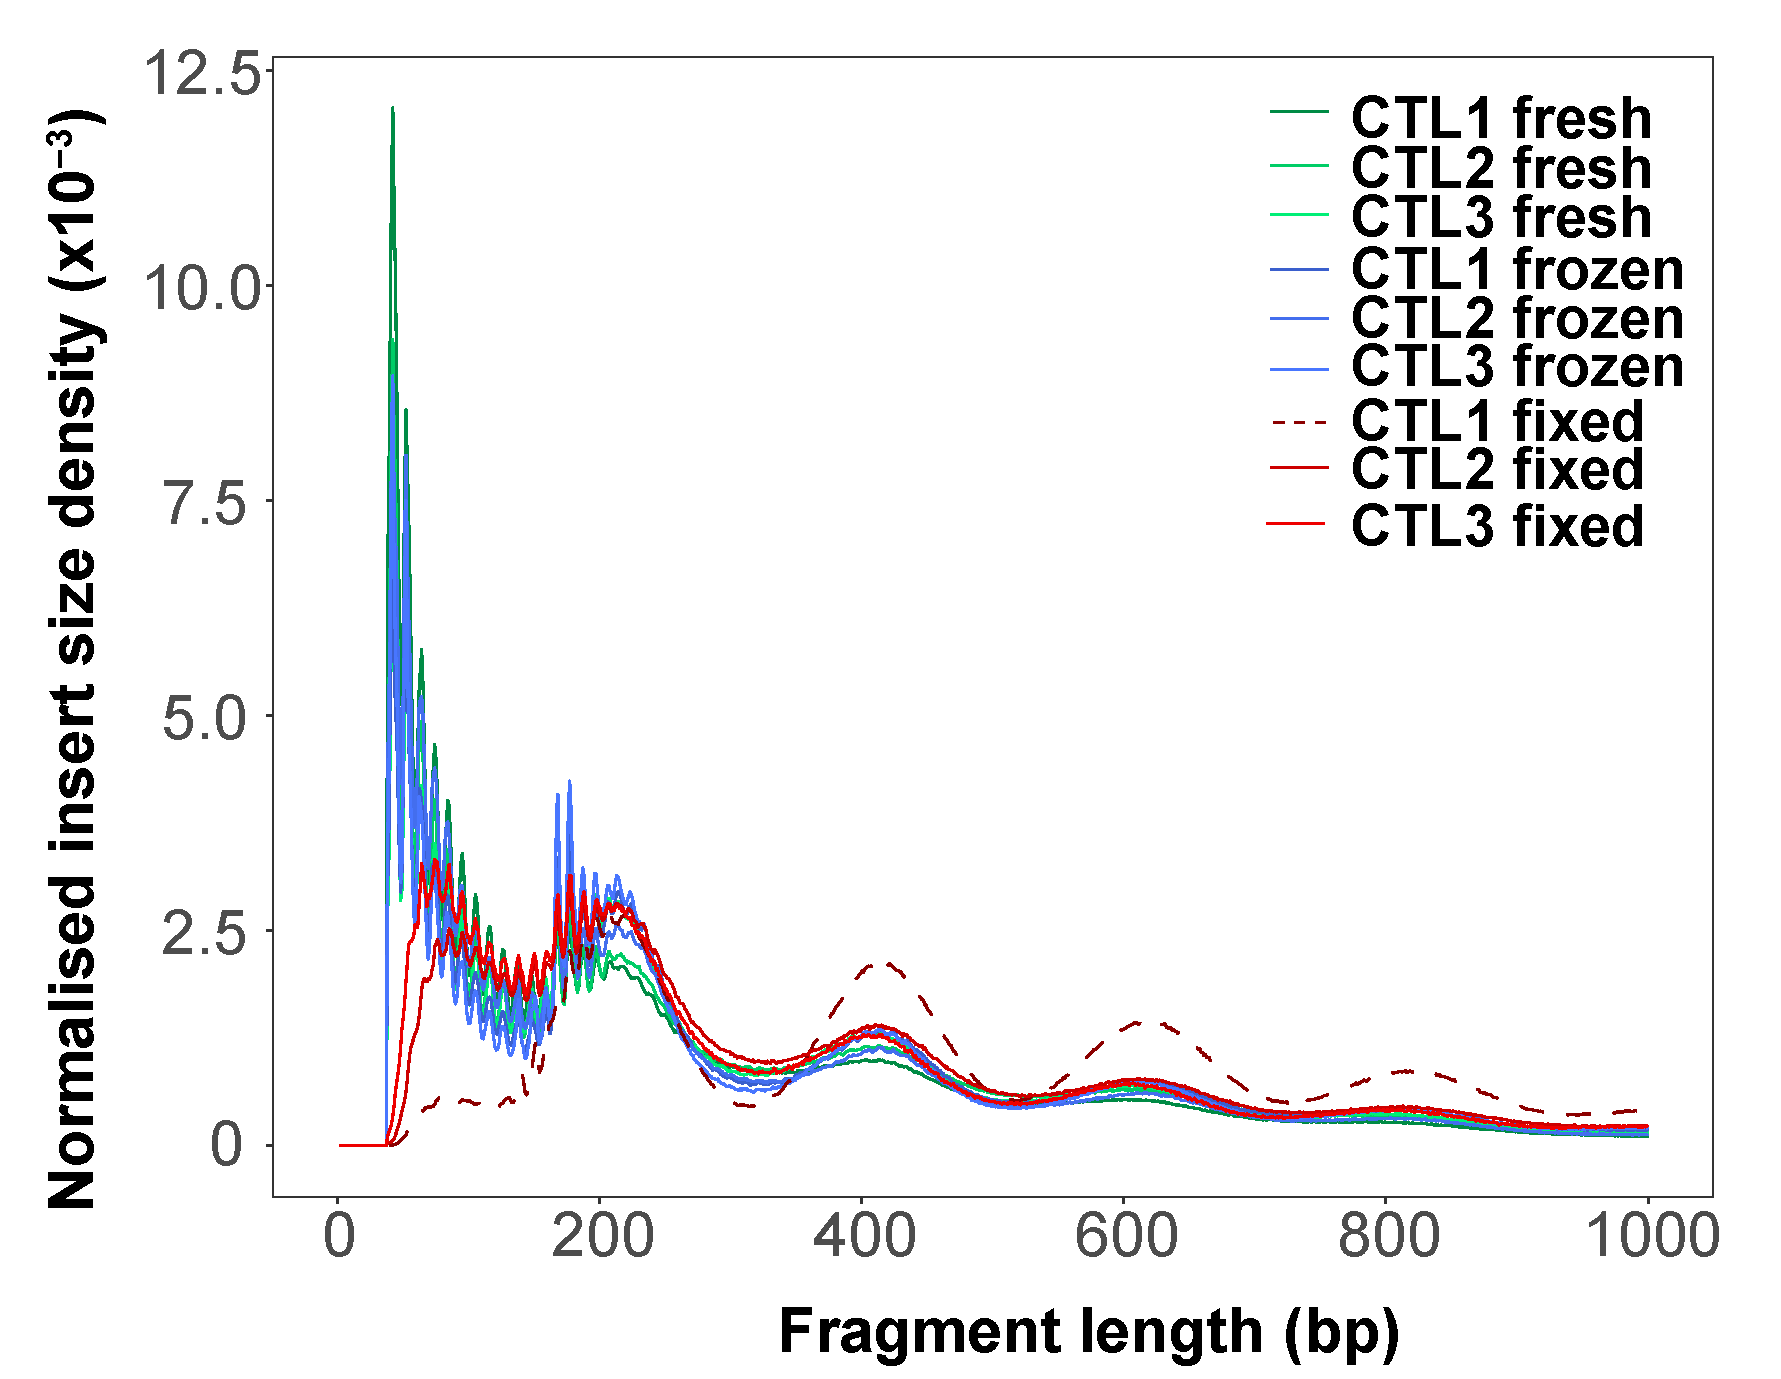
\includegraphics[width=\textwidth]{./Results1/pdfs/Core_ATAC_CD4_fresh_frozen_fixed_frag_size_distribution}
\caption{\textbf{}}
\end{subfigure}
\caption[Fragment size density distribution for ATAC-seq fresh, fixed and frozen in CD14$^+$ monocytes and CD4$^+$ cells.]{\textbf{Fragment size density distribution for ATAC-seq fresh, fixed and frozen in CD14$^+$ monocytes and CD4$^+$ cells.} The distribution of ATAC-seq fragment lengths are illustrated for (A) CD14$^+$ monocytes and (B) CD4$^+$ cells and colour-coded by condition (fresh=green, frozen=blue and fixed=red).}
\label{figure:Core_ATAC_all_fragment_size_distribution}
\end{figure} 


The pattern of enrichment of di-nucleosome fragments (ranging between 260 and 340bp) demonstrated in the majority of the samples periodicity in the TSS surroundings, with two peaks of enrichment mapping at the characteristic up-stream and down-stream positioned nucleosomes (Figure \ref{figure:Core_ATAC_intra_dinucleosome_tss_enrichment}B and D). Although fixation in CD14$^+$ and CD4$^+$ CTL1 samples drastically reduced the abundance of NFF, the ATAC-seq signal for the remaining ones was clearly enriched at TSS (Figure \ref{figure:Core_ATAC_intra_dinucleosome_tss_enrichment}A and C). Interestingly, despite fixed CD14$^+$ CTL1 having increased density of NBF (in this case di-, tri- and tetra-nucleosomes) loss of chromatin structure around the TSS suggested that nucleosomes may have been displaced from their original position, likely due to the fixative not cross-linking proteins to DNA, and therefore explaining this lack of enrichment (Figure \ref{figure:Core_ATAC_intra_dinucleosome_tss_enrichment}B). CD4$^+$ fresh samples showed comparatively low enrichment at the TSS for NFF and di-nucleosome fragments, consistent with the overall borderline signal-to-noise ratio of the samples (Figure \ref{figure:Core_ATAC_intra_dinucleosome_tss_enrichment}B and D and Table \ref{tab:Core_ATAC_TSS_summary_table}).


%This pattern of enrichment was weaker in the three fresh samples from CD4$^+$ and absent in the CTL1 CD14$^+$ fixed sample. The fresh CD4$^+$ samples also presented low enrichment for the nucleosome-free fragments in the TSS, similar to their overall TSS enrichment (Table \ref{tab:Core_ATAC_TSS_summary_table}) but still weakly identified the position of the two nucleosomes in the TSS surroundings, suggesting an overall preservation of the chromatin structure. 



\begin{figure}[htbp]
\centering
\begin{subfigure}[b]{0.45\textwidth}
\centering 
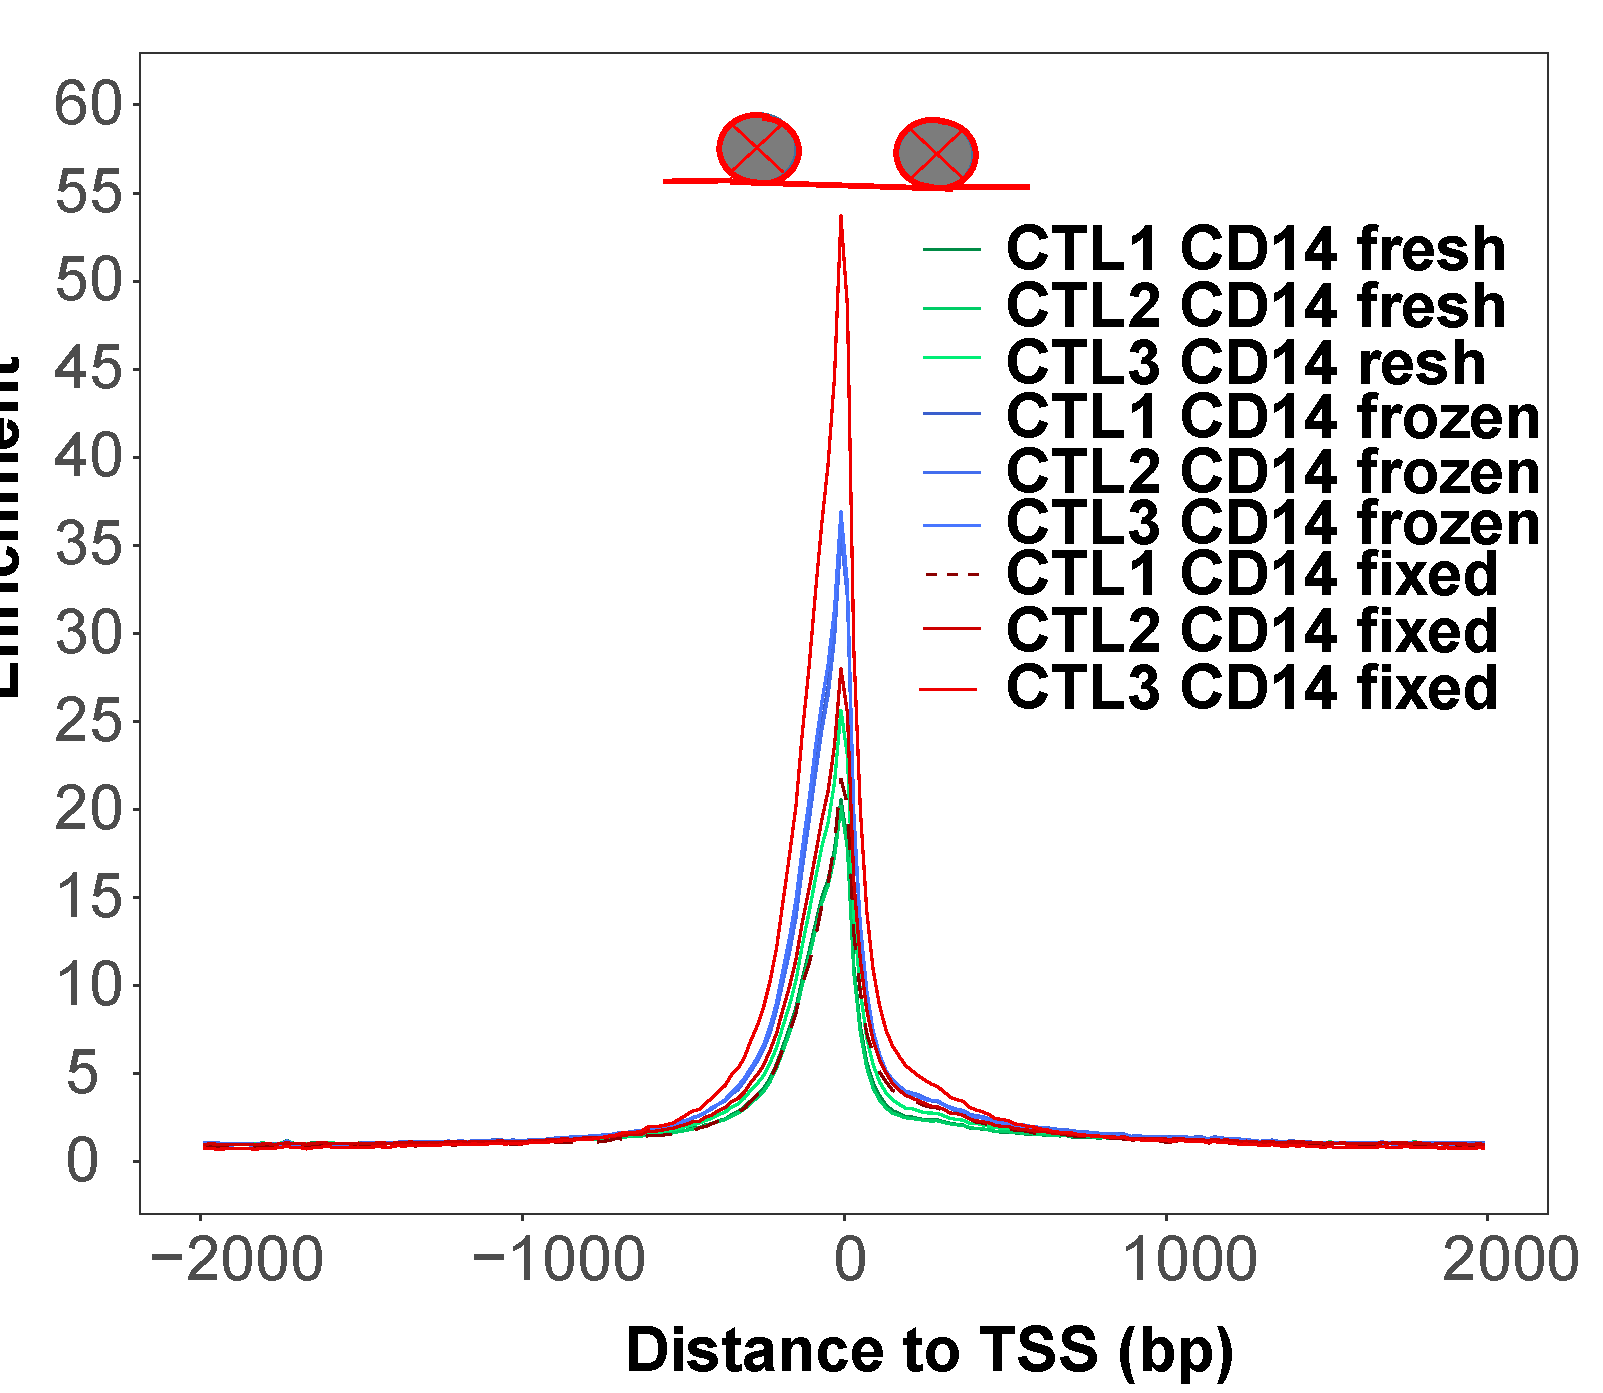
\includegraphics[width=\textwidth]{./Results1/pdfs/Core_ATAC_CD14_fresh_frozen_fixed_internucleosome_TSS}
\caption{}
\end{subfigure}
~
\begin{subfigure}[b]{0.45\textwidth}
\centering 
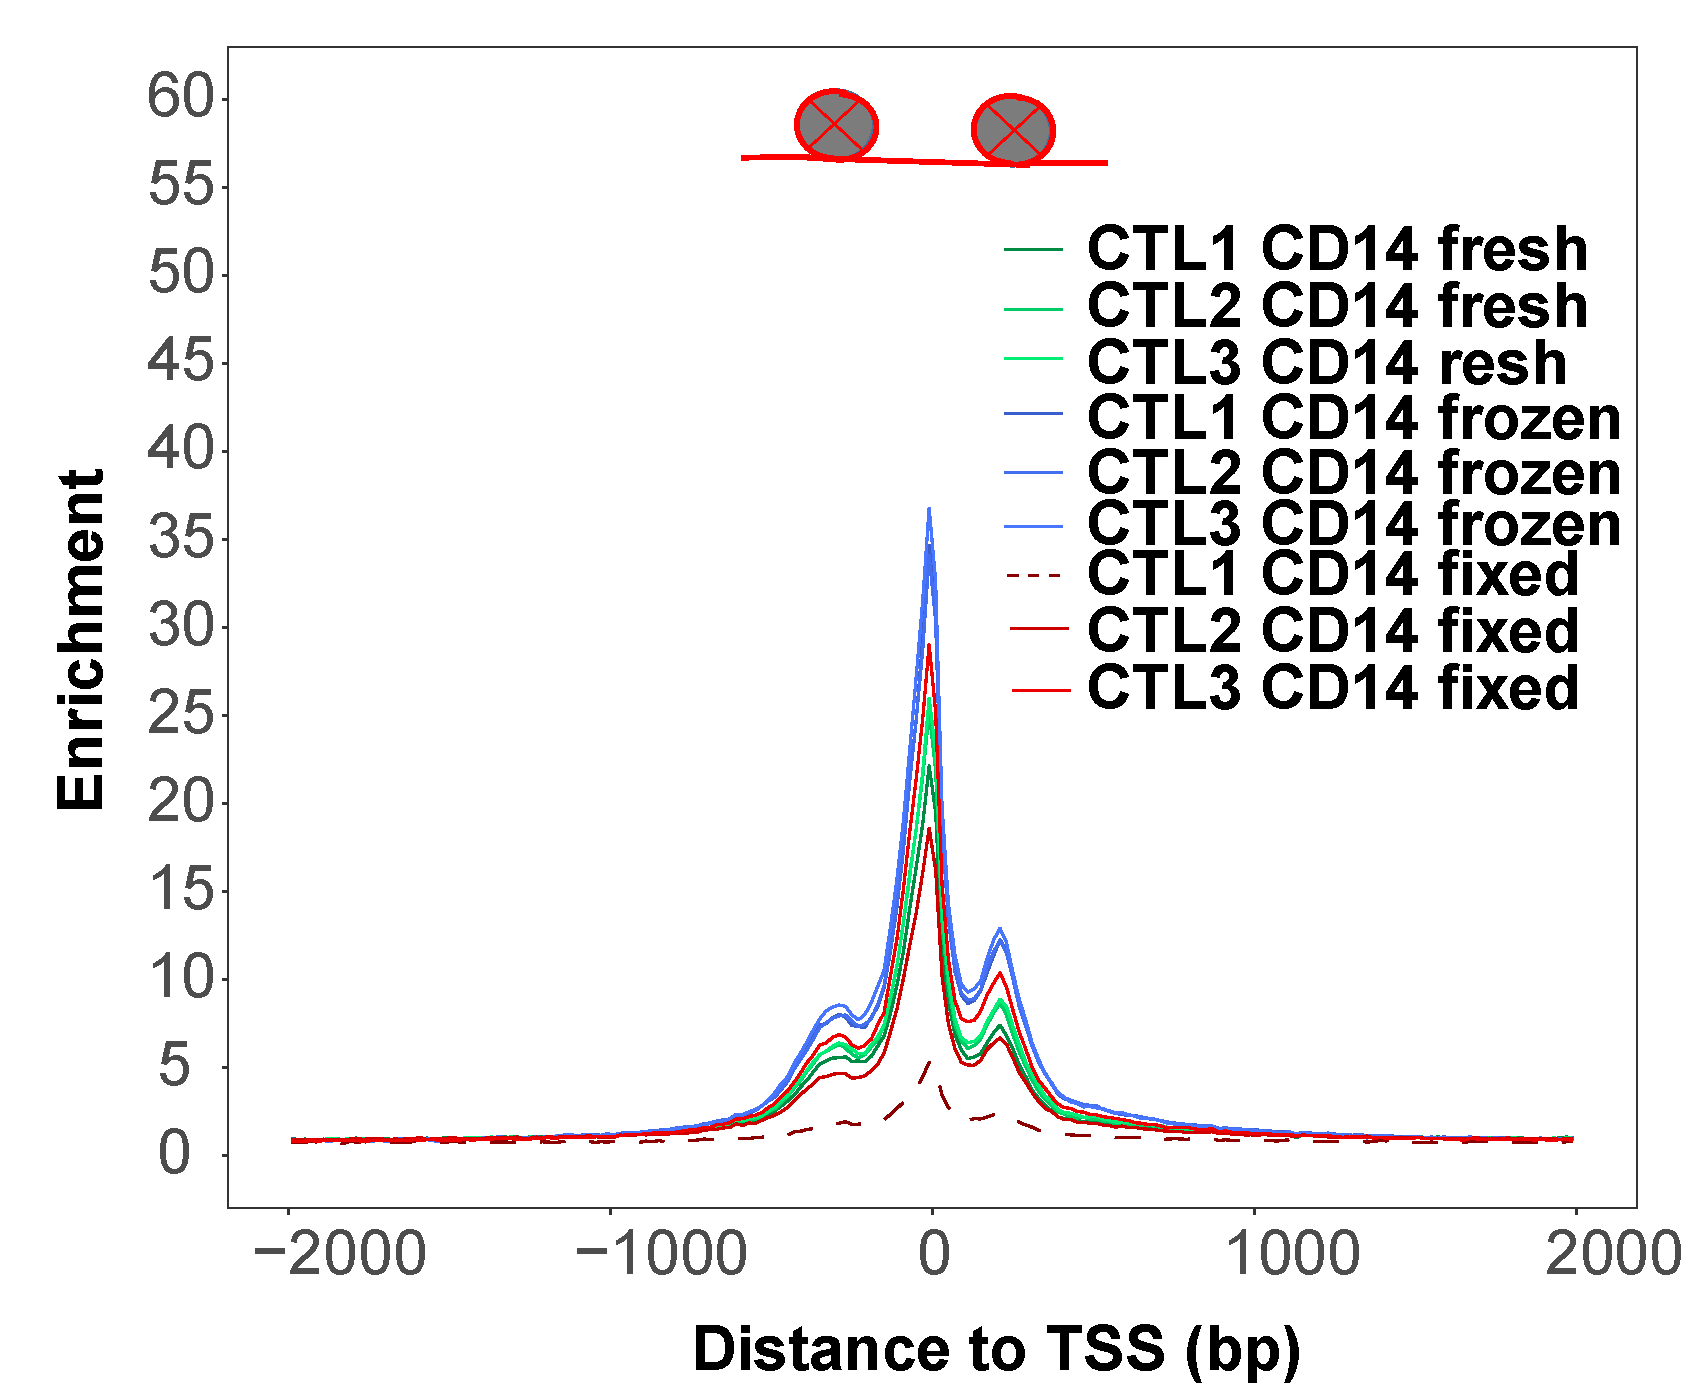
\includegraphics[width=\textwidth]{./Results1/pdfs/Core_ATAC_CD14_fresh_frozen_fixed_dinucleosome_TSS}
\caption{}
\end{subfigure}
~
\begin{subfigure}[b]{0.45\textwidth} 
%the [b] prevents offset in subcaptions
\centering
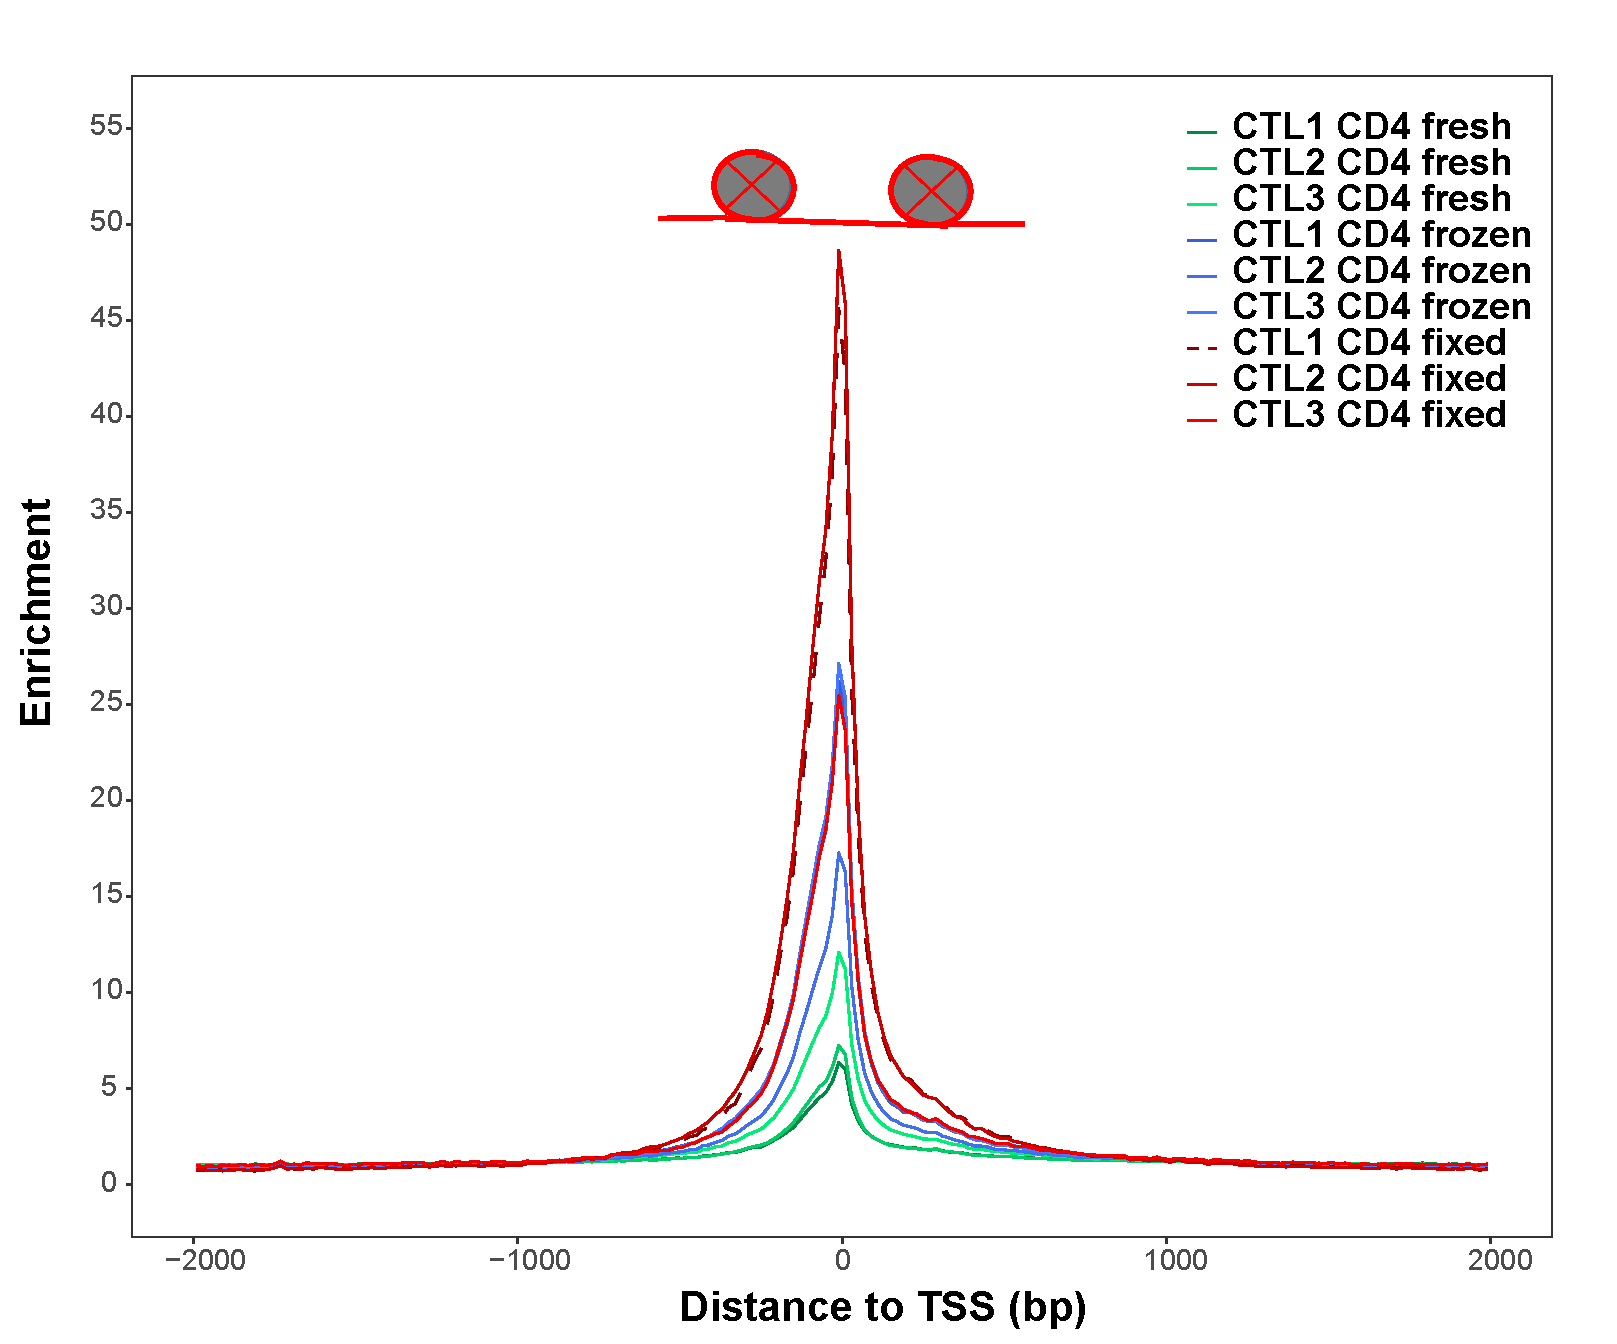
\includegraphics[width=\textwidth]{./Results1/pdfs/Core_ATAC_CD4_fresh_frozen_fixed_internucleosome_TSS}%
\caption{}
\end{subfigure}
\begin{subfigure}[b]{0.45\textwidth} 
%the [b] prevents offset in subcaptions
\centering
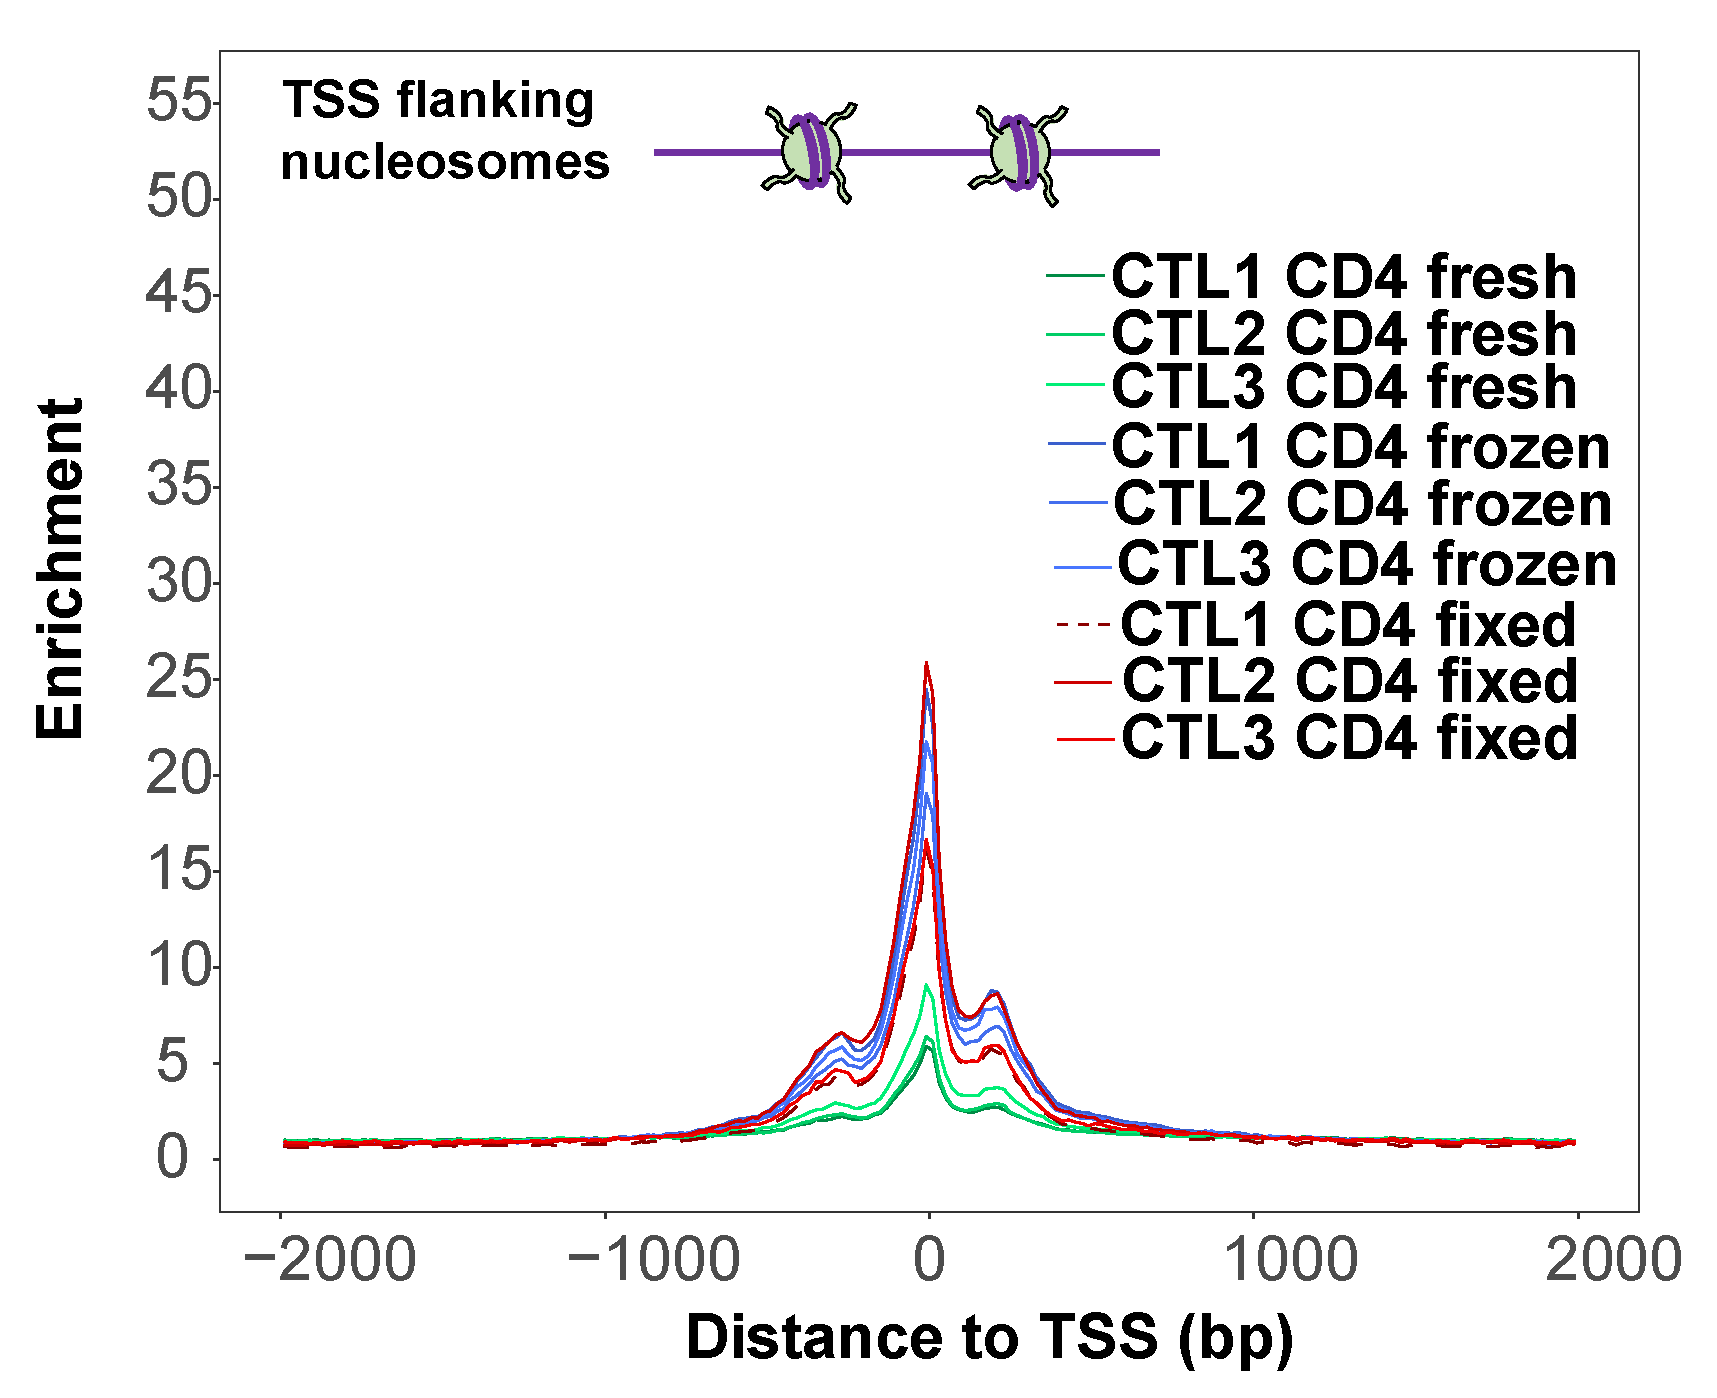
\includegraphics[width=\textwidth]{./Results1/pdfs/Core_ATAC_CD4_fresh_frozen_fixed_dinucleosome_TSS}%
\caption{}
\end{subfigure}
\caption[ATAC-seq enrichment of nucleosome-free and di-nucleosome fragments at the TSS and surroundings in CD14$^+$ monocytes and CD4$^+$ samples for the three conditions.]{\textbf{ATAC-seq enrichment of nucleosome-free and di-nucleosome fragments at the TSS and surroundings in CD14$^+$ monocytes and CD4$^+$ samples for the three conditions.} For each of the samples, nucleosome-free fragments ($<$150bp) or di-nucleosome (between 260 and 340bp) fragments were selected \textit{in silico}. Enrichment at $+/-$1Kb across all the Ensembl annotated TSS is shown for (A) CD14$^+$ monocytes or (C) CD4$^+$ T cells nucleosome-free fragments and for (B) CD14$^+$ monocytes and (D) CD4$^+$ T cells di-nucleosome fragments. The two nucleosomes flanking the TSS are depicted at the top of each graph.}
\label{figure:Core_ATAC_intra_dinucleosome_tss_enrichment}
\end{figure}



Annotation of the significant peaks identified in each sample (filtered using the IDR strategy as explained in \ref{peak_filtering}) revealed that the highest proportion of ATAC-seq peaks localised to promoters, introns and intergenic regions (Figure \ref{figure:Core_ATAC_all_conditions_genomic_features}A and B), consistent with previous studies \parencite{Buenrostro2013,Scharer2016}. Interestingly, the ATAC-seq libraries showing higher percentage of peaks at promoter regions corresponded to fixed samples, in which chromatin structure was incompletely preserved, and to fresh CD4$^+$ T cells, with borderline signal-to-noise ratios based on TSS enrichment analysis. The higher percentage of peaks annotated as promoters in in low quality samples revealed reduced ability of these samples to capture genomic features with more moderate chromatin accessibility and bias for the the location of significant robust peaks at the most stable and distinctive open chromatin sites in the genome.

Overall, this analysis demonstrated that the chromatin structure from DSP fixed ATAC-seq libraries was not fully preserved in either of the two cell types, as they all showed a distinct pattern of fragment size distribution in comparison to fresh and frozen samples, as well as loss of nucleosome positioning across the TSS only in CTL1 fixed samples. 

\begin{figure}[htbp]
\centering
\begin{subfigure}{0.5\textwidth}
\centering
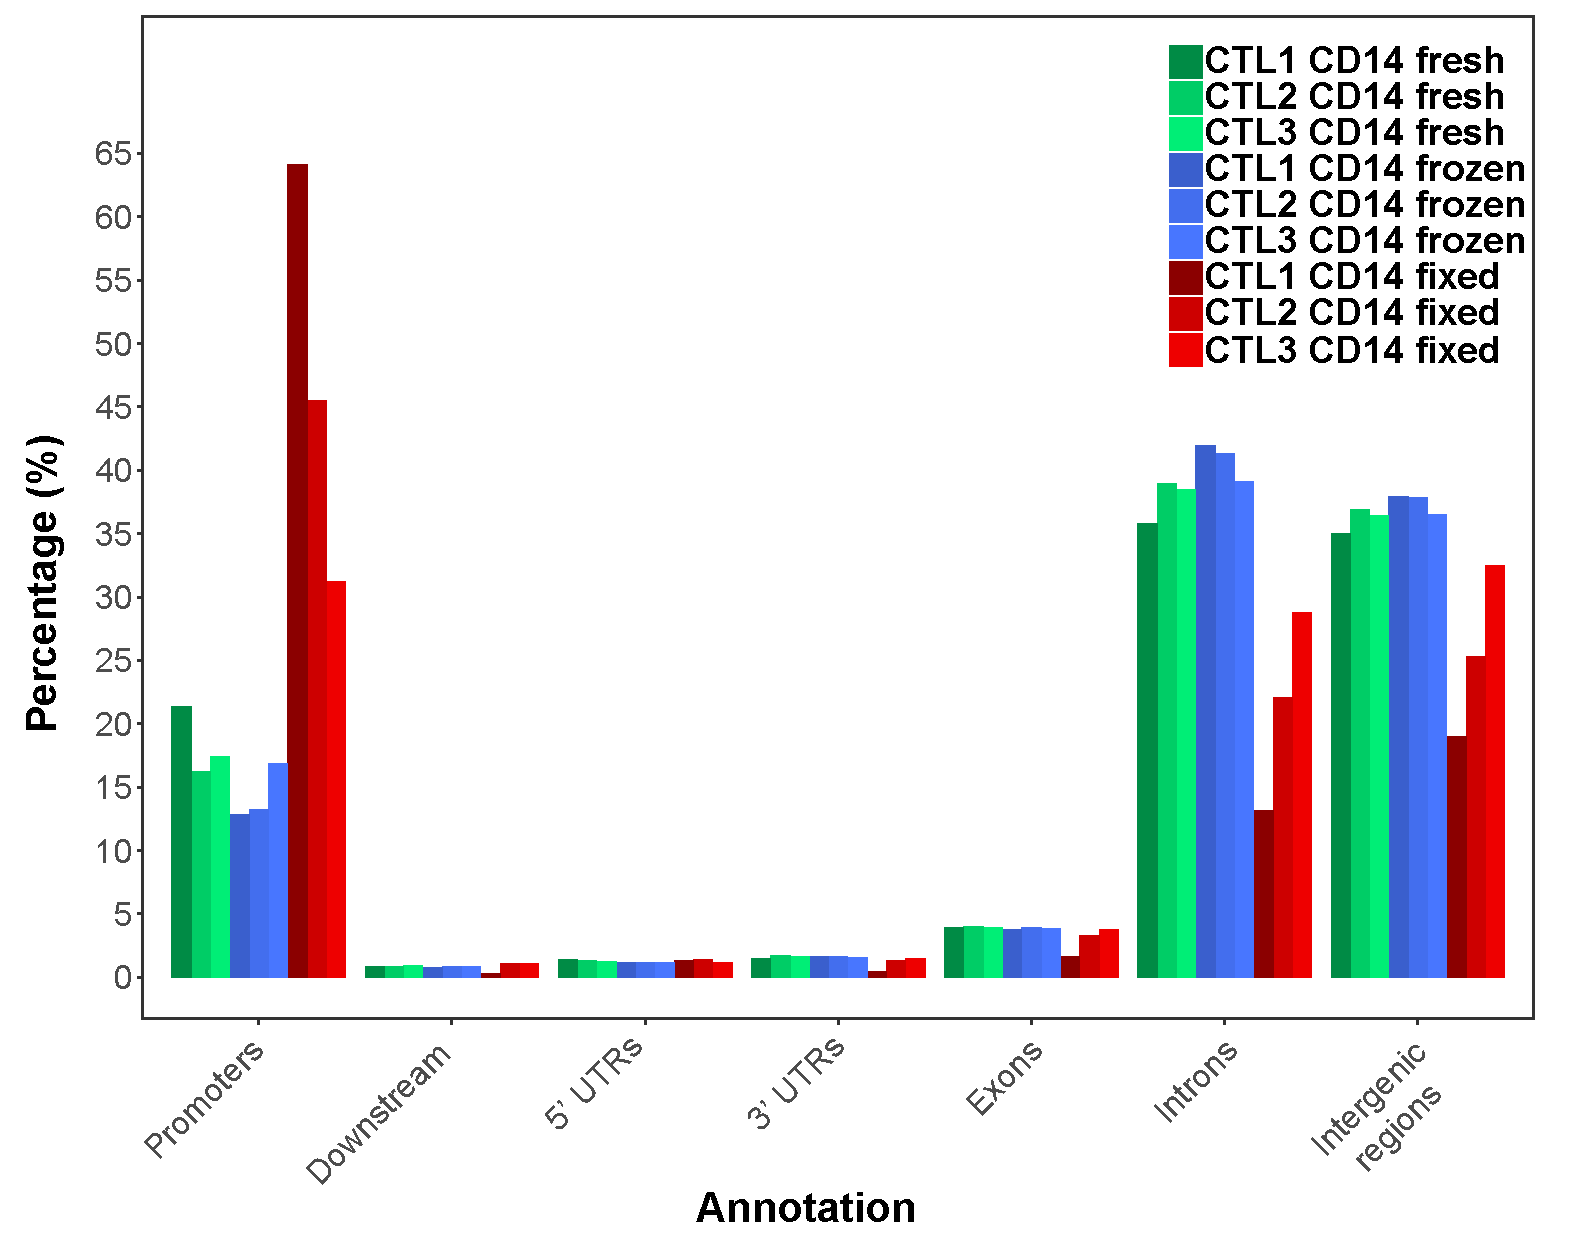
\includegraphics[width=\textwidth]{./Results1/pdfs/Core_ATAC_CD14_fresh_frozen_fixed_IDR_filtered_peak_annotation}
\caption{\textbf{}}
% The percentage sign indicated that the other subfig goes side by side
\end{subfigure}%
\begin{subfigure}{0.5\textwidth}
\centering
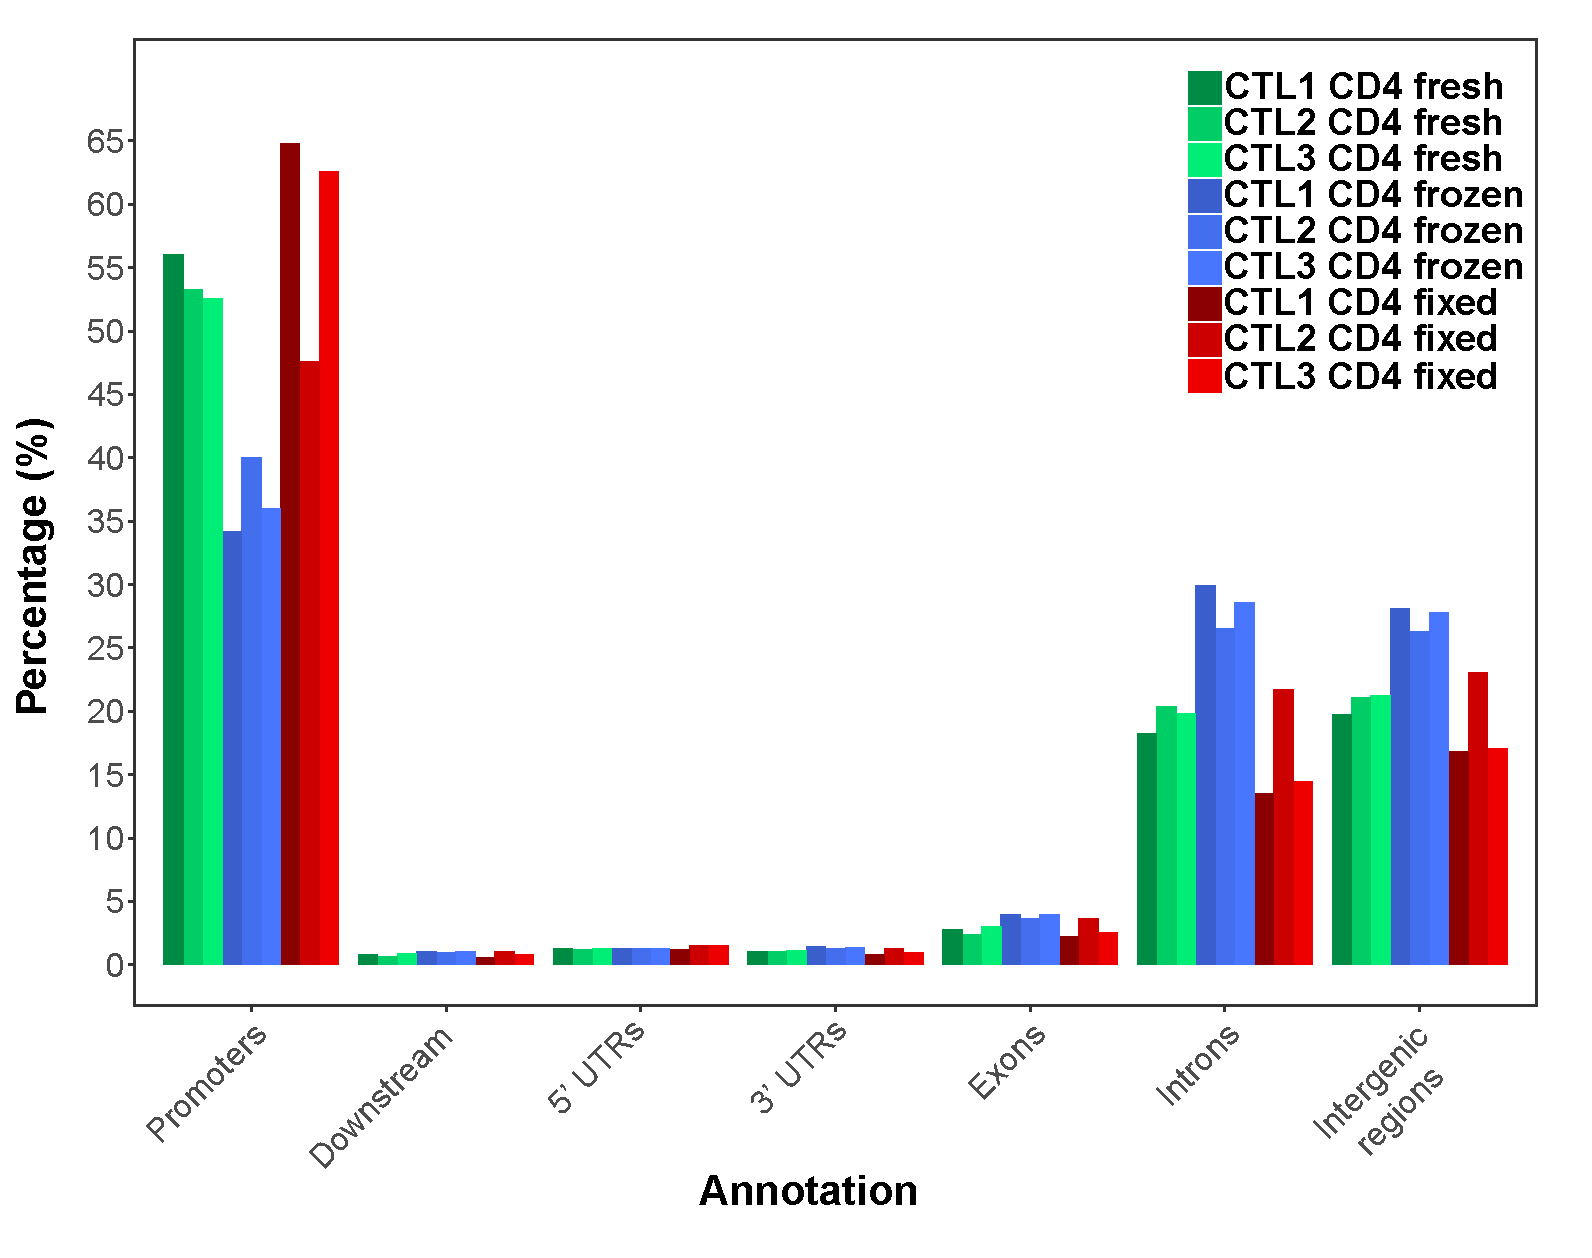
\includegraphics[width=\textwidth]{./Results1/pdfs/Core_ATAC_CD4_fresh_frozen_fixed_IDR_filtered_peak_annotation}
\caption{\textbf{}}
\end{subfigure}
\caption[Genomic features annotation for the ATAC-seq peaks called in each of the fresh, frozen and fixed samples from CD14$^+$ monocytes and total CD4$^+$.]{\textbf{Genomic features annotation for the ATAC-seq peaks called in each of the fresh, frozen and fixed samples from CD14$^+$ monocytes and CD4$^+$.} Overlap was performed between the genomic features and the list of (A) CD14$^+$ monocytes and (B) CD4$^+$ peaks, filtered for the corresponding optimal p-value based on the pseudoreplicates IDR analysis in each sample and condition (fresh=green, frozen=blue and fixed=red).}
\label{figure:Core_ATAC_all_conditions_genomic_features}
\end{figure} 


Lastly, principal component analysis (PCA) was conducted separately in CD14$^+$ monocytes and CD4$^+$ T cells using the normalised counts retrieved at each of the ATAC peaks from the consensus list built including samples from the three conditions (CP\_CD14\_all\_cond and CP\_CD4\_all\_cond, respectively), with the exception of fixed CTL1 (considerably different from the other two fixed samples). Plotting the first two principal components (PCs) showed sample clustering based on condition in both cell types and demonstrated that the largest source of variability correlated with the way samples were processed (Figure \ref{figure:Core_ATAC_all_conditions_PCA}). 



\begin{figure}[htbp]
\centering
\begin{subfigure}{0.5\textwidth}
\centering
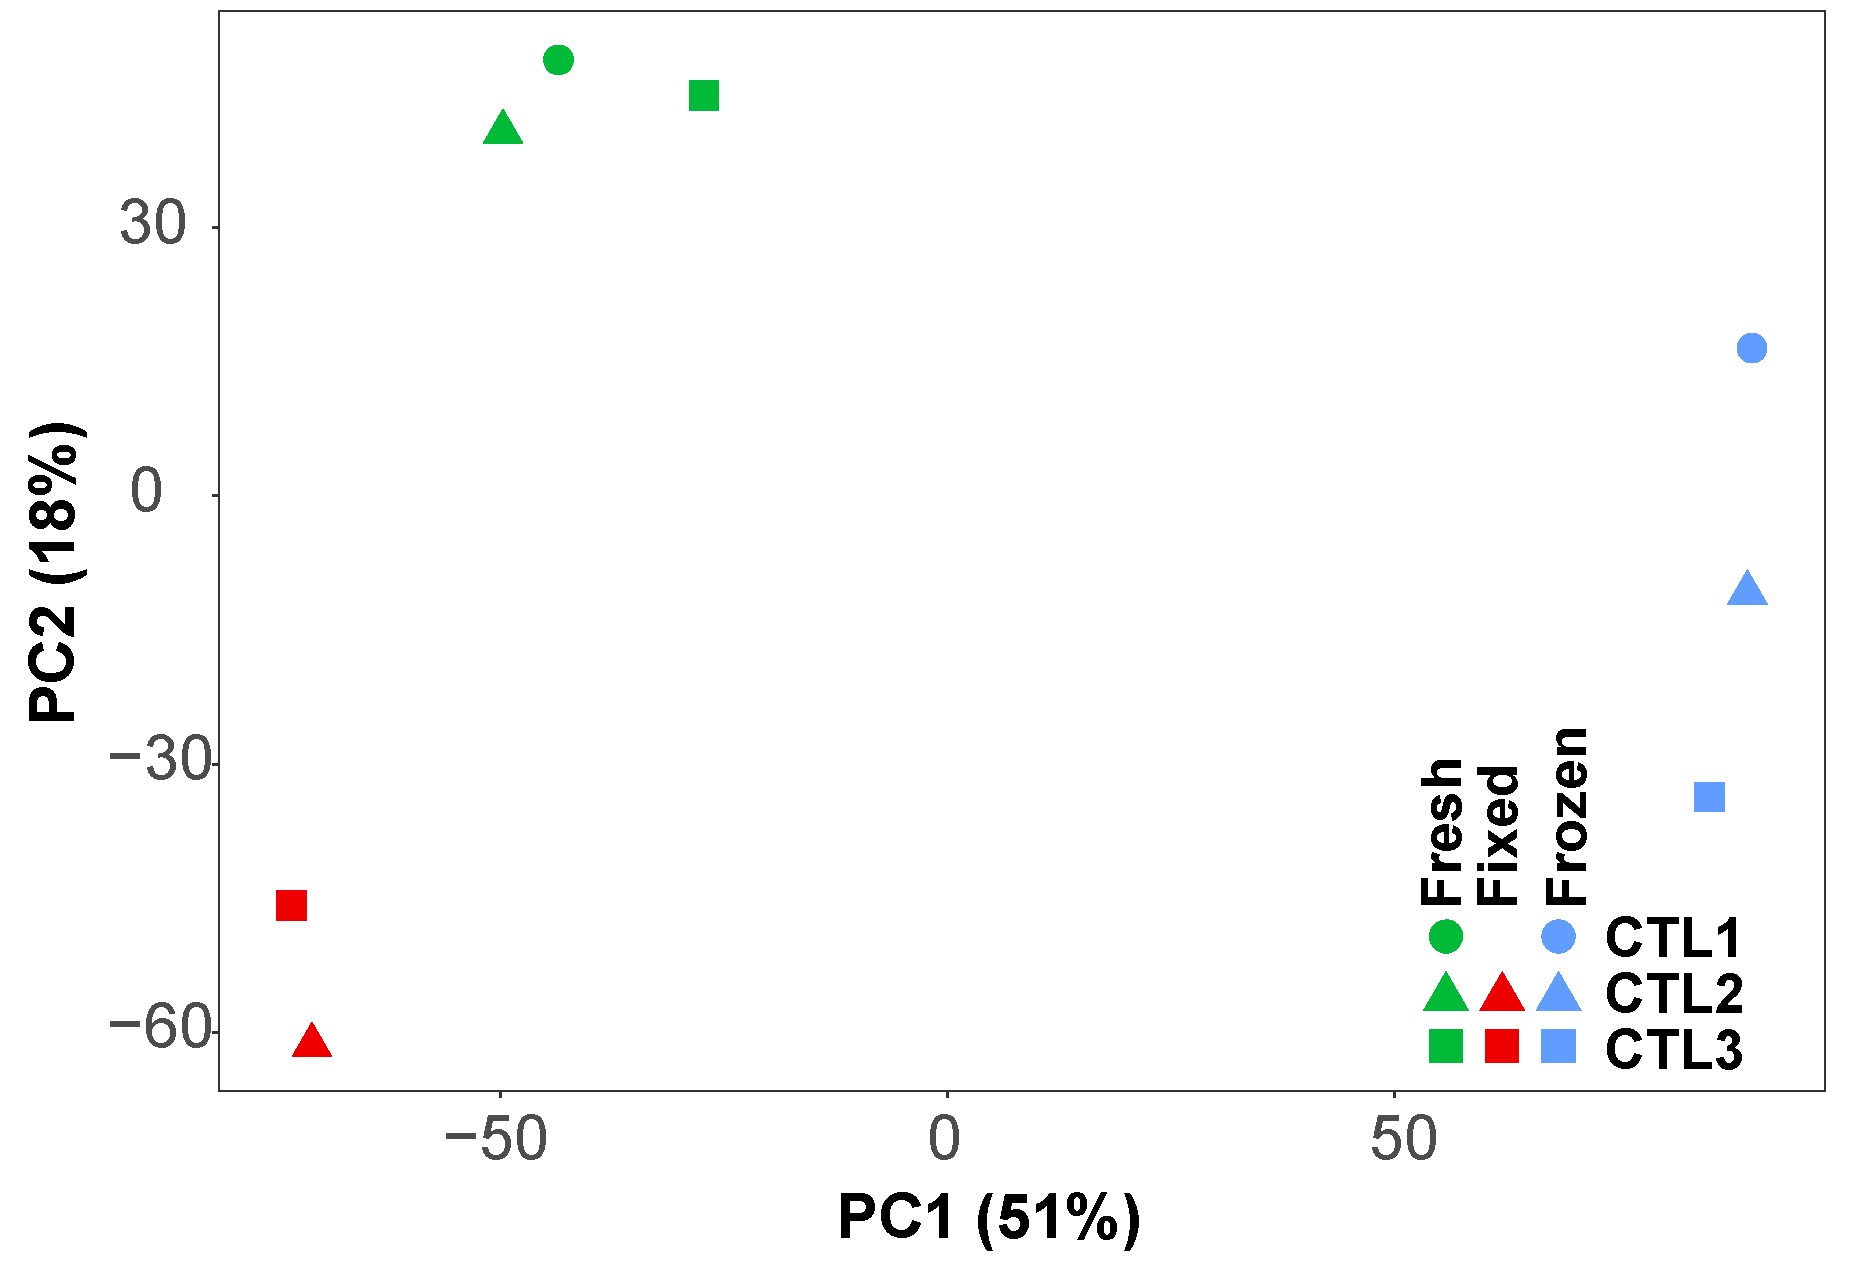
\includegraphics[width=\textwidth]{./Results1/pdfs/Core_ATAC_CD14_fresh_frozen_fixed_no_CTL1_fixed_PCA}
\caption{\textbf{}}
% The percentage sign indicated that the other subfig goes side by side
\end{subfigure}%
\begin{subfigure}{0.5\textwidth}
\centering
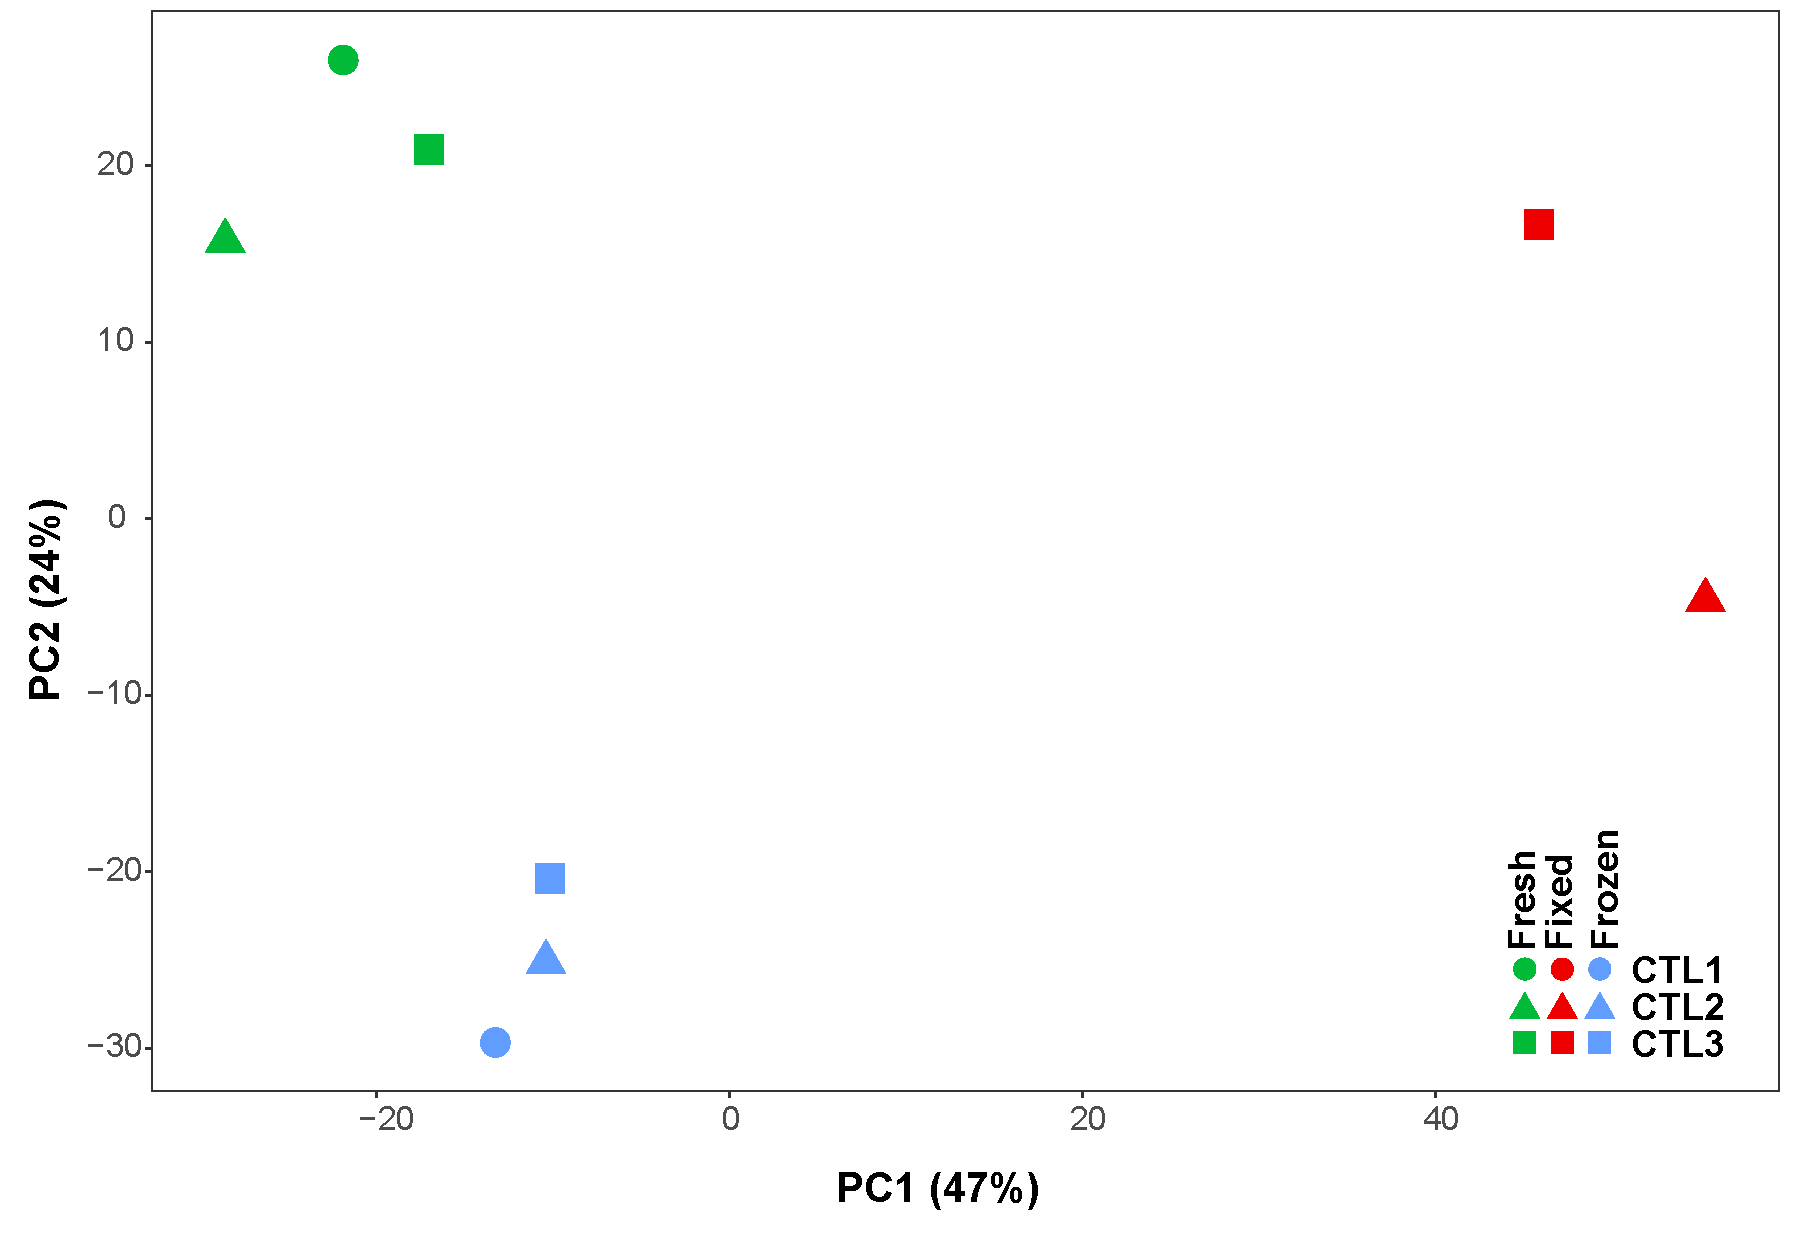
\includegraphics[width=\textwidth]{./Results1/pdfs/Core_ATAC_CD4_fresh_frozen_fixed_no_CTL1_fixed_PCA}
\caption{\textbf{}}
\end{subfigure}
\caption[PCA based on the ATAC-seq chromatin accessibility landscape in fresh, fixed and frozen samples.]{\textbf{PCA based on the ATAC-seq chromatin accessibility landscape in fresh, fixed and frozen samples.} PCA was performed using the normalised counts across the consensus list of ATAC peaks from the combined fresh, fixed and frozen samples (CP\_CD14\_all\_cond and CP\_CD4\_all\_cond) in (A) CD14$^+$ monocytes or (B) CD4$^+$ cells from the same three healthy individuals. The first two PCs (x-axis and y-axis, respectively) of all the regions included in each of the consensus peak list are plotted. Each point represents a sample, where shape codes for individual (CTL1, CTL2, CTL3) and colour means condition (fresh, fixed, frozen). The proportion of variation explained by each principal component is indicated in brackets.}
\label{figure:Core_ATAC_all_conditions_PCA}
\end{figure}




\subsubsection{Differential chromatin accessibility analysis between fresh and frozen samples}

In order to determine the effect of the freezing and recovery process in the chromatin landscape of CD14$^+$ monocytes and CD4$^+$ T cells, genome-wide differences between ATAC-seq fresh (biological reference) and frozen were investigated. Since the use of DSP as a fixative was already found to impact preservation of the chromatin structure, differential analysis between fresh and fixed samples was not conducted as the results may be confounded. Comparison between ATAC-seq fresh and ATAC-seq frozen within each cell types was performed using the normalised read counts for the list of ATAC peaks included in the consensus list. Overall, ATAC-seq normalised counts showed high correlation between fresh and frozen samples in the two cell types, with the lowest correlation (R=0.918) found in CD14$^+$ monocytes (Figure \ref{figure:Core_ATAC_all-conditions_correlation}A, B).


\begin{figure}[H]
\centering
\begin{subfigure}[b]{0.45\textwidth}
\centering 
\includegraphics[width=\textwidth]{./Results1/pdfs/Core_ATAC_CD14_fresh_frozen_correlation_counts_small_new}
\caption{}
\end{subfigure}
~
\begin{subfigure}[b]{0.45\textwidth}
\centering 
\includegraphics[width=\textwidth]{./Results1/pdfs/Core_ATAC_CD4_fresh_frozen_correlation_counts_small_new}
\caption{}
\end{subfigure}
\caption[Comparison of the log$_2$ normalised ATAC-seq counts at the consensus list of peaks in fresh and frozen conditions.]{\textbf{Comparison of the log$_2$ normalised ATAC-seq counts at the consensus consensus list of peaks in fresh, fixed and frozen conditions.} Each plot shows the comparison of ATAC-seq log$_2$ mean normalised counts from the CP\_CD14\_all\_cond or CP\_CD4\_all\_cond filtered for background noise (80\% empirical cut-off) between fresh and frozen (A) CD14$^+$ monocytes and (B) CD4$^+$ T cells. Pearson correlation coefficient (R) is indicated.}
\label{figure:Core_ATAC_all-conditions_correlation}
\end{figure}
	


The differential chromatin accessibility analysis between ATAC-seq fresh and frozen samples using DEseq2 revealed a total of 5,123 and 177 significant DARs (FDR$<$0.01 and fold change$>$1.5) and a larger proportion of regions (12.6 and 1.3\%) changing chromatin accessibility between fresh and frozen samples in CD14$^+$ monocytes compared to CD4$^+$ T cells, respectively. Nevertheless, the percentage of sites identified as DARs in relation to the total number of investigated regions for both cell types suggested only moderate changes in the chromatin accessibility landscape between fresh and frozen conditions. 


%To further assess the differences in chromatin accessibility, differential chromatin accessibility analysis between ATAC-seq fresh and ATAC-seq fixed or frozen at each of the ML\_CD14\_all\_cond and ML\_CD14\_all\_cond peaks was performed using DESeq2. The number of significant DARs (FDR$<$0.01) reported for in each of the comparisons mirrored the PCA analysis results (Table \ref{tab:Core_ATAC_all_conditions_DARs}). In CD14$^+$ monocytes, the largest number of DARs (5,269) was reported when comparing ATAC-seq frozen to the fresh reference state. Conversely, in CD4$^+$ the greatest differences in chromatin accessibility were found between fresh and fixed ATAC-seq samples (1,564 DARs).  	
	
	
\begin{table}[htbp]
%\setlength{\tabcolsep}{20pt} only to stretch the columns if you want
%\renewcommand{\arraystretch}{1.5}
\centering
\begin{tabular}{@{} c c c}
\toprule
\textbf{Cell type} & \textbf{Total regions in} & \textbf{DARs} \\
                   & \textbf{consensus list}   & \textbf{(percentage)} \\
\midrule
\midrule
CD14$^+$ monocytes & 40,600                    & 5,123 (12.6\%) \\
CD4$^+$            & 13,025                    & 177  (1.3\%) \\
\bottomrule
\end{tabular}
\medskip %gap
\caption[Summary results from the differential chromatin accessibility analysis comparing ATAC-seq frozen or fixed chromatin landscape to the reference ATAC-seq fresh.]{\textbf{Summary results from the differential chromatin accessibility analysis comparing ATAC-seq frozen or fixed chromatin landscape to the reference ATAC-seq fresh.} The number of regions in the consensus list (CP\_CD14\_all\_cond or CP\_CD4\_all\_cond) following filtering for background counts using 80\% cut-off and the number of significant DARs (FDR$<$0.01 and fold change$>$1.5) are shown. In brackets, the percentage of DARs over the total number of regions included in the differential analysis is indicated.}
\label{tab:Core_ATAC_all_conditions_DARs}
\end{table}
\bigskip %bigger space


In order to identify biological processes that may altered by the changes in chromatin accessibility between conditions, enrichment analysis was conducted using as input the genes proximal ($\leq$5Kb) to the significant DARs (FDR$<$0.01 and fold change$>$1.5) identified in each cell type. Significantly enriched Gene Ontology (GO) biological processes (FDR$<$0.01) were only identified for proximal genes to DARs in CD14$^+$ (Figure \ref{figure:Core_CD14_fresh_vs_frozen_GOBP_barplot}). This included changes in chromatin accessibility of regions in proximity to genes involved in cell shape and cell adhesion, lipopolysaccharide-mediated signalling, inflammation and signal transduction, amongst others, suggesting that CD14$^+$ monocytes may undergo some activation as a result of the cryopreservation and subsequent recovery in incubation. 



\begin{figure}[htbp]
\centering
\includegraphics[width=0.7\textwidth]{./Results1/pdfs/ATAC_core_CD14_fresh_vs_frozen_GOBP_barplot}
\caption[Top fourteen Gene Ontology biological processes enriched for DARs between ATAC-seq fresh and ATAC-seq frozen samples in CD14$^+$ monocytes.]{\textbf{Top fourteen gene Ontology biological processes enriched for DARs between ATAC-seq fresh and ATAC-seq frozen samples in CD14$^+$ monocytes.} The barplot shows the top fourteen most significant (FDR$<$0.01) Gene Ontology (GO) biological processes enriched for genes proximal to DARs identified between fresh and frozen CD14$^+$ monocytes.  The GO terms are ordered based log$_2$ fold change enrichment and the exact significance (FDR) for each of them is also indicated.}
\label{figure:Core_CD14_fresh_vs_frozen_GOBP_barplot}
\end{figure}


	
For example, three of the DARs identified when comparing ATAC-seq fresh to ATAC-seq frozen CD14$^+$ were found at the promoter, an exon and the 3'UTR of the \textit{TNFSF14} gene and showed greater accessibility in frozen compared to fresh samples (Figure \ref{figure:Core_CD14_differential_TNFSF14}. TNFSF14 is the ligand for a receptor from the TNF-receptor superfamily and is involved in T cell activation, induction of apoptosis and  also in bone destruction mediated by monocytes and synovial cells interactions in RA. 

	
	
	
\begin{figure}[htbp]
\centering
\includegraphics[width=0.65\textwidth]{./Results1/pdfs/Core_CD14_TNFSF14_track_UCSC}
\caption[Differential chromatin accessibility at the \textit{TNFSF14} gene between ATAC-seq fresh and ATAC-seq frozen in CD14$^+$ monocytes.]{\textbf{Differential chromatin accessibility at the \textit{TNFSF14} gene between ATAC-seq fresh and ATAC-seq frozen in CD14$^+$ monocytes.} UCSC Genome Browser view illustrating the normalised read density (y-axis) at four significant (FDR$<$0.01 and fold change$>$1.5) DARs (x-axis) within and upstream the \textit{TNFSF14} gene in CD14$^+$ monocytes. The four DARs were more accessible in ATAC-seq frozen when compared to ATAC-seq fresh. Tracks are colour-coded by condition (green=fresh and blue=frozen).}
\label{figure:Core_CD14_differential_TNFSF14}
\end{figure} 	






\section{Discussion}

The aim of this chapter was to establish a data analysis pipeline for ATAC and compare various experimental protocols, as this was the first time this technique was used in the research group. A particular focus was to consider appropriate methodologies for clinical studies, where sample availability and quality may be severely limiting. A number of alternative protocols, metrics and algorithms described in early ATAC reports were evaluated in the pilot experiments presented in this chapter. This enabled the establishment of a pipeline and approach to be implemented for investigation of the psoriasis and PsA chromatin landscape (Chapters \ref{ch:Results2} and \ref{ch:Results3}).

\subsection{ATAC: methodological aspects and pipeline establishment}

At the time of the first ATAC-seq publication \parencite{Buenrostro2013}, well established protocols for complete processing and data analysis of ATAC were lacking. Since then, several publications have implemented ATAC-seq and modifications of this protocol together with a wide range of data analysis strategies to answer different biological questions (Table \ref{tab:ATAC_comparative_methods}) as well as alternative protocols such as THS-seq to assess chromatin accessibility in low number of cells \parencite{Sos2016}.

The data and analysis presented in this chapter has confirmed some limitations of the ATAC-seq and Fast-ATAC protocols. Quality assessment and variability across samples was difficult to detect through pre-sequencing library quality control based on relative abundance of the different DNA fragment sizes. In fact, successful pre-sequencing profiles of the ATAC fragment size distribution recapitulating nucleosome patterns would still lead to libraries with high background noise when visualising read density in the UCSC Genome Browser. This required the identification and establishment of appropriate data analysis and quality control measures beyond pre-sequencing library quality assessment.

In this chapter different quality metrics were explored, including TSS enrichment and FRiP. Both correlated well with the overall differences in sample quality from the ATAC-seq libraries used as an exemplar here. Importantly, TSS and FRiP were shown to be independent of sequencing depth, and therefore can be applied in low depth sequenced samples when performing optimisation or preliminary quality control before increasing the coverage, as also recently shown in other studies \parencite{Corces2017}. Similarly to TSS, FRiP proved to be informative in evaluating signal-to-noise ratios; however it relies on peak calling and thus is more likely to be biased by the filtering strategy. In agreement with these findings, enrichment of ATAC signal across Ensembl annotated TSS is now recommended by ENCODE as the preferred means of assessing overall sample quality, and was implemented as the metric to evaluate signal-to-noise in our pipeline. 

The variability in quality of ATAC-seq libraries was also addressed at the peak calling level in this chapter, with the implementation of a peak filtering strategy that for each sample could identify good quality and reproducible peaks using IDR analysis between pseudoreplicates. This approach was demonstrated to reduce  repetitive and non meaningful regions that could be confounders for downstream analysis. In terms of sequencing depth, analysis in this chapter showed that approximately 15 to 20 million reads after filtering were the minimum required to identify an appropriate proportion of accessible regions (peaks) as well as to obtain meaningful results in the peak filtering based on pseudoreplicate IDR analysis. These observations have also been confirmed by Qu and colleagues \parencite{Qu2015}, where IDR analysis at different sequencing depths was used to evaluate consistency across replicates but not implemented for peak filtering.

Establishment of appropriate measurements for post-sequencing library quality control allowed formal testing, beyond the conditions from Buenrostro's publication, for the effect of transposition times, one of the variants that can affect the quality of ATAC libraries in a cell-type specific manner. At the start of the project transposition for 40 min appeared the most appropriate for all cell types according to pre-sequencing library quality control (relative abundance of DNA library fragment sizes). Longer transposition times are known to reduce the length of the yielded fragments and to increases, to some extent, the abundance of NFF \parencite{Raurell-Vila2018}. Assessment of three different transposition times for the ATAC-seq protocol showed minor and heterogenous effects on the NFF/mNBF ratio and the signal enrichment across the TSS for the different cell types. For example longer transposition showed a slight increase of NFF abundance in CD14$^+$ monocytes but reduction in CD8$^+$ cell. Altogether, these results from a single replicate for each transposition time suggested that changes in the duration of the tagmentation reaction between 30 and 40 min do not have considerable impact on the ATAC-seq fragment size distribution and the signal-to-noise ratios, with the largest variability being cell type dependent.

The use of the improved Fast-ATAC protocol addressed some of the limitations identified by the ATAC-seq data generated within our group. Using only one replicate, Fast-ATAC showed reduction in the percentage of mitochondrial reads in all cell types when compared to ATAC-seq. Retrospective analysis comparing ATAC-seq to Fast-ATAC-seq using all samples described in this thesis confirmed that Fast-ATAC significantly reduced the percentage of mitochondrial reads in the four studied cell types (unpaired Wilcoxon signed-ranked test p-values$<$4.1x10$^{-05}$) (Figure \ref{figure:Comparison_ATACseq_vs_fastATAC_all_thesis_samples}A). 

Regarding signal-to-noise in the libraries, a trend for improved TSS enrichments when using Fast-ATAC was only found in CD14$^+$ monocytes and CD4$^+$ cells in the preliminary analysis using one replicate per cell type. Conversely, the retrospective analysis including all the libraries generated in this thesis only showed statistically significant increased TSS fole-enrichment in CD4$^+$ cells (unpaired Wilcoxon signed-ranked test p-value=0.024) and was not a significant improvement for any of the remaining three haematopoietic cell types (p-value>0.05 Figure  \ref{figure:Comparison_ATACseq_vs_fastATAC_all_thesis_samples}B). In fact, Corces and colleagues Fast-ATAC publication only showed data demonstrating improved TSS by Fast-ATAC for CD4$^+$ T cells \parencite{Corces2016}. In contrast, the Omni-ATAC protocol publication included a comprehensive comparison of the three ATAC protocols across a large number of cell types showing that Fast-ATAC did not improve TSS fold-enrichment when compared to ATAC-seq in a number of the haematopoietic cells, for example CD19$^+$ cells, in line with the results presented in this chapter \parencite{Corces2017}.

%pre-sequencing library quality control based on relative abundance of the different DNA fragment sizes. Successful profiles of DNA relative abundance for the ATAC libraries,


\subsection{The challenges of performing differential chromatin accessibility analysis}
%Until ATAC-seq release, limited research had been performed to investigate differences in chromatin accessibility, and mainly used data from cell lines \parencite{Degner2012}. 
Studying chromatin accessibility in clinical samples first requires the definition of a consensus list of accessible regions for which no accepted method has yet been agreed. In this work, a consensus list of ATAC peaks containing all the peaks identified in at least 30\% of the samples included in analysis has been chosen. This represents an unbiased approach to include peaks that can vary across individuals (regardless of biological subgroup) but still be differentially accessible across conditions. Other publications have preferred building condition-specific consensus lists of peaks that are later merged or simply include all the significant peaks called in all the analysed samples \parencite{Alasoo2018, Thurner2018}. 

When used for differential analysis, an additional filtering step has been implemented to account for background noise in peaks included in the consensus list for being significant (present) in at least 30\% of all the samples but did not pass quality filtering (therefore considered absent) in a number of them. In terms of the algorithm to perform normalisation and differential chromatin accessibility analysis, no consensus has been reached in the literature. The majority of the studies reviewed at the time of implementing differential analysis were peak-based and relied on RNA-seq or microarray algorithms such as EdgeR, limma or DESEq2 (Table \ref{tab:ATAC_comparative_methods}). The analysis here, revealed DESeq2 as a more stringent method compared to quantile normalisation \& limma voom. Limma has been reported to be affected by low quality samples and that may also explain the increase in differential hits observed when compared to DESEq2 \parencite{Alasoo2018}. For both methods, the implementation of the additional filtering cut-off to control for high number of background reads has shown a reduction in the number of significant differentially accessible regions. Given the difficulties of recruiting large numbers of suitable clinical samples, DEseq2 in combination with the additional filtering step was chosen at the time of the study as an appropriately stringent method to account for variability in sample quality and to control, to some extent, for potential false positive hits. As specific tools for ATAC analysis are developed, further comparison of the different outputs will be of interest in future work.


\subsection{Studying the chromatin landscape from psoriasis skin biopsies}
At the time of writing, only RNA-seq studies have been performed in keratinocytes from psoriasis skin biopsies. The relevance of keratinocytes in psoriasis pathophysiology and the ability to sample this tissue represented a great opportunity to investigate the chromatin accessibility landscape at the main site of inflammation using ATAC. The low signal-to-noise ratios observed in ATAC-seq libraries generated from lesional keratinocytes in suspension was hypothesised to be the result of low cell viability together with under-transposition of the nuclei due to insufficient Tn5 and/or poor cell lysis. The poor performance of ATAC-seq (both, Buenrostro \textit{et al.} 2013 and Bao \textit{et al.} 2015 versions) and Fast-ATAC protocols on NHEKs and keratinocytes isolated from skin biopsies on a 96-well plate, without prior cell dettachment using trypsinisation, suggested that the main limitation was intrinsic to the cell type and not substantially driven by compromised cell viability in these particular cases. Importantly, ATAC-seq on cultured NHEKs using Bao \textit{et al.} protocol (ATAC 2) not only failed to reproduce the successful results presented in the publication but also did not show improvement in the quality of the library by increasing the Tn5 concentration, reinforcing the lysis step as the main limitation.

The characteristic insoluble protein structure (mainly formed by keratins) synthesised by keratinocytes as differentiation progresses (cornification) and eventually replacing the plasma membrane is likely to difficult cell permeabilisation, lysis and efficient transposition. In fact, inefficient lysis by the Buenrostro \textit{et al.} 2013 ATAC-seq version of the protocol has been demonstrated to cause poor quality libraries in breast tissue biopsies \parencite{Fujiwara2019}. The lysis buffer from the latest Omni-ATAC protocol combines three non-ionic detergents (NP-40, digitonin and Tween-20) with an overall greater detergent concentration (0.21\% vs 0.1 and 0.01\% in ATAC-seq and Fast-ATAC, respectively) likely resulting in a more efficient cell lysis \parencite{Corces2017}.  The Omni-ATAC protocol demonstrated a considerable improvement in performance compared to ATAC-seq and Fast-ATAC in NHEKs, consistent with data presented by Corces \textit{et al.} 2017 in the same cell type. The required two-fold increase in detergent concentration used by the Omni-ATAC protocol compared to ATAC-seq (0.1 vs 0.021\%) is consistent with the failure of the 0.025\% digitonin concentration tested with the Fast-ATAC protocol C4 to improve cell lysis. Furthermore, the Omni-ATAC publication also showed quality measures for ATAC-seq and Fast-ATAC data in NHEKs, which further supports the poor quality of my results when using those protocols. 

Altogether, the successful results of Omni-ATAC in NHEKs encourage testing its performance in keratinocytes isolated from skin biopsies and open an avenue to ultimately explore the chromatin landscape in lesional and uninvolved skin biopsies from psoriasis patients. Unfortunately, this aim was not compatible with the time frame of this thesis and could be conducted as future work for the project.



\subsection{Characterisation of the effect of preservative techniques in the chromatin landscape}
The use of clinical samples sometimes involves logistical limitations that require sample preservation. At the time of starting this thesis, the Oxford Genomics Centre at the WHG had implemented the use of DSP as a compatible fixative for microfluidics-based scRNA-seq methods \parencite{Attar2018}. Moreover, at the time of the experiment ATAC-seq has not yet been proven to be compatible with traditional fixatives such as formaldehyde. It was therefore of interest to test the ability of this fixative to maintain the chromatin structure prior to performance of ATAC-seq, which would allow simulatanous preservation of gene expression and chromatin accessibility in the samples. Despite of DSP showing appropriate preservation of cell and RNA integrity with minimal differences in scRNA-seq when compared to fresh material \parencite{Attar2018}, my data demonstrated abnormal chromatin structure in the the fixed ATAC-seq libraries which showed altered fragment size distribution profiles with partial or total loss of NFF when compared to the fresh and frozen libraries. The performance of DSP was particularly poor in CTL1 samples, which despite showing relatively high abundance of di-nucleosome fragments failed to reproduce enrichment at the position of the TSS flanking nucleosomes, suggesting nucleosome displacement or unspecific tagmentation. Although the cross-link of free amine groups upon DSP fixation allows to preserve tissue and RNA integrity \parencite{Espina2013,Attar2018}, the data here presented suggests that this is not sufficient to maintain the chromatin structure of cells likely due to lack of cross-linking between DNA and proteins. 

Cryopreservation of PBMCs had historically been used but formal assessment of the effect of this process on the chromatin landscape of different cell types had not yet been conducted. In this chapter cells were recovered in cell culture after thawing and subsequently sorted using FACS, as it has been done historically in the group prior to downstream analysis. As expected, the chromatin structure of the frozen ATAC-seq samples was appropriate and similar to the fresh libraries. PCA demonstrated that global differences in chromatin accessibility due to condition were greater than the differences between individuals, as fresh and frozen samples could be clearly separated in both cell types. Differential chromatin accessibility analysis revealed a moderate number of DARs between frozen and fresh samples in both cell types, with a greater percentage in CD14$^+$ monocytes compared to CD4$^+$ T cells. This suggested that CD14$^+$ monocytes were more sensitive to the cryopreservation and recovery process than T cells, which was further supported by the enrichment of CD14$^+$ monocytes DARs in biological processes characteristic of cell activation, including cell adhesion and shape, LPS response and inflammation. Cryopreservation of PBMCs using DMSO has been demonstrated to alter transcription of a number of genes involved in stress responses, immune activation and cell death \parencite{Yang2016}, in line with the results presented here. Importantly, cryopreservation of monocytes and immature DCs have shown a skewed cytokine profile compared to fresh counterparts \parencite{Meijerink2011}.  The impact of cryopreservation and thawing on the chromatin landscape may have been minimised by avoiding the recovery step in culture and proceeding directly into PBMC staining with FACS antibodies; however additional data would be required to confirm this hypothesis.

It is important to note that the results presented here is limited by the small sample size and borderline quality of some of the libraries, particularly CD4$^+$ fresh samples, likely due to the intrinsic inconsistency issues of the ATAC-seq protocol. This may have impacted to some extent the power to identify DARs between fresh and frozen CD4$^+$ ATAC-seq samples. Nevertheless, this data still provides some useful information regarding the effect of using DSP in sorted cell populations and cryopreservation of PBMCs, which should be considered when planning the experimental design. Following these results and for the purpose of this thesis, fresh isolated cells were used in the experiments presented in Chapters \ref{ch:Results2} and \ref{ch:Results3}, since the sample size was limited and the main question was to assess the chromatin landscape as close as possible to \textit{in vivo} disease conditions. 

\ToDo{Fresh sample processing may not always be feasible, for example in studies aiming to maximise the use of existing biobank cryopreserved samples to achieve large sample sizes or in longitudinal studies looking at the same individual at different points in times (e.g pre- and post- disease or treatment). In such instances, studying chromatin accessibility in cells isolated from cryopreserved PBMCs represents a suitable alternative, where acknowledging that differences may be found when comparing to fresh processed samples can be useful when trying to validate these results. Importantly, the Buenrostro \textit{et al.} 2013 ATAC-seq protocol with some modification has been successfully used in formaldehyde fixed samples and it may represent a better alternative to preserve freshly purifed cell populations to study the epigenetic landscape of clinical samples retrospectively \parencite{Corces2017, Chen2016}.} 

% ref https://bmcimmunol.biomedcentral.com/articles/10.1186/s12865-016-0144-1

\subsection{Limitations}
Several limitations have been described throughout this chapter. Many of the results have been generated in a small number of samples, with low number of replicates, limiting power to identify differences and, in some instances, lacking statistical evidence. Larger sample sizes would enable more robust conclusions about the effect of cryopreservation and DSP fixative in the chromatin accessibility landscape of peripheral blood and a more precise characterisation of alterations that may be of interest when investigating particular biological processes. Similarly, the comparison of ATAC-seq vs Fast-ATAC, regarding effect on the percentage of mitochondrial reads and TSS fold enrichment, was first conducted in one replicate of each protocol (Section \ref{Fast_ATAC}) and a comparison in a larger cohort with statistical evidence for the results could only performed at the end of the thesis. The trends observed in the pilot comparison for the effect of the Fast-ATAC protocol in the mitochondrial reads and the signal-to-noise ratios were found to be a good indicator further confirmed when using the entire thesis cohort sample in retrospective. Interestingly, the results here presented did not agree with one of the claims made by Cores \textit{et al.} 2016 publication, in which this new protocol was supposed to improve the signal in all the hematopoietic cell types. This highlights the importance of testing published protocols in the relevant experimental set up, as discrepancies can be identified.  


\section{Conclusions}
The work described here has compared commonly used strategies from ATAC publications in order to establish an appropriate method to perform chromatin accessibility analysis in the context of psoriasis and PsA, maximising the use of samples in a clinical setting whilst accounting for some quality limitations and the resources and expertise in the group available at the time. A robust pipeline was established and conclusions drawn regarding optimised protocols and conditions. As ATAC has become a more commonly used technique, new methods and updates have been introduced both in the experimental protocols and analysis, which means that the results presented throughout this thesis could be revisited in the future with further optimised analytical methods. Moreover, the implementation of Omni-ATAC for future sample recruitment is likely to further improve the quality and confidence in reported differentially open regions.
											%ch:Results1
\chapter{Cross-tissue comparison of chromatin accessibility, gene expression signature and immunophenotypes in psoriatic arthritis}
\label{ch:Results3}


%%%%%%%%%%%%%%%%%%%%%%%%%%%%%%%%%%%%%%%%%%%%%%%%%%
\section{Introduction}
%

%%%%%%%%%%%%%%%%%%%%%%%%%%%%%%%%%%%%%%%%%%%%%%%%%%
\section{Results}
%

\subsection{PsA patients cohort description and datasets}
For this study blood and SF samples were collected from six PsA patients, with equal number of male and female (Table \ref{tab:PSA_cohort_metadata}). All the patients presented oligoarticular joint affection and had been first diagnosed with psoriasis. Maybe add sth about oligoarticular?

The cohort presented a mean of 1.5 tender or swollen affected joints (TJC66 and SJC66), which is characteristic of the oligoarticular form of disease, and joint pain of xxxx. Regarding global assessment, the mean scores for the patient and physician evaluation were X and 3, respectively, in a scale of 1 to 5. These four measurements including joints and global assessment compose the PsARC disease activity scores, used by clinicians as the main indicator of response to treatment by recommendation of the xxxx, as previously explained in Chapter \ref{ch:Intro}. 

The mean age of the cohort at the time of diagnosis was 44.3 years old and the mean disease duration 8.8 years. Interestingly, PsA1728 was diagnosed at a later age compared to the other patients in the cohort (late PsA onset clinical significance??). Moreover, CRP levels, other marker of inflammation, was also measured in all the patients presenting an average of 17.45 mg/L and being particularly higher in PSA1719 and PSA1728, compared to the other patients. At the time of sample recruitment all the PsA patients were naive for treatment and only PSA1505 had been on methotrexate therapy in the past for xxx months/years (how many years ago?). Post-visit, most of the patients qualified for TNAi biologic therapy xxxx.


%
\begin{landscape}
\begin{center}
\begin{longtable}[ht]{c c c c c c c c}
%{p{.15\textheight} p{.15\textheight} p{.25\textheight} p{.25\textheight} p{.15\textheight} p{.15\textheight} p{.15\textheight}}
\caption[Description of PsA patients cohort recruitment and metadata.]{\textbf{Description of PsA patients cohort recruitment and metadata.}. PsARC disease activity score is composed of tender joint count 66 (TJC66) and swollen joint count 66 (SJC66), joint pain (4 point score) and self-patient and physician global assessment (5 point score). Joint pain and global assessment use a likert scale based on questionnaire answers that measure the level of agreement with each of statements included. C-reactive protein (CRP).}
\label{tab:PSA_cohort_metadata} \\
\toprule
\textbf{ Sample ID} & \textbf{Sex} & \textbf{Age at diagnosis} & \textbf{Disease duration (months)} & \textbf{Type} &\textbf{TJC66/SJC66}  & \textbf{Physician assessment} & \textbf{CRP (mg/L)} \\
\midrule
\midrule
PSA1718 & Female & 17 & 180 & Oligo  & 2/2 & 3 & 6 \\
PSA1719	& Male &	33 & 24	 & Oligo &	1/1 &	3 & 36.6 \\           
PSA1607 &	Male & 42 & 108 &	Oligo &	1/1	& 4 & 8 \\
PSA1728	& Female & 72	& 48 & Oligo & 2/2 & 3 & 43.2 \\
PsA1801	& Female & 53 & 168 & Oligo & 2/2 &	3 & 9.9 \\
PsA1505 & Male & 35 &	108 & Oligo & 1/1 & 2 & 1 \\	
Total		& $-$	&	44.3 & 106 & $-$ & 1.5/1.5 & 3 & 17.45 \\																			
\bottomrule
\medskip
\end{longtable}
\end{center}
\end{landscape}

%\clearpage

For each of the patients, paired data in blood and SF was generated from bulk mononuclear cells or the isolated cell types of interest (detailed in Table \ref{tab:PSA_datasets_per_sample} and Chapter \ref{ch:Mat}). However, not all types of data including ATAC-seq, PCR gene expression array, scRNA-seq and mass cytometry were generated for all six individuals of the cohort due to project constrains. 

\begin{table}[htbp]
%\setlength{\tabcolsep}{20pt} only to stretch the columns if you want
%\renewcommand{\arraystretch}{1.5}
\centering
\begin{tabular}{@{} c c c c c}
\toprule
\textbf{Sample ID} & \textbf{\% FAST-ATAC} & \textbf{RNA PCR array} & \textbf{scRNA-seq} & \textbf{mass cytometry} \\
\midrule
\midrule
PSA1718 & Yes & Yes & No & Yes\\
PSA1719 & Yes & Yes & No & Yes\\
PSA1607 & Yes & No & Yes & Yes\\
PSA1728 & No & Yes & No & Yes\\
PSA1801 & No & No & Yes & Yes\\
PSA1605 & No & No & Yes & Yes\\
\bottomrule
\end{tabular}
\medskip %gap
\caption[Datasets generated for the PsA cohort samples]{\textbf{Datasets generated for the PsA cohort samples.} Four types of data were generated in a paired way between blood and SF from the same individual. The types of data available varies between individuals due to project constrains. FAST-ATAC data was generated for CD14$^+$, mCD4$^+$,mCD8$^+$ and NK cells. RNA PCR array was performed in CD14$^+$, mCD4$^+$ and mCD8$^+$. scRNA-seq data was generated using 10X technology in bulk PBMCs, bulk SFMCs and sorted mCD4$^+$ and mCD8$^+$ from both tissues.}
\label{tab:PSA_datasets_per_sample}
\end{table}
\bigskip %bigger space


\subsection{Differences in the chromatin accessibility landscape between circulating and SF immune cells}

\subsubsection{Quality control of open chromatin regions}
The twenty four PsA samples form four cell types and two different tissues (PB and SF) were sequenced to a median of 158M reads (79M paired-end) per sample. After filtering for low quality mapping, duplicates and MT reads, the median total number of reads were 70.2M, 50.6M, 46.6 and 66.7M for CD14$^+$, mCD4$^+$, mCD8$^+$ and NK cells, respectively (Figure \ref{figure:PsA_FAST_ATAC_QC} a). The differences between cell types and samples in the median of total reads remaining after filtering was inversely related to the percentage MT and duplicated reads identified (Figure \ref{figure:PsA_FAST_ATAC_QC} b). For example, mCD1$^+$ and mCD8$^+$, presented the lower median of total number of reads after filtering concomitantly with the greater percentage of MT and duplicated reads. In combination, MT and duplicated reads accounted for a median of 42, 57.6, 62.2 and 40\% in CD14$^+$, mCD4$^+$, mCD8$^+$ and NK cells, respectively, importantly contributing to the loss of reads in this experiment. As previously mentioned, the MT DNA in ATAC-seq is one of the main sources of read loss, which is more accessible to the Tn5transposase due to the absence of nucleosomes. Although the FAST-ATAC protocol represented an improvement, the percentage of MT reads across amongst all the samples ranged between 2.1 and 25.4\%. Similarly, despite initial optimisation of the number of PCR cycles used in the library amplification, the duplicated reads still represented between 22.9 to 55\% of the total number of the pre-filtered reads.

Regarding sample quality determination, TSS enrichment analysis showed variation in the levels of background noise across cell types and highlighted the variability in performance of FAST-ATAC (Figure \ref{figure:PsA_FAST_ATAC_QC} c). A trend towards greater TSS enrichment in PB samples compared to SF can be observed in all four cell types. In terms of cell types,mCD4$^+$ and mCD8$^+$ presented the best signal-to-noise ratios, with median of 19.1 and 23.1 fold enrichment, respectively. In contrast, NK was the cell type with the lower TSS enrichment values. Particularly, the fold enrichment for PSA1719 and PSA1607 were 7.3 and 6.2, respectively, both just above the 6 to 10 acceptable range from ENCODE. If a bigger sample size was available it would be appropriate to drop this samples from the differential analysis since greater background levels will reduce the power of this approach. 



 
\bigskip
\begin{figure}[H]
\centering
\begin{subfigure}[b]{0.48\textwidth}
\centering 
\includegraphics[width=\textwidth]{./Results3/pdfs/ATAC_PSA_total_filtered_reads_boxplot}
\caption{}
\end{subfigure}
~
\begin{subfigure}[b]{0.48\textwidth}
\centering 
\includegraphics[width=\textwidth]{./Results3/pdfs/ATAC_PSA_pcnt_dups_and_MT_reads_boxplot}
\caption{}
\end{subfigure}
~
\begin{subfigure}[b]{0.48\textwidth} 
%the [b] prevents offset in subcaptions
\centering
\includegraphics[width=\textwidth]{./Results3/pdfs/ATAC_PSA_all_TSS_max_per_cell_type}%
\caption{}
\end{subfigure}
\begin{subfigure}[b]{0.48\textwidth} 
%the [b] prevents offset in subcaptions
\centering
\includegraphics[width=\textwidth]{./Results3/pdfs/ATAC_PSA_all_peaks_vs_num_reads}%
\caption{}
\end{subfigure}
\caption[QC of FAST-ATAC PsA samples in four cell types]{\textbf{QC of FAST-ATAC PsA samples in four cell types}. }
\label{figure:PsA_FAST_ATAC_QC}
\end{figure}

When identifying open chromatin regions through peak calling and standard filtering for FDR$<$0.01 (not the IDR sample-specific filtering), the number of peaks ranged from $\sim$62$x10^3$ to $\sim$133$x10^3$ peaks per sample (Figure \ref{figure:PsA_FAST_ATAC_QC} d). A clear positive correlation between the number of called peaks and number of reads after filtering could be observed in the data. For example, CD14$^+$ was the cell type with greatest number of called peaks (108.4$x10^3$) as well as the greater median of reads remaining after filtering when compared to the other three cell types (Figure \ref{figure:PsA_FAST_ATAC_QC} a). For the NK, the two samples with the greatest TSS enrichment (PSA1718 SF and PB) showed greater number of called peaks when compared to the other NK samples with similar number of reads. This observation was consistent with the correlation between sample quality and the number of identified accessible chromatin regions previously demonstrated in Chapter \ref(ch:Results1).Overall, appropriate number of peaks were called in all the samples and no concerning outliers were identified.



\subsubsection{Open chromatin reflects cell type specificity and functional relevance }
In order to determine the ability of the open chromatin identified by the in house pipeline in the PsA sample cohort, a combined master list including all four cell types and the two tissues was built. Following Chapter \ref{ch:Mat} and Chapter \ref{ch:Results1}, the combined master list contained open chromatin regions identified in at least 30\% of the samples (in this case 7 samples) regardless cell type and tissue to avoid any bias.

\begin{figure}[H]
\centering
\includegraphics[width=0.7\textwidth]{./Results3/pdfs/ATAC_PSA_all_DESEq2_PCA}
\caption[Combined PCA analysis of all four cell types isolated from blood and SF.]{\textbf{Combined PCA analysis of all four cell types isolated from blood and SF.}}
\label{figure:PsA_FAST_ATAC_PCA}
\end{figure}



\bigskip
\begin{figure}[H]
\centering
\begin{subfigure}[b]{0.7\textwidth}
\centering 
\includegraphics[width=\textwidth]{./Results3/pdfs/ATAC_PSA_all_GTeX_eQTL_enrichment_dotplot}
\caption{}
\end{subfigure}
~
\begin{subfigure}[b]{0.7\textwidth} 
%the [b] prevents offset in subcaptions
\centering
\includegraphics[width=\textwidth]{./Results3/pdfs/ATAC_PSA_all_Jknight_eQTL_enrichment_dotplot}
\caption{}
\end{subfigure}
\caption[Enrichment of eQTLs in the combined cell types PsA accessible chromatin master list.]{\textbf{Enrichment of eQTLs in the combined cell types PsA accessible chromatin master list} xxxx}
\label{figure:PsA_FAST_ATAC_eQTL_enrichment}
\end{figure}





\subsubsection{Differential open chromatin analysis between blood and SF}

Here I am planning an overview of the differential analysis including 
-total number of doc split between open in SF and open in PB,
-annotation according to chromatin accessibility in terms of all the hits
-mention how many of them are annotated in gene bodies and if more than one region within the same gene and choose an example of an interesting gene, include UCSC track showing the differences
-pathway enrichment analysis if possible per open chromatin in each cell type
-maybe include an A2 pathway which is different and unique between open in SF and PB in one cell type
-enrichment for TFBS and others, either global or per open in SF and PB,maybe combined plots for all cell types kind of fig6 of XGR paper


\begin{table}[htbp]
%\setlength{\tabcolsep}{20pt} only to stretch the columns if you want
%\renewcommand{\arraystretch}{1.5}
\centering
\begin{tabular}{@{} c c c c c}
\toprule
\textbf{Cell type} & \textbf{\% Total DOCs} &  \textbf{Proportion of DOCS (\%)} &\textbf{DOCs open in SF} & \textbf{DOCs open in PB} \\
\midrule
\midrule
CD14$^+$ & 5,285 & 23.3 & 3,779 & 1,506\\
CD4$^+$ & 1329 & 4.3 & 621 & 708\\
CD8$^+$ & 1570 & 4.5 &  & \\
NK      &  &  &  & \\
\bottomrule
\end{tabular}
\medskip %gap
\caption[Summary results of the chromatin accessibility analysis between SF and PB in PsA samples]{\textbf{xxxxxxxxx}}
\label{tab:PSA_DOCs_results}
\end{table}

\subsubsection{DOCs highlight relevant functional pathways in a cell type and tissue specific manner}


\subsection{Differential gene expression analysis in paired circulating and synovial immune cells}
Array data

%%%%%%%%%%%%%%%%%%%%%%%%%%%%%%%%%%%%%%%%%%%%%%%%%%
\section{Discussion}
%


fGWAS analysis as Matthias did would be of interest but needs appropriate GWAS data
I am going to try using XGR to do some of this 




\appendix
\addcontentsline{toc}{chapter}{Appendices}
\startcontents
\startlist[appendix]{lof}
\startlist[appendix]{lot}
\printcontents{atoc}{0}{\chapter*{Appendices}}
\begingroup
\let\clearpage\relax
\singlespacing
\printlist[appendix]{lot}{}{\chapter*{List of Tables}}
\printlist[appendix]{lof}{}{\chapter*{List of Figures}}
\endgroup

\chapter{Tables}
\label{app:Tables}

%\section{Additional tables}

\section{Chapter 3 Tables}

\begin{table}[htbp]
%\setlength{\tabcolsep}{20pt} only to stretch the columns if you want
%\renewcommand{\arraystretch}{1.5}
\centering
\begin{tabular}{@{} c c c c c}
\toprule
                   &                    &               & \textbf{TSS enrichment} &     \\
\textbf{Cell type} & \textbf{Condition} & \textbf{CTL1} & \textbf{CTL2} & \textbf{CTL3} \\
\midrule
\midrule
      & Fresh	 & 17.4 & 19.6 & 14.11\\
CD14	& Frozen & 26.3 & 25.2 & 27.1 \\
      & Fixed	 & 2.5  & 16.5 & 22.4 \\
\midrule
      & Fresh	 & 5.3  & 5.6  & 7.7 \\
CD4	  & Frozen & 17.9 & 14.1 & 16.1 \\
      & Fixed	 & 7.9  & 23.0 & 14.3 \\
\bottomrule
\end{tabular}
\medskip %gap
\caption[Enrichment of ATAC-seq reads across the TSS for the CD14$^+$ monocytes and CD4$^+$ samples fresh, frozen and fixed.]{\textbf{Enrichment of ATAC-seq reads across the TSS for the CD14$^+$ monocytes and CD4$^+$ samples fresh, frozen and fixed.}}
\label{tab:Core_ATAC_TSS_summary_table}
\end{table}
\bigskip %bigger space






\section{Chapter 4 Tables}

\begin{table}[htbp]
%\setlength{\tabcolsep}{20pt} only to stretch the columns if you want
%\renewcommand{\arraystretch}{1.5}
\centering
\begin{tabular}{@{} c c c}
\toprule
\textbf{Sample ID} & \textbf{NRF} & \textbf{PBC1/PBC2} \\
\midrule
\midrule
PS2000 CD14	& 77.6	& 0.60/2.5\\
PS2001 CD14	& 84.9	& 0.70/3.0\\
PS2314 CD14	& 81.1	& 0.60/1.8\\
PS2319 CD14	& 79.9	& 0.60/2.2\\
CTL7 CD14	  & 81.1	& 0.65/2.2\\
CTL8 CD14	  & 83.9	& 0.66/2.3\\
CTL9 CD14	  & 80.7	& 0.60/2.3\\
CTL10 CD14	& 83.1	& 0.65/2.1\\
\midrule
PS2000 CD4  & 84.8	& 0.75/3.4\\
PS2001 CD4	& 82.0	& 0.72/2.9\\
PS2314 CD4	& 82.9	& 0.71/2.8\\
PS2319 CD4	& 82.4	& 0.73/3.2\\
CTL7 CD4	  & 78.6	& 0.68/2.5\\
CTL8 CD4    & 81.8	& 0.71/2.9\\
CTL9 CD4    & 81.6	& 0.74/3.3\\
CTL10 CD4   & 77.6	& 0.61/1.9\\
\midrule
PS2000 CD8 & 77.0 &	0.76/4.5\\
PS2001 CD8 & 74.7 &	0.74/4.0\\
PS2314 CD8 & 74.2 &	0.75/4.1\\
PS2319 CD8 & 72.2 &	0.75/4.0\\
CTL7 CD8	 & 32.7 & 0.32/1.5\\
CTL8 CD8	 & 70.1 &	0.70/3.3\\
CTL9 CD8	 & 73.9 &	0.73/3.7\\
CTL10 CD8	 & 68.2 &	0.65/2.9\\
\midrule
PS2000 CD19	& 38.0 & 0.42/1.9\\
PS2001 CD19	& 71.4 & 0.71/3.7\\
PS2314 CD19	& 29.4 & 0.34/1.8\\
PS2319 CD19	& 76.1 & 0.78/4.8\\
CTL7	CD19  & 74.2	& 0.69/3.1\\
CTL8	CD19  & 68.4  &	0.67/3.2\\
CTL9	CD19  & 75.1  &	0.76/4.6\\
CTL10	CD19  & 61.7  & 0.59/2.6\\
\bottomrule
\end{tabular}
\medskip %gap
\caption[Evaluation of ChiPm library complexity for the psoriasis and control chort 1B ChIPm assay.]{\textbf{Evaluation of ChiPm library complexity for the psoriasis and control chort 1B ChIPm assay.} NRF, PBC1 and PBC2 are the three measures used according to the ENCODE standards as referred in Chapter \ref{ch:Mat}. 0.5$\leq$NRF$<$0.8 acceptable; 0.8$\leq$NRF$\leq$0.9 compliant; NRF$>$0.9 ideal; 0.5$\leq$PBC1$<$0.8 and 1$\leq$PBC2$<$3 moderate bottlenecking; 0.8$\leq$PBC1$<$0.9 and 3$\leq$PBC2$<$10 mild bottlenecking.}
\label{tab:ChIPm_PS_CTL_library_complexity}
\end{table}
\bigskip %bigger space

\begin{table}[htbp]
%\setlength{\tabcolsep}{20pt} only to stretch the columns if you want
%\renewcommand{\arraystretch}{1.5}
\centering
\begin{tabular}{@{} c }
\toprule
\textbf{CD14$^+$ monocytes additional enriched pathways in psoriasis} \\
\midrule
\midrule
Generic transcription \\
RNA transport \\
GnRH signalling \\
Ribosome biogenesis in eukaryotes \\
Neurotrophin signaling \\
Spliceosome \\
Autophagy \\
Protein processing in endoplasmic reticulum \\
                        \\
\textbf{CD8$^+$ additional enriched pathways in psoriasis} \\
\midrule
\midrule
Epstein-Barr virus infection \\
RNA Polymerase I and III, and mitochondrial transcription\\
Apoptosis \\
\bottomrule
\end{tabular}
\medskip %gap
\caption[Additional enriched pathways for DEGs between psoriasis and healthy controls in CD14$^+$ monocytes and CD8$^+$ cells.]{\textbf{Additional enriched pathways DEGs between psoriasis and healthy controls in CD14$^+$ monocytes and CD8$^+$ cells.} Significant pathways for FDR$<$0.01. All the enriched pathways contained a minimum of ten DEGs FDR$<$0.05 from the analysis.}
\label{tab:RNAseq_PS_CTL_additional_pathways}
\end{table}



\begin{table}[htbp]
%\setlength{\tabcolsep}{20pt} only to stretch the columns if you want
%\renewcommand{\arraystretch}{1.5}
\centering
\begin{tabular}{@{} c }
\toprule
\textbf{Lesional versus uninvolved epidermis additional enriched pathways} \\
\midrule
\midrule
Genes encoding extracellular matrix and extracellular matrix-associated proteins \\ 
Serine/threonine-protein kinase (PLK1) signalling \\
Genes encoding secreted soluble factors \\
Glycolysis/gluconeogenesis \\
FOXM1 transcription factor network \\
Phase 1 functionalization of compounds \\
Biological oxidations \\
G2/M Checkpoints \\
Biological oxidations \\
Aurora B signaling \\
Chemical carcinogenesis \\
Serotonergic synapse \\
Drug metabolism-cytochrome P450 \\
Mitotic M-M/G1 phases \\
DNA Replication \\
MicroRNAs in cancer \\
Metabolism of amino acids and derivatives \\
Metabolism of carbohydrates \\
Glycosaminoglycan metabolism \\
E2F transcription factor network \\
p73 transcription factor network \\
Genes encoding structural ECM glycoproteins \\
Transmembrane transport of small molecules \\
Fc-epsilon receptor I signaling in mast cells \\
Tight junction \\
Origin recognition complex subunit 1 (Orc1) removal from chromatin \\
\bottomrule
\end{tabular}
\medskip %gap
\caption[Additional enriched pathways for DEGs between lesional and uninvolved epidermis isolated from psoriasis patients skin biopsies.]{\textbf{Additional enriched pathways for DEGs between lesional and uninvolved epidermis isolated from psoriasis patients skin biopsies.} Significant pathways for FDR$<$0.005. All the enriched pathways contained a minimum of ten DEGs FDR$>$0.05 from the analysis.}
\label{tab:RNAseq_PS_lesional_uninvolved_additional_pathways}
\end{table}




\section{Chapter 5 Tables}

\begin{table}[htbp]
%\setlength{\tabcolsep}{20pt} only to stretch the columns if you want
%\renewcommand{\arraystretch}{1.5}
\centering
\begin{tabular}{@{} c }
\toprule
\textbf{CC-mixed CD14$^+$ monocytes additional enriched pathways} \\
\midrule
\midrule
SLE \\
Translation \\
3'-UTR-mediated translational regulation \\
Th-1 and Th-2 cell differentiation \\
Peptide chain elongation \\
Rheumatoid arthritis \\
Metabolism of proteins \\
Cell adhesion molecules (CAMs) \\
Th-17 cell differentiation \\
Nonsense mediated decay enhanced by the exon junction complex \\
SRP-dependent co-translational protein targeting to membrane \\
Hemostasis \\
Metabolism of mRNA \\
Platelet activation, signalling and aggregation \\
HTLV-I infection \\
Innate immune system \\
Adaptive immune system \\
                        \\
\textbf{CC-IL7R CD14$^+$ monocytes additional enriched pathways} \\
\midrule
\midrule
SLE \\
Tuberculosis \\
Epstein-Barr virus infection \\
Immune System \\
\bottomrule
\end{tabular}
\medskip %gap
\caption[Additional enriched pathways for the DEGs between SF and PB CD14$^+$ monocytes from the CC-mixed and CC-IL7R subpopulations.]{\textbf{Additional enriched pathways for the DEGs between SF and PB CD14$^+$ monocytes from the CC-mixed and CC-IL7R subpopulations.} All the enriched pathways contained a minimum of ten DEGs from the analysis and were significant at an FDR$<$0.01.}
\label{tab:PSA_scRNAseq_CC_mixed_and_IL7R_additional_pathways}
\end{table}


\begin{table}[htbp]
%\setlength{\tabcolsep}{20pt} only to stretch the columns if you want
%\renewcommand{\arraystretch}{1.5}
\centering
\begin{tabular}{@{} c c c c c c}
\toprule
\textbf{chr} & \textbf{Gene} & \textbf{$-log{_10}$ABF} & \textbf{Bowes GWAS} & \textbf{Bowes FM} & \textbf{Bowes} \\
             &               & \textbf{FM lead SNP}   & \textbf{lead SNP}   & \textbf{lead SNP} & \textbf{credible set} \\
\midrule
\midrule
2	 & \textit{B3GNT2/TMEM17} & 1.81284	 & 4.59x10${^-5}$ & rs6713082	& 22 \\
17 & \textit{CARD14}	       & 0.861155	 & 0.014 & NA	& NA \\
9	 & \textit{DDX58}	       &	0.584187 & 3.36x10${^-5}$ &	NA	&NA \\
7	 & \textit{ELMO1}	       &	1.15183	 & 0.0041 &	NA	& NA \\
6	 & \textit{ERAP1/ERAP2}	 &	2.71299	 & 0.00017 &	NA	&NA \\
1	 & \textit{ERRFI1/SLC45A1}	&	1.72185	 &	0.00093 & NA	& NA \\
11 & \textit{ETS1/FLI1}	   &	0.683304 & 0.0014	& NA  &	NA \\ 
1	 & \textit{LCE3B/LCE3A}	 &	2.80014	 & 0.0028	& NA	& NA \\
22 & \textit{LOC150223}	   &	1.29322	 & 4.38x10${^-5}$	& NA	& NA \\
11 & \textit{LOC260340/ZC3H12C}	&	0.229312	&  0.0037 &	NA &	NA \\
9	 & \textit{LOC392382}	   &	0.879825	&	0.038  & NA	& NA \\
17 & \textit{NOS2A}	       &	1.96873	 & 1.94x10${^-7}$	& rs4795067 &	2 \\
2	 & \textit{PAPOLG/REL}	   &	2.05011	 & 2.99x10${^-5}$ &	rs1306395	& 32 \\
18 & \textit{POLI}	       &	0.351474 & 0.0047	& NA &	NA \\
14 & \textit{PSMA6}	&	0.971478	& 9.65x10${^-5}$ &	NA &	NA \\
11 & \textit{RPS6KA4}	     &	1.35291	 & 0.00086 &	NA	& NA \\
6	 & \textit{RSPH3/TAGAP}	 &	1.35988  & 0.018	&	NA	& NA \\
6	 & \textit{TNFAIP3}	     &	2.01144	 & 0.00032	& NA	& NA \\
5	 & \textit{TNIP1/ANXA6}	 &	2.89489	 & 4.98x10${^-9}$ &	rs76956521	& 24 \\
10 & \textit{ZMIZ1}	       &	0.949363 & 0.0082	& NA &	NA \\
20 & \textit{ZNF313}	 &	1.63115	 & 2.90x10${^-5}$ & NA & 	NA \\
16 & \textit{ZNF668}   &	0.99633	 & 0.0035 &	NA 	& NA \\
\bottomrule
\end{tabular}
\medskip %gap
\caption[PsA GWAS Immunochip loci presenting -log${_10}$ABF$<3$ for the fine-mapping lead SNP in the association analysis.]{\textbf{PsA GWAS Immunochip loci presenting -log${_10}$ABF$<3$ for the fine-mapping lead SNP in the association analysis.} For each of the signals chromosome (chr), genes nearby, -log${_10}$ABF$<3$ for the fine-mapping (FM) lead SNP, the PsA GWAS lead SNP and the number of SNPs in the 90\% credible set reported by Bowes \textit{et al.} for that signal. NA refers to the locus reported as fine-mapped by Bowes \textit{et al.}}
\label{tab:PsA_loci_no_fine_mapping}
\end{table}
\bigskip %bigger space




\chapter{Additional figures}
\label{app:Figures}

\section{Chapter 3 Figures}

\begin{figure}[htbp]
\centering
\includegraphics[width=0.5\textwidth]{./Appendix/pdfs/Chapter3/ATAC_absent_peaks_noise_distribution}
\caption[Distribution of the background read counts from all the master list peaks absent in each sample.]{\textbf{Distribution of the background read counts from all the master list peaks absent peaks in each sample.} Each cut-off corresponds to the number of background counts showed by a particular percentage of the total number of absent peaks.}
\label{figure:ATAC_absent_peaks_distribution}
\end{figure}



\begin{figure}[htbp]
\centering
\includegraphics[width=0.5\textwidth]{./Appendix/pdfs/Chapter3/ATAC_skin_biopsy_samples_all_methods_TSS_enrichment_supplementary}
\caption[Assessment of TSS enrichment from ATAC 1 and Fast-ATAC in healthy and psoriasis KCs isolated from skin biopsy samples.]{\textbf{Assessment of TSS enrichment from ATAC 1 and Fast-ATAC in healthy and psoriasis KCs isolated from skin biopsy samples.} Fold-enrichment of ATAC fragments across the Ensembl annotated TSS from the different ATAC libraries.}
\label{figure:TSS_skin_biopsies}
\end{figure}



\begin{figure}[htbp]
\centering
\begin{subfigure}{0.70\textwidth}
\centering
\includegraphics[width=\textwidth]{./Appendix/pdfs/Chapter3/FAST_ATAC_skin_tapestation_C1}
\caption{\textbf{}}
% The percentage sign indicated that the other subfig goes side by side
\end{subfigure}
\begin{subfigure}{0.60\textwidth}
\centering
\includegraphics[width=\textwidth]{./Appendix/pdfs/Chapter3/FAST_ATAC_skin_tapestation_C3}
\caption{\textbf{}}
\end{subfigure}
\begin{subfigure}{0.60\textwidth}
\centering
\includegraphics[width=\textwidth]{./Appendix/pdfs/Chapter3/FAST_ATAC_skin_tapestation_C4}
\caption{\textbf{}} % to add text to the figure name
\end{subfigure}
\begin{subfigure}{0.60\textwidth}
\centering
\includegraphics[width=\textwidth]{./Appendix/pdfs/Chapter3/Omni_ATAC_NHEK_Rep1_tapestation}
\caption{\textbf{}} % to add text to the figure name
\end{subfigure}
\hfill
\caption[Fast-ATAC and Omni-ATAC NHEK tapestation profiles.]{\textbf{Fast-ATAC and Omni-ATAC NHEK tapestation profiles.} Pre-sequencing quantification of DNA fragment sizes from the libraries generated  using the a) C2, b) C3, and c) C4 versions of the Fast-ATAC protocol based on modifications in the detergent and Tn5 concentration and d) Omni-ATAC. C2, C3 and C4 detergent and Tn5 concentrations are detailed in Table \ref{tab:ATAC_skin_optimisation_protocols}.}
\label{figure:NHEK_tapestation}
\end{figure}

\section{Chapter 4 Figures}

\begin{figure}[htbp]
\centering
\includegraphics[width=0.6\textwidth]{./Appendix/pdfs/Chapter4/ATAC_PS_CTL_MT_percent_boxplot}
\caption[Percentage of MT reads in the ATAC-seq libraries generated in CD14$^+$ monocytes, CD4$^+$, CD8$^+$ and CD19$^+$ isolated from psoriasis patients and healthy controls.]{\textbf{Percentage of MT reads in the ATAC-seq samples generated in CD14$^+$ monocytes, CD4$^+$, CD8$^+$ and CD19$^+$ isolated from psoriasis patients and healthy controls.} Samples from cohort 1A (open circlues and triangles) were generated with the standard ATAC-seq protocol from Buenrostro \textit{et al.}, 2013 whereas samples from cohort 1B (filles circles and triangles) were processed using FAST-ATAC \parencite{Corces2016}.}
\label{fig:ATAC_PS_CTL_MT_percent}
\end{figure}


\begin{figure}[htbp]
\centering
\includegraphics[width=0.6\textwidth]{./Appendix/pdfs/Chapter4/ATAC_all_cell_types_individual_master_lists_general_peak_annotation}
\caption[Genomic annotation of the consensus master list of ATAC-seq enriched sites built for downstream differential chromatin accessibility analysis in CD14$^+$ monocytes, CD4$^+$, CD8$^+$ and CD19$^+$.]{\textbf{Genomic annotation of the consensus master list of ATAC-seq enriched sites built for downstream differential chromatin accessibility analysis in CD14$^+$ monocytes, CD4$^+$, CD8$^+$ and CD19$^+$.} Annotation is expressed in percentage over the total number of ATAC-seq sites included in each particular cell type master list.}
\label{fig:ATAC_PS_CTL_genomic_annotation}
\end{figure}


\bigskip
\begin{figure}[htbp]
\centering
\begin{subfigure}[b]{0.50\textwidth}
\centering 
\includegraphics[width=\textwidth]{./Appendix/pdfs/Chapter4/ATAC_CD8_PS_CTL_PCA}
\caption{}
\end{subfigure}
~
\begin{subfigure}[b]{0.50\textwidth} 
%the [b] prevents offset in subcaptions
\centering
\includegraphics[width=\textwidth]{./Appendix/pdfs/Chapter4/PS_CTL_all_samples_varied_PCA3and4_plot}
\caption{}
\end{subfigure}
\caption[PCA analysis illustrating batch effect in ATAC-seq and RNA-seq samples.]{\textbf{PCA analysis illustrating batch effect in ATAC-seq and RNA-seq samples.} a) xxxx  b)}
\label{figure:ATAC_RNAseq_batch_effect}
\end{figure}



\section{Chapter 5 Figures}

\bigskip
\begin{figure}[htbp]
\centering
\begin{subfigure}[b]{0.45\textwidth}
\centering 
\includegraphics[width=\textwidth]{./Appendix/pdfs/Chapter5/ATAC_PsA_CD14_permutation_analysis}
\caption{}
\end{subfigure}
~
\begin{subfigure}[b]{0.45\textwidth}
\centering 
\includegraphics[width=\textwidth]{./Appendix/pdfs/Chapter5/ATAC_PsA_CD4_permutation_analysis}
\caption{}
\end{subfigure}
~
\begin{subfigure}[b]{0.45\textwidth} 
%the [b] prevents offset in subcaptions
\centering
\includegraphics[width=\textwidth]{./Appendix/pdfs/Chapter5/ATAC_PsA_CD8_permutation_analysis}%
\caption{}
\end{subfigure}
\begin{subfigure}[b]{0.45\textwidth} 
%the [b] prevents offset in subcaptions
\centering
\includegraphics[width=\textwidth]{./Appendix/pdfs/Chapter5/ATAC_PsA_NK_permutation_analysis}%
\caption{}
\end{subfigure}
\caption[Permutation analysis SF vs PB in CD14$^+$,CD4m$^+$,CD8m$^+$ and NK.]{\textbf{Permutation analysis SF vs PB in CD14$^+$,CD4m$^+$,CD8m$^+$ and NK.} Sample labels were permuted within each cell type to achieve the ten unique possible combinations and differential analysis was performed. The number of significant DARs (FDR$<$0.01 and no abs(FC)$>$1.5) across all permutations in plotted for a)  CD14$^+$, b) CD4m$^+$, c)CD8m$^+$ and d) NK, demonstrating that the true observation (dashed red line) is significantly more than expected by chance (pval$<$0.1, the lowest pval for the maximum number of permutations that can be conducted with this sample size) in all four cell types.}
\label{figure:PsA_perm_analysis}
\end{figure}



\begin{figure}[htbp]
\centering
\includegraphics[width=0.6\textwidth]{./Appendix/pdfs/Chapter5/PSA_10X_heatmap_SF_PB_monocytes_clusters_mixed_and_IL7R}
\caption[Heatmap for the top 20 marker genes of the CC-mixed and CC-IL7R CD14$^+$ monocytes subpopulations.]{\textbf{Heatmap for the top 20 marker genes of the CC-mixed and CC-IL7R CD14$^+$ monocytes subpopulations.} Rows are the top 20 marker genes for each of the two subpopulations (total of 40 genes). The columns represent each of the cells members of the CC-mixed (left) or CC-IL7R (right) clusters. The colour scale represents the log$_2$FC in the expression of the marker gene in a particular cell of the cluster compared to the average expression of all the cells from the other cluster.}
\label{figure:PSA_scRNAseq_CC_mixed_and_IL7R_markers_heatmap}
\end{figure}

\bigskip
\begin{figure}[htbp]
\centering
\begin{subfigure}[b]{0.70\textwidth}
\centering 
\includegraphics[width=\textwidth]{./Appendix/pdfs/Chapter5/PSA_SF_clusters_and_monocytes_markers}
\caption{}
\end{subfigure}
~
\begin{subfigure}[b]{0.70\textwidth} 
%the [b] prevents offset in subcaptions
\centering
\includegraphics[width=\textwidth]{./Appendix/pdfs/Chapter5/PSA_PB_clusters_and_monocytes_markers}
\caption{}
\end{subfigure}
\caption[Identification of the CD14$^+$ monocytes populations from bulk SFMCs and PBMCs using scRNA-seq transcriptomes.]{\textbf{Identification of the CD14$^+$ monocytes populations from bulk SFMCs and PBMCs using scRNA-seq transcriptomes.} Visualisation using t-SNE dimensional reduction of the cell subpopulations identified in a) SFMCs and b) PBMCs and the overlay of CD14$^+$ monocytes characteristic markers (left hand side panel of a and b) for a representative PsA sample. Clustering performed using recommended resolution (res=0.6) allowed to identify CD4$^+$ (pink), CD8$^+$ (khaki), CD14$^+$ monocytes (gree), NK (purple), DCs (blue), B cells (red) and others (grey). On the left hand side panel, expression for two characteristics CD14$^+$ monocytes markers (\textit{CD14} and \textit{LYZ}) used to subset this population (dark green dots) is overlaid on the t-SNE visual representation of all the cells in each of the tissues.}
\label{figure:PsA_scRNAseq_SF_an_PB_monocytes_identification_from_bulk}
\end{figure}


\caption[Identification of two main CD14$^+$ monocytes subpopulations in the SF and PB combined analysis]{\textbf{Identification of two main CD14$^+$ monocytes subpopulations in the SF and PB combined analysis.} a) Visualisation using tSNE dimensional reduction of the two cluster (CC-mixed and CC-IL7R) identified in the combined SF and PB CD14$^+$ monocyte cells using a very conservative resolution (res=0.1) for the unsupervised clustering analysis. Ech of the dots represents a cell, colour-coded by the cluster membership (pink=CC-mixed and turquoise=CC-IL7R). b) Overlap of \textit{IL7R} and \textit{IL32} expression intensities (green) on the t-SNE representation of the SF and PB CD14$^+$ monocytes.\textit{IL32} and \textit{IL7R} gene expression appeared as markers for the CD14$^+$ monocytes from the CC-IL7R cluster.}

\begin{figure}[htbp]
\centering
\includegraphics[width=0.5\textwidth]{./Appendix/pdfs/Chapter5/PSA_SF_elisa_cytokines_quantification}
\caption[Quantification of cytokine levels in SF from ten PsA patients.]{\textbf{Quantification of cytokine levels in SF from ten PsA patients.} Barplot graph illustrating pg/mL (x-axis) for a number of cytokines measured from SF of ten PsA patients by collaborators at University xxx using enzyme-linked immunosorbent assay (ELISA). Each circle represents a patients and error bars represent the standard deviation (SD) of the mean from all patients combined. Measurement for the same cytokines was performed in matched plasma from the same patients and all of them failed to be detected.}
\label{figure:ELISA_SF_PsA}
\end{figure}
															%
%\bibliographystyle{abbrvnat2}
%\bibliography{Thesis_ref.bib}

\singlespacing
\setlength\bibitemsep{\itemsep}
\printbibliography
\addcontentsline{toc}{chapter}{Bibliography}
\end{document}

% To count text from latex files http://app.uio.no/ifi/texcount/online.php
% Up to 300 pages for soft binding